%%%%%%%%%%%%%%%%%%%% book.tex %%%%%%%%%%%%%%%%%%%%%%%%%%%%%
%
% sample root file for	 the chapters of your "monograph"
%
% Use this file as a template for your own input.
%
%%%%%%%%%%%%%%%% Springer-Verlag %%%%%%%%%%%%%%%%%%%%%%%%%%


% RECOMMENDED %%%%%%%%%%%%%%%%%%%%%%%%%%%%%%%%%%%%%%%%%%%%%%%%%%%
\documentclass[graybox,envcountchap,sectrefs]{svmono}

% choose options for [] as required from the list
% in the Reference Guide

\usepackage{float}              % Allows for precise table positioning.
\usepackage{mathptmx}
\usepackage{helvet}
\usepackage{courier}
\usepackage{amsmath}
\usepackage{txfonts}            % Allows bold greek letters; compatible with Springer styles.
\usepackage{type1cm}         
\usepackage{framed}
\usepackage{lscape}
\usepackage{booktabs}
\usepackage{multirow}
\usepackage{booktabs}
\usepackage[sectionbib,compress]{natbib}% provides a bibliography for each chapter
\usepackage{chapterbib}
\usepackage[titletoc]{appendix}  % puts "Appendix" in front of appendix names in TOC
\usepackage{makeidx}             % allows index generation
\usepackage{graphicx}            % standard LaTeX graphics tool
                                 % when including figure files
\usepackage{setspace}			 % allows easy line and paragraph spacing with \doublespacing, etc.
\usepackage{tablefootnote}
\usepackage{scrextend}           % provides the \footref script
\usepackage{multicol}            % used for the two-column index
\usepackage[bottom]{footmisc}    % places footnotes at page bottom
\usepackage{mathtools} 
\usepackage{outlines}            % For outlines
\usepackage{enumitem}
\usepackage[normalem]{ulem}
\setenumerate[1]{label=\Roman*.}
\setenumerate[2]{label=\Alph*.}
\setenumerate[3]{label=\roman*.}
\setenumerate[4]{label=\alph*.}
\usepackage{pdflscape}		% allows portions of the document, e.g. figures, to be landscape
% Needs to come last in the list of loaded packages.
\usepackage{hyperref}          

% Except for the glossaries package.
\usepackage[nomain,nopostdot]{glossaries}
\renewcommand{\glsnamefont}[1]{\textnormal{#1}} % Makes names normal typeface (not bold)

% Add nomenclature definitions
%!TEX root = ../Heun_Dale_Haney_A_dynamic_approach_to_input_output_modeling.tex

%%%%%%%%%%%%%%%%%%%%%%%%%%%%%%%%%%%%%%%%%%%%%%%%%%%%%%%%%%%%%%%%%%%
%%%%%%%%%%%%%%%%%%%%%%%%%%%%%%%%%%%%%%%%%%%%%%%%%%%%%%%%%%%%%%%%%%%
% This file contins information for the nomenclature section.
% Nomenclature is built with the glossaries package.
%%%%%%%%%%%%%%%%%%%%%%%%%%%%%%%%%%%%%%%%%%%%%%%%%%%%%%%%%%%%%%%%%%%
%%%%%%%%%%%%%%%%%%%%%%%%%%%%%%%%%%%%%%%%%%%%%%%%%%%%%%%%%%%%%%%%%%%

% Define the glossary database for the nomenclature section
\newglossary{nomenclature}{nomin}{nomout}{List of Symbols}

% Define the style for the nomenclature
\newglossarystyle{nomenclaturestyle}{
	% \glossarystyle{tree}
	\setglossarystyle{alttreegroup}
	\glssetwidest[0]{mm}                  % Indent for the symbol (width of "mm")
	\glssetwidest[1]{$B_{waste}$m}        % Additional indent for the description
	\renewcommand{\glssymbolsgroupname}{} % Eliminates the "Symbols" header on this list
}

%%%%%%%%%%%%%%%%%%%%%%%%%%%%%%%%%%%%%%%%%%%%%
%%%%%%%%%% Nomenclature Categories %%%%%%%%%%
%%%%%%%%%%%%%%%%%%%%%%%%%%%%%%%%%%%%%%%%%%%%%
%
% These are the main headings of the nomenclature section.
% They are used later to categorize the items in the nomenclature.
%

% Roman
\newglossaryentry{romanletter}{name={\textit{Roman}},
								description={\nopostdesc},
								sort = 1roman % Prefix with "1" to ensure that Roman is first
								}

% Greek								
\newglossaryentry{greekletter}{name={\textit{Greek}},
								description={\nopostdesc},
								sort = 2greek % Prefix with "2" to ensure that Greek is second
								}

% Subscripts								
\newglossaryentry{subscript}{name={\textit{Subscripts}},
								description={\nopostdesc},
								sort = 3subscripts % "3" prefix to ensure subscripts are last
								}

%%%%%%%%%%%%%%%%%%%%%%%%%%%%%%%%%%%%%%%%%%
%%%%%%%%%% Nomenclature Entries %%%%%%%%%%
%%%%%%%%%%%%%%%%%%%%%%%%%%%%%%%%%%%%%%%%%%
%
% Fields of the nomenclature entries are:
%    key: the unnamed argument right after \newglossaryentry{_key_}{params}.
%         Convention: Let's adopt the convention that ALL keys are ALL lower-case 
%                     and prefixed by "nom:". This prevents conflicts with the Index.
%    type: which glossary will contain this term. For all nomenclature entries, use "nomenclature"
%    parent: which sublist will contain this term. Options are:
%                           1) romanletter
%                           2) greekletter
%                           3) subscript
%    name: how the symbol will appear in the List of Symbols
%    description: the description of the symbol.
%         Convention: append a unit string such as [J/s] at the end.
%    sort: how the entry will be sorted in the Index. If omitted, name is used.
%          Convention: Let's adopt 4-argument, colon-separated sort keys
%                      The fields are:
%                           1) variable name (without any subscripts)
%                           2) lower case (lc) (will be 1st) or upper-case (uc) (will be 2nd)
%                           3) variable decoration designation, one of
%                              - (meaning no decoration)
%                              dot, dotprime
%                              hat, hatprime
%                              vec, vechat, vecprime
%                              The above will sort in a good order
%                                  Use lowercase letters ONLY.
%                           4) subscripts
%                      Examples:
%                           \dot{Q}        "q:uc:dot:-"
%                           \hat{\vec{X}}  "x:uc:hat:-"
%                           
%

%++++++++++++++++++++++++++++++++++
%+++++++++ Roman Letters ++++++++++
%++++++++++++++++++++++++++++++++++

\newglossaryentry{nom:a-apples}{
								name = $a$,
								description = stock of apples [-],
								sort = a:lc:-:-,
								parent = romanletter,
								type = nomenclature, 
								}

\newglossaryentry{nom:a-io}{
								name = $a$,
								description = input output ratio [-],
								sort = a:lc:-:-,
								parent = romanletter,
								type = nomenclature, 
								}

\newglossaryentry{nom:a_dot}{
								name = $\dot{a}$,
								description = apple flow rate [apples/s],
								sort = a:lc:dot:-,
								parent = romanletter,
								type = nomenclature, 
								}

\newglossaryentry{nom:A}{
								name = $\protect\vec{A}$, % need to protect vec to prevent errors
								description = input output matrix [-],
								sort = a:uc:vec:-,
								parent = romanletter,
								type = nomenclature, 
								}

\newglossaryentry{nom:B}{
								name = $B$, 
								description = embodied energy [J],
								sort = b:uc:-:-,
								type = nomenclature, 
								parent = romanletter,
								}

\newglossaryentry{nom:B_waste}{
								name = $\protect\vec{B}_{waste}$,
								description = vector of waste flows [J/s],
								sort = b:uc:vec:waste,
								type = nomenclature, 
								parent = romanletter,
								}
								
\newglossaryentry{nom:B_dot}{
								name = $\dot{B}$,
								description = embodied energy flow rate [W],
								sort = b:uc:dot:-,
								type = nomenclature, 
								parent = romanletter,
								}

\newglossaryentry{nom:E}{
								name = $E$, 
								description = direct energy [J],
								sort = e:uc:-:-,
								type = nomenclature, 
								parent = romanletter,
								}

\newglossaryentry{nom:Edot}{
								name = $\dot{E}$, 
								description = direct energy flow rate [W],
								sort = e:uc:dot:-,
								type = nomenclature, 
								parent = romanletter,
								}

\newglossaryentry{nom:E0}{
								name = $\textbf{E}_{0}$, 
								description = vector of direct energy inputs from the biosphere [W],
								sort = e:uc:vec:0,
								type = nomenclature, 
								parent = romanletter,
								}

\newglossaryentry{nom:K}{
								name = $K$,
								description = mass of capital goods [kg],
								sort = k:uc:-:-,
								parent = romanletter,
								type = nomenclature, 
								}

\newglossaryentry{nom:Kdot}{
								name = $\dot{K}$,
								description = capital goods mass flow rate [kg/year],
								sort = k:uc:dot:-,
								parent = romanletter,
								type = nomenclature, 
								}

\newglossaryentry{nom:P}{
								name = $P$,
								description = mass of products [kg],
								sort = p:uc:-:-,
								parent = romanletter,
								type = nomenclature, 
								}

\newglossaryentry{nom:Pdot}{
								name = $\dot{P}$,
								description = product mass flow rate [kg],
								sort = p:uc:dot:-,
								parent = romanletter,
								type = nomenclature, 
								}

\newglossaryentry{nom:n}{
								name = $n$,
								description = number of sectors in the economy,
								sort = n:lc:-:-,
								parent = romanletter,
								type = nomenclature, 
								}

\newglossaryentry{nom:Qdot}{
								name = $\dot{Q}$,
								description = waste heat flow rate [W],
								sort = q:uc:dot:-,
								parent = romanletter,
								type = nomenclature, 
								}

\newglossaryentry{nom:R}{
								name = $R$, 
								description = mass of resource [kg],
								sort = r:uc:-:-,
								parent = romanletter,
								type = nomenclature, 
								}

\newglossaryentry{nom:Rdot}{
								name = $\dot{R}$, 
								description = mass flow rate of resources [kg/year],
								sort = r:uc:dot:-,
								parent = romanletter,
								type = nomenclature, 
								}

\newglossaryentry{nom:s}{
								name = $s$, 
								description = stock of steel [kg],
								sort = s:lc:-:-,
								parent = romanletter,
								type = nomenclature, 
								}

\newglossaryentry{nom:sdot}{
								name = $\dot{s}$, 
								description = mass flow rate of steel [kg/year],
								sort = s:lc:dot:-,
								parent = romanletter,
								type = nomenclature, 
								}

\newglossaryentry{nom:S}{
								name = $S$, 
								description = mass of short-lived goods [kg],
								sort = s:uc:-:-,
								parent = romanletter,
								type = nomenclature, 
								}

\newglossaryentry{nom:Sdot}{
								name = $\dot{S}$, 
								description = mass flow rate of short-lived goods [kg/year],
								sort = s:uc:dot:-,
								parent = romanletter,
								type = nomenclature, 
								}

\newglossaryentry{nom:t}{
								name = $t$, 
								description = time [year],
								sort = t:lc:-:-,
								parent = romanletter,
								type = nomenclature, 
								}

\newglossaryentry{nom:T}{
								name = $T$, 
								description = total energy [J],
								sort = t:uc:-:-,
								parent = romanletter,
								type = nomenclature, 
								}

\newglossaryentry{nom:Tdot}{
								name = $\dot{T}$, 
								description = total energy flow rate [J/year],
								sort = t:uc:dot:-,
								parent = romanletter,
								type = nomenclature, 
								}

\newglossaryentry{nom:Tvec1}{
								name = $\protect\vec{T}_{1}$, 
								description = vector of total energy inputs 
												from society to the economy [W],
								sort = t:uc:vec:1,
								parent = romanletter,
								type = nomenclature, 
								}

\newglossaryentry{nom:X}{
								name = $X$, 
								description = stock of economic value [\$],
								sort = x:uc:-:-,
								parent = romanletter,
								type = nomenclature, 
								}

\newglossaryentry{nom:Xdot}{
								name = $\dot{X}$, 
								description = economic value flow rate [\$/year],
								sort = x:uc:dot:-,
								parent = romanletter,
								type = nomenclature, 
								}

\newglossaryentry{nom:Xdestdot}{
								name = $\dot{X}_{dest}$,
								description = rate of destruction of economic value [\$/year],
								sort = x:uc:dot:dest,
								parent = romanletter,
								type = nomenclature, 
								}

\newglossaryentry{nom:Xgendot}{
								name = $\dot{X}_{gen}$,
								description = rate of generation of economic value [\$/year],
								sort = x:uc:dot:gen,
								parent = romanletter,
								type = nomenclature, 
								}

\newglossaryentry{nom:Xvechat}{
								name = $\hat{\protect\vec{X}}$,
								description = matrix of sector outputs 
												in mixed units [\$/year or J/year],
								sort = x:uc:vechat:-,
								parent = romanletter,
								type = nomenclature, 
								}
								
\newglossaryentry{nom:Xt}{
								name = $\protect\vec{X}_{t}$, 
								description = transaction matrix [\$/year],
								sort = x:uc:vec:t,
								parent = romanletter,
								type = nomenclature, 
								}

%++++++++++++++++++++++++++++++++++
%+++++++++ Greek Letters ++++++++++
%++++++++++++++++++++++++++++++++++

\newglossaryentry{nom:alpha}{
								name = $\alpha$,
								description = inflowing capital stock [1/year],
								sort = alpha:lc:-:-,
								parent = greekletter,
								type = nomenclature, 
								}

\newglossaryentry{nom:delta}{
								name = $\delta_{ij}$,
								description = Kronecker delta,
								sort = delta:lc:-:ij,
								parent = greekletter,
								type = nomenclature, 
								}
								
\newglossaryentry{nom:etardot}{
								name = $\eta_{\dot{R}}$,
								description = resource efficiency [kg/kg],
								sort = eta:lc:-:r,
								parent = greekletter,
								type = nomenclature, 
								}

\newglossaryentry{nom:epsilon}{
								name = $\varepsilon$,
								description = energy intensity [J/\$],
								sort = epsilon:lc:-:-,
								parent = greekletter,
								type = nomenclature, 
								}

\newglossaryentry{nom:epsilonvec}{
								name = $\boldsymbol{\varepsilon}$,
								description = column vector of sector energy intensities [J/\$],
								sort = epsilon:lc:vec:-,
								parent = greekletter,
								type = nomenclature, 
								}

\newglossaryentry{nom:gammahat}{
								name = $\hat{\boldsymbol{\gamma}}$,
								description = diagonal matrix of depreciation rates [1/year],
								sort = gamma:lc:vechat:-,
								parent = greekletter,
								type = nomenclature, 
								}

\newglossaryentry{nom:gamma}{
								name = $\gamma$,
								description = depreciation rate [1/year],
								sort = gamma:lc:-:-,
								parent = greekletter,
								type = nomenclature, 
								}

\newglossaryentry{nom:rhosdot}{
								name = $\rho_{\dot{S}}$,
								description = ratio of short-lived material flow rate
												to resource flow rate [kg/kg],
								sort = rho:lc:-:s,
								parent = greekletter,
								type = nomenclature, 
								}

%+++++++++++++++++++++++++++++++
%+++++++++ Subscripts ++++++++++
%+++++++++++++++++++++++++++++++

\newglossaryentry{nom:i}{
								name = $i$,
								description = economic sector index,
								sort = i:lc:-:-,
								parent = subscript,
								type = nomenclature, 
								}

\newglossaryentry{nom:j}{
								name = $j$,
								description = economic sector index,
								sort = j:lc:-:-,
								parent = subscript,
								type = nomenclature, 
								}

\newglossaryentry{nom:k}{
								name = $k$,
								description = economic sector index,
								sort = k:lc:-:-,
								parent = subscript,
								type = nomenclature, 
								}


% Add glossary information
%!TEX root = ../Heun_Dale_Haney_A_dynamic_approach_to_input_output_modeling.tex

%%%%%%%%%%%%%%%%%%%%%%%%%%%%%%%%%%%%%%%%%%%%%%%%%%%%%%%%%%%%%%%%%%%
%%%%%%%%%%%%%%%%%%%%%%%%%%%%%%%%%%%%%%%%%%%%%%%%%%%%%%%%%%%%%%%%%%%
% This file contins information for the acronym section.
% Acronyms is built with the glossaries package.
%%%%%%%%%%%%%%%%%%%%%%%%%%%%%%%%%%%%%%%%%%%%%%%%%%%%%%%%%%%%%%%%%%%
%%%%%%%%%%%%%%%%%%%%%%%%%%%%%%%%%%%%%%%%%%%%%%%%%%%%%%%%%%%%%%%%%%%

% Define the glossary database for the nomenclature section
\newglossary{glossary}{gloin}{gloout}{Glossary}

% Define the style for the glossary
\newglossarystyle{glossarystyle}{
	\setglossarystyle{long}
}

%%%%%%%%%%%%%%%%%%%%%%%%%%%%%%%%%%%%%
% Provide Glossary entries.
%
% Fields of the glossary entries are:
%    key: the unnamed argument right after \newglossaryentry{_key_}{params}.
%         Convention: Let's adopt the convention that ALL keys are ALL lower-case 
%                     and prefixed by "glo:". This prevents conflicts with the Index.
%    name: how the symbol will appear in the Glossary
%    description: the description of the term to appear in the Glossary.
%    sort: how the entry will be sorted in the Index.
%         Convention: Always include a sort field.
%                     Use ALL lowercase letters in the sort field.
%    type: in this file, always "glossary".
%%%%%%%%%%%%%%%%%%%%%%%%%%%%%%%%%%%%%

\newglossaryentry{glo:bea}{name = BEA,
								description = Bureau of Economic Analysis{,}
												US Department of Commerce 
												(\url{http://www.bea.gov}),
								sort = bea,
								type = glossary, 
								}

\newglossaryentry{glo:dec}{name = DEC,
								description = Direct Energy Conversion,
								sort = dec,
								type = glossary, 
								}

\newglossaryentry{glo:gdp}{name = GDP,
								description = Gross Domenstic Product,
								sort = gdp,
								type = glossary, 
								}

\newglossaryentry{glo:eia}{name = EIA,
								description = Energy Information Administration,
								sort = eia,
								type = glossary, 
								}

\newglossaryentry{glo:ei-o}{name = EI-O,
								description = Energy Input-Output,
								sort = eio,
								type = glossary, 
								}

\newglossaryentry{glo:eiolca}{name = EIOLCA,
								description = Economic Input-Output Life Cycle Assessment
								(\url{http://www.eiolca.net}),
								sort = eiolca,
								type = glossary, 
								}

\newglossaryentry{glo:ew-mfa}{name = EW-MFA,
								description = Economy-Wide Materials Flow Accounts,
								sort = ewmfa,
								type = glossary, 
								}
								
\newglossaryentry{glo:ger}{name = GER,
								description = Gross Energy Ratio,
								sort = ger,
								type = glossary, 
								}
								
\newglossaryentry{glo:ghg}{name = GHG,
								description = Greenhouse Gas,
								sort = ghg,
								type = glossary, 
								}
								
\newglossaryentry{glo:ie}{name = IE,
								description = Industrial Ecology,
								sort = ie,
								type = glossary, 
								}

\newglossaryentry{glo:i-o}{name = I-O,
								description = Input-Output,
								sort = io,
								type = glossary, 
								}

\newglossaryentry{glo:klems}{name = KLEMS,
								description = Capital (K){,} Labor (L){,}
									Energy (E){,} Materials (M){,} and Services (S),
								sort = klems,
								type = glossary, 
								}

\newglossaryentry{glo:lca}{name = LCA,
								description = Life Cycle Assessment,
								sort = lca,
								type = glossary, 
								}

\newglossaryentry{glo:mfa}{name = MFA,
								description = Material Flow Analysis,
								sort = mfa,
								type = glossary, 
								}
								
\newglossaryentry{glo:naics}{name = NAICS,
								description = North American Industry Classification System,
								sort = naics,
								type = glossary, 
								}

\newglossaryentry{glo:nea}{name = NEA,
								description = Net Energy Analysis,
								sort = nea,
								type = glossary, 
								}
								
\newglossaryentry{glo:oica}{name = OICA,
								description = International Organization of 
												Motor Vehicle Manufacturers,
								sort = oica,
								type = glossary, 
								}
								
\newglossaryentry{glo:perks}{name = PERKS,
								description = Product{,} Energy{,} Resource{,} Capital~(K){,}
												and Short-lived material diagram,
								sort = perks,
								type = glossary, 
								}
								
\newglossaryentry{glo:un}{name = UN,
								description = United Nations,
								sort = un,
								type = glossary, 
								}
								
\newglossaryentry{glo:us}{name = US,
								description = United States,
								sort = us,
								type = glossary, 
								}								


% Provides round-trip syncing from pdf viewer to text editor
% \usepackage{pdfsync} % Unnecessary, because pdflatex supports synctex automatically.
\synctex=1

% see the list of further useful packages
% in the Reference Guide

% Creates the Index
\makeindex{}

% Makes the Nomenclature and Glossary
\makeglossaries{}

% Use the next line for faster builds during testing.
% \includeonly{Part_0/Chapter_Introduction/Chapter_Introduction}


%%%%%%%%%%%%%%%%%%%%%%%%%%%%%%%%%%%%%%%%%%%%%%%%%%%%%%%%%%%%%%%%%%%%%

\begin{document}

\author{Matthew Kuperus Heun, Michael Carbajales-Dale, Becky Roselius Haney}
\title{The metabolic economy}
\subtitle{A dynamic framework for material, energy, and value accounting}
\maketitle{}

% Add all terms in the nomenclature and glossary
\glsaddall[types={nomenclature,glossary}]

\frontmatter%%%%%%%%%%%%%%%%%%%%%%%%%%%%%%%%%%%%%%%%%%%%%%%%%%%%%%

%\include{dedic}
%\include{foreword}
%\include{preface}
%\include{acknow}
%!TEX root = ../../Heun_Dale_Haney_A_dynamic_approach_to_input_output_modeling.tex
%%%%%%%%%%%%%%%%%%%%% chapter.tex %%%%%%%%%%%%%%%%%%%%%%%%%%%%%%%%%
%
% sample chapter
%
% Use this file as a template for your own input.
%
%%%%%%%%%%%%%%%%%%%%%%%% Springer-Verlag %%%%%%%%%%%%%%%%%%%%%%%%%%
%\motto{Use the template \emph{chapter.tex} to style the various elements of your chapter content.}
\chapter*{Acknowledgements}
% use \chaptermark{}
% to alter or adjust the chapter heading in the running head
\chaptermark{Achnowledgements}
% Always give a unique label
\label{chap:acknow}

% \abstract*{[NEED TO ADD ABSTRACT HERE]}

%% \abstract{Each chapter should be preceded by an abstract (10--15 lines long) that summarizes the content. The abstract will appear \textit{online} at \url{www.SpringerLink.com} and be available with unrestricted access. This allows unregistered users to read the abstract as a teaser for the complete chapter. As a general rule the abstracts will not appear in the printed version of your book unless it is the style of your particular book or that of the series to which your book belongs.\newline\indent
%% Please use the 'starred' version of the new Springer \texttt{abstract} command for typesetting the text of the online abstracts (cf. source file of this chapter template \texttt{abstract}) and include them with the source files of your manuscript. Use the plain \texttt{abstract} command if the abstract is also to appear in the printed version of the book.}

%% Use the template \emph{chapter.tex} together with the Springer document class SVMono (monograph-type books) or SVMult (edited books) to style the various elements of your chapter content in the Springer layout.


We extend our thanks and appreciation to\ldots

\begin{itemize}
	\item{Nicholas Georgescu-Roegen, Herman Daly, and Kenneth Boulding for being so ahead of the curve,}
	
	\item{David Wasshausen at the BEA\index{Bureau of Economic Analysis} for clear explanations 
		and wise guidance in using the industry and national accounts, and}
		
	\item{Kurt Schaefer (Calvin College) for insightful comments 
		on the discussion of theories of value.}
\end{itemize}

\noindent{}Without the support and encouragement of our spouses 
(Tracy Kuperus, Patricia Carbajales-Dale, and Lawrence Haney),
none of this would have been possible.
We are eternally grateful!

\vspace*{4mm}

\hfill{}\emph{Matthew Kuperus Heun}

\hfill{}\emph{Michael Carbajales-Dale}

\hfill{}\emph{Becky Roselius Haney}



% \bibliographystyle{unsrt}
% \bibliography{../../EROI_review_v2}


% Always give a unique label
% and use \ref{<label>} for cross-references
% and \cite{<label>} for bibliographic references
% use \sectionmark{}
% to alter or adjust the section heading in the running head
%% Instead of simply listing headings of different levels we recommend to let every heading be followed by at least a short passage of text. Furtheron please use the \LaTeX\ automatism for all your cross-references and citations.

%% Please note that the first line of text that follows a heading is not indented, whereas the first lines of all sequent paragraphs are.

%% Use the standard \verb|equation| environment to typeset your equations, e.g.
%
%% \begin{equation}
%% a \times b = c\;,
%% \end{equation}
%
%% however, for multiline equations we recommend to use the \verb|eqnarray|
%% environment\footnote{In physics texts please activate the class option \texttt{vecphys} to depict your vectors in \textbf{\itshape boldface-italic} type - as is customary for a wide range of physical jects.}.
%% \begin{eqnarray}
%% a \times b = c \nonumber\\
%% \vec{a} \cdot \vec{b}=\vec{c}
%% \label{eq:01}
%% \end{eqnarray}

%% \section{section Heading}
%% \label{sec:2}
%% Instead of simply listing headings of different levels we recommend to let every heading be followed by at least a short passage of text. Furtheron please use the \LaTeX\ automatism for all your cross-references\index{cross-references} and citations\index{citations} as has already been described in Sect.~\ref{sec:2}.

%% \begin{quotation}
%% Please do not use quotation marks when quoting texts! Simply use the \verb|quotation| environment -- it will automatically render Springer's preferred layout.
%% \end{quotation}


%% \section{section Heading}
%% Instead of simply listing headings of different levels we recommend to let every heading be followed by at least a short passage of text. Furtheron please use the \LaTeX\ automatism for all your cross-references and citations as has already been described in Sect.~\ref{sec:2}, see also Fig.~\ref{fig:1}\footnote{If you copy text passages, figures, or tables from other works, you must obtain \textit{permission} from the copyright holder (usually the original publisher). Please enclose the signed permission with the manucript. The sources\index{permission to print} must be acknowledged either in the captions, as footnotes or in a separate section of the book.}

%% Please note that the first line of text that follows a heading is not indented, whereas the first lines of all sequent paragraphs are.

% For figures use
%
%% \begin{figure}[b]
%% \sidecaption
% Use the relevant command for your figure-insertion program
% to insert the figure file.
% For example, with the option graphics use
%% \includegraphics[scale=.65]{figure}
%
% If not, use
%\picplace{5cm}{2cm} % Give the correct figure height and width in cm
%
%% \caption{If the width of the figure is less than 7.8 cm use the \texttt{sidecapion} command to flush the caption on the left side of the page. If the figure is positioned at the top of the page, align the sidecaption with the top of the figure -- to achieve this you simply need to use the optional argument \texttt{[t]} with the \texttt{sidecaption} command}
%% \label{fig:1}       % Give a unique label
%% \end{figure}


%% \paragraph{Paragraph Heading} %
%% Instead of simply listing headings of different levels we recommend to let every heading be followed by at least a short passage of text. Furtheron please use the \LaTeX\ automatism for all your cross-references and citations as has already been described in Sect.~\ref{sec:2}.

%% Please note that the first line of text that follows a heading is not indented, whereas the first lines of all sequent paragraphs are.

%% For typesetting numbered lists we recommend to use the \verb|enumerate| environment -- it will automatically render Springer's preferred layout.

%% \begin{enumerate}
%% \item{Livelihood and survival mobility are oftentimes coutcomes of uneven socioeconomic development.}
%% \begin{enumerate}
%% \item{Livelihood and survival mobility are oftentimes coutcomes of uneven socioeconomic development.}
%% \item{Livelihood and survival mobility are oftentimes coutcomes of uneven socioeconomic development.}
%% \end{enumerate}
%% \item{Livelihood and survival mobility are oftentimes coutcomes of uneven socioeconomic development.}
%% \end{enumerate}


%% \paragraph{paragraph Heading} In order to avoid simply listing headings of different levels we recommend to let every heading be followed by at least a short passage of text. Use the \LaTeX\ automatism for all your cross-references and citations as has already been described in Sect.~\ref{sec:2}, see also Fig.~\ref{fig:2}.

%% Please note that the first line of text that follows a heading is not indented, whereas the first lines of all sequent paragraphs are.

%% For unnumbered list we recommend to use the \verb|itemize| environment -- it will automatically render Springer's preferred layout.

%% \begin{itemize}
%% \item{Livelihood and survival mobility are oftentimes coutcomes of uneven socioeconomic development, cf. Table~\ref{tab:1}.}
%% \begin{itemize}
%% \item{Livelihood and survival mobility are oftentimes coutcomes of uneven socioeconomic development.}
%% \item{Livelihood and survival mobility are oftentimes coutcomes of uneven socioeconomic development.}
%% \end{itemize}
%% \item{Livelihood and survival mobility are oftentimes coutcomes of uneven socioeconomic development.}
%% \end{itemize}

%% \begin{figure}[t]
%% \sidecaption[t]
% Use the relevant command for your figure-insertion program
% to insert the figure file.
% For example, with the option graphics use
%% \includegraphics[scale=.65]{figure}
%
% If not, use
%\picplace{5cm}{2cm} % Give the correct figure height and width in cm
%
%% \caption{Please write your figure caption here}
%% \label{fig:2}       % Give a unique label
%% \end{figure}

%% \runinhead{Run-in Heading Boldface Version} Use the \LaTeX\ automatism for all your cross-references and citations as has already been described in Sect.~\ref{sec:2}.

%% \runinhead{Run-in Heading Italic Version} Use the \LaTeX\ automatism for all your cross-refer\-ences and citations as has already been described in Sect.~\ref{sec:2}\index{paragraph}.
% Use the \index{} command to code your index words
%
% For tables use
%
%% \begin{table}
%% \caption{Please write your table caption here}
%% \label{tab:1}       % Give a unique label
%
% For LaTeX tables use
%
%% \begin{tabular}{p{2cm}p{2.4cm}p{2cm}p{4.9cm}}
%% \hline\noalign{\smallskip}
%% Classes & class & Length & Action Mechanism  \\
%% \noalign{\smallskip}\svhline\noalign{\smallskip}
%% Translation & mRNA$^a$  & 22 (19--25) & Translation repression, mRNA cleavage\\
%% Translation & mRNA cleavage & 21 & mRNA cleavage\\
%% Translation & mRNA  & 21--22 & mRNA cleavage\\
%%Translation & mRNA  & 24--26 & Histone and DNA Modification\\
%%\noalign{\smallskip}\hline\noalign{\smallskip}
%%\end{tabular}
%%$^a$ Table foot note (with superscript)
%%\end{table}
%
%% \section{Section Heading}
%%\label{sec:3}
% Always give a unique label
% and use \ref{<label>} for cross-references
% and \cite{<label>} for bibliographic references
% use \sectionmark{}
% to alter or adjust the section heading in the running head
%% Instead of simply listing headings of different levels we recommend to let every heading be followed by at least a short passage of text. Furtheron please use the \LaTeX\ automatism for all your cross-references and citations as has already been described in Sect.~\ref{sec:2}.

%% Please note that the first line of text that follows a heading is not indented, whereas the first lines of all sequent paragraphs are.

%%If you want to list definitions or the like we recommend to use the Springer-enhanced \verb|description| environment -- it will automatically render Springer's preferred layout.

%%\begin{description}[Type 1]
%%\item[Type 1]{That addresses central themes pertainng to migration, health, and disease. In Sect.~\ref{sec:1}, Wilson discusses the role of human migration in infectious disease distributions and patterns.}
%%\item[Type 2]{That addresses central themes pertainng to migration, health, and disease. In Sect.~\ref{sec:2}, Wilson discusses the role of human migration in infectious disease distributions and patterns.}
%%\end{description}

%%\section{section Heading} %
%% In order to avoid simply listing headings of different levels we recommend to let every heading be followed by at least a short passage of text. Use the \LaTeX\ automatism for all your cross-references and citations citations as has already been described in Sect.~\ref{sec:2}.

%% Please note that the first line of text that follows a heading is not indented, whereas the first lines of all sequent paragraphs are.

%% \begin{svgraybox}
%% If you want to emphasize complete paragraphs of texts we recommend to use the newly defined Springer class option \verb|graybox| and the newly defined environment \verb|svgraybox|. This will produce a 15 percent screened box 'behind' your text.

%% If you want to emphasize complete paragraphs of texts we recommend to use the newly defined Springer class option and environment \verb|svgraybox|. This will produce a 15 percent screened box 'behind' your text.
%% \end{svgraybox}


%% \section{section Heading}
%%Instead of simply listing headings of different levels we recommend to let every heading be followed by at least a short passage of text. Furtheron please use the \LaTeX\ automatism for all your cross-references and citations as has already been described in Sect.~\ref{sec:2}.

%% Please note that the first line of text that follows a heading is not indented, whereas the first lines of all sequent paragraphs are.

%% \begin{theorem}
%% Theorem text goes here.
%% \end{theorem}
%
% or
%
%% \begin{definition}
%% Definition text goes here.
%% \end{definition}

%% \begin{proof}
%\smartqed
%% Proof text goes here.
%% \qed
%% \end{proof}

%%\paragraph{Paragraph Heading} %
%% Instead of simply listing headings of different levels we recommend to let every heading be followed by at least a short passage of text. Furtheron please use the \LaTeX\ automatism for all your cross-references and citations as has already been described in Sect.~\ref{sec:2}.

%% Note that the first line of text that follows a heading is not indented, whereas the first lines of all subsequent paragraphs are.
%
% For built-in environments use
%
%%\begin{theorem}
%%Theorem text goes here.
%%\end{theorem}
%
%%\begin{definition}
%%Definition text goes here.
%%\end{definition}
%
%%\begin{proof}
%%\smartqed
%% Proof text goes here.
%%\qed
%%\end{proof}
%
%% \begin{acknowledgement}
%% If you want to include acknowledgments of assistance and the like at the end of an individual chapter please use the \verb|acknowledgement| environment -- it will automatically render Springer's preferred layout.
%% \end{acknowledgement}
%
%% \section*{Appendix}
%% \addcontentsline{toc}{section}{Appendix}
%
%% When placed at the end of a chapter or contribution (as opposed to at the end of the book), the numbering of tables, figures, and equations in the appendix section continues on from that in the main text. Hence please \textit{do not} use the \verb|appendix| command when writing an appendix at the end of your chapter or contribution. If there is only one the appendix is designated ``Appendix'', or ``Appendix 1'', or ``Appendix 2'', etc. if there is more than one.

%% \begin{equation}
%% a \times b = c
%% \end{equation}
% Problems or Exercises should be sorted chapterwise
%% \section*{Problems}
%% \addcontentsline{toc}{section}{Problems}
%
% Use the following environment.
% Don't forget to label each problem;
% the label is needed for the solutions' environment
%% \begin{prob}
%% \label{prob1}
%% A given problem or Excercise is described here. The
%% problem is described here. The problem is described here.
%% \end{prob}

%% \begin{prob}
%% \label{prob2}
%% \textbf{Problem Heading}\\
%% (a) The first part of the problem is described here.\\
%% (b) The second part of the problem is described here.
%% \end{prob}




\tableofcontents{}
\listoffigures{}
\listoftables{}
% Add the List of Symbols using the glossaries package.
\printglossary[type=nomenclature, style=nomenclaturestyle, nonumberlist=true]

%!TEX root = ../../Heun_Dale_Haney_A_dynamic_approach_to_input_output_modeling.tex

% This page contains the Alice in Wonderland quote

\cleardoublepage{}
% \chapter*{}
% \chaptermark{}

\thispagestyle{empty} % Removes the page number from this page.

\vspace*{50 mm}

\small{}

\begin{quote}
	% \protrudeleft command allows initial quotation protrusion to work 
	% on the first line of the quote environment
	\protrudeleft``Now! Now!'' cried the Queen. 
	``Faster! Faster!'' 
	And they went so fast that at last they seemed to skim through the air, 
	hardly touching the ground with their feet, 
	till suddenly, 
	just as Alice was getting quite exhausted, 
	they stopped, 
	and she found herself sitting on the ground, 
	breathless and giddy. 
	The Queen propped her against a tree, and said kindly, 
	``You may rest a little now.''

	Alice looked round her in great surprise. 
	``Why, I do believe we've been under this tree all the time! 
	Everything's just as it was!''

	``Of course it is,'' said the Queen: ``what would you have it?'' % chktex 38

	``Well, in \emph{our} country,'' said Alice, still panting a little, % chktex 38
	``you'd generally get to somewhere else---if you ran very fast for a long time, 
	as we've been doing.''

	``A slow sort of country!'' said the Queen. 
	``Now, here, you see, it takes all the running you can do, to keep in the same place. 
	If you want to get somewhere else, you must run at least twice as fast as that!''

	\vspace{3 mm} % Gives some nice vertical space.
	
		{% Set \parskip to 0.0pt, thereby overriding the 
		% defaults for the quote environment.
		% But, we only want to do it here, not for the quote environment for all time.
		% So, we take advantage of LaTeX's scoping within braces.
		\setlength{\parskip}{0.0pt} % Ensures no vertical spacing between the next two lines
		\hfill---Lewis Carroll. 1897.% **** 1987 can't be right ****
				 \emph{Through the Looking-Glass and What Alice Found There}.
	
		\hfill Henry Altemus Company, Philadelphia, p.~49.}
\end{quote}

\normalsize{}

\bibliographystyle{unsrt}
\bibliography{../../Metabolic}
 % Use \input so as to not create a new Chapter


\mainmatter%%%%%%%%%%%%%%%%%%%%%%%%%%%%%%%%%%%%%%%%%%%%%%%%%%%%%%%

%!TEX root = ../../Heun_Dale_Haney_A_dynamic_approach_to_input_output_modeling.tex
%%%%%%%%%%%%%%%%%%%%% chapter.tex %%%%%%%%%%%%%%%%%%%%%%%%%%%%%%%%%
%
% sample chapter
%
% Use this file as a template for your own input.
%
%%%%%%%%%%%%%%%%%%%%%%%% Springer-Verlag %%%%%%%%%%%%%%%%%%%%%%%%%%
%\motto{Use the template \emph{chapter.tex} to style the various elements of your chapter content.}
\motto{Need a motto.~\emph{\cite[p.~26]{Berry1998}}

\hfill---\emph{Wendell Berry}}


%%%%%%%%%%%%%%%%%%%%%%%%%%%%%%%%%%
%%%%%%%%%% Introduction %%%%%%%%%%
%%%%%%%%%%%%%%%%%%%%%%%%%%%%%%%%%%
\chapter{Introduction: The end of an era}
% Always give a unique label
\label{chap:intro}
% use \chaptermark{}
% to alter or adjust the chapter heading in the running head
\chaptermark{Introduction}
%%%%%%%%%%%%%%%%%%%%%%%%%%%%%%%%%%
%%%%%%%%%%%%%%%%%%%%%%%%%%%%%%%%%%
%%%%%%%%%%%%%%%%%%%%%%%%%%%%%%%%%%


%% \abstract{Each chapter should be preceded by an abstract (10--15 lines long) that summarizes the content. The abstract will appear \textit{online} at \url{www.SpringerLink.com} and be available with unrestricted access. This allows unregistered users to read the abstract as a teaser for the complete chapter. As a general rule the abstracts will not appear in the printed version of your book unless it is the style of your particular book or that of the series to which your book belongs.\newline\indent
%% Please use the 'starred' version of the new Springer \texttt{abstract} command for typesetting the text of the online abstracts (cf. source file of this chapter template \texttt{abstract}) and include them with the source files of your manuscript. Use the plain \texttt{abstract} command if the abstract is also to appear in the printed version of the book.}

%% Use the template \emph{chapter.tex} together with the Springer document class SVMono (monograph-type books) or SVMult (edited books) to style the various elements of your chapter content in the Springer layout.

\abstract*{**** Re-write the abstract. ****
In this chapter we give our motivation for writing this book. 
We outline some of the models and subsequent metaphors 
that have been used to describe the economy---clockwork, 
machine, engine---and suggest a new metaphor---the 
metabolism of an organism.
We give an overview of Leontief Input-Output methods
and their extension to include energy and material inputs
and waste flows out of the economy.
We then propose a new Input-Output analysis method,
fitting to the new metaphor of the metabolic economy;
a dynamic accounting framework that includes accumulation of stocks
within economic sectors.}




%%%%%%%%%% Growth has stalled %%%%%%%%%%
\section{[BRH] Economic growth (growth rate of GDP) has stalled for mature (OECD, developed?) economies}
\label{sec:growth_has_slowed}
%%%%%%%%%%

In Chapter~\ref{chap:intro}.


%%%%%%%%%% Stalled growth is a problem %%%%%%%%%%
\section{[BRH] Stalling economic growth is a problem}
\label{sec:stall_is_a_problem}
%%%%%%%%%%

In Chapter~\ref{chap:intro}.


%%%%%%%%%% Endogenous factors %%%%%%%%%%
\section{[BRH] Endogenous factors}
\label{sec:endogenous_factors}
%%%%%%%%%%

In Chapter~\ref{chap:intro}.


%%%%%%%%%% Exogenous factors %%%%%%%%%%
\section{[MKH] Exogenous factors}
\label{sec:exogenous_factors}
%%%%%%%%%%

In Chapter~\ref{chap:intro}.


%%%%%%%%%% Stall related to non-renewable stocks %%%%%%%%%%
\section{[MKH] Stall is related to non-renewable stocks}
\label{sec:stall_non-renewable_stocks}
%%%%%%%%%%

In Chapter~\ref{chap:intro}.


%%%%%%%%%% Stall related to capital stock %%%%%%%%%%
\section{Stall is related to capital stock}
\label{sec:stall_capital_stock}
%%%%%%%%%%

In Chapter~\ref{chap:intro}.


%%%%%%%%%% Policy focused on flows %%%%%%%%%%
\section{[BRH] Policy solutions focus on flows}
\label{sec:policy_flows}
%%%%%%%%%%

In Chapter~\ref{chap:intro}.


%%%%%%%%%% Consumption-driven policies are unsustainable %%%%%%%%%%
\section{[MKH] Consumption-driven policies are unsustainable}
\label{sec:consumption_unsustainable}
%%%%%%%%%%

In Chapter~\ref{chap:intro}.


%%%%%%%%%% Don't understand real economy %%%%%%%%%%
\section{[MKH] We do not fully understand how the real economy operates}
\label{sec:dont_understand_real_economy}
%%%%%%%%%%

In Chapter~\ref{chap:intro}.


%%%%%%%%%% Prescriptions worse than disease %%%%%%%%%%
\section{[MKH] Prescriptions are worse than the disease}
\label{sec:prescriptions_disease}
%%%%%%%%%%

In Chapter~\ref{chap:intro}.


%%%%%%%%%% Change needed %%%%%%%%%%
\section{[MKH] Change is needed}
\label{sec:change_needed}
%%%%%%%%%%

In Chapter~\ref{chap:intro}.



Here are some citations.~\cite{Berry:1973vo, Sullivan1995, Stodolsky1995, 
							Sullivan1998, McCleese2002, Sullivan2010, Hawkins2012}

\bibliographystyle{unsrt}
\bibliography{../../Metabolic}


% Always give a unique label
% and use \ref{<label>} for cross-references
% and \cite{<label>} for bibliographic references
% use \sectionmark{}
% to alter or adjust the section heading in the running head
%% Instead of simply listing headings of different levels we recommend to let every heading be followed by at least a short passage of text. Furtheron please use the \LaTeX\ automatism for all your cross-references and citations.

%% Please note that the first line of text that follows a heading is not indented, whereas the first lines of all sequent paragraphs are.

%% Use the standard \verb|equation| environment to typeset your equations, e.g.
%
%% \begin{equation}
%% a \times b = c\;,
%% \end{equation}
%
%% however, for multiline equations we recommend to use the \verb|eqnarray|
%% environment\footnote{In physics texts please activate the class option \texttt{vecphys} to depict your vectors in \textbf{\itshape boldface-italic} type - as is customary for a wide range of physical jects.}.
%% \begin{eqnarray}
%% a \times b = c \nonumber\\
%% \vec{a} \cdot \vec{b}=\vec{c}
%% \label{eq:01}
%% \end{eqnarray}

%% \section{section Heading}
%% \label{sec:2}
%% Instead of simply listing headings of different levels we recommend to let every heading be followed by at least a short passage of text. Furtheron please use the \LaTeX\ automatism for all your cross-references\index{cross-references} and citations\index{citations} as has already been described in Sect.~\ref{sec:2}.

%% \begin{quotation}
%% Please do not use quotation marks when quoting texts! Simply use the \verb|quotation| environment -- it will automatically render Springer's preferred layout.
%% \end{quotation}


%% \section{section Heading}
%% Instead of simply listing headings of different levels we recommend to let every heading be followed by at least a short passage of text. Furtheron please use the \LaTeX\ automatism for all your cross-references and citations as has already been described in Sect.~\ref{sec:2}, see also Fig.~\ref{fig:1}\footnote{If you copy text passages, figures, or tables from other works, you must obtain \textit{permission} from the copyright holder (usually the original publisher). Please enclose the signed permission with the manucript. The sources\index{permission to print} must be acknowledged either in the captions, as footnotes or in a separate section of the book.}

%% Please note that the first line of text that follows a heading is not indented, whereas the first lines of all sequent paragraphs are.

% For figures use
%
%% \begin{figure}[b]
%% \sidecaption
% Use the relevant command for your figure-insertion program
% to insert the figure file.
% For example, with the option graphics use
%% \includegraphics[scale=.65]{figure}
%
% If not, use
%\picplace{5cm}{2cm} % Give the correct figure height and width in cm
%
%% \caption{If the width of the figure is less than 7.8 cm use the \texttt{sidecapion} command to flush the caption on the left side of the page. If the figure is positioned at the top of the page, align the sidecaption with the top of the figure -- to achieve this you simply need to use the optional argument \texttt{[t]} with the \texttt{sidecaption} command}
%% \label{fig:1}       % Give a unique label
%% \end{figure}


%% \paragraph{Paragraph Heading} %
%% Instead of simply listing headings of different levels we recommend to let every heading be followed by at least a short passage of text. Furtheron please use the \LaTeX\ automatism for all your cross-references and citations as has already been described in Sect.~\ref{sec:2}.

%% Please note that the first line of text that follows a heading is not indented, whereas the first lines of all sequent paragraphs are.

%% For typesetting numbered lists we recommend to use the \verb|enumerate| environment -- it will automatically render Springer's preferred layout.

%% \begin{enumerate}
%% \item{Livelihood and survival mobility are oftentimes coutcomes of uneven socioeconomic development.}
%% \begin{enumerate}
%% \item{Livelihood and survival mobility are oftentimes coutcomes of uneven socioeconomic development.}
%% \item{Livelihood and survival mobility are oftentimes coutcomes of uneven socioeconomic development.}
%% \end{enumerate}
%% \item{Livelihood and survival mobility are oftentimes coutcomes of uneven socioeconomic development.}
%% \end{enumerate}


%% \paragraph{paragraph Heading} In order to avoid simply listing headings of different levels we recommend to let every heading be followed by at least a short passage of text. Use the \LaTeX\ automatism for all your cross-references and citations as has already been described in Sect.~\ref{sec:2}, see also Fig.~\ref{fig:2}.

%% Please note that the first line of text that follows a heading is not indented, whereas the first lines of all sequent paragraphs are.

%% For unnumbered list we recommend to use the \verb|itemize| environment -- it will automatically render Springer's preferred layout.

%% \begin{itemize}
%% \item{Livelihood and survival mobility are oftentimes coutcomes of uneven socioeconomic development, cf. Table~\ref{tab:1}.}
%% \begin{itemize}
%% \item{Livelihood and survival mobility are oftentimes coutcomes of uneven socioeconomic development.}
%% \item{Livelihood and survival mobility are oftentimes coutcomes of uneven socioeconomic development.}
%% \end{itemize}
%% \item{Livelihood and survival mobility are oftentimes coutcomes of uneven socioeconomic development.}
%% \end{itemize}

%% \begin{figure}[t]
%% \sidecaption[t]
% Use the relevant command for your figure-insertion program
% to insert the figure file.
% For example, with the option graphics use
%% \includegraphics[scale=.65]{figure}
%
% If not, use
%\picplace{5cm}{2cm} % Give the correct figure height and width in cm
%
%% \caption{Please write your figure caption here}
%% \label{fig:2}       % Give a unique label
%% \end{figure}

%% \runinhead{Run-in Heading Boldface Version} Use the \LaTeX\ automatism for all your cross-references and citations as has already been described in Sect.~\ref{sec:2}.

%% \runinhead{Run-in Heading Italic Version} Use the \LaTeX\ automatism for all your cross-refer\-ences and citations as has already been described in Sect.~\ref{sec:2}\index{paragraph}.
% Use the \index{} command to code your index words
%
% For tables use
%
%% \begin{table}
%% \caption{Please write your table caption here}
%% \label{tab:1}       % Give a unique label
%
% For LaTeX tables use
%
%% \begin{tabular}{p{2cm}p{2.4cm}p{2cm}p{4.9cm}}
%% \hline\noalign{\smallskip}
%% Classes & class & Length & Action Mechanism  \\
%% \noalign{\smallskip}\svhline\noalign{\smallskip}
%% Translation & mRNA$^a$  & 22 (19--25) & Translation repression, mRNA cleavage\\
%% Translation & mRNA cleavage & 21 & mRNA cleavage\\
%% Translation & mRNA  & 21--22 & mRNA cleavage\\
%%Translation & mRNA  & 24--26 & Histone and DNA Modification\\
%%\noalign{\smallskip}\hline\noalign{\smallskip}
%%\end{tabular}
%%$^a$ Table foot note (with superscript)
%%\end{table}
%
%% \section{Section Heading}
%%\label{sec:3}
% Always give a unique label
% and use \ref{<label>} for cross-references
% and \cite{<label>} for bibliographic references
% use \sectionmark{}
% to alter or adjust the section heading in the running head
%% Instead of simply listing headings of different levels we recommend to let every heading be followed by at least a short passage of text. Furtheron please use the \LaTeX\ automatism for all your cross-references and citations as has already been described in Sect.~\ref{sec:2}.

%% Please note that the first line of text that follows a heading is not indented, whereas the first lines of all sequent paragraphs are.

%%If you want to list definitions or the like we recommend to use the Springer-enhanced \verb|description| environment -- it will automatically render Springer's preferred layout.

%%\begin{description}[Type 1]
%%\item[Type 1]{That addresses central themes pertainng to migration, health, and disease. In Sect.~\ref{sec:1}, Wilson discusses the role of human migration in infectious disease distributions and patterns.}
%%\item[Type 2]{That addresses central themes pertainng to migration, health, and disease. In Sect.~\ref{sec:2}, Wilson discusses the role of human migration in infectious disease distributions and patterns.}
%%\end{description}

%%\section{section Heading} %
%% In order to avoid simply listing headings of different levels we recommend to let every heading be followed by at least a short passage of text. Use the \LaTeX\ automatism for all your cross-references and citations citations as has already been described in Sect.~\ref{sec:2}.

%% Please note that the first line of text that follows a heading is not indented, whereas the first lines of all sequent paragraphs are.

%% \begin{svgraybox}
%% If you want to emphasize complete paragraphs of texts we recommend to use the newly defined Springer class option \verb|graybox| and the newly defined environment \verb|svgraybox|. This will produce a 15 percent screened box 'behind' your text.

%% If you want to emphasize complete paragraphs of texts we recommend to use the newly defined Springer class option and environment \verb|svgraybox|. This will produce a 15 percent screened box 'behind' your text.
%% \end{svgraybox}


%% \section{section Heading}
%%Instead of simply listing headings of different levels we recommend to let every heading be followed by at least a short passage of text. Furtheron please use the \LaTeX\ automatism for all your cross-references and citations as has already been described in Sect.~\ref{sec:2}.

%% Please note that the first line of text that follows a heading is not indented, whereas the first lines of all sequent paragraphs are.

%% \begin{theorem}
%% Theorem text goes here.
%% \end{theorem}
%
% or
%
%% \begin{definition}
%% Definition text goes here.
%% \end{definition}

%% \begin{proof}
%\smartqed
%% Proof text goes here.
%% \qed
%% \end{proof}

%%\paragraph{Paragraph Heading} %
%% Instead of simply listing headings of different levels we recommend to let every heading be followed by at least a short passage of text. Furtheron please use the \LaTeX\ automatism for all your cross-references and citations as has already been described in Sect.~\ref{sec:2}.

%% Note that the first line of text that follows a heading is not indented, whereas the first lines of all subsequent paragraphs are.
%
% For built-in environments use
%
%%\begin{theorem}
%%Theorem text goes here.
%%\end{theorem}
%
%%\begin{definition}
%%Definition text goes here.
%%\end{definition}
%
%%\begin{proof}
%%\smartqed
%% Proof text goes here.
%%\qed
%%\end{proof}
%
%% \begin{acknowledgement}
%% If you want to include acknowledgments of assistance and the like at the end of an individual chapter please use the \verb|acknowledgement| environment -- it will automatically render Springer's preferred layout.
%% \end{acknowledgement}
%
%% \section*{Appendix}
%% \addcontentsline{toc}{section}{Appendix}
%
%% When placed at the end of a chapter or contribution (as opposed to at the end of the book), the numbering of tables, figures, and equations in the appendix section continues on from that in the main text. Hence please \textit{do not} use the \verb|appendix| command when writing an appendix at the end of your chapter or contribution. If there is only one the appendix is designated ``Appendix'', or ``Appendix 1'', or ``Appendix 2'', etc. if there is more than one.

%% \begin{equation}
%% a \times b = c
%% \end{equation}
% Problems or Exercises should be sorted chapterwise
%% \section*{Problems}
%% \addcontentsline{toc}{section}{Problems}
%
% Use the following environment.
% Don't forget to label each problem;
% the label is needed for the solutions' environment
%% \begin{prob}
%% \label{prob1}
%% A given problem or Excercise is described here. The
%% problem is described here. The problem is described here.
%% \end{prob}

%% \begin{prob}
%% \label{prob2}
%% \textbf{Problem Heading}\\
%% (a) The first part of the problem is described here.\\
%% (b) The second part of the problem is described here.
%% \end{prob}




\part{Material and Energy Flows}
\label{part:matter}

%!TEX root = ../../Heun_Dale_Haney_A_dynamic_approach_to_input_output_modeling.tex
%%%%%%%%%%%%%%%%%%%%% chapter.tex %%%%%%%%%%%%%%%%%%%%%%%%%%%%%%%%%
%
% sample chapter
%
% Use this file as a template for your own input.
%
%%%%%%%%%%%%%%%%%%%%%%%% Springer-Verlag %%%%%%%%%%%%%%%%%%%%%%%%%%
%\motto{Use the template \emph{chapter.tex} to style the various elements of your chapter content.}
\chapter{Material flows}
% use \chaptermark{}
% to alter or adjust the chapter heading in the running head
\chaptermark{Materials}
% Always give a unique label
\label{chap:materials} 

\abstract*{[NEED TO ADD ABSTRACT HERE]}

%% \abstract{Each chapter should be preceded by an abstract (10--15 lines long) that summarizes the content. The abstract will appear \textit{online} at \url{www.SpringerLink.com} and be available with unrestricted access. This allows unregistered users to read the abstract as a teaser for the complete chapter. As a general rule the abstracts will not appear in the printed version of your book unless it is the style of your particular book or that of the series to which your book belongs.\newline\indent
%% Please use the 'starred' version of the new Springer \texttt{abstract} command for typesetting the text of the online abstracts (cf. source file of this chapter template \texttt{abstract}) and include them with the source files of your manuscript. Use the plain \texttt{abstract} command if the abstract is also to appear in the printed version of the book.}

%% Use the template \emph{chapter.tex} together with the Springer document class SVMono (monograph-type books) or SVMult (edited books) to style the various elements of your chapter content in the Springer layout.

In the Introduction, we introduced the idea that economies are like organisms. 
This chapter explores
this idea further by observing the interchange of materials \emph{within}
an economy, as well as exchanges of materials between an economy and 
surrounding environment---the biosphere. 

% [THE FOLLOWING PARAGRAPH CONNECTS MORE WITH THE METABOLISM METAPHOR,
% NEED TO DECIDE BETWEEN THAT AND THE ONE AFTER OR MAYBE MIX THE TWO]

% Just as a living organism takes
% in food, water and air, so too an
% economy must take in raw materials from its environment. To a large extent,
% the major exchanges of materials between industrial economies and their 
% environment mirror those of an animal. Large inputs of fresh water, hydrocarbons
% and oxygen with the emission of carbon dioxide and polluted water [REF BRANDT]
% dioxide and hydro-carbons These
% materials are then used for a number of different purposes. Some
% become the building blocks from which the physical structures within the 
% economy---buildings, roads, even people---are composed. These materials
% must be extracted from the environment and processed, transported and then
% manufactured into final goods. Such activities require energy resources. In
% an economy primarily dependent on the combustion of fossil fuels, energy conversion
% of energy necessarily requires the presence of oxygen in the atmosphere and
% the emission of carbon dioxide. Many processes also require flows of materials, 
% especially fresh water, that are not directly embodied in the final product.
 

There are many easily observable instances of material flow within an
economy. I look around my office at my computer screen and coffee cup
and myriad other items. I look out my window to the street and building
opposite. All of these goods came originally from natural resources, be it paper or
petroleum or rock. They were extracted and processed, transported and
transformed requiring yet more materials and energy inputs in the form of
electricity or fuels. 

There are also inumerable material flows caused by an economy that we do not observe.
The extraction of raw materials generates additional overburden---earth that must be
extracted and processed and ultimately discarded without ever entering the economy
proper. Other flows occur around us unseen. The cars outside my window suck in nitrogen
and oxygen (without which the engine would not work) and emit water, carbon dioxide and
other more harmful substances. 

Even services which we tend to think of as non-material, require at least some material
infrastructure. The hairdresser requires scissors (and to a greater or lesser extent 
some hair) with which to work. Even the internet, often lauded as the exemplar of
dematerialization of the economic process, requires a whole host of computer
infrastructure including electricity, data servers, telephone networks and a
computer by which to access it.

In this chapter, we will define a mathematical framework by which to track the flow of
materials within an economy, building from a one-sector economy up to examples of both a
two- and three-sector economy. We will finally apply this framework to the illustrative
example of the US automobile industry that runs through the whole book. First let us
outline the basic methodology.

\section{Methodology}
\label{sec:Materials_Methodology}

% Everyone is familiar with the notion of accounting of material (and even non-material)
% things. In order to be rigorous, the first step requires the definition of what we
% will be counting as well as the place (defined in both time and space) for which we will
% be counting. Engineers often call this a \emph{control volume}. For example, I may wish
% to account the number of apples in my home over a week-long period. In which case,
% I would count the number of apples that enter  and leave my home, as well as any apples
% that are eaten and, just in case I happen to have an apple tree, any apples that grow
% inside my home. Our accounting equation would look something like:

%**** The idea that we are "counting money" does not seem exactly 
%right to me. Isn't it that we are accounting for value and energy flows? 
%Later on we will use currency flows to approximate the value flows? BRH ****


This book is about tracking (accounting) flows through the 
economy with a focus on counting materials, energy and value.
That an entire academic discipline and industry are focused on counting money (accounting)
is evidence of its importance in today's economies.
That energy is required to do \emph{anything} is evidence 
of its importance in the economic activity of our daily lives.
And, we believe that the interplay between money and energy
has shaped the past and will continue to influence the future.
In this section, we define rigorous ``counting'' methods that will be applied
to money and energy throughout this book.

Everyone counts material (and even non-material) things. 
Rigorous counting requires precise definition of both 
what we will be counting
and the place (defined in both time and space) in which we will be counting. 
Engineers often call this definition a ``control volume.'' Another way to think of
control volume is drawing a boundary. What gets counted is 
what passes through the boundary.
For example, I may wish to count (or ``make an accounting of") 
what happens to the stock  of apples in my home over a week-long period. 
I've drawn a boundary around my home and around a week-long time period.
I  count the apples that enter and leave my home, 
apples that are eaten (consumed),
and, if I own an apple tree, apples that I grow (produce) during a week. 
A rigorous apple accounting equation is:

\begin{equation}
	\Delta\textrm{apples} 
	= \textrm{apples in} 
	- \textrm{apples out} 
	+ \textrm{apples grown} 
	- \textrm{apples eaten}.
\end{equation}

\noindent More generally, we may say:

\begin{equation}
	\textrm{Accumulation}
	= \textrm{Transfers in} 
	- \textrm{Transfers out}
	+ \textrm{Production}
	- \textrm{Consumption}.
\end{equation}

Notice that, when discussing apples we use the specific terms, ``grown'' and
``eaten'' instead of the more general terms, ``produced'' and ``consumed''.
Later, in Chapter \ref{chap:value}, when discussing value, we will use the terms
``generated'' and ``destroyed''. In reality, these terms all have the equivalent
sets of meaning and we use them inter-changeably.

Once I account for how much the stock of apples changes in a weekly period,
I can reframe my question to ask, "how fast does the stock of
apples change." That is, I can examine the rate of
change of the apple stock per time unit in relation to the flow of apples per time unit ($\dot{a}$), 
e.g. in units of apples per day, 
in which case our accounting equation would become:

\begin{equation} \label{eq:apple_rate_accounting}
	\frac{\mathrm{d}a}{\mathrm{d}t}
	= \dot{a}_{in}
	- \dot{a}_{out}
	+ \dot{a}_{grown}
	- \dot{a}_{eaten}
\end{equation}

\noindent where the dot above the variable indicates the flow rate per unit time and
the time derivative $\left( \frac{\mathrm{d}a}{\mathrm{d}t} \right)$ 
is the rate of change of the stock per time unit, or more simply,
 the accumulation rate.
 
% ***** Take a moment to tie apples to mass or material. 
% Clearly note that material is measured kg rather than dollars.
% Note the distinction between material and mass.
% We are doing material accounting in units of mass.
% We will later do material accounting in units of energy.
% Even later, we will do material accouting in units of dollars. ****

Notice, that instead of focusing on apples as our unit of accounting, we
could track the mass flow, measured in kg, of the main chemical elements
within the apples. From this perspective, although an apple may be consumed,
the elements within the apple---hydrogen, oxygen (coupled together as water
for the overwhelming majority of the mass) and carbon (which, bonded with
hydrogen as carbohydrates make up most of the remaining mass)---will not be
consumed. They will instead be subsumed within my body, or leave my house as
waste or via the air.

**** Auto industry example here? Perhaps steel? ****

Throughout this book, we will illustrate theoretical concepts with
a running example of the auto industry. We choose the auto industry,
because it remains a large portion of most industrialized economies, 
because is very resource intensive,
because it has been used in the literature (Reference Bullard and Herendeen here)
to illustrate input-output accounting methods, 
because its links with energy are obvious,
because its health is sensitive to disruptions in energy supplies, and
because it shows evidence of post-industrial decline (shrinking profit margins, etc.).

If we want to account for steel in the auto industry, 
we might write an equation like this:
% I changed this to iron, since steel is produced within some
% sectors of the economy

\begin{equation}
	\Delta\textrm{steel} 
	= \textrm{steel in} 
	- \textrm{steel out} 
\end{equation}

Note that the production and consumption terms are zero
since steel is not created or destroyed within the automobile
sector. Tracking the rate flows of steel, $\dot{s}$, we would write the following 
equation:

\begin{equation}
	\frac{\mathrm{d}s}{\mathrm{d}t}
	= \dot{s}_{in}
	- \dot{s}_{out}
\end{equation}

Again, the last two terms are zero. This is in direct contrast with the apple 
accounting equation outlined in equation \ref{eq:apple_rate_accounting}. Despite 
the fact that steel is not produced or consumed within the automobile sector, 
there are sectors of the economy that produce steel. They do this by mixing molten
iron with varying amounts of carbon. This illustrates that while certain material
products, e.g. steel, may be produced or, in some circumstances, destroyed, the
\emph{mass} of iron, and other chemical elements, cannot be created or distroyed,
though it may change form through the process.\footnote{For the sake of
absolute rigor, we must point out that, in actuality, iron is created within
the core of silicon-burning stars. However, for the purposes of terrestrial
processes, the amount of iron is constant. There are, additionally, some economic
processes, within nuclear reactors, that change the atomic structure of elements
and thus violate the accounting law presented here. Since the mass flows involved
with these nuclear plants is negligible compared with total materials flows, we
shall assume that the law holds.} 


% **** Discuss the steel industry. 
% Show how steel is actually formed from other materials.
% Show that \emph{mass} is neither created nor destroyed, 
% but it may change form. ****

This conservation of mass is a statement of the First Law of Thermodynamics, 
which says that \emph{mass}, i.e. materials, and \emph{energy}
can neither be created nor destroyed. 

% **** Tie to the First Law below. ****

In the discussion that follows, we will make great use 
of this law.
If I eat an apple, it is no longer an apple, 
but the materials (i.e. chemical elements) and energy contained
within the apple can still be traced via their mass and energy,
even if they change form (apples into compost or 
chemical potential energy to thermal energy).
Thus, the apple accounting equation
(Equation~\ref{eq:apple_rate_accounting}) can include
terms accounting for the production and consumption of apples, 
but mass and energy equations applied to 
sectors of economies will \emph{not} include terms for the 
production or destruction of materials and energy. 
Rather, any addition of material or energy \emph{to} the economy
or waste of material or energy \emph{from} the economy
will occur as an interaction between the economy and the biosphere.



% **** I tried to clear up potential confusion in the paragraph above. 
% Apples can be eaten and rotted.
% However, mass and energy cannot. 
% I'm not entirely convinced that I succeeded. 
% If Mik wants to take another crack at this, 
% I'll be pleased. 
% Also: perhaps we should follow the apple example with 
% an auto sector example. 
% Thereafter, discuss generalities.
% Doing so might bring greater clarity to the consumption/production
% issues here.
% --Matt ****

% ***BRH says, This now makes sense to me. It think 
% the paragraph above is clear. I retract what
% I said earlier in our meeting...that is, I would not
% add an equation that illustrates the difference between
% accounting for apples vs. accounting for 
% mass and energy. AFter adding in the auto or steel industry
% examples we can double check, though. ***

When applying accounting equations to economic sectors,
we distinguish between four different types of
materials flowing into or out of a production sector: 
products ($P$) \nomenclature{$P$}{products}, 
resources ($\dot{R}$)\nomenclature{$R$}{resources},
short-lived goods ($\dot{S}$)\nomenclature{$S$}{short-lived goods},
and capital goods ($\dot{K}$)\nomenclature{$K$}{capital goods}, 
as shown in Figure \ref{fig:PERKS_materials}.

\begin{figure}[h!]
\centering
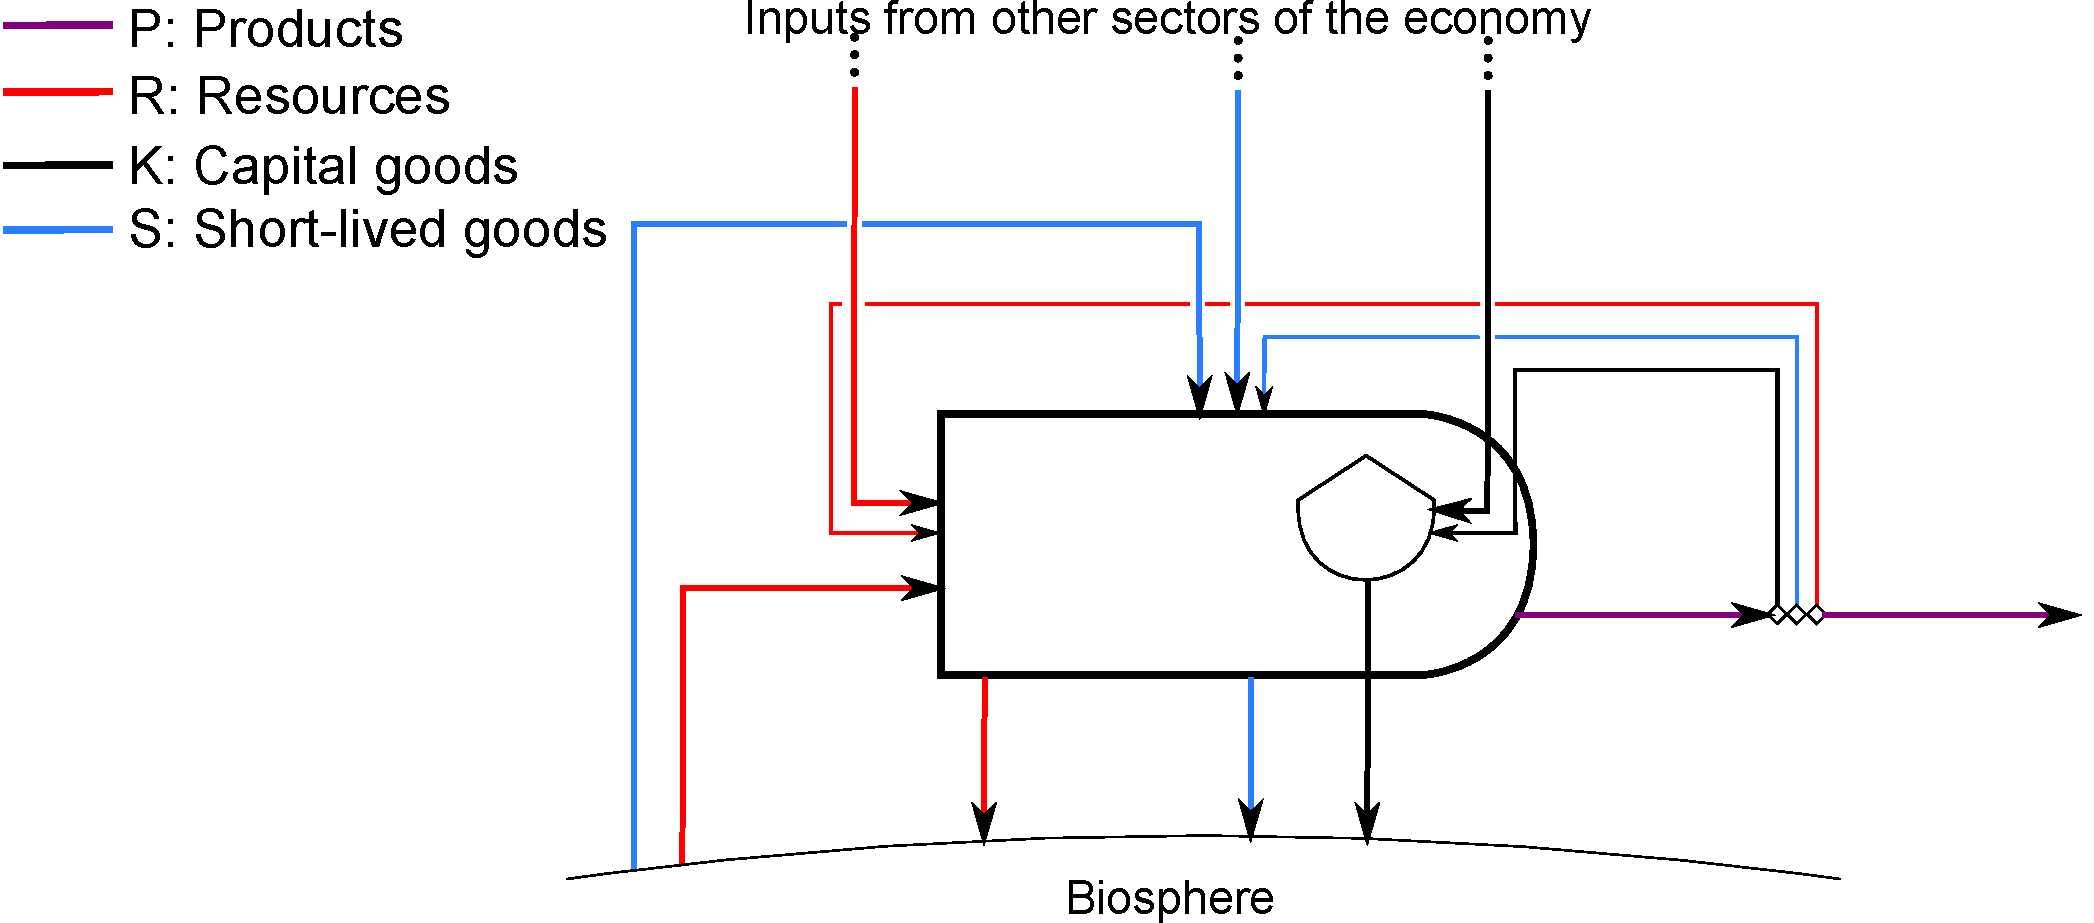
\includegraphics[width=0.8\linewidth]{Part_1/Chapter_Materials/images/PERKS_basic_unit_materials.pdf}
\caption[Material flows into and out of a single sector of the economy.]{Material flows into and out of a single sector of the economy. Resource flows ($\dot{R}$) enter the sector from the left and are embodied in products ($\dot{P}$) which leave from the right. Some waste resources are leave the sector at the bottom and are returned to the biosphere. Short-lived material flows ($\dot{S}$) enter the sector from above and leave from below to return to the biosphere.  Only capital flows ($\dot{K}$) may accumulate within the sector, depicted by the storage tank. These also enter the sector from above. Depreciated capital leaves the sector from below and is returned to the biosphere.}
\label{fig:PERKS_materials}
\end{figure}

Resource materials ($\dot{R}$)\nomenclature{$\dot{R}$}{resource flow rate} 
enter the sector on the left 
and comprise those materials that are destined to be \emph{embodied} 
in the goods produced by the sector ($\dot{P}$)\nomenclature{$\dot{P}$}{product flow rate} , 
except for some proportion that are wasted.
Wastes depart from the bottom of the sector and are
returned to the biosphere. 
For example, sheet metal, rubber, and glass
(as well as many other materials) 
enter the automobile sector as resources 
and end up as material parts of the cars that are produced. 
Some fraction of these resources ($\dot{R}$) may not make it into the final product, 
such as trimming scrap from metal parts stamping, 
and may be either recycled internally, 
or wasted to the biosphere. 
Resource materials are not accumulated within a sector.

Short-lived goods ($\dot{S}$)\nomenclature{$\dot{S}$}{short-lived goods flow rate}  
include those materials 
that are necessary for the production processes of a sector, 
but are neither accumulated within the sector, 
nor destined to be materially part of the product of the sector. 
They enter the sector from above and leave the sector from
below and return to the biosphere. 
Examples of these short-lived flows include energy resources, such as
the electricity needed to run automobile factories,
including any contribution from labor, 
and water used by the sector. 

A number of material flows, such as production equipment,
are necessary for the continued operation of a sector 
but are not counted as short-lived goods, 
because the operation of the sector is dependent 
upon the accumulation of these materials within the sector. 
Such flows are counted as capital goods ($\dot{K}$)
\nomenclature{$\dot{K}$}{capital goods flow rate} . Capital flows also enter from above, 
but are stored within the sector (represented by storage tanks) 
and are returned to the biosphere as capital depreciation from below.
Examples of these capital flows would be the factory and office buildings or
manufacturing equipment within the automobile industry.

All products ($\dot{P}$) leave the right of the sector. 
Some of this $\dot{P}$ flow is returned to the sector as self-consumption 
counted as resources ($\dot{R}$), 
short-lived ($\dot{S}$), or 
capital goods ($\dot{K}$); 
the remainder flows to other sectors within the economy or final demand. 
Within this view, focussing solely on material flows, energy may be accounted
as either an $\dot{R}$ flow, when the energy inflow is \emph{literally} embodied
within the outflowing product $\dot{P}$, such as crude oil converted into
gasoline within a refinery, or as an $\dot{S}$ flow, when the inflowing energy
is not literally embodied within the product. Examples include the electricity
use by an automobile factor, but also the coal or natural gas flowing into a
power plant, since the incoming chemical elements (carbon and hydrogen) \emph{do
not} travel through the electricity transmission lines.

% ****BRH says, we should say something
% about Energy here.****




%%%%%%%%%% Materials: Example A %%%%%%%%%%
\section{Example A: one sector economy}
\label{sec:A_materials}
%%%%%%%%%%

Our first example looks at the case where all processes within the economy occur within
one sector---society (1)---which exchanges materials with the biosphere (0) as depicted in
Figure \ref{fig:A_materials}.  We do not distinguish between production and consumption.



\begin{figure}[h!]
\centering
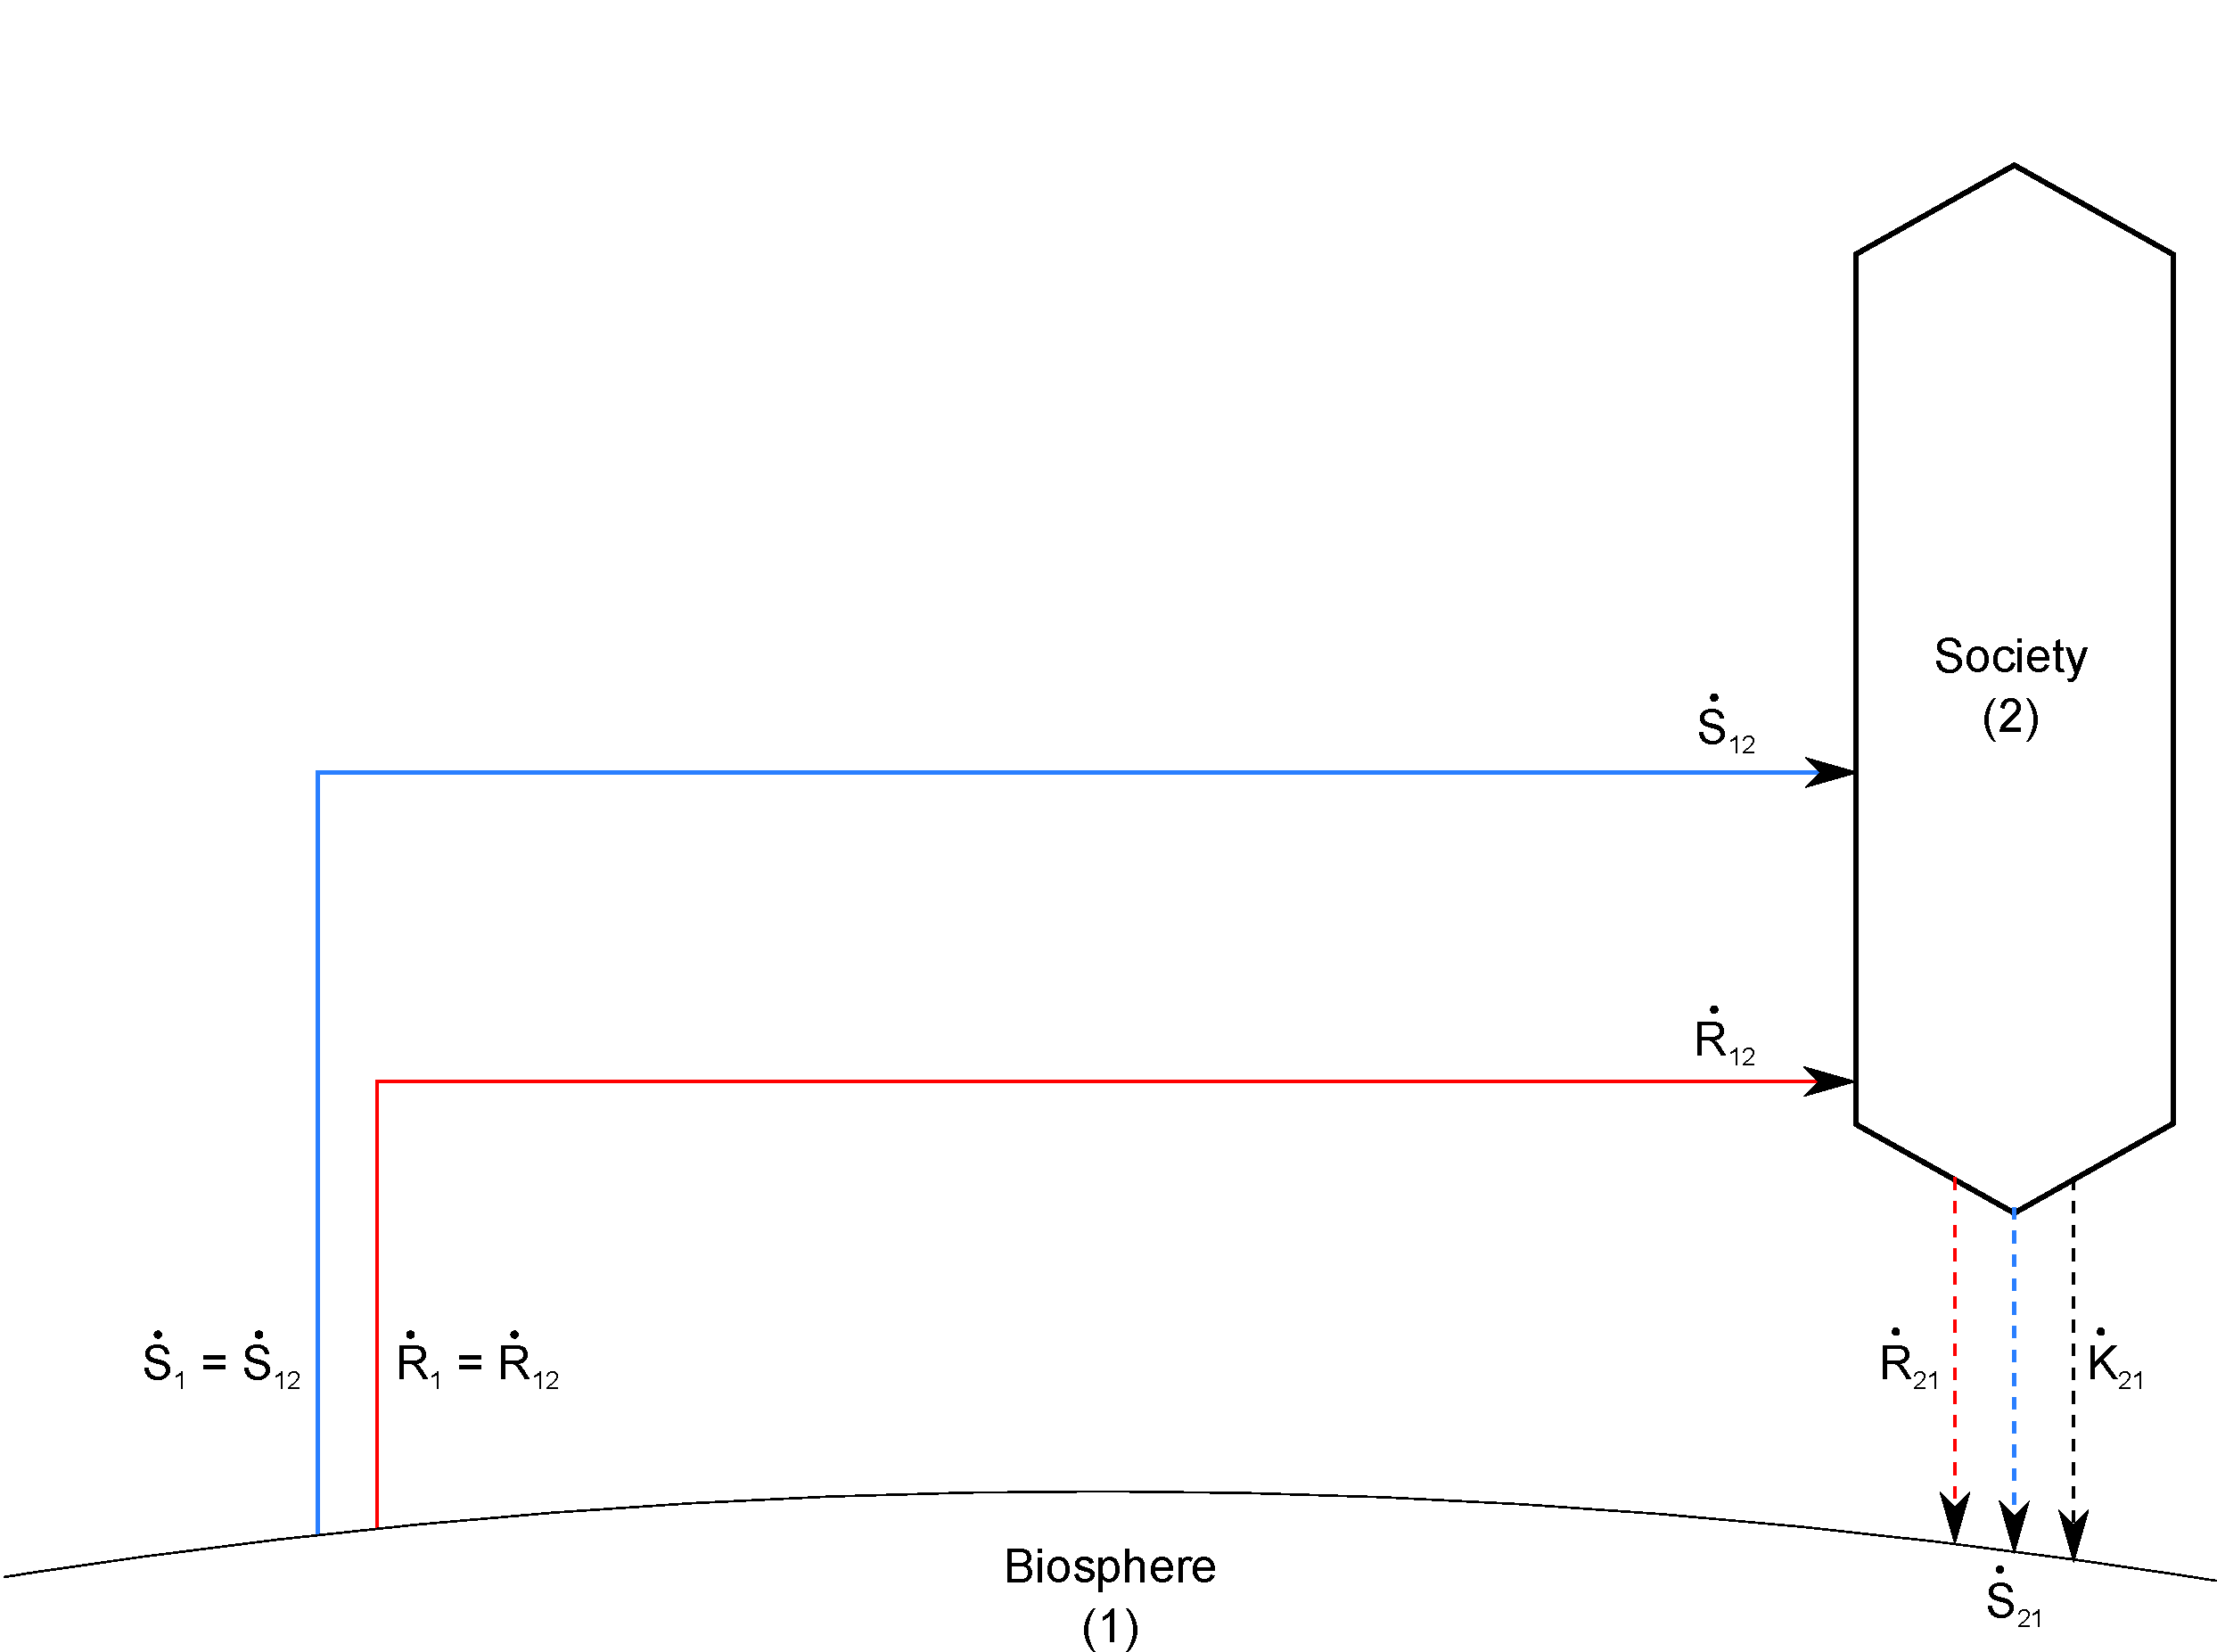
\includegraphics[width=0.8\linewidth]{Part_1/Chapter_Materials/images/1_sector_materials.pdf}
\caption{Flows of materials for a one-sector economy}{Flows of materials for a one-sector economy. 
Resources ($\dot{R}_{01}$) and short-lived materials ($\dot{S}_{01}$) flow into the economy (1) 
from the biosphere (0). Waste resources ($\dot{R}_{10}$) short-lived materials/goods 
($\dot{S}_{10}$) and capital goods ($\dot{K}_{10}$) are returned to the biosphere.}
\label{fig:A_materials}
\end{figure}

Resources, or perhaps more accurately raw materials, ($\dot{R}_{01}$), such as crude oil or iron ore, 
and short-lived materials ($\dot{S}_{01}$), such as oxygen or water that flow \emph{through} economic
processes but are not embodied in the product output, flow into the economy (1) from the biosphere (0). 
These materials are processed within the economy into resource goods, short-lived goods and
capital goods ($\dot{K}$) which are able to be accumulated at some rate $\frac{\mathrm{d}K_{1}}{\mathrm{d}t}$.
Waste resources ($\dot{R}_{10}$) and used short-lived materials/goods ($\dot{S}_{10}$)
are returned to the biosphere without accumulating. Capital goods ($\dot{K}_{10}$) are returned
to the biosphere upon depreciation.

Drawing control volumes around both the biosphere (0) and the economy (1), we can consruct
our material accounting equations, such that:

\begin{align}
\label{eq:A_CV_0_to_1}
	\frac{\mathrm{d}R_0}{\mathrm{d}t}		
	+	\frac{\mathrm{d}S_0}{\mathrm{d}t}
	+	\frac{\mathrm{d}K_0}{\mathrm{d}t}		&	
	=	\dot{R}_{10}		
	+	\dot{S}_{10}	
	+	\dot{K}_{10}											
	-	\dot{R}_{0}											
	-	\dot{S}_{0}								\\
\label{eq:A_CV_0_to_1a}
	\frac{\mathrm{d}R_{1}}{\mathrm{d}t}
	+ \frac{\mathrm{d}S_{1}}{\mathrm{d}t}
	+ \frac{\mathrm{d}K_{1}}{\mathrm{d}t}		&
	= \dot{R}_{01} 
	+ \dot{S}_{01} + \dot{S}_{11}
	- \dot{S}_{1}				
	- \dot{R}_{10}				
	- \dot{S}_{10}				
	- \dot{K}_{10}											
\end{align}

\noindent Remembering that neither resources nor short-lived goods accumulate within economic sectors, tells us that:

\begin{equation}\label{eq:A-dS_1/dt_zero}
	\frac{\mathrm{d}S_1}{\mathrm{d}t}
	= \frac{\mathrm{d}R_1}{\mathrm{d}t}
	= 0.
\end{equation}

\noindent Additionally, we may also say that:

\begin{equation}\label{eq:A_S11}
	\dot{S}_{11} = \dot{S}_{1},
\end{equation}

\noindent such that our material balance equations \ref{eq:A_CV_0_to_1} and \ref{eq:A_CV_0_to_1a} 
become:

%****BRH says, shouldn't this word be
%"accounting" -- not accumulation -- given that is what we
%called it in the sentence introducing eq. 2.4. Or, should we change "accounting" above to accumulation?
%Or, are they synonyms? And, aren't there two of these equations? 2.4 and 2.5? I added a separate
%label for eqn. 2.5**** MIK - Agreed, changed to 'material balance'

\begin{align}\label{eq:A_CV_0_to_1_b}
	\frac{\mathrm{d}R_0}{\mathrm{d}t}		
	+	\frac{\mathrm{d}S_0}{\mathrm{d}t}
	+	\frac{\mathrm{d}K_0}{\mathrm{d}t}		&	
	=	\dot{R}_{10}		
	+	\dot{S}_{10}	
	+	\dot{K}_{10}											
	-	\dot{R}_{0}											
	-	\dot{S}_{0}								\\
	\frac{\mathrm{d}K_{1}}{\mathrm{d}t}		&
	= \dot{R}_{01} 
	+ \dot{S}_{01} 
	- \dot{R}_{10}				
	- \dot{S}_{10}				
	- \dot{K}_{10}											
\end{align}

\noindent Because the only "capital" that accumulates in the biosphere is that which is a waste flow (capital depreciation)
from the economy, e.g. worn-out machines in the scrap yard, we may say that:

\begin{equation} \label{eq:A_K0_balance}
	\frac{\mathrm{d}K_{0}}{\mathrm{d}t}		
	= \dot{K}_{10}
\end{equation}


%%%%%%%%%% Materials: Example B %%%%%%%%%%
\newpage
\section{Example B: two sector economy}
\label{sec:B_materials}
%%%%%%%%%%

In our second example B, we split society into two sectors: production and consumption as depicted in Figure \ref{fig:B_materials}. 

\begin{figure}[h!]
\centering
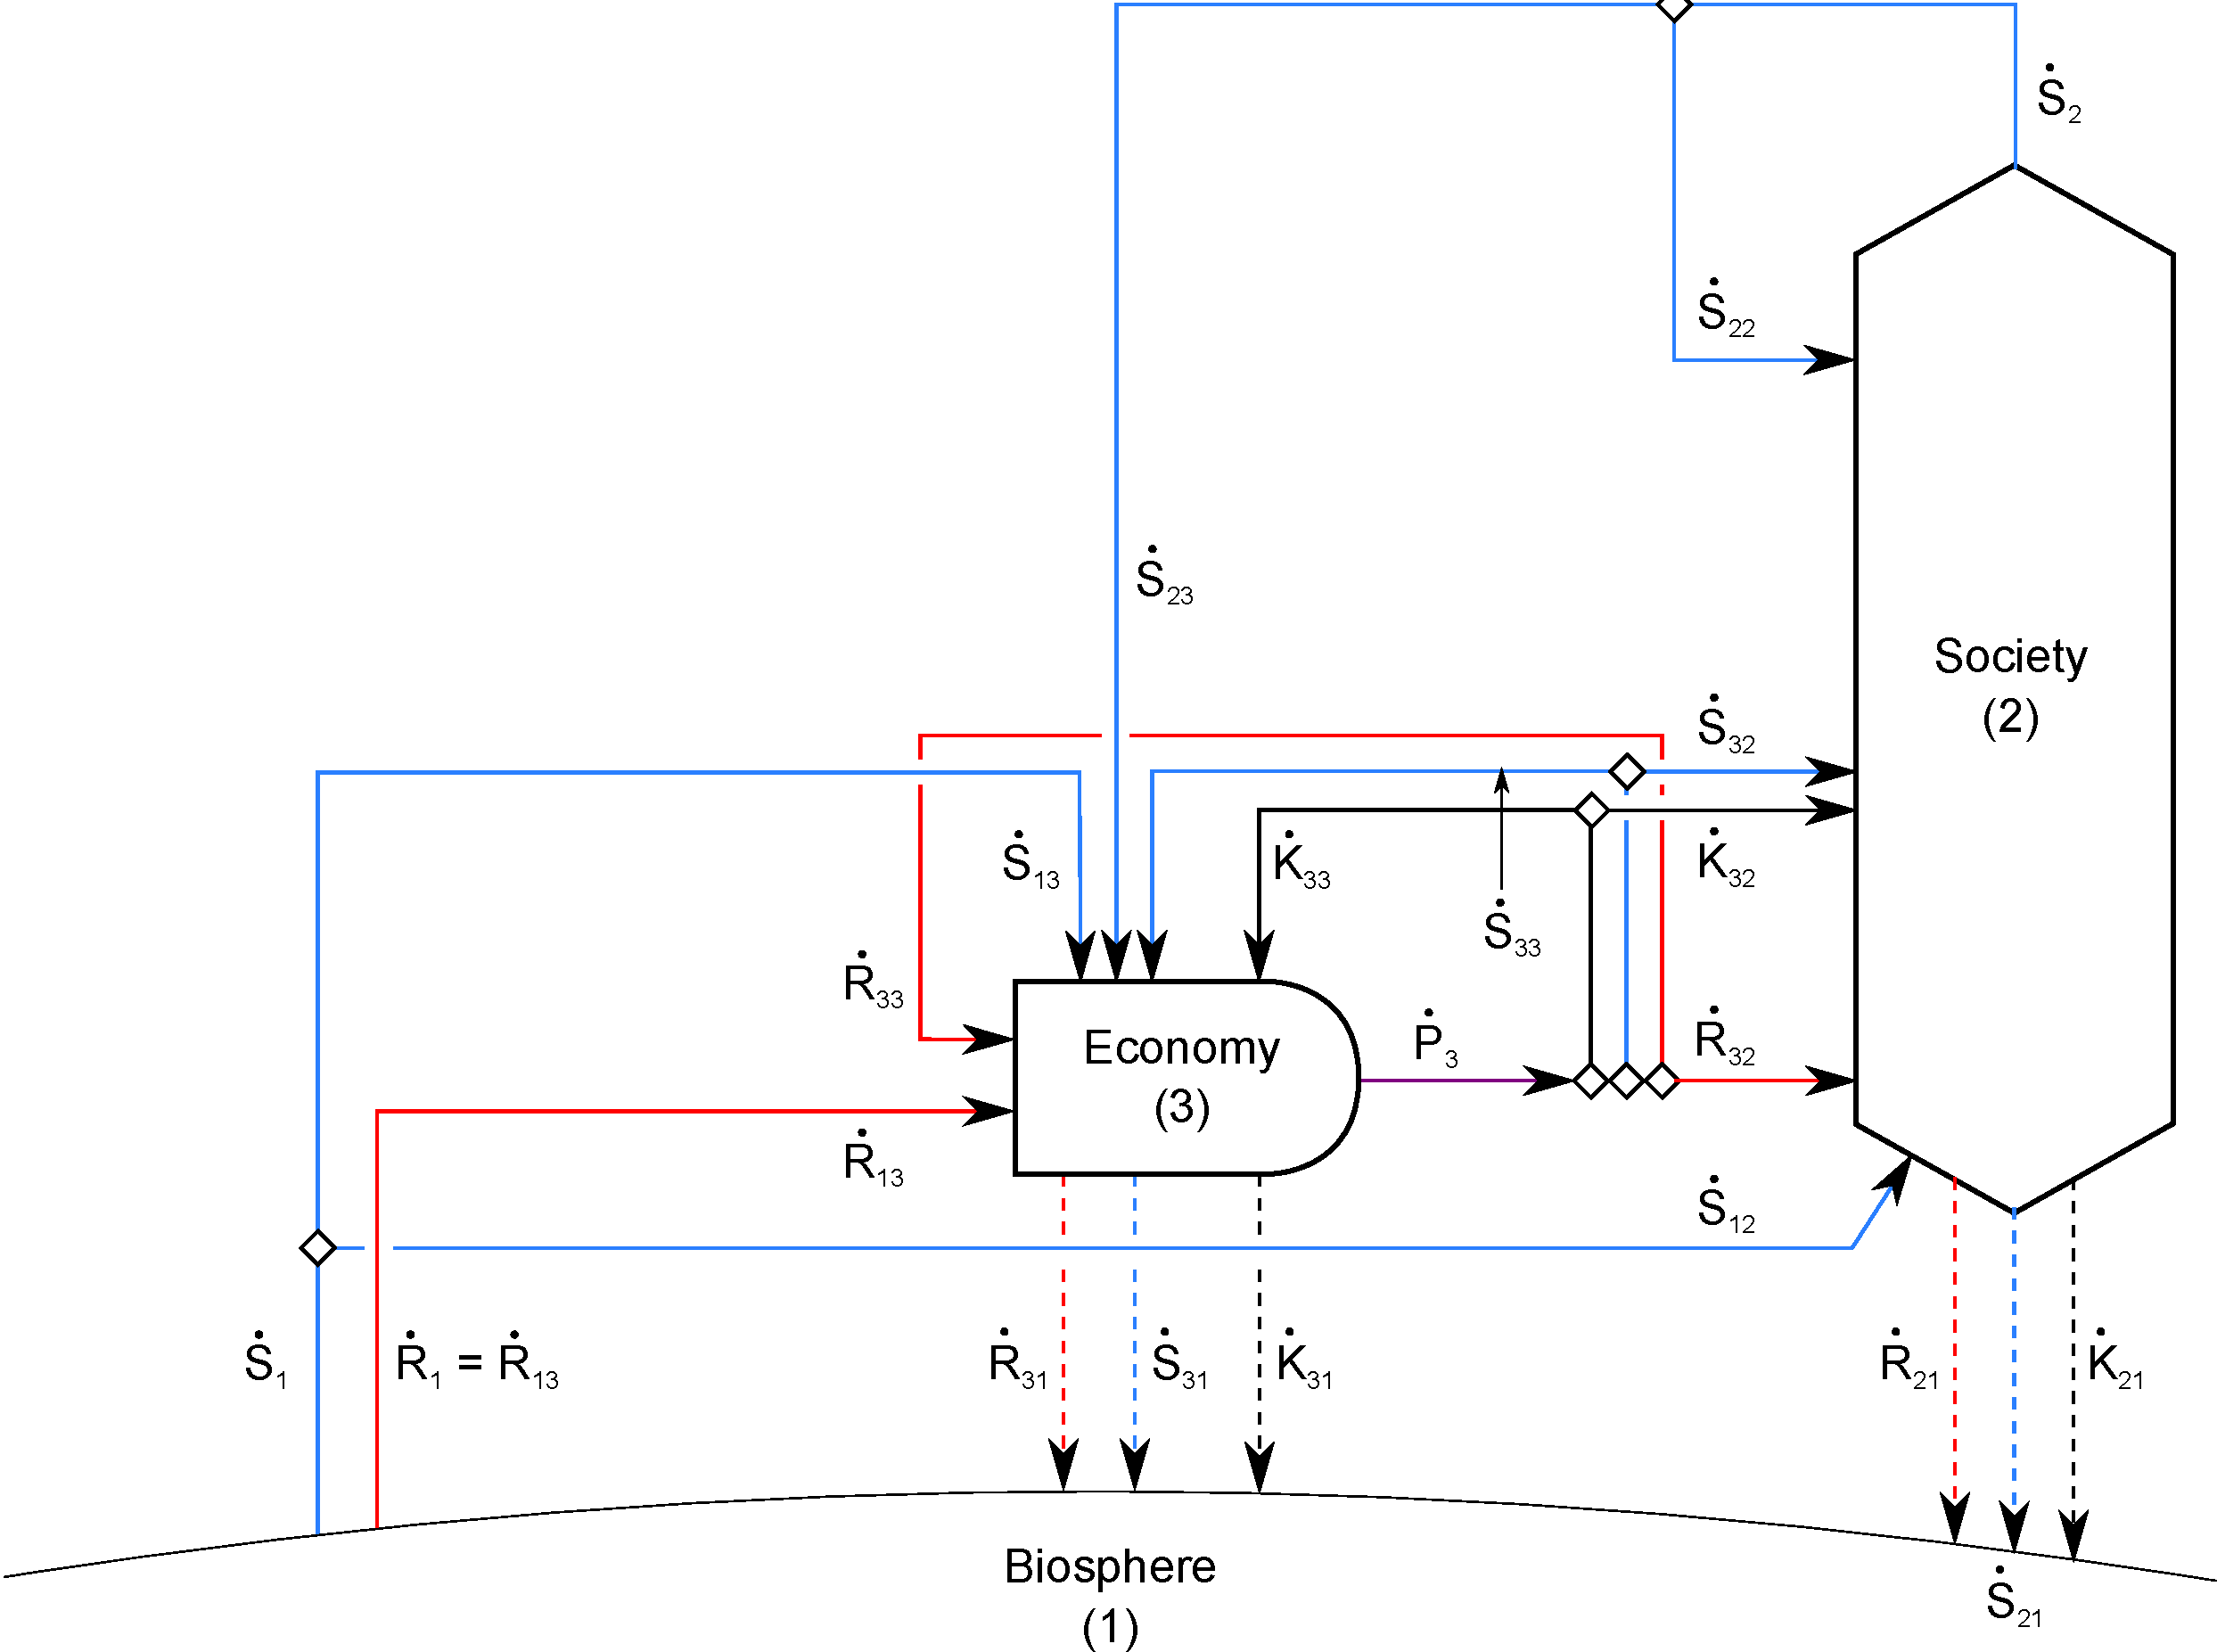
\includegraphics[width=0.8\linewidth]{Part_1/Chapter_Materials/images/2_sector_materials.pdf}
\caption{Flows of materials for a two-sector economy}{Flows of materials for a two-sector economy}
\label{fig:B_materials}
\end{figure}

Sector 2 produces goods and services for consumption in society (1). Again, setting control volumes around the biosphere and our two sectors, our accumulation equations are now written:

\begin{align} \label{eq:B_CV_0_to_2}
	\frac{\mathrm{d}R_{0}}{\mathrm{d}t} 
	+ \frac{\mathrm{d}S_{0}}{\mathrm{d}t}	
	+ \frac{\mathrm{d}K_0}{\mathrm{d}t}		&
	=  \dot{R}_{10} + \dot{R}_{20} 
	+ \dot{S}_{10} + \dot{S}_{20} 
	+ \dot{K}_{10} + \dot{K}_{20} 
	- \dot{R}_{0} 
	- \dot{S}_{0} 							\\
	\frac{\mathrm{d}R_{1}}{\mathrm{d}t} 
	+ \frac{\mathrm{d}S_{1}}{\mathrm{d}t}	
	+ \frac{\mathrm{d}K_{1}}{\mathrm{d}t}	&
	=  \dot{R}_{21} 
	+ \dot{S}_{01} 
	+ \dot{S}_{11} 
	+ \dot{S}_{21}
	+ \dot{K}_{21}
	- \dot{S}_{1} 
	- \dot{R}_{10} 
	- \dot{S}_{10} 
	- \dot{K}_{10},							\\
	\frac{\mathrm{d}R_{2}}{\mathrm{d}t} 
	+ \frac{\mathrm{d}S_{2}}{\mathrm{d}t}
	+ \frac{\mathrm{d}K_{2}}{\mathrm{d}t}	&
	=  \dot{R}_{02} 
	+ \dot{R}_{22} 
	+ \dot{S}_{02} 
	+ \dot{S}_{12} 
	+ \dot{S}_{22} 
	+ \dot{K}_{22}
	- \dot{P}_{2}
	- \dot{R}_{20} 
	- \dot{S}_{20} 
	- \dot{K}_{20},
\end{align}

\begin{equation}
	\dot{R}_{0} = \dot{R}_{02}
\end{equation}

\begin{align}\label{eq:B_S_def}
	\dot{S}_{0} = 
	& \dot{S}_{01} + \dot{S}_{02};
	& \dot{S}_{1} = 
	\dot{S}_{11} + \dot{S}_{12}
\end{align}

Since only capital flows ($\dot{K}$) may be accumulated and are dependent only on flows of capital in and depreciation of capital, we may define capital balance equations:

\begin{equation} \label{eq:B_K1_balance}
	\frac{\mathrm{d}K_{1}}{\mathrm{d}t}
	=  \dot{K}_{12} - \dot{K}_{20},
\end{equation}

[NOT SURE IF THIS IS TRUE IF WE THINK OF $\dot{R}_{12}$ AS FOOD AND $K_{1}$ AS INCLUDING HUMANS... YES, I THINK $\dot{R}_{12}$ CAN BE TURNED INTO  $\dot{K}_{1}$ INTERNALLY, AS THE ACCUMULATION OF (LITERAL) HUMAN CAPITAL, I.E. POPULATION]

\begin{equation} \label{eq:B_K2_balance}
	\frac{\mathrm{d}K_{2}}{\mathrm{d}t}
	=  \dot{K}_{22} - \dot{K}_{20},
\end{equation}

\begin{equation} \label{eq:B_P_def}
	\dot{P}_{2}
	= \dot{R}_{21}
	+ \dot{R}_{22}
	+ \dot{S}_{21}
	+ \dot{S}_{22}
	+ \dot{K}_{21}	 
	+ \dot{K}_{22},
\end{equation}


\noindent Again, remembering that resources and short-lived
goods do not accumulate within sectors of the economy:

\begin{equation}\label{eq:dR_and_dS_zero}
	\frac{\mathrm{d}R_{1}}{\mathrm{d}t}
	= \frac{\mathrm{d}R_{2}}{\mathrm{d}t} 
	= \frac{\mathrm{d}S_{1}}{\mathrm{d}t} 
	= \frac{\mathrm{d}S_{2}}{\mathrm{d}t} 
	= 0,
\end{equation}

\noindent and substituting equations \ref{eq:B_S_def},
\ref{eq:B_K2_balance}  and \ref{eq:B_P_def}, our balance 
equations may now be written:


\begin{align} \label{eq:B_CV_0_to_2_b}
	\frac{\mathrm{d}R_{0}}{\mathrm{d}t} 
	+ \frac{\mathrm{d}S_{0}}{\mathrm{d}t}	
	+ \frac{\mathrm{d}K_0}{\mathrm{d}t}		
	& = \dot{R}_{10} + \dot{R}_{20} 
	+ \dot{S}_{10} + \dot{S}_{20} 
	+ \dot{K}_{10} + \dot{K}_{20} 
	- \dot{R}_{0} 
	- \dot{S}_{0} 							\\
	\frac{\mathrm{d}K_{1}}{\mathrm{d}t}	
	& = \dot{R}_{21} 
	+ \dot{S}_{01} 
	+ \dot{S}_{21}
	+ \dot{K}_{21}
	- \dot{S}_{12} 
	- \dot{R}_{10} 
	- \dot{S}_{10} 
	- \dot{K}_{10},							\\
	\dot{K}_{22} - \dot{K}_{20}	
	& = \dot{R}_{02} 
	+ \dot{S}_{02} 
	+ \dot{S}_{12} 
	- \dot{R}_{21}
	- \dot{S}_{21}
	- \dot{K}_{21}
	- \dot{R}_{20} 
	- \dot{S}_{20} 
	- \dot{K}_{20}							\\
\end{align}





%%%%%%%%%% Materials: Example C %%%%%%%%%%
\newpage
\section{Example C: three sector economy}
\label{sec:C_materials}
%%%%%%%%%%

In example C, we differentiate between two production sectors, one produces energy products and one produces other goods and services.

\begin{figure}[h!]
\centering
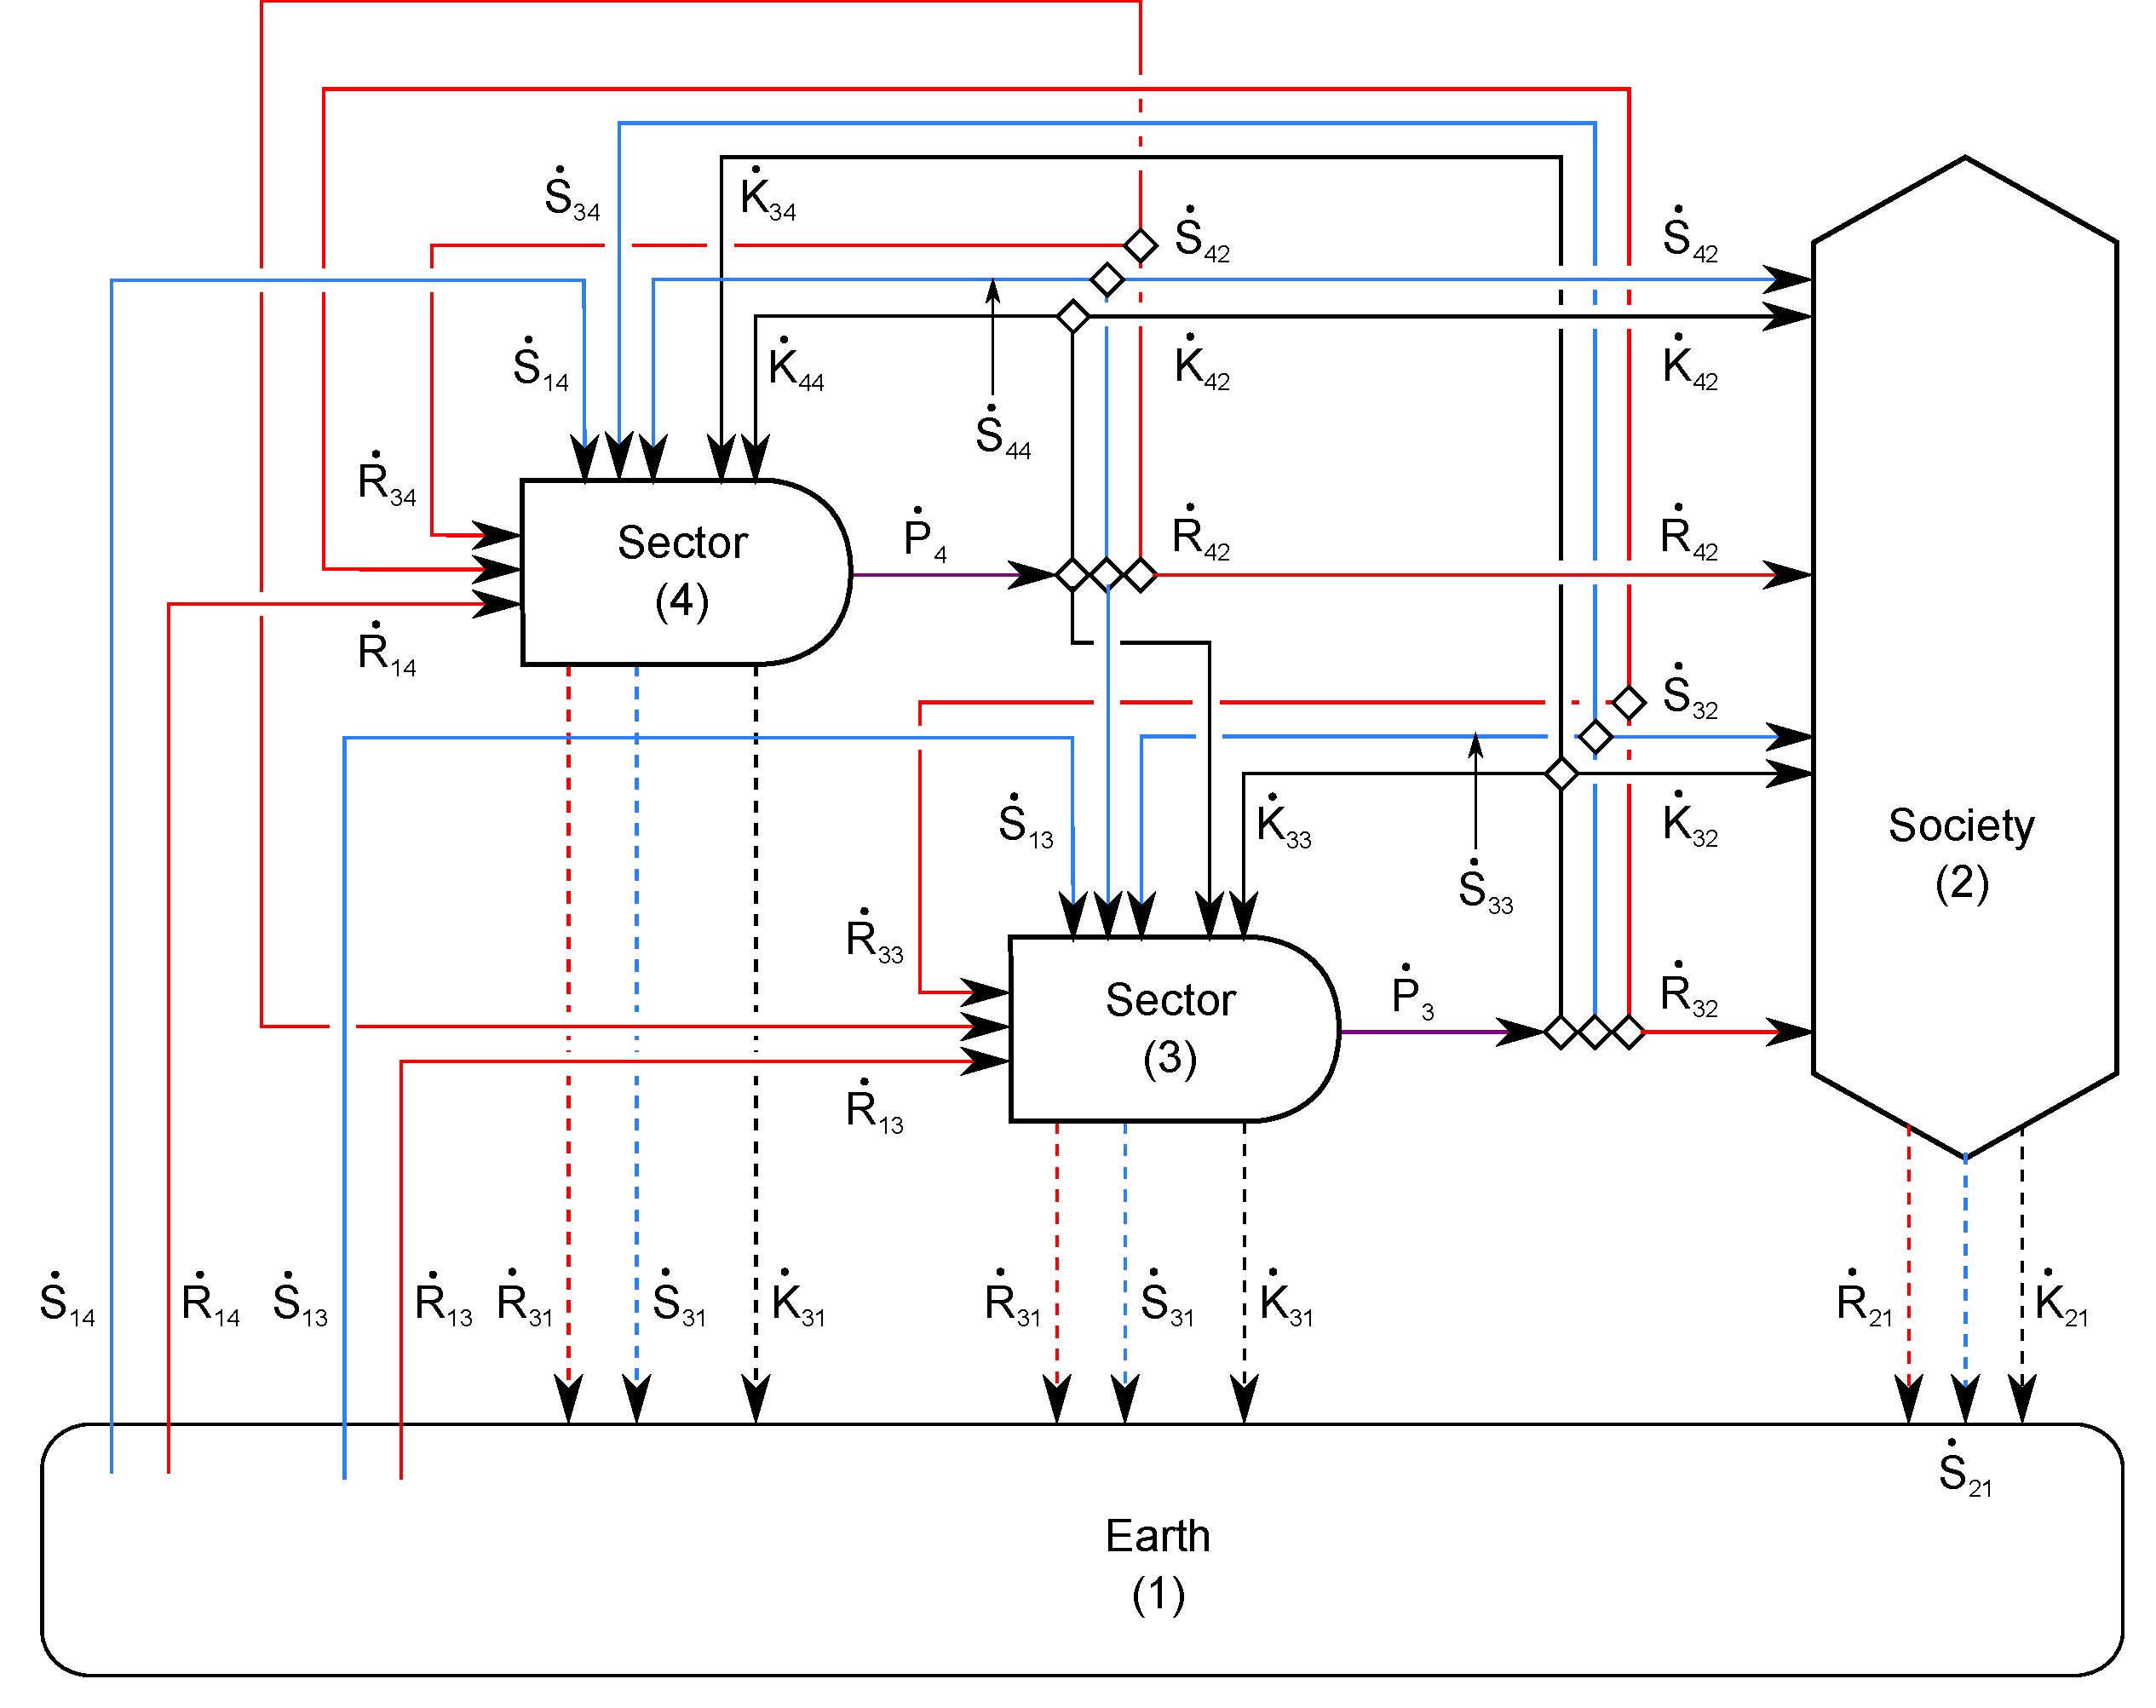
\includegraphics[width=0.8\linewidth]{Part_1/Chapter_Materials/images/3_sector_materials.pdf}
\caption{Flows of materials for a three-sector economy}{Flows of materials for a three-sector economy}
\label{fig:C_materials}
\end{figure}

Accounting for the material flows into and out of the biosphere (sector 0) gives the following equation:

\begin{align} \label{eq:C_CV_0}
	\frac{\mathrm{d}R_{0}}{\mathrm{d}t} 
	+ \frac{\mathrm{d}S_{0}}{\mathrm{d}t}	
	+ \frac{\mathrm{d}K_0}{\mathrm{d}t}		
	& =  \dot{R}_{10} + \dot{R}_{20} + \dot{R}_{30}
	+ \dot{S}_{10} + \dot{S}_{20} + \dot{S}_{30}
	+ \dot{K}_{10} + \dot{K}_{20} + \dot{K}_{30}
	- \dot{R}_{0} 
	- \dot{S}_{0},
\end{align}

\noindent which may be rewritten as:

\begin{align} \label{eq:C_CV_0_b}
	\frac{\mathrm{d}R_{0}}{\mathrm{d}t} 
	+ \frac{\mathrm{d}S_{0}}{\mathrm{d}t}	
	+ \frac{\mathrm{d}K_0}{\mathrm{d}t}		
	& =  \sum_{i = 1}^{3}\dot{R}_{i0}
	+ \sum_{i = 1}^{3}\dot{S}_{i0}
	+ \sum_{i = 1}^{3}\dot{K}_{i0}
	- \dot{R}_{0} 
	- \dot{S}_{0},
\end{align}

Similarly, flows for the other sectors may be written:

\begin{align} \label{eq:C_CV_1_to_3}
	\frac{\mathrm{d}K_{1}}{\mathrm{d}t}		
	& =  \dot{R}_{01} 
	+ \dot{S}_{01}
	+ \sum_{i = 1}^{3}\dot{R}_{i1}
	+ \sum_{i = 1}^{3}\dot{S}_{i1}
	+ \sum_{i = 1}^{3}\dot{K}_{i1}
	- \dot{P}_{1}
	- \dot{R}_{10} 
	- \dot{S}_{10}
	- \dot{K}_{10},										\\
	\frac{\mathrm{d}K_{2}}{\mathrm{d}t}		
	& =  \dot{R}_{02} 
	+ \dot{S}_{02}
	+ \sum_{i = 1}^{3}\dot{R}_{i2}
	+ \sum_{i = 1}^{3}\dot{S}_{i2}
	+ \sum_{i = 1}^{3}\dot{K}_{i2}
	- \dot{P}_{2}
	- \dot{R}_{20} 
	- \dot{S}_{20}
	- \dot{K}_{20},										\\	
	\frac{\mathrm{d}K_{3}}{\mathrm{d}t}		
	& =  \dot{R}_{03} 
	+ \dot{S}_{03}
	+ \sum_{i = 1}^{3}\dot{R}_{i3}
	+ \sum_{i = 1}^{3}\dot{S}_{i3}
	+ \sum_{i = 1}^{3}\dot{K}_{i3}
	- \dot{P}_{3}
	- \dot{R}_{30} 
	- \dot{S}_{30}
	- \dot{K}_{30}.										
\end{align}

These equations may be summarized in one single equation as:

\begin{align} \label{eq:C_CV_1_to_3_b}
	\frac{\mathrm{d}K_{j}}{\mathrm{d}t}		
	& =  \dot{R}_{0j} 
	+ \dot{S}_{0j}
	+ \sum_{i = 1}^{3}\dot{R}_{ij}
	+ \sum_{i = 1}^{3}\dot{S}_{ij}
	+ \sum_{i = 1}^{3}\dot{K}_{ij}
	- \dot{P}_{j}
	- \dot{R}_{j0} 
	- \dot{S}_{j0}
	- \dot{K}_{j0};
	& j \in \left[1,3\right].
\end{align}

Again, we can say that:

\begin{align} \label{eq:C_CV_K_balance}
	\frac{\mathrm{d}K_{j}}{\mathrm{d}t}		
	& =  \sum_{i = 1}^{3}\dot{K}_{ij}
	- \dot{K}_{j0};
\end{align}

\noindent hence we may say that:

\begin{align} \label{eq:C_CV_1_to_3_b}
	\dot{R}_{0j} 
	+ \dot{S}_{0j}
	+ \sum_{i = 1}^{3}\dot{R}_{ij}
	+ \sum_{i = 1}^{3}\dot{S}_{ij}
	& = \dot{P}_{j}
	- \dot{R}_{j0} 
	- \dot{S}_{j0}.
\end{align}



\begin{figure}[h!]
\centering
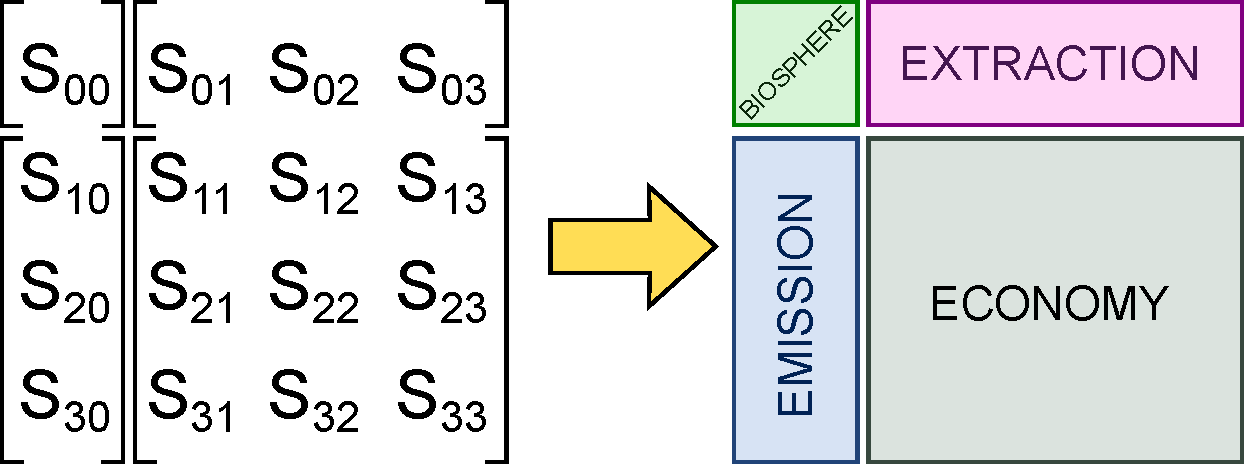
\includegraphics[width=0.8\linewidth]{Part_1/Chapter_Materials/images/Matrix.pdf}
\caption{The matrix of biosphere-economy flows}{The matrix of biosphere-economy flows}
\label{fig:C_mat_matrix}
\end{figure}

%%%%%%%%%% Materials: Auto industry example %%%%%%%%%%
\section{Materials in the auto industry}
\label{sec:materials_auto}
%%%%%%%%%%

%%%%%%%%%% Materials: Summary %%%%%%%%%%
\section{Summary}
\label{sec:materials_summary}
%%%%%%%%%%

\bibliography{../../EROI_review_v2}
\bibliographystyle{unsrt}


% Always give a unique label
% and use \ref{<label>} for cross-references
% and \cite{<label>} for bibliographic references
% use \sectionmark{}
% to alter or adjust the section heading in the running head
%% Instead of simply listing headings of different levels we recommend to let every heading be followed by at least a short passage of text. Furtheron please use the \LaTeX\ automatism for all your cross-references and citations.

%% Please note that the first line of text that follows a heading is not indented, whereas the first lines of all sequent paragraphs are.

%% Use the standard \verb|equation| environment to typeset your equations, e.g.
%
%% \begin{equation}
%% a \times b = c\;,
%% \end{equation}
%
%% however, for multiline equations we recommend to use the \verb|eqnarray|
%% environment\footnote{In physics texts please activate the class option \texttt{vecphys} to depict your vectors in \textbf{\itshape boldface-italic} type - as is customary for a wide range of physical jects.}.
%%\begin{eqnarray}
%%a \times b = c \nonumber\\
%% \vec{a} \cdot \vec{b}=\vec{c}
%% \label{eq:01}
%%\end{eqnarray}

%% \section{section Heading}
%% \label{sec:2}
%% Instead of simply listing headings of different levels we recommend to let every heading be followed by at least a short passage of text. Furtheron please use the \LaTeX\ automatism for all your cross-references\index{cross-references} and citations\index{citations} as has already been described in Sect.~\ref{sec:2}.

%% \begin{quotation}
%% Please do not use quotation marks when quoting texts! Simply use the \verb|quotation| environment -- it will automatically render Springer's preferred layout.
%% \end{quotation}


%% \section{section Heading}
%% Instead of simply listing headings of different levels we recommend to let every heading be followed by at least a short passage of text. Furtheron please use the \LaTeX\ automatism for all your cross-references and citations as has already been described in Sect.~\ref{sec:2}, see also Fig.~\ref{fig:1}\footnote{If you copy text passages, figures, or tables from other works, you must obtain \textit{permission} from the copyright holder (usually the original publisher). Please enclose the signed permission with the manucript. The sources\index{permission to print} must be acknowledged either in the captions, as footnotes or in a separate section of the book.}

%% Please note that the first line of text that follows a heading is not indented, whereas the first lines of all sequent paragraphs are.

% For figures use
%
%% \begin{figure}[b]
%% \sidecaption
% Use the relevant command for your figure-insertion program
% to insert the figure file.
% For example, with the option graphics use
%% \includegraphics[scale=.65]{figure}
%
% If not, use
%\picplace{5cm}{2cm} % Give the correct figure height and width in cm
%
%% \caption{If the width of the figure is less than 7.8 cm use the \texttt{sidecapion} command to flush the caption on the left side of the page. If the figure is positioned at the top of the page, align the sidecaption with the top of the figure -- to achieve this you simply need to use the optional argument \texttt{[t]} with the \texttt{sidecaption} command}
%% \label{fig:1}       % Give a unique label
%% \end{figure}


%% \paragraph{Paragraph Heading} %
%% Instead of simply listing headings of different levels we recommend to let every heading be followed by at least a short passage of text. Furtheron please use the \LaTeX\ automatism for all your cross-references and citations as has already been described in Sect.~\ref{sec:2}.

%% Please note that the first line of text that follows a heading is not indented, whereas the first lines of all sequent paragraphs are.

%% For typesetting numbered lists we recommend to use the \verb|enumerate| environment -- it will automatically render Springer's preferred layout.

%% \begin{enumerate}
%% \item{Livelihood and survival mobility are oftentimes coutcomes of uneven socioeconomic development.}
%% \begin{enumerate}
%% \item{Livelihood and survival mobility are oftentimes coutcomes of uneven socioeconomic development.}
%% \item{Livelihood and survival mobility are oftentimes coutcomes of uneven socioeconomic development.}
%% \end{enumerate}
%% \item{Livelihood and survival mobility are oftentimes coutcomes of uneven socioeconomic development.}
%% \end{enumerate}


%% \paragraph{paragraph Heading} In order to avoid simply listing headings of different levels we recommend to let every heading be followed by at least a short passage of text. Use the \LaTeX\ automatism for all your cross-references and citations as has already been described in Sect.~\ref{sec:2}, see also Fig.~\ref{fig:2}.

%% Please note that the first line of text that follows a heading is not indented, whereas the first lines of all sequent paragraphs are.

%% For unnumbered list we recommend to use the \verb|itemize| environment -- it will automatically render Springer's preferred layout.

%% \begin{itemize}
%% \item{Livelihood and survival mobility are oftentimes coutcomes of uneven socioeconomic development, cf. Table~\ref{tab:1}.}
%% \begin{itemize}
%% \item{Livelihood and survival mobility are oftentimes coutcomes of uneven socioeconomic development.}
%% \item{Livelihood and survival mobility are oftentimes coutcomes of uneven socioeconomic development.}
%% \end{itemize}
%% \item{Livelihood and survival mobility are oftentimes coutcomes of uneven socioeconomic development.}
%% \end{itemize}

%% \begin{figure}[t]
%% \sidecaption[t]
% Use the relevant command for your figure-insertion program
% to insert the figure file.
% For example, with the option graphics use
%% \includegraphics[scale=.65]{figure}
%
% If not, use
%\picplace{5cm}{2cm} % Give the correct figure height and width in cm
%
%% \caption{Please write your figure caption here}
%% \label{fig:2}       % Give a unique label
%% \end{figure}

%% \runinhead{Run-in Heading Boldface Version} Use the \LaTeX\ automatism for all your cross-references and citations as has already been described in Sect.~\ref{sec:2}.

%% \runinhead{Run-in Heading Italic Version} Use the \LaTeX\ automatism for all your cross-refer\-ences and citations as has already been described in Sect.~\ref{sec:2}\index{paragraph}.
% Use the \index{} command to code your index words
%
% For tables use
%
%% \begin{table}
%% \caption{Please write your table caption here}
%% \label{tab:1}       % Give a unique label
%
% For LaTeX tables use
%
%% \begin{tabular}{p{2cm}p{2.4cm}p{2cm}p{4.9cm}}
%% \hline\noalign{\smallskip}
%% Classes & class & Length & Action Mechanism  \\
%% \noalign{\smallskip}\svhline\noalign{\smallskip}
%% Translation & mRNA$^a$  & 22 (19--25) & Translation repression, mRNA cleavage\\
%% Translation & mRNA cleavage & 21 & mRNA cleavage\\
%% Translation & mRNA  & 21--22 & mRNA cleavage\\
%%Translation & mRNA  & 24--26 & Histone and DNA Modification\\
%%\noalign{\smallskip}\hline\noalign{\smallskip}
%%\end{tabular}
%%$^a$ Table foot note (with superscript)
%%\end{table}
%
%% \section{Section Heading}
%%\label{sec:3}
% Always give a unique label
% and use \ref{<label>} for cross-references
% and \cite{<label>} for bibliographic references
% use \sectionmark{}
% to alter or adjust the section heading in the running head
%% Instead of simply listing headings of different levels we recommend to let every heading be followed by at least a short passage of text. Furtheron please use the \LaTeX\ automatism for all your cross-references and citations as has already been described in Sect.~\ref{sec:2}.

%% Please note that the first line of text that follows a heading is not indented, whereas the first lines of all sequent paragraphs are.

%%If you want to list definitions or the like we recommend to use the Springer-enhanced \verb|description| environment -- it will automatically render Springer's preferred layout.

%%\begin{description}[Type 1]
%%\item[Type 1]{That addresses central themes pertainng to migration, health, and disease. In Sect.~\ref{sec:1}, Wilson discusses the role of human migration in infectious disease distributions and patterns.}
%%\item[Type 2]{That addresses central themes pertainng to migration, health, and disease. In Sect.~\ref{sec:2}, Wilson discusses the role of human migration in infectious disease distributions and patterns.}
%%\end{description}

%%\section{section Heading} %
%% In order to avoid simply listing headings of different levels we recommend to let every heading be followed by at least a short passage of text. Use the \LaTeX\ automatism for all your cross-references and citations citations as has already been described in Sect.~\ref{sec:2}.

%% Please note that the first line of text that follows a heading is not indented, whereas the first lines of all sequent paragraphs are.

%% \begin{svgraybox}
%% If you want to emphasize complete paragraphs of texts we recommend to use the newly defined Springer class option \verb|graybox| and the newly defined environment \verb|svgraybox|. This will produce a 15 percent screened box 'behind' your text.

%% If you want to emphasize complete paragraphs of texts we recommend to use the newly defined Springer class option and environment \verb|svgraybox|. This will produce a 15 percent screened box 'behind' your text.
%% \end{svgraybox}


%% \section{section Heading}
%%Instead of simply listing headings of different levels we recommend to let every heading be followed by at least a short passage of text. Furtheron please use the \LaTeX\ automatism for all your cross-references and citations as has already been described in Sect.~\ref{sec:2}.

%% Please note that the first line of text that follows a heading is not indented, whereas the first lines of all sequent paragraphs are.

%% \begin{theorem}
%% Theorem text goes here.
%% \end{theorem}
%
% or
%
%% \begin{definition}
%% Definition text goes here.
%% \end{definition}

%% \begin{proof}
%\smartqed
%% Proof text goes here.
%% \qed
%% \end{proof}

%%\paragraph{Paragraph Heading} %
%% Instead of simply listing headings of different levels we recommend to let every heading be followed by at least a short passage of text. Furtheron please use the \LaTeX\ automatism for all your cross-references and citations as has already been described in Sect.~\ref{sec:2}.

%% Note that the first line of text that follows a heading is not indented, whereas the first lines of all subsequent paragraphs are.
%
% For built-in environments use
%
%%\begin{theorem}
%%Theorem text goes here.
%%\end{theorem}
%
%%\begin{definition}
%%Definition text goes here.
%%\end{definition}
%
%%\begin{proof}
%%\smartqed
%% Proof text goes here.
%%\qed
%%\end{proof}
%
%% \begin{acknowledgement}
%% If you want to include acknowledgments of assistance and the like at the end of an individual chapter please use the \verb|acknowledgement| environment -- it will automatically render Springer's preferred layout.
%% \end{acknowledgement}
%
%% \section*{Appendix}
%% \addcontentsline{toc}{section}{Appendix}
%
%% When placed at the end of a chapter or contribution (as opposed to at the end of the book), the numbering of tables, figures, and equations in the appendix section continues on from that in the main text. Hence please \textit{do not} use the \verb|appendix| command when writing an appendix at the end of your chapter or contribution. If there is only one the appendix is designated ``Appendix'', or ``Appendix 1'', or ``Appendix 2'', etc. if there is more than one.

%% \begin{equation}
%% a \times b = c
%% \end{equation}
% Problems or Exercises should be sorted chapterwise
%% \section*{Problems}
%% \addcontentsline{toc}{section}{Problems}
%
% Use the following environment.
% Don't forget to label each problem;
% the label is needed for the solutions' environment
%% \begin{prob}
%% \label{prob1}
%% A given problem or Excercise is described here. The
%% problem is described here. The problem is described here.
%% \end{prob}

%% \begin{prob}
%% \label{prob2}
%% \textbf{Problem Heading}\\
%% (a) The first part of the problem is described here.\\
%% (b) The second part of the problem is described here.
%% \end{prob}




%!TEX root = ../../Heun_Dale_Haney_A_dynamic_approach_to_input_output_modeling.tex
%%%%%%%%%%%%%%%%%%%%% chapter.tex %%%%%%%%%%%%%%%%%%%%%%%%%%%%%%%%%
%
% sample chapter
%
% Use this file as a template for your own input.
%
%%%%%%%%%%%%%%%%%%%%%%%% Springer-Verlag %%%%%%%%%%%%%%%%%%%%%%%%%%
%\motto{Use the template \emph{chapter.tex} to style the various elements of your chapter content.}
\motto{Living organisms need to be open 
to a constant flow of resources~(energy and matter) 
to stay alive; \\
human organizations need to be open 
to a flow of mental resources~(information and ideas), 
as well as to the flows of energy and materials 
that are part of the production \\
of goods or services.~\emph{\cite[p.117]{Capra2004}}

\hfill---\emph{Fritjof Capra}}

%%%%%%%%%%%%%%%%%%%%%%%%%%%%%%%%%%%%%%%%%
%%%%%%%%%% Direct Energy Flows %%%%%%%%%%
%%%%%%%%%%%%%%%%%%%%%%%%%%%%%%%%%%%%%%%%%
\chapter{Flows of direct energy }
% Always give a unique label
\label{chap:direct_energy} 
% use \chaptermark{} to alter or adjust the chapter heading in the running head
\chaptermark{Direct energy}
%%%%%%%%%%%%%%%%%%%%%%%%%%%%%%%%%%%%%%%%%
%%%%%%%%%%%%%%%%%%%%%%%%%%%%%%%%%%%%%%%%%
%%%%%%%%%%%%%%%%%%%%%%%%%%%%%%%%%%%%%%%%%

%% \abstract{Each chapter should be preceded by an abstract (10--15 lines long) that summarizes the content. The abstract will appear \textit{online} at \url{www.SpringerLink.com} and be available with unrestricted access. This allows unregistered users to read the abstract as a teaser for the complete chapter. As a general rule the abstracts will not appear in the printed version of your book unless it is the style of your particular book or that of the series to which your book belongs.\newline\indent
%% Please use the 'starred' version of the new Springer \texttt{abstract} command for typesetting the text of the online abstracts (cf. source file of this chapter template \texttt{abstract}) and include them with the source files of your manuscript. Use the plain \texttt{abstract} command if the abstract is also to appear in the printed version of the book.}

%% Use the template \emph{chapter.tex} together with the Springer document class SVMono (monograph-type books) or SVMult (edited books) to style the various elements of your chapter content in the Springer layout.

\abstract*{In this chapter, we develop equations, 
assisted by the First Law of Thermodynamics,
that describe the flow of 
direct energy through economies.
The equations are applied to
example economies with increasing levels of disaggregation. 
Finally, the energy flows for our running example, the US auto industry,
are discussed.}




In Chapters~\ref{chap:intro} and~\ref{chap:acct_for_won}, 
we showed that energy consumption is intimately linked to economic activity
and established the metabolism metaphor for the economy.
From the metabolism metaphor, we understand that the economy 
consists of producers and consumers who exchange
goods and services and factors of production 
while extracting resources from and disposing wastes to the biosphere. 
In Chapter~\ref{chap:materials}, we established the material basis of economies: 
economies processes
raw resources for the benefit of producers and consumers 
while generating unavoidable wastes.
In this chapter, we describe and analyze the 
direct energy
that is associated with economic activity within an economy.

All forms of energy provide the potential% 
	\footnote{
	The quantification of the mechanical work potential of energy is \emph{exergy}.
	When energy is ``consumed'' by an economy, exergy (work potential) is destroyed.
	These topics are discussed in greater detail in Section~\ref{sec:material_quality}.
	}
to do mechanical work.%
	\footnote{
	Mechanical work is the product of a force and the distance
	through which it acts.
	}
Energy (as mechanical work) 
is an essential aspect of the metabolic economy;
with it, materials are refined, shaped, and assembled
into useful intermediate and final products; 
food is made available to people in society; 
jobs are made easier for workers;
human ingenuity is multiplied;
and complex systems and civilizations are possible.
In the absence of high rates of energy available at low cost,
life becomes much more difficult, even impossible, for many people.

The analogy for this chapter is this: 
energy is to thermodynamics as money is to financial accounting.
Or, energy is the \emph{currency of thermodynamics}.
Just as an accountant understands a firm by watching how and where
currency flows through it, so we can understand an economy by watching
how and where energy flows through it.
Accounting for energy flows through an economy
is essential for developing a dynamic picture 
of its metabolism.

The purpose of this chapter is to develop 
a framework for accounting energy flows within economies.
To do so, we will employ the First Law of Thermodynamics
which tells us that
the quantity of energy is conserved in every process.%
	\footnote{
	The First Law
	does not speak about the quality of energy---not
	all forms of energy are equally \emph{useful}.
	There are several ways to assess the quality of energy.
	Hammond and Winnett note 
	the importance of the concept of \emph{exergy}
	to describe the maximum physical work 
	which can be performed by an energy resource
	as it comes into equilibrium with its environment.\cite{Hammond:2009tu}

	The quality of energy can be assessed in terms of economic value, too.
	Some energy resources, such as liquid fuels, 
	are more economically valuable than others,
	i.e.\ within society, there is a preference for these resources,
	such that, ``accounting for energy quality reveals a relatively strong relationship 
	between energy use and economic output.''~\cite[p.~313]{Cleveland2000}
	We see this preference played out on a daily basis
	when coal is converted to electricity at 
	an average efficiency of around one third.
	Society is willing to pay a premium for electricity
	over coal due to its vastly superior usefulness 
	for a multitude of tasks.
	}
With an energy framework in hand, we will be positioned 
to assess the rate at which
consumed direct energy becomes embodied within the products and 
services that an economy provides
(Chapter~\ref{chap:embodied_energy}).


%%%%%%%%%% Energy: Methodology %%%%%%%%%%
\section{Methodology}
\label{sec:energy_methodology}
%%%%%%%%%%

We begin by noting that direct energy travels 
with material through an economy.
``Direct'' energy refers to forms of energy accounted by the 
First Law of Thermodynamics,
including chemical potential energy, 
nuclear potential energy, 
gravitational potential energy,
thermal energy, 
and kinetic energy.
We use the term ``direct'' energy distinct from ``embodied'' energy, 
which will be discussed in Chapter~\ref{chap:embodied_energy}.
Examples of direct energy flows include 
the chemical potential energy of coal inflows to an energy sector, 
the thermal energy of process steam into a textile plant, and
the thermal energy of CO$_2$ automobile exhaust.
Each of these example flows is an example of a ``transfer in''
or a ``transfer out,'' in the language % chktex 38
of Section~\ref{sec:accounting_in_everyday_life}.
In each case, the material (coal, steam, and CO$_2$) 
carries direct energy with it.
Figure~\ref{fig:PERKS_energy_content} shows a corresponding 
direct energy flow for each material flow of Figure~\ref{fig:PERKS_materials}.

\begin{figure}[!ht]
\centering\
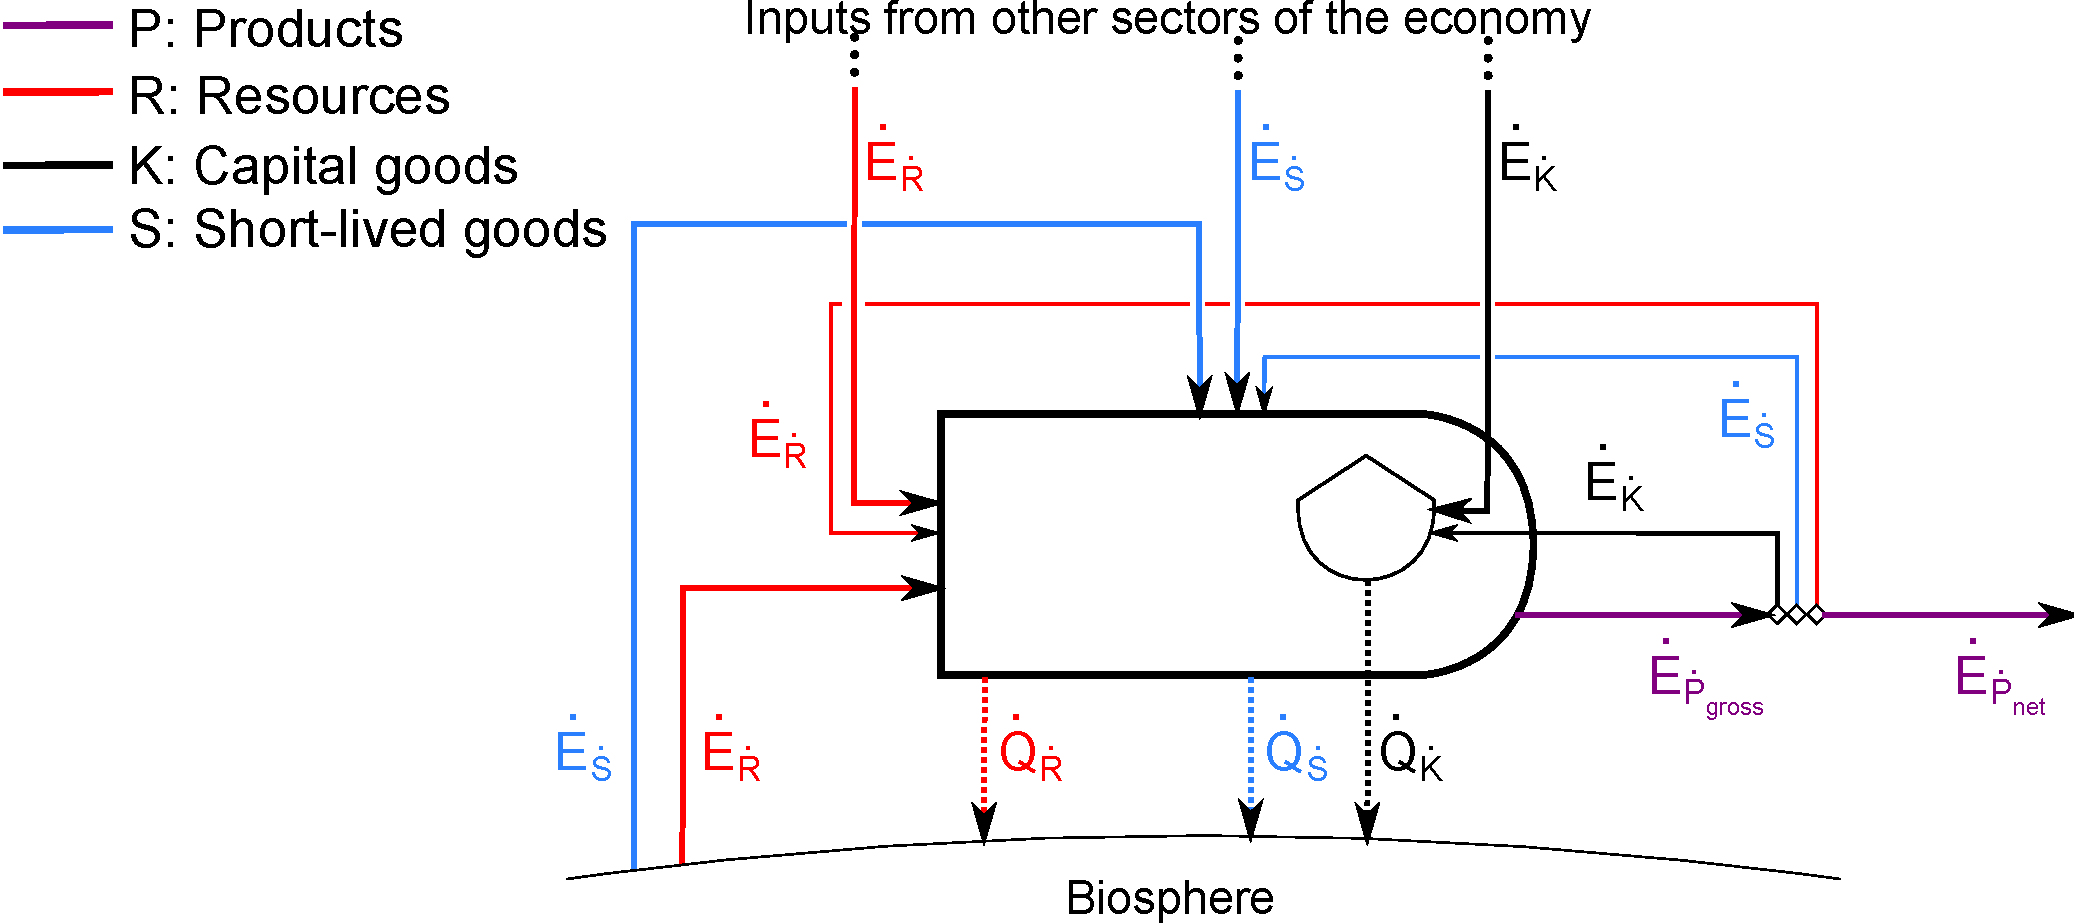
\includegraphics[width=0.8\linewidth]{Part_1/Chapter_Energy/images/PERKS_basic_unit_energy_content.pdf}
\caption[Energy content of material flows for a single sector]{Energy content ($\dot{E}$) of material flows 
($\dot{R}$, $\dot{S}$, and $\dot{K}$) 
from Figure~\ref{fig:PERKS_materials}.}
\label{fig:PERKS_energy_content}
\end{figure}

For any boundary (around, say, a machine, a plant,
a sector of the economy, or the entire economy itself), 
the First Law of Thermodynamics says that 
the accumulation rate 
of direct energy within the 
boundary $\left( \frac{\mathrm{d}E}{\mathrm{d}t} \right)$
is equal to the sum of the incoming and outgoing direct energy transfer 
rates ($\dot{E}$)
less outflowing energy carried by wastes 
($\dot{Q}_{out}$). 
Energy is conserved: it be neither created nor destroyed.
%
\begin{equation} \label{eq:First_Law_with_accumulation}
	\frac{\mathrm{d}E}{\mathrm{d}t} = \sum \dot{E} - \sum \dot{Q}_{out}
\end{equation}

When there is no accumulation of direct energy within the boundary
$\left( \frac{\mathrm{d}E}{\mathrm{d}t} = 0 \right)$, the sum of all 
signed direct energy flow rates ($\dot{E}$) 
and waste heats ($\dot{Q}_{out}$) will be zero.
%%
\begin{equation} \label{eq:First_Law_no_accumulation}
	0 = \sum \dot{E} - \sum \dot{Q}_{out}
\end{equation}

It is important to note that the direct energy associated with some material flows can
be so small as to be negligible compared to other direct energy flows in the economy.
For example, there is a small amount of chemical energy in steel that could be
released upon combustion. 
However, the direct energy associated with flows of steel within the economy
is almost negligible. (The \emph{embodied} energy of the steel is most certainly
\emph{not} negligible, as will be discussed in Chapter~\ref{chap:embodied_energy}.)
On the other hand, the direct energy flow rates for 
fossil fuels
(coal, oil, and natural gas)
are typically orders of magnitude larger than any other 
material flows due to large chemical potential energy content.

To simplify the direct energy analysis, 
we can aggregate the direct energy flows of Figure~\ref{fig:PERKS_energy_content}
into single arrows when appropriate. 
For example, the direct energy inputs from other sectors of the economy
(labeled as $\dot{E}_{\dot{R}}$, $\dot{E}_{\dot{S}}$, and $\dot{E}_{\dot{K}}$ 
at the top of Figure~\ref{fig:PERKS_energy_content}) can be summed to $\dot{E}$ 
(in Figure~\ref{fig:PERKS_energy}) such that
%
\begin{equation} \label{eq:direct_energy_aggregation}
	\dot{E} 
	= \dot{E}_{\dot{R}} 
	+ \dot{E}_{\dot{S}} 
	+ \dot{E}_{\dot{K}}.
\end{equation}

\begin{figure}[!ht]
\centering
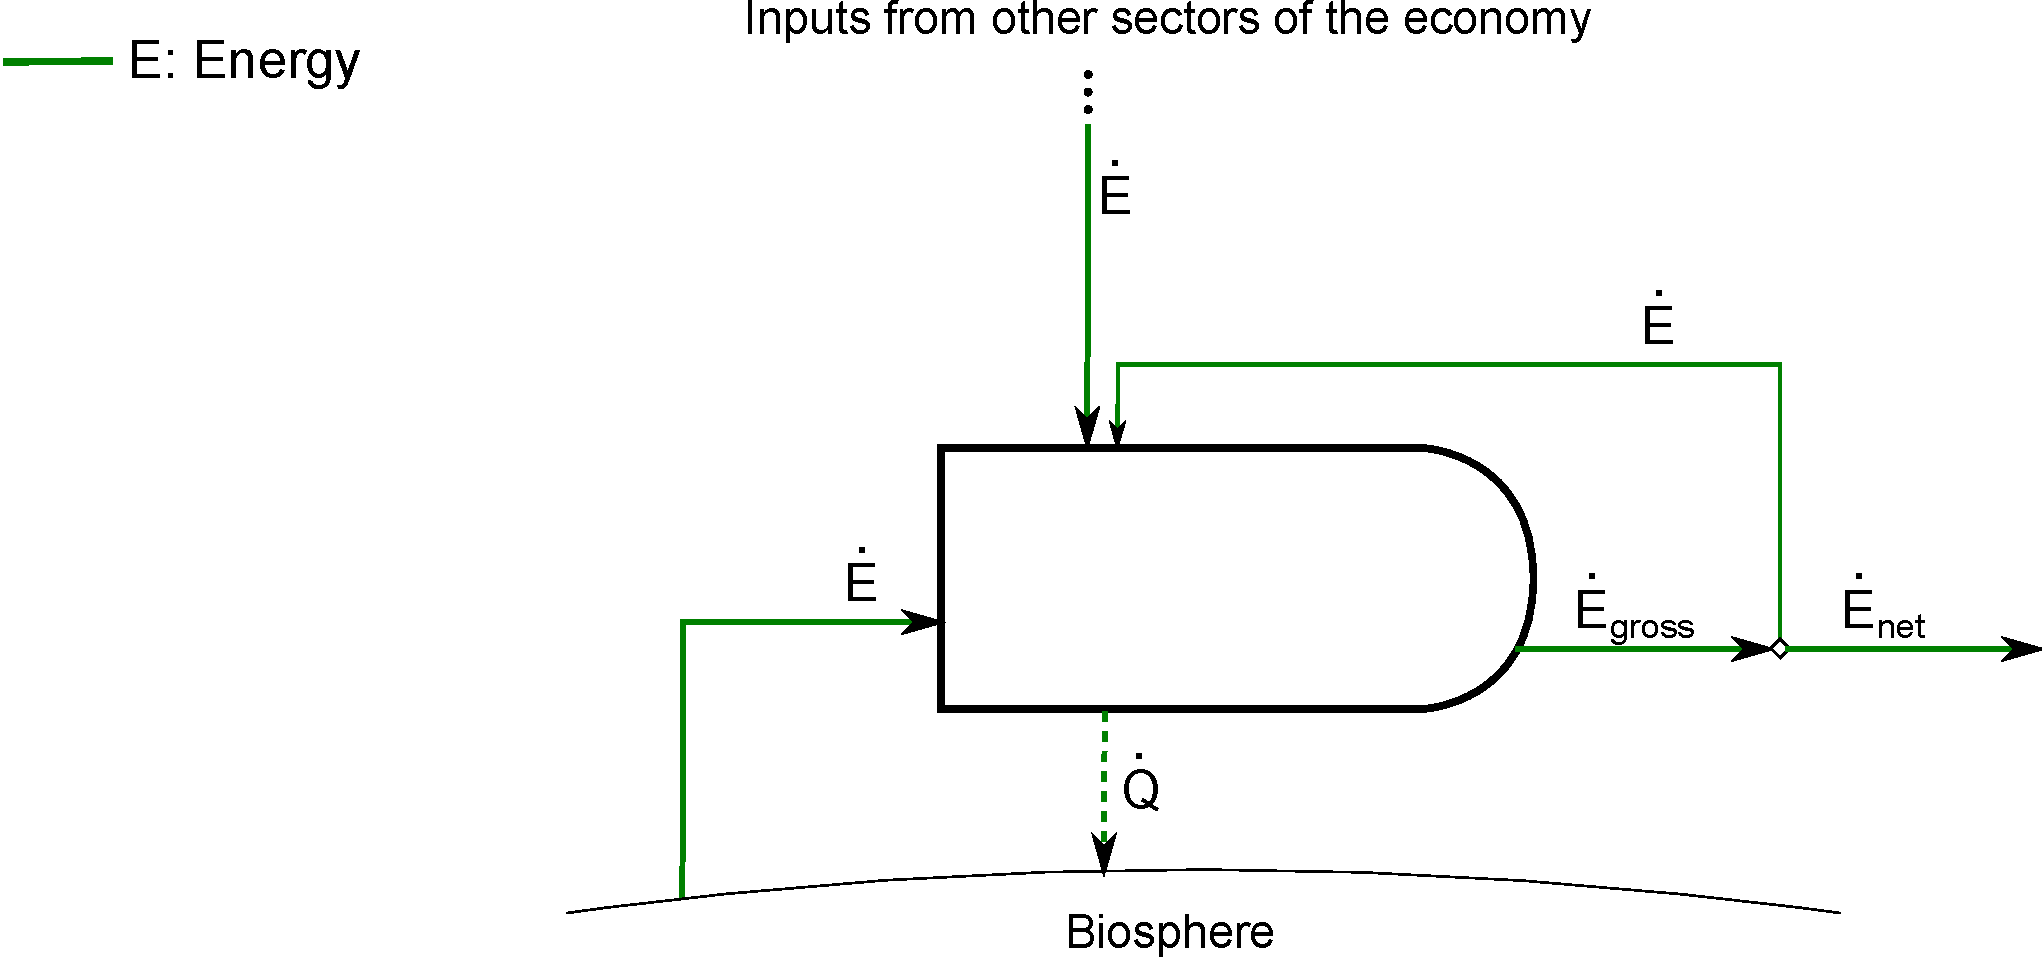
\includegraphics[width=\linewidth]{Part_1/Chapter_Energy/images/PERKS_basic_unit_energy.pdf}
\caption[Aggregated direct energy flows for a single sector]{Aggregated direct energy flows ($\dot{E}$) around 
the producer of Figure~\ref{fig:PERKS_energy_content}.}
\label{fig:PERKS_energy}
\end{figure}


%%%%%%%%%% Energy: Example A %%%%%%%%%%
\section{Example A: single-sector economy} % chktex 13
\label{sec:A_energy}
%%%%%%%%%%

Aggregated direct energy flows are now applied to Example A, 
the single-sector economy shown in Figure~\ref{fig:A_materials}.
By summing the direct energy flows associated with
each material flow of Figure~\ref{fig:A_materials}, we obtain
a simplified picture of direct energy flows in the economy,
as shown in Figure~\ref{fig:A_energy}.

\begin{landscape}
\begin{figure}[!ht]
\centering
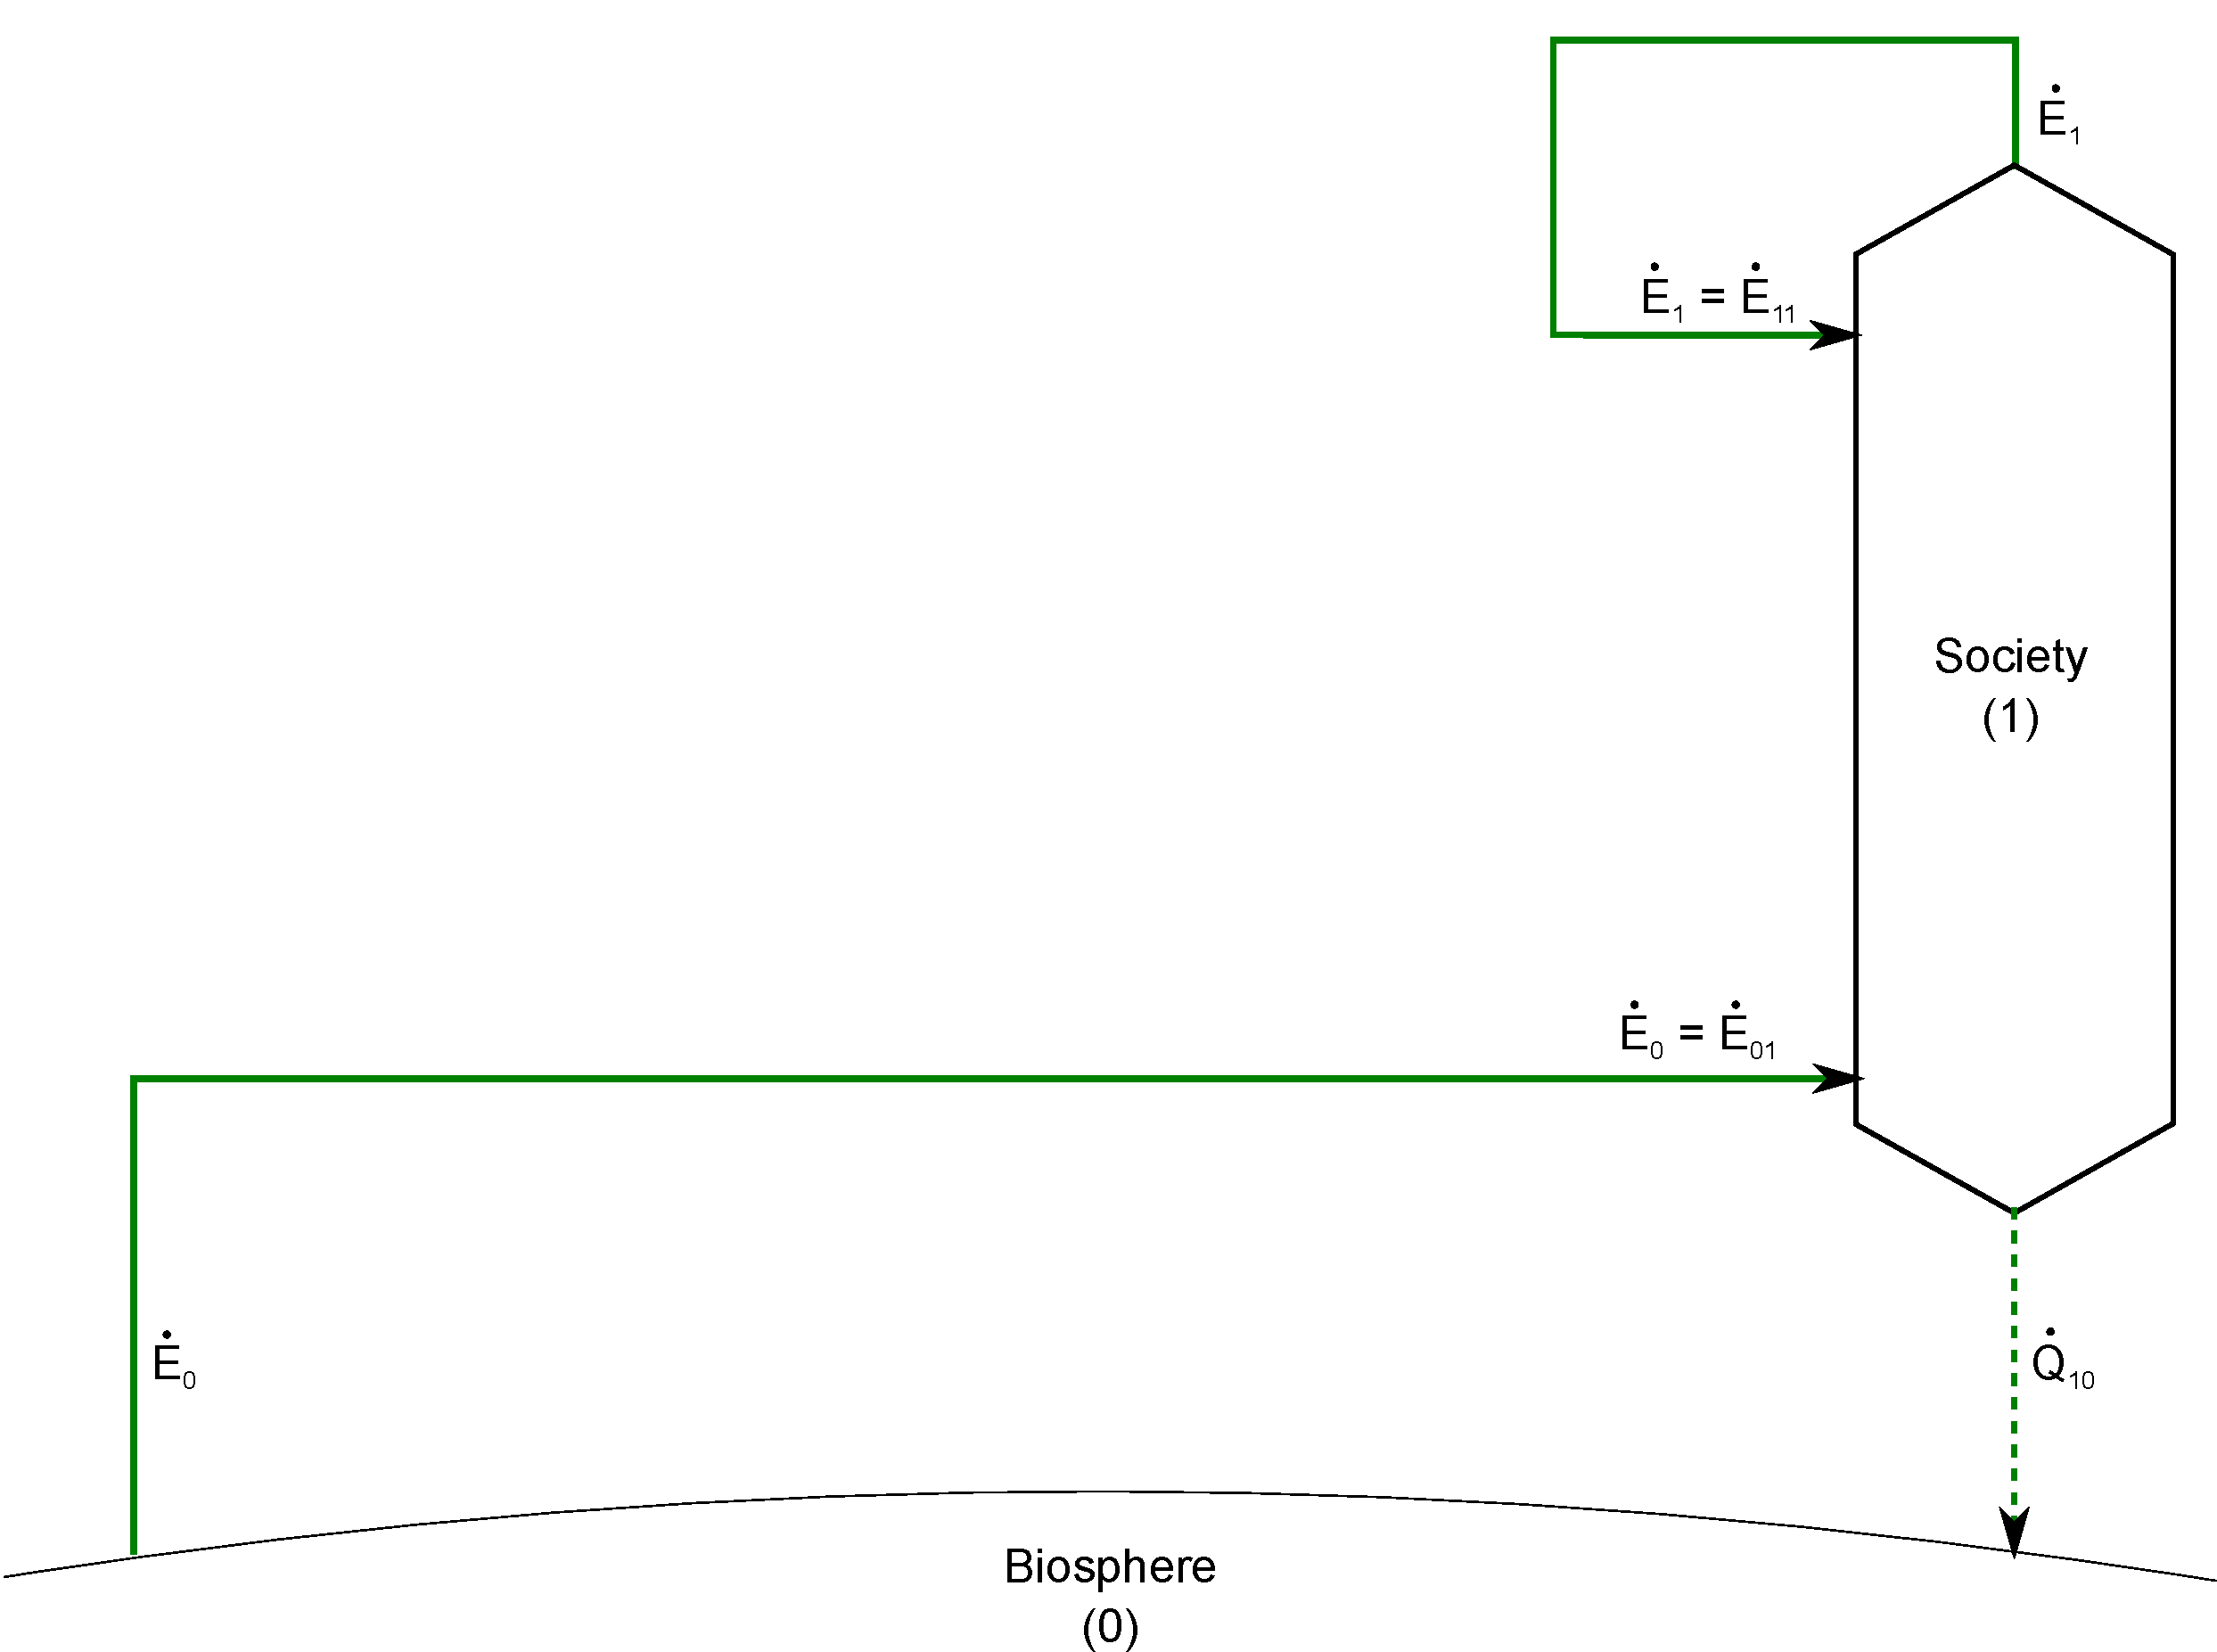
\includegraphics[width=0.8\linewidth]{Part_1/Chapter_Energy/images/1_sector_direct_energy.pdf}
\caption[Direct energy flows a one-sector economy]{Direct energy flows ($\dot{E}$) a one-sector economy.}
\label{fig:A_energy}
\end{figure}
\end{landscape}

We distinguish useful direct energy inputs to a sector of the economy
($\dot{E}_{01}$ in Figure~\ref{fig:A_energy}) from wasteful direct energy flows 
($\dot{Q}_{10}$ in Figure~\ref{fig:A_energy}), 
because $\dot{Q}$ typically denotes thermal energy, 
and most waste energy is in the form of thermal
energy, i.e., waste heat. In Figure~\ref{fig:A_energy}, direct energy input to the 
economy ($\dot{E}_{01}$) is shown as being extracted from the biosphere, because
the vast majority of direct energy today is derived from fossil fuels.
Waste heat from the economy ($\dot{Q}_{10}$) is shown as returning 
to the biosphere.

As discussed in Section~\ref{sec:energy_methodology}, 
both direct energy ($\dot{E}$), and waste heat ($\dot{Q}$) 
are accounted by the First Law of Thermodynamics. 
Accounting for possible accumulation of direct energy, 
the First Law of Thermodynamics for Example~A indicates that
%
\begin{equation} \label{eq:dE_0/dt_single_sector}
	\frac{\mathrm{d}E_0}{\mathrm{d}t} 
	= \dot{Q}_{10} 
	- \dot{E}_{01}
\end{equation}
%
and
%
\begin{equation} \label{eq:dE_1/dt_single_sector}
	\frac{\mathrm{d}E_{1}}{\mathrm{d}t} 
	= \dot{E}_{01} 
	+ \dot{E}_{11}
	- \dot{E}_{1}
	- \dot{Q}_{10}.
\end{equation}

Note that $\dot{E}_{1}$ is the gross direct energy production rate
of society. 
For example, firms extract crude oil from the biosphere (a component of $\dot{E}_{01}$) 
and refine it into petroleum products 
(which in Figure~\ref{fig:A_energy}, leave as part of flow $\dot{E}_{1}$)
that are then consumed by society.
The direct energy consumption of extraction and refining firms 
is a component of $\dot{E}_{11}$,
that is some of the energy that circulates back into society in flow $\dot{E}_{11}$
is used within the extraction and refining processes to generate flow
$\dot{E}_{01}$ from the biosphere.

Aside from, for example, the US 
Strategic Petroleum Reserve, 
we are not stockpiling oil and coal at any meaningful rate, 
i.e.\ we consume fossil fuels at a rate equal to their extraction rate. 
Thus, the world is not accumulating direct energy 
in the economy.\footnote{A counter-example could be made 
for nuclear fuels where ``spent'' fuel represents a large exergetic stockpile. 
However, this reserve is not (presently) economically useful.} 
(The world \emph{is}, however, 
accumulating \emph{embodied} energy
in the economy as we shall see 
in Chapter~\ref{chap:embodied_energy}.) 
Thus, the accumulation rates for direct energy 
$\left( \frac{\mathrm{d}E}{\mathrm{d}t} \right)$ in the above equations 
could be set to zero as follows:
%
\begin{equation} \label{eq:biosphere_direct_energy_steady_state}
	0 
	= \dot{Q}_{10} 
	- \dot{E}_{01}
\end{equation}
%
and
%
\begin{equation} \label{eq:single_sector_direct_energy_steady_state}
	0 
	= \dot{E}_{01} 
	+ \dot{E}_{11}
	- \dot{E}_{1} 
	- \dot{Q}_{10}.
\end{equation}
%
However, we shall see later (in Chapter~\ref{chap:direct_energy}) 
that keeping direct energy accumulation terms
$\left( \frac{\mathrm{d}E}{\mathrm{d}t} \right)$ 
provides an advantage when deriving embodied energy accounting equations.


%%%%%%%%%% Energy: Example B %%%%%%%%%%
\section{Example B: two-sector economy} % chktex 13
\label{sec:B_energy}
%%%%%%%%%%

For Example~B, we split Production~(2) from 
Society~(1). Figure~\ref{fig:B_energy} shows aggregated
direct energy flows associated with the material flows of Figure~\ref{fig:B_materials}.

\begin{landscape}
\begin{figure}[!ht]
\centering
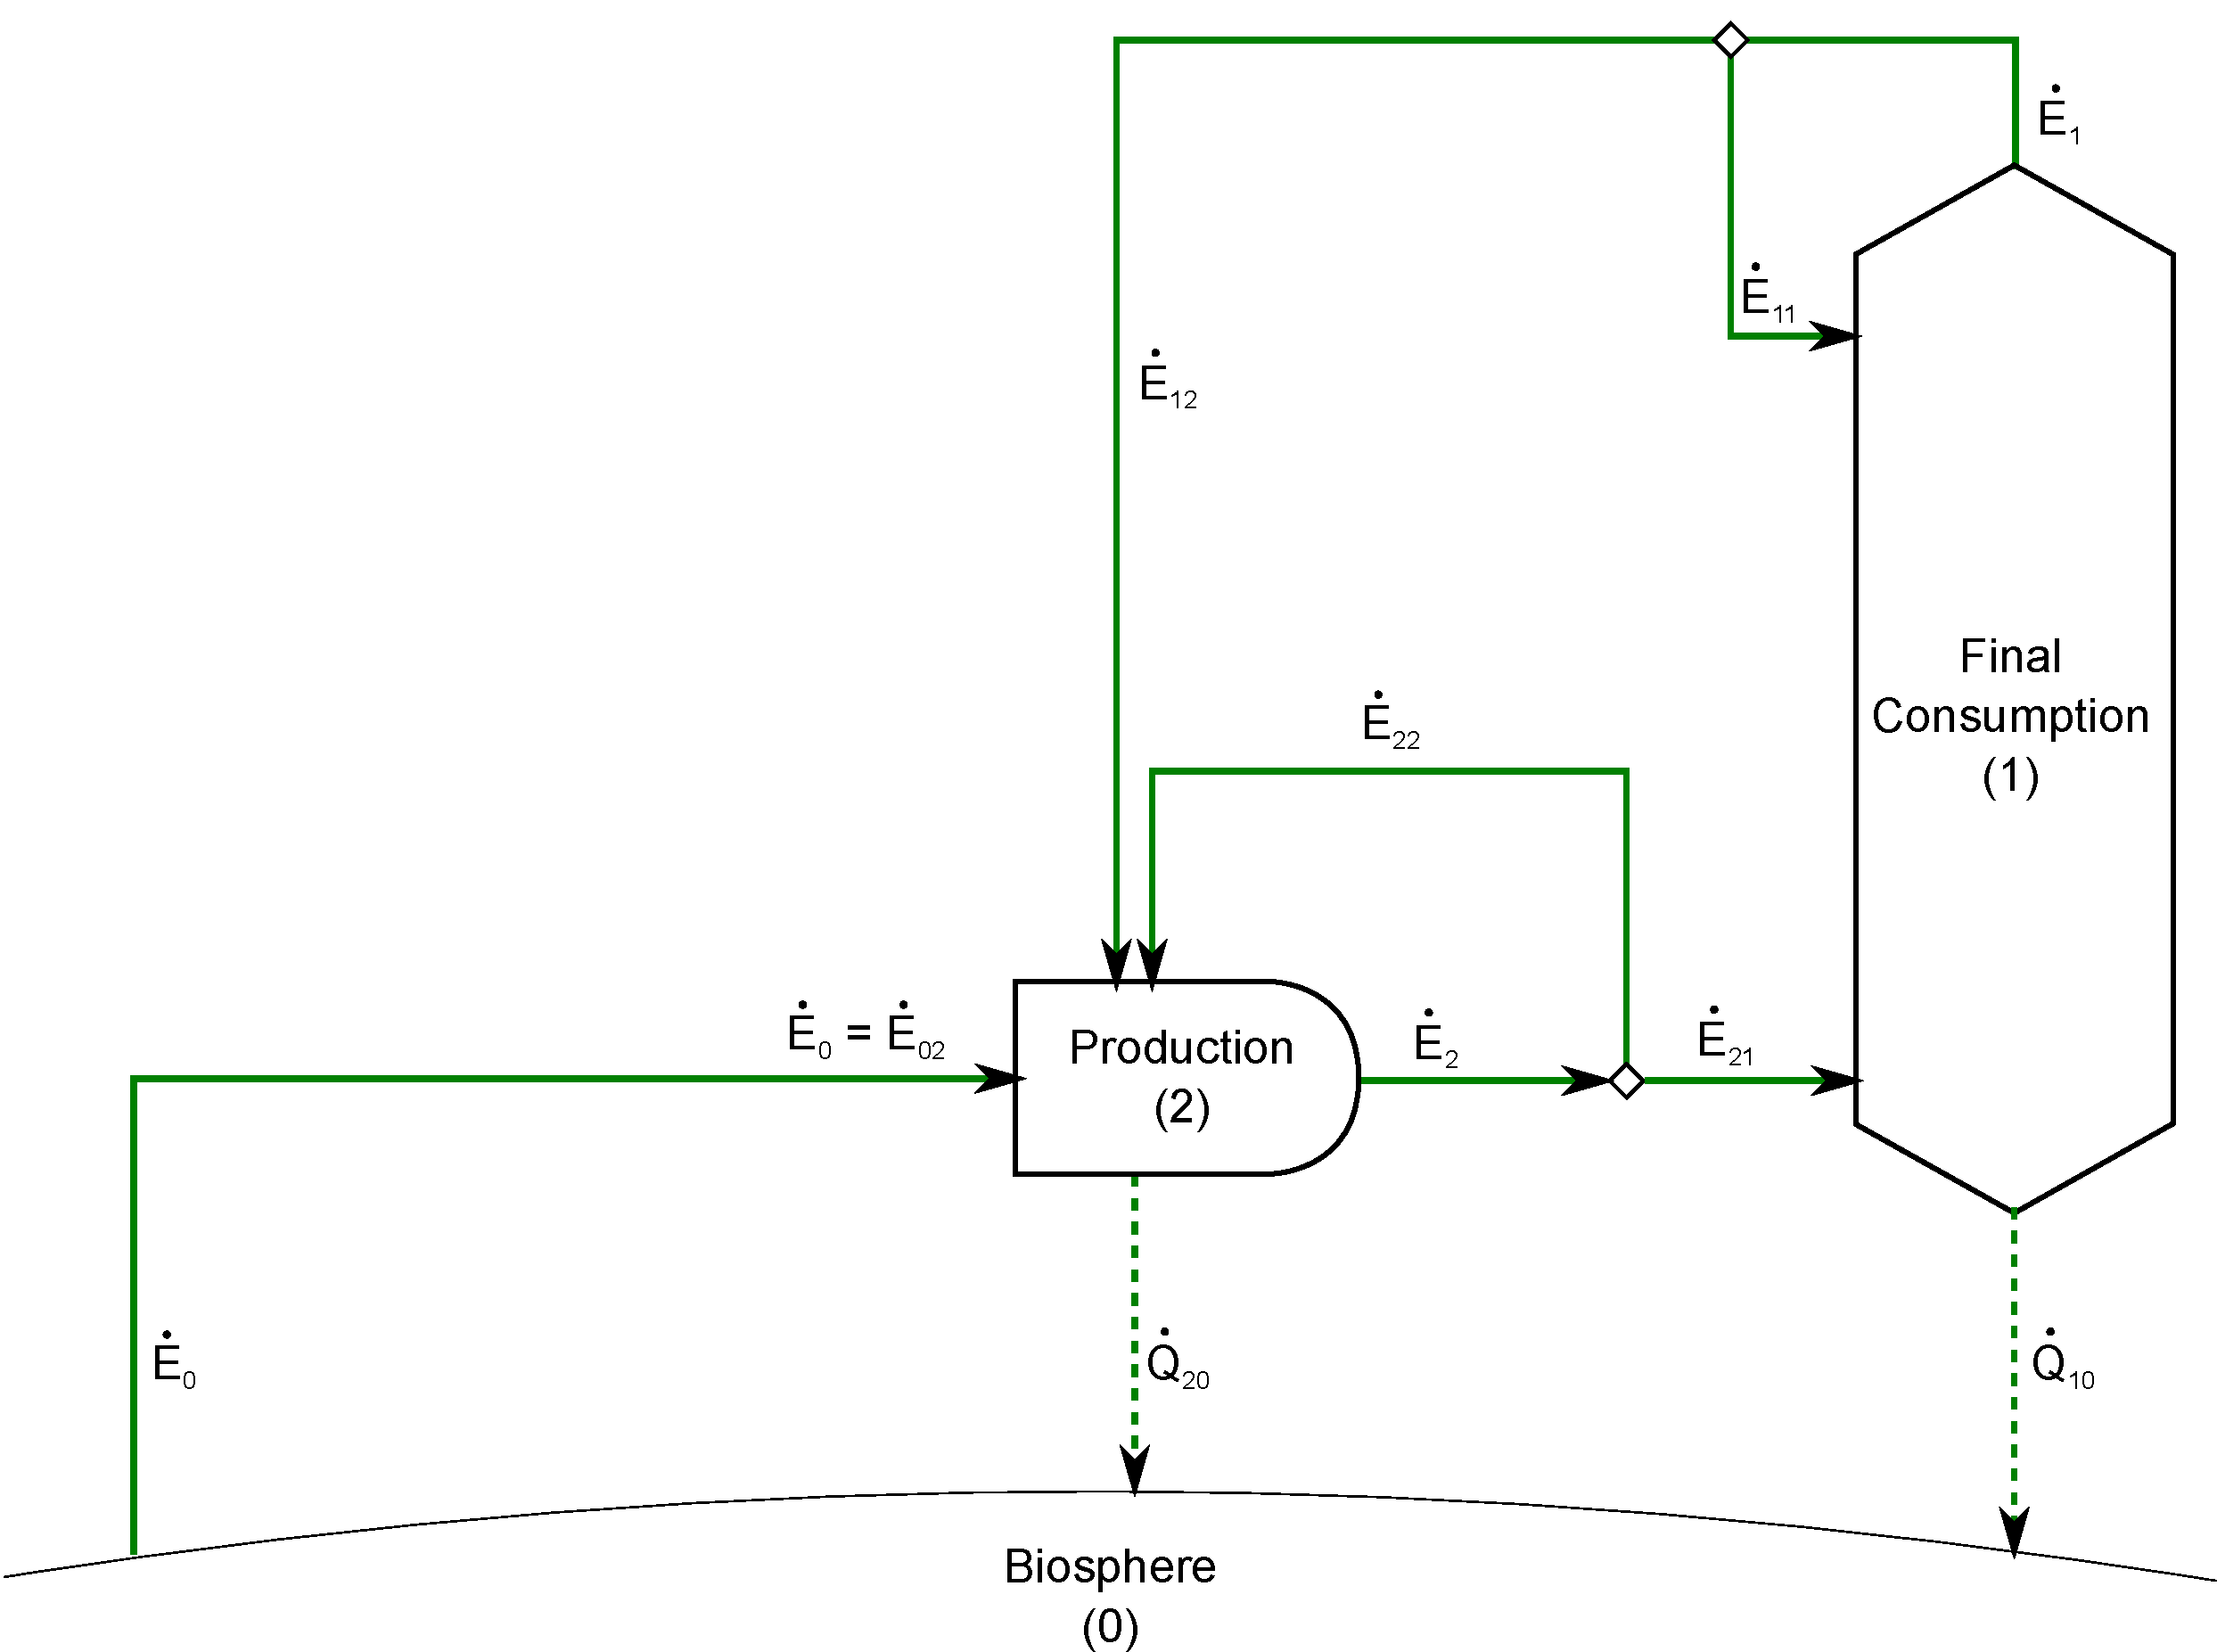
\includegraphics[width=0.8\linewidth]{Part_1/Chapter_Energy/images/2_sector_direct_energy.pdf}
\caption[Direct energy flows for a two-sector economy]{Direct energy flows ($\dot{E}$) for a two-sector economy.}
\label{fig:B_energy}
\end{figure}
\end{landscape}

The First Law of Thermodynamics
requires that both 
direct energy and 
waste heat
be conserved around each 
entity (1 and 2) as well as around the Biosphere~(0).

\noindent{}First Law energy accounting around the Biosphere~(0) and Society~(1) gives
%
\begin{equation} \label{eq:CV_E_dot_0}
	\frac{\mathrm{d}E_{0}}{\mathrm{d}t} 	 
	= \dot{Q}_{10} 
	+ \dot{Q}_{20} 
	- \dot{E}_{02},
\end{equation}
%
and 
%
\begin{equation} \label{eq:CV_E_dot_1}
	\frac{\mathrm{d}E_{1}}{\mathrm{d}t} 	 
	= \dot{E}_{11} 
	+ \dot{E}_{21}
	- \dot{E}_{1}
	- \dot{Q}_{10}.
\end{equation}

Note that $\dot{E}_{12}$ represents useful work that people
and draft animals contribute to Production (2). 
Ayres and Warr~\cite{Ayres:2003ec,Warr:2012cg} call this ``muscle work.'' 
$\dot{E}_{11}$ represents the muscle work required for consumption. 
Direct energy (electricity, oil, natural gas, etc.) 
required for consumption by final demand 
is included in $\dot{E}_{21}$.

The First Law around Production (2), 
including the accumulation rate of direct energy in the sector 
$\left(\frac{\mathrm{d}E_{2}}{\mathrm{d}t}\right)$, yields
%
\begin{equation} \label{eq:CV_E_dot_2}
	\frac{\mathrm{d}E_{2}}{\mathrm{d}t} 
	= \dot{E}_{02} 
	+ \dot{E}_{12}
	+ \dot{E}_{22} 
	- \dot{E}_{2} 
	- \dot{Q}_{20}.
\end{equation}
%
It is notable that Production (2) consumes ($\dot{E}_{22}$)
a portion of its gross energy output ($\dot{E}_2$): \emph{it takes energy to make energy}.
The gross direct energy production of the Energy sector~(2) is 
$\dot{E}_{2}$, and the direct energy consumption of the Energy sector~(2) is 
$\dot{E}_{12} + \dot{E}_{22}$. 
The net direct energy production Energy~(2)
is given by $\dot{E}_{2} - (\dot{E}_{12} + \dot{E}_{22})$.
The \emph{energy return on investment}
($EROI$)~\cite{Smith1960, Hall1986} of the Energy sector~(2) is given by
%
\begin{equation} \label{eq:C-EROI}
	EROI_{2} 
	= \frac{\dot{E}_{2}}{\dot{E}_{12} + \dot{E}_{22}}.
\end{equation}
%
EROI represents the energy production \emph{per unit} of energy
invested by society in the production process and may
be considered a measure of the ease of obtaining
energy resources from the biosphere.
Although the definition of EROI, as outlined here, 
is easy to articulate 
$\left( \mathrm{essentially,} \: \frac{\mathrm{energy~out}}{\mathrm{energy~in}} \right)$,
the EROI calculation involves a multitude of system boundary considerations.
These issues are well covered by both Murphy, et al.~\cite{Murphy2011}
and Brandt, et al.~\cite{Brandt2011a, Brandt2013} who outline varying
EROI	ratios according to what factors are included in the calculation.
Because we are dealing only with direct energy in this chapter
(and not upstream energy embodied in materials),
the EROI defined here is EROI$_{2,d}$~\cite[Table~1]{Murphy2011}
or GER$_{\gamma}$~\cite[Table~1]{Brandt2011},
where GER stands for \emph{gross energy ratio}
an equivalent metric to EROI\@.

As discussed in Chapter~\ref{chap:materials},
society relies heavily on concentrations of high quality
material resources.
As we mine lower quality material resources we require
larger inputs of energy both directly,
to process greater volumes of material,
but also indirectly to build the extra capital equipment
necessary to do the processing.
The same is also true of energy resources within the environment.
Fossil fuels represent stocks of solar energy
accumulated (in the form of biomass)
over many millions of years.
These resources are extremely far from equilibrium with the environment.
EROI can be considered an indicator of energy resource quality.
As EROI (and thus energy quality) declines,
more energy is needed to extract and deliver energy from the environment,
both directly, for example the energy to pump oil from deeper underground,
and indirectly, in order to build the extra oil rigs necessary to 
maintain production levels.%
	\footnote{
	This issue 
	of resource quality will be re-visited in 
	Chapters~\ref{chap:embodied_energy}~and~\ref{chap:value}
	and discussed in more
	detail in Section~\ref{sec:resource_quality_and_irreversibility}.
	}

Equation~\ref{eq:CV_E_dot_0} can be generalized with a sum as
%
\begin{equation} \label{eq:CV_E_biosphere_general}
	\frac{\mathrm{d}E_{0}}{\mathrm{d}t} 
	= \sum\limits_{i=1}^n \left( \dot{Q}_{i0} - \dot{E}_{0i} \right),
\end{equation}
%
where $n$ is the number of economic sectors in the accounting framework
(in this example, $n = 2$).
Similarly, Equations~\ref{eq:CV_E_dot_1}~and~\ref{eq:CV_E_dot_2} 
can generalized with a sum as
%
\begin{equation} \label{eq:B-CV_E_econ_general}
	\frac{\mathrm{d}E_{j}}{\mathrm{d}t} 
	= \sum\limits_{i=0}^n\dot{E}_{ij} 
	- \dot{E}_{j}  
	- \dot{Q}_{j0},
\end{equation}
%
where $j \in [1, n]$.


%%%%%%%%%% Energy: Example C %%%%%%%%%%
\section{Example C: three-sector economy} % chktex 13
\label{sec:C_energy}
%%%%%%%%%%

We can extend Example~B, to include an Energy sector~(2) 
and a Goods and Services sector~(3), thereby obtaining
a fuller picture of direct energy flows among sectors
(Figure~\ref{fig:C_energy}).

\begin{landscape}
\begin{figure}[!ht]
\centering
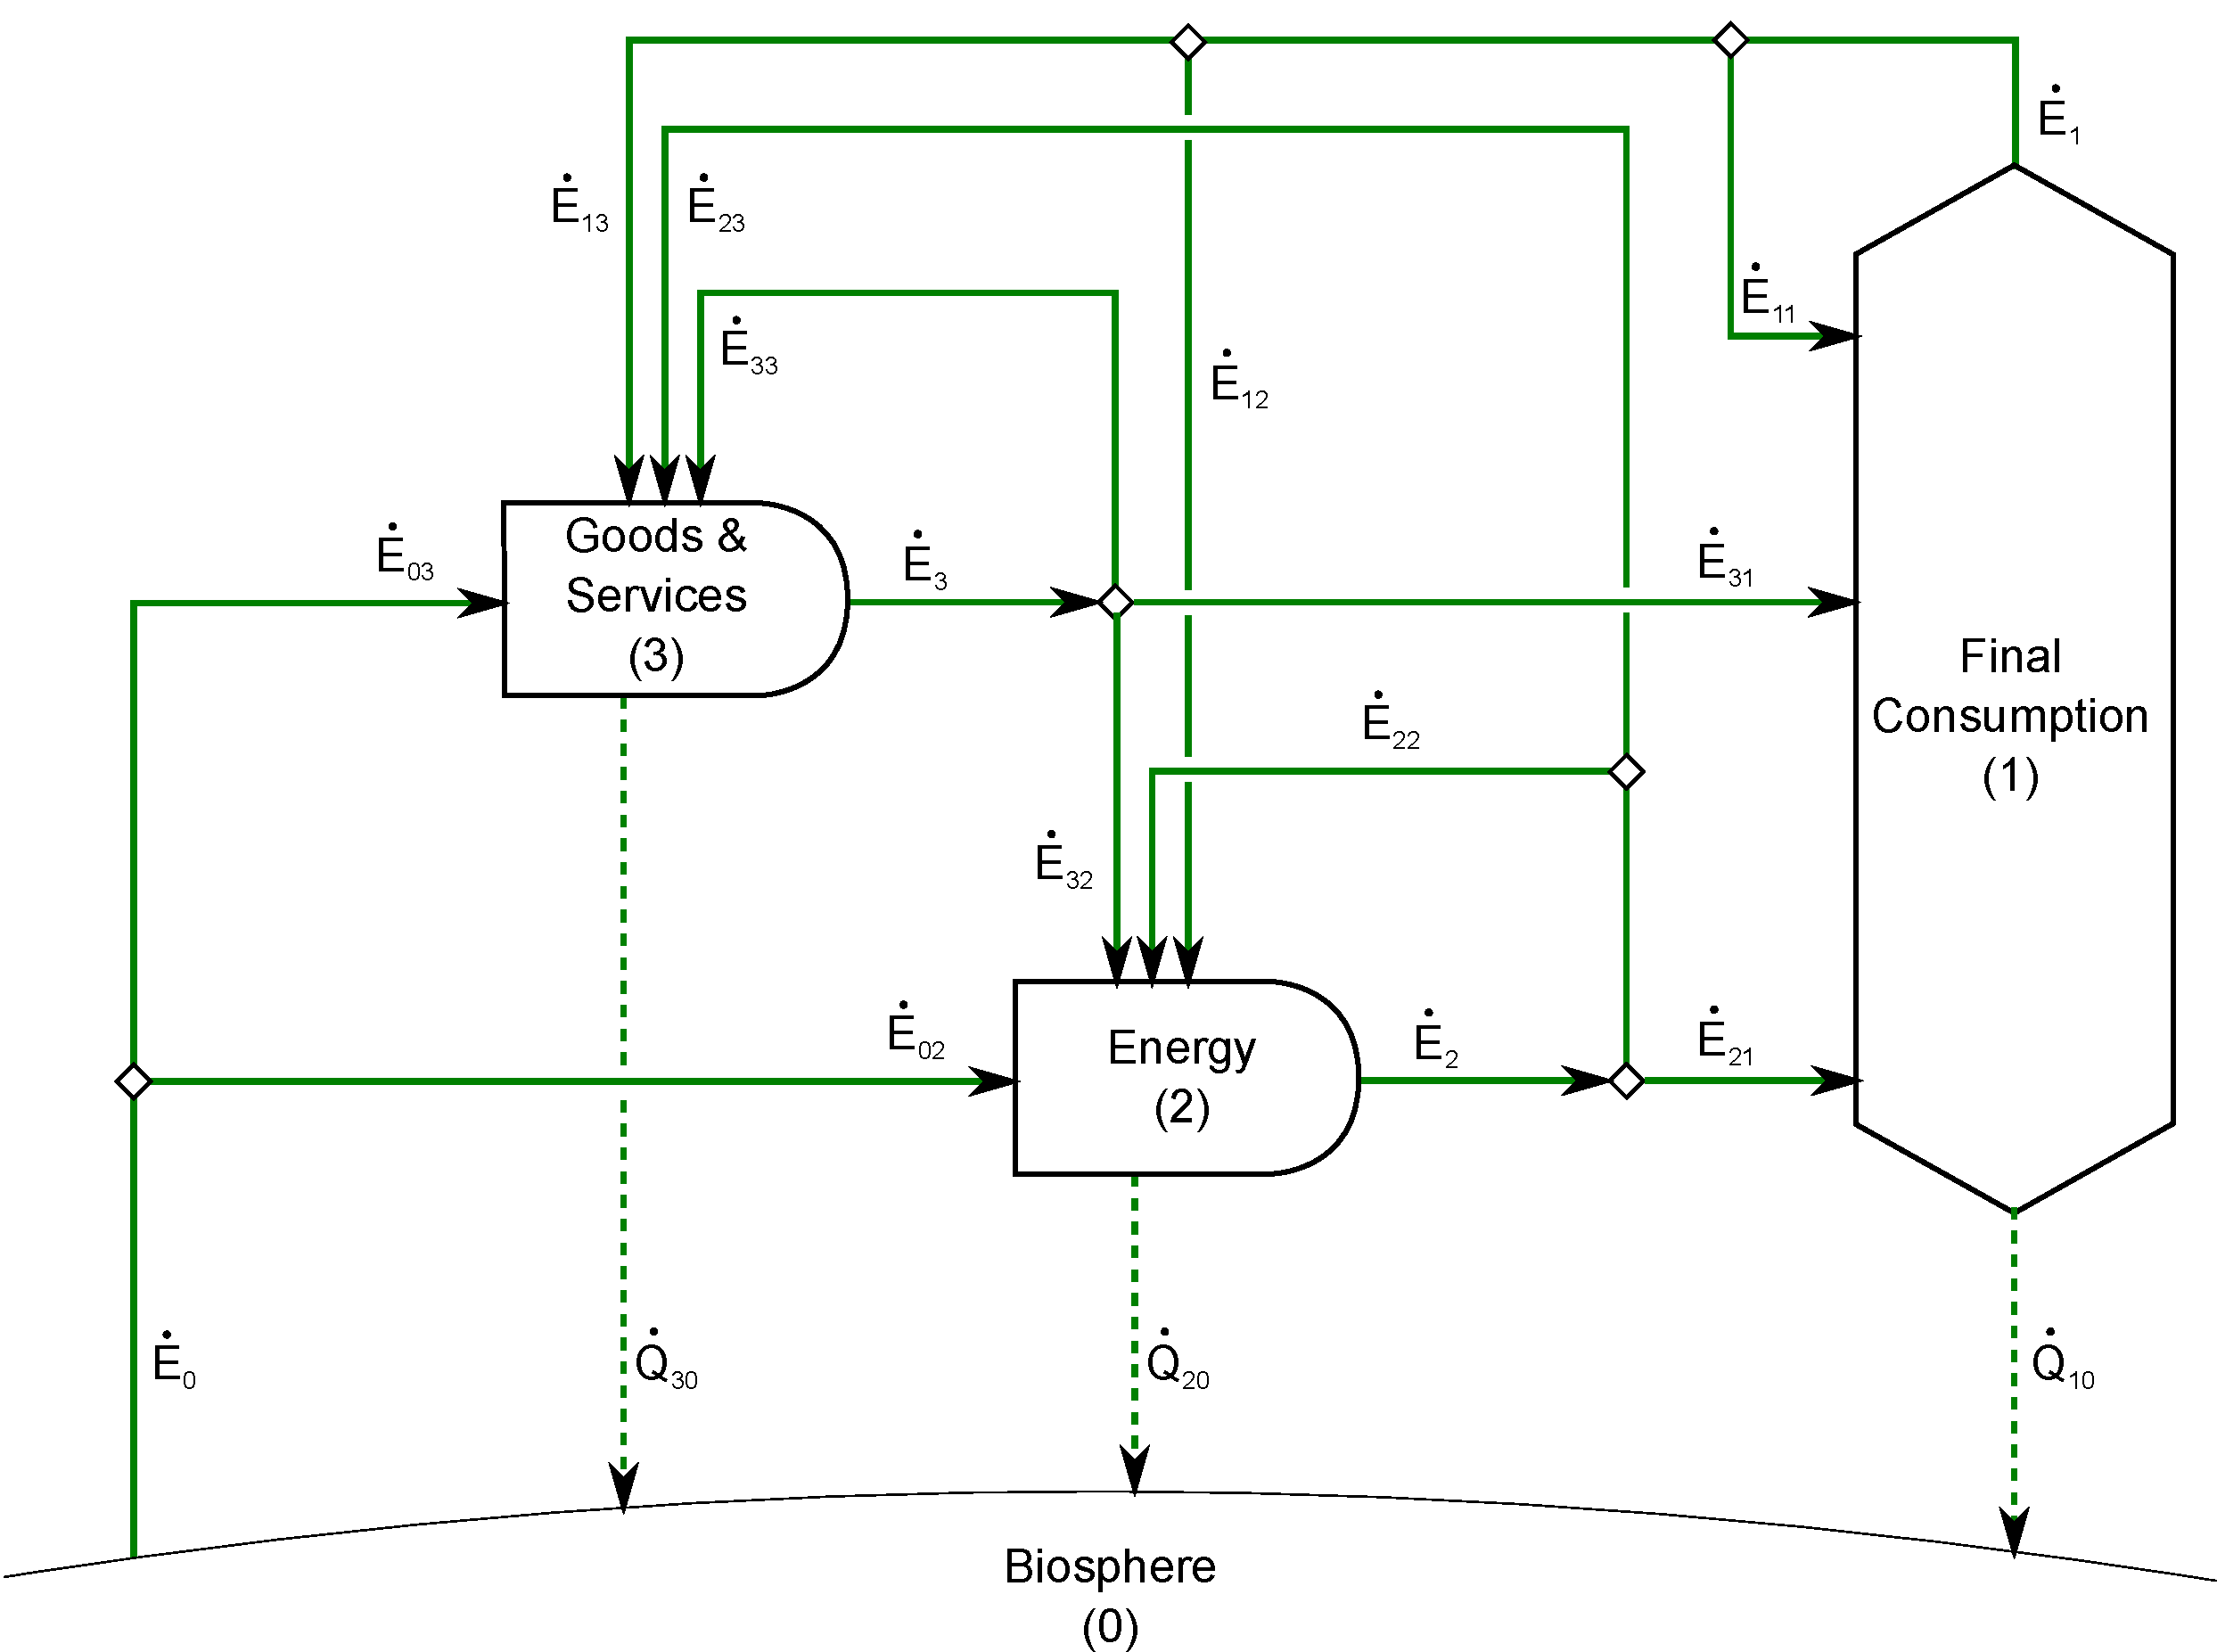
\includegraphics[width=0.8\linewidth]{Part_1/Chapter_Energy/images/3_sector_direct_energy.pdf}
\caption[Direct energy flows for a three-sector economy]{Direct energy flows ($\dot{E}$) for a three-sector economy.}
\label{fig:C_energy}
\end{figure}
\end{landscape}

The First Law of Thermodynamics applied to the 
Biosphere~(0), Society~(1), and the Energy~(2) gives
%
\begin{equation} \label{eq:C-CV_E_dot_0}
	\frac{\mathrm{d}E_{0}}{\mathrm{d}t} 	 
	= \dot{Q}_{10} 
	+ \dot{Q}_{20} 
	+ \dot{Q}_{30} 
	- \dot{E}_{02} 
	- \dot{E}_{03},
\end{equation}
%
\begin{equation} \label{eq:C-CV_E_dot_1}
	\frac{\mathrm{d}E_{1}}{\mathrm{d}t}
	= \dot{E}_{11}
	+ \dot{E}_{21}  
	+ \dot{E}_{31} 
	- \dot{E}_{1}
	- \dot{Q}_{10},
\end{equation}
%
and 
%
\begin{equation} \label{eq:C-CV_E_dot_2}
	\frac{\mathrm{d}E_{2}}{\mathrm{d}t} 	 
	= \dot{E}_{02} 
	+ \dot{E}_{12}
	+ \dot{E}_{22} 
	+ \dot{E}_{32} 
	- \dot{E}_{2} 
	- \dot{Q}_{20}.
\end{equation}

The First Law applied to the Goods and Services sector~(3) including, 
for now, the accumulation rate of direct energy in the sector 
$\left(\frac{\mathrm{d}E_{3}}{\mathrm{d}t}\right)$ yields
%
\begin{equation} \label{eq:C-CV_E_dot_3}
	\frac{\mathrm{d}E_{3}}{\mathrm{d}t} 
	= \dot{E}_{03} 
	+ \dot{E}_{13}
	+ \dot{E}_{23} 
	+ \dot{E}_{33} 
	- \dot{E}_3 
	- \dot{Q}_{30}.
\end{equation}

Similar to Example~B, we can generalize 
Equations~\ref{eq:C-CV_E_dot_0}--\ref{eq:C-CV_E_dot_3}
with sums to obtain
%
\begin{equation} \label{eq:C-CV_E_biosphere_general}
	\frac{\mathrm{d}E_{0}}{\mathrm{d}t} 	 
	= \sum\limits_{i=1}^n \dot{Q}_{i0} - \sum\limits_{i=1}^n \dot{E}_{0i}
\end{equation}
%
and
%
\begin{equation} \label{eq:C-CV_E_econ_general}
	\frac{\mathrm{d}E_{j}}{\mathrm{d}t} 
	= \sum\limits_{i=0}^n\dot{E}_{ij} 
	- \dot{E}_{j}  
	- \dot{Q}_{j0},
\end{equation}
%
where $j \in [1, n]$. 
Equations~\ref{eq:C-CV_E_biosphere_general} and 
\ref{eq:C-CV_E_econ_general} are identical to 
Equations~\ref{eq:CV_E_biosphere_general} and 
\ref{eq:B-CV_E_econ_general}, 
indicating that we have successfully generalized 
the framework to any number of sectors.

In this economy, the purpose of Goods and Services~(3) 
is to produce goods and provide services, 
it provides no direct energy to society. 
The purpose of Energy~(2) is to make direct energy ($\dot{E}$) 
available to the economy and society in a useful form.
We may simplify the above equations
by realizing that (a)~$\dot{E}_{3} = \dot{E}_{3i} = 0$, 
because Goods and Services~(3)
is assumed to produce no direct energy, 
and (b) $\dot{E}_{03} = 0$, 
because Goods and Services~(3) 
receives no direct energy from the Biosphere~(0), 
except via the Energy sector~(2).
Thus, several terms in the sums of
Equation~\ref{eq:C-CV_E_econ_general}
will be zero.


%%%%%%%%%% Energy: Auto industry example %%%%%%%%%%
\section{Direct energy in the auto industry}
\label{sec:energy_auto}
%%%%%%%%%%

In this section we discuss inflow of direct energy into the automobile industry
as shown in Figure~\ref{fig:PERKS_energy_auto}.
In 2010, the automobile industry purchased 28 trillion kJ of total energy from all sources. 
Table~\ref{tab:auto_energy} shows the breakdown of energy by source. 

\begin{figure}[!ht]
\centering
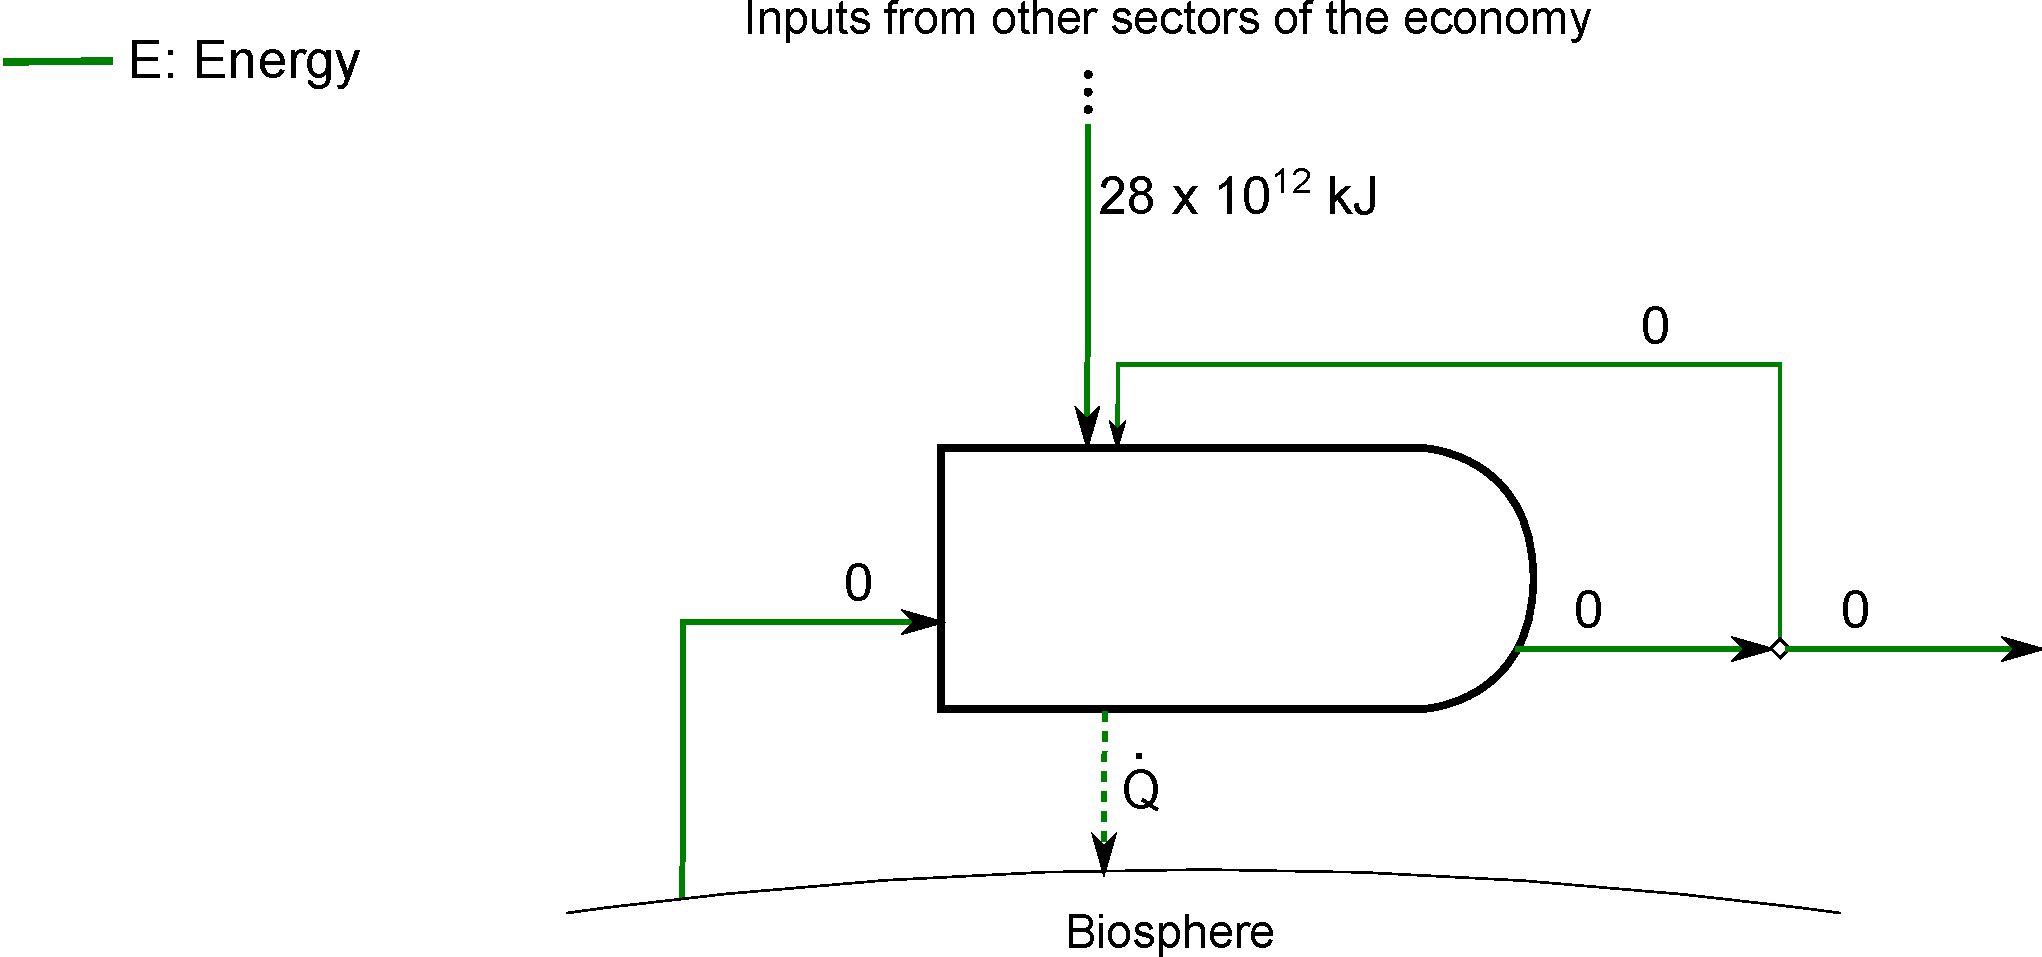
\includegraphics[width=\linewidth]{Part_1/Chapter_Energy/images/PERKS_basic_unit_energy_auto_ind.pdf}
\caption[Direct energy flows for the US automobile industry]
{Direct energy flows for the US automobile industry.\cite[Table 7.6]{EIA:2014aa}}
\label{fig:PERKS_energy_auto}
\end{figure}

\begin{table}
\caption[Energy inputs to US auto industry in 2010]{Energy inputs to US auto industry 
(NAICS Code 336111) in 2010.\cite[Table 7.6]{EIA:2014aa}}
\begin{center}
 \begin{tabular}{ r @{\hspace{2em}} l @{\hspace{2em}} l }
\toprule 
Source 			&		Quantity											&	Energy content [kJ]						\\
\midrule
Electricity 	&		$3.0 \times 10^{9}$ kW-hr   			&	$10.8 \times 10^{12}$ $^{a}$		\\
Natural gas 	&		$1.5 \times 10^{10}$  ft$^{3}$		&	$16.3 \times 10^{12}$				\\
Other       	&		$1.0 \times 10^{12}$  BTU				&	$1.1 \times 10^{12}$					\\
\midrule
Total       		&		\multicolumn{2}{l}{$2.8 \times 10^{13}$ kJ (thermal equivalent)}			 \\
\bottomrule
\multicolumn{3}{l}{{\footnotesize $^{a}$ Non-quality corrected value}}
\end{tabular}
\end{center}
\label{tab:auto_energy}
\end{table}

Total energy use can also be estimated by summing the energy use of the 
underlying detailed processes in manufacturing automobiles. 
Sullivan et al.\ arrive at an estimate of the ``gate-to-gate'' energy
used in the process of creating one automobile (the direct energy used within the
automobile manufacturing process only).\cite{Sullivan2010} 
This estimate can be
mulitplied by the number of vehicles manufactured in a given year 
to obtain total energy use by the 
automobile industry. 
Sullivan estimated a total direct energy use of 34,000 MJ for a generic 1,532 kg vehicle. 
% Using Sullivan's estimate in conjunction with the 19 trillion kJ of total auto industry energy use would suggest that there were
% approximately 560,000 vehicles produced in the US in 2010. (19 million GJ divided by 34 GJ).  That is at least in the ballpark of the estimated 2.7 million actual vehicles produced in 2010.\cite{Motor-Vehicle-Manufacturers-OICA:2014aa}


%%%%%%%%%%  Energy: Summary %%%%%%%%%%
\section{Summary}
\label{sec:energy_summary}
%%%%%%%%%%

In this chapter, we have developed equations, 
assisted by the First Law of Thermodynamics,
that describe the flow of 
direct energy ($\dot{E}$) through economies (Section~\ref{sec:energy_methodology}).
Examples~A--C afforded the opportunity to apply the equations to % chktex 8
analyze economies with increasing levels of disaggregation
(Sections~\ref{sec:A_energy}--\ref{sec:C_energy}). 
Finally, the energy flows for our running example, the US auto industry,
were discussed in Section~\ref{sec:energy_auto}.

In the next chapter, the direct energy equations developed above will be used to 
develop \emph{embodied} energy accounting equations for Examples~A--C. % chktex 8


\bibliographystyle{unsrt}
\bibliography{../../Metabolic}




% subsection subsection_name (end)


% Always give a unique label
% and use \ref{<label>} for cross-references
% and \cite{<label>} for bibliographic references
% use \sectionmark{}
% to alter or adjust the section heading in the running head
%% Instead of simply listing headings of different levels we recommend to let every heading be followed by at least a short passage of text. Furtheron please use the \LaTeX\ automatism for all your cross-references and citations.

%% Please note that the first line of text that follows a heading is not indented, whereas the first lines of all sequent paragraphs are.

%% Use the standard \verb|equation| environment to typeset your equations, e.g.
%
%% \begin{equation}
%% a \times b = c\;,
%% \end{equation}
%
%% however, for multiline equations we recommend to use the \verb|eqnarray|
%% environment\footnote{In physics texts please activate the class option \texttt{vecphys} to depict your vectors in \textbf{\itshape boldface-italic} type - as is customary for a wide range of physical jects.}.
%% \begin{eqnarray}
%% a \times b = c \nonumber\\
%% \vec{a} \cdot \vec{b}=\vec{c}
%% \label{eq:01}
%% \end{eqnarray}

%% \section{section Heading}
%% \label{sec:2}
%% Instead of simply listing headings of different levels we recommend to let every heading be followed by at least a short passage of text. Furtheron please use the \LaTeX\ automatism for all your cross-references\index{cross-references} and citations\index{citations} as has already been described in Sect.~\ref{sec:2}.

%% \begin{quotation}
%% Please do not use quotation marks when quoting texts! Simply use the \verb|quotation| environment -- it will automatically render Springer's preferred layout.
%% \end{quotation}


%% \section{section Heading}
%% Instead of simply listing headings of different levels we recommend to let every heading be followed by at least a short passage of text. Furtheron please use the \LaTeX\ automatism for all your cross-references and citations as has already been described in Sect.~\ref{sec:2}, see also Fig.~\ref{fig:1}\footnote{If you copy text passages, figures, or tables from other works, you must obtain \textit{permission} from the copyright holder (usually the original publisher). Please enclose the signed permission with the manucript. The sources\index{permission to print} must be acknowledged either in the captions, as footnotes or in a separate section of the book.}

%% Please note that the first line of text that follows a heading is not indented, whereas the first lines of all sequent paragraphs are.

% For figures use
%
%% \begin{figure}[b]
%% \sidecaption
% Use the relevant command for your figure-insertion program
% to insert the figure file.
% For example, with the option graphics use
%% \includegraphics[scale=.65]{figure}
%
% If not, use
%\picplace{5cm}{2cm} % Give the correct figure height and width in cm
%
%% \caption{If the width of the figure is less than 7.8 cm use the \texttt{sidecapion} command to flush the caption on the left side of the page. If the figure is positioned at the top of the page, align the sidecaption with the top of the figure -- to achieve this you simply need to use the optional argument \texttt{[t]} with the \texttt{sidecaption} command}
%% \label{fig:1}       % Give a unique label
%% \end{figure}


%% \paragraph{Paragraph Heading} %
%% Instead of simply listing headings of different levels we recommend to let every heading be followed by at least a short passage of text. Furtheron please use the \LaTeX\ automatism for all your cross-references and citations as has already been described in Sect.~\ref{sec:2}.

%% Please note that the first line of text that follows a heading is not indented, whereas the first lines of all sequent paragraphs are.

%% For typesetting numbered lists we recommend to use the \verb|enumerate| environment -- it will automatically render Springer's preferred layout.

%% \begin{enumerate}
%% \item{Livelihood and survival mobility are oftentimes coutcomes of uneven socioeconomic development.}
%% \begin{enumerate}
%% \item{Livelihood and survival mobility are oftentimes coutcomes of uneven socioeconomic development.}
%% \item{Livelihood and survival mobility are oftentimes coutcomes of uneven socioeconomic development.}
%% \end{enumerate}
%% \item{Livelihood and survival mobility are oftentimes coutcomes of uneven socioeconomic development.}
%% \end{enumerate}


%% \paragraph{paragraph Heading} In order to avoid simply listing headings of different levels we recommend to let every heading be followed by at least a short passage of text. Use the \LaTeX\ automatism for all your cross-references and citations as has already been described in Sect.~\ref{sec:2}, see also Fig.~\ref{fig:2}.

%% Please note that the first line of text that follows a heading is not indented, whereas the first lines of all sequent paragraphs are.

%% For unnumbered list we recommend to use the \verb|itemize| environment -- it will automatically render Springer's preferred layout.

%% \begin{itemize}
%% \item{Livelihood and survival mobility are oftentimes coutcomes of uneven socioeconomic development, cf. Table~\ref{tab:1}.}
%% \begin{itemize}
%% \item{Livelihood and survival mobility are oftentimes coutcomes of uneven socioeconomic development.}
%% \item{Livelihood and survival mobility are oftentimes coutcomes of uneven socioeconomic development.}
%% \end{itemize}
%% \item{Livelihood and survival mobility are oftentimes coutcomes of uneven socioeconomic development.}
%% \end{itemize}

%% \begin{figure}[t]
%% \sidecaption[t]
% Use the relevant command for your figure-insertion program
% to insert the figure file.
% For example, with the option graphics use
%% \includegraphics[scale=.65]{figure}
%
% If not, use
%\picplace{5cm}{2cm} % Give the correct figure height and width in cm
%
%% \caption{Please write your figure caption here}
%% \label{fig:2}       % Give a unique label
%% \end{figure}

%% \runinhead{Run-in Heading Boldface Version} Use the \LaTeX\ automatism for all your cross-references and citations as has already been described in Sect.~\ref{sec:2}.

%% \runinhead{Run-in Heading Italic Version} Use the \LaTeX\ automatism for all your cross-refer\-ences and citations as has already been described in Sect.~\ref{sec:2}\index{paragraph}.
% Use the \index{} command to code your index words
%
% For tables use
%
%% \begin{table}
%% \caption{Please write your table caption here}
%% \label{tab:1}       % Give a unique label
%
% For LaTeX tables use
%
%% \begin{tabular}{p{2cm}p{2.4cm}p{2cm}p{4.9cm}}
%% \hline\noalign{\smallskip}
%% Classes & class & Length & Action Mechanism  \\
%% \noalign{\smallskip}\svhline\noalign{\smallskip}
%% Translation & mRNA$^a$  & 22 (19--25) & Translation repression, mRNA cleavage\\
%% Translation & mRNA cleavage & 21 & mRNA cleavage\\
%% Translation & mRNA  & 21--22 & mRNA cleavage\\
%%Translation & mRNA  & 24--26 & Histone and DNA Modification\\
%%\noalign{\smallskip}\hline\noalign{\smallskip}
%%\end{tabular}
%%$^a$ Table foot note (with superscript)
%%\end{table}
%
%% \section{Section Heading}
%%\label{sec:3}
% Always give a unique label
% and use \ref{<label>} for cross-references
% and \cite{<label>} for bibliographic references
% use \sectionmark{}
% to alter or adjust the section heading in the running head
%% Instead of simply listing headings of different levels we recommend to let every heading be followed by at least a short passage of text. Furtheron please use the \LaTeX\ automatism for all your cross-references and citations as has already been described in Sect.~\ref{sec:2}.

%% Please note that the first line of text that follows a heading is not indented, whereas the first lines of all sequent paragraphs are.

%%If you want to list definitions or the like we recommend to use the Springer-enhanced \verb|description| environment -- it will automatically render Springer's preferred layout.

%%\begin{description}[Type 1]
%%\item[Type 1]{That addresses central themes pertainng to migration, health, and disease. In Sect.~\ref{sec:1}, Wilson discusses the role of human migration in infectious disease distributions and patterns.}
%%\item[Type 2]{That addresses central themes pertainng to migration, health, and disease. In Sect.~\ref{sec:2}, Wilson discusses the role of human migration in infectious disease distributions and patterns.}
%%\end{description}

%%\section{section Heading} %
%% In order to avoid simply listing headings of different levels we recommend to let every heading be followed by at least a short passage of text. Use the \LaTeX\ automatism for all your cross-references and citations citations as has already been described in Sect.~\ref{sec:2}.

%% Please note that the first line of text that follows a heading is not indented, whereas the first lines of all sequent paragraphs are.

%% \begin{svgraybox}
%% If you want to emphasize complete paragraphs of texts we recommend to use the newly defined Springer class option \verb|graybox| and the newly defined environment \verb|svgraybox|. This will produce a 15 percent screened box 'behind' your text.

%% If you want to emphasize complete paragraphs of texts we recommend to use the newly defined Springer class option and environment \verb|svgraybox|. This will produce a 15 percent screened box 'behind' your text.
%% \end{svgraybox}


%% \section{section Heading}
%%Instead of simply listing headings of different levels we recommend to let every heading be followed by at least a short passage of text. Furtheron please use the \LaTeX\ automatism for all your cross-references and citations as has already been described in Sect.~\ref{sec:2}.

%% Please note that the first line of text that follows a heading is not indented, whereas the first lines of all sequent paragraphs are.

%% \begin{theorem}
%% Theorem text goes here.
%% \end{theorem}
%
% or
%
%% \begin{definition}
%% Definition text goes here.
%% \end{definition}

%% \begin{proof}
%\smartqed
%% Proof text goes here.
%% \qed
%% \end{proof}

%%\paragraph{Paragraph Heading} %
%% Instead of simply listing headings of different levels we recommend to let every heading be followed by at least a short passage of text. Furtheron please use the \LaTeX\ automatism for all your cross-references and citations as has already been described in Sect.~\ref{sec:2}.

%% Note that the first line of text that follows a heading is not indented, whereas the first lines of all subsequent paragraphs are.
%
% For built-in environments use
%
%%\begin{theorem}
%%Theorem text goes here.
%%\end{theorem}
%
%%\begin{definition}
%%Definition text goes here.
%%\end{definition}
%
%%\begin{proof}
%%\smartqed
%% Proof text goes here.
%%\qed
%%\end{proof}
%
%% \begin{acknowledgement}
%% If you want to include acknowledgments of assistance and the like at the end of an individual chapter please use the \verb|acknowledgement| environment -- it will automatically render Springer's preferred layout.
%% \end{acknowledgement}
%
%% \section*{Appendix}
%% \addcontentsline{toc}{section}{Appendix}
%
%% When placed at the end of a chapter or contribution (as opposed to at the end of the book), the numbering of tables, figures, and equations in the appendix section continues on from that in the main text. Hence please \textit{do not} use the \verb|appendix| command when writing an appendix at the end of your chapter or contribution. If there is only one the appendix is designated ``Appendix'', or ``Appendix 1'', or ``Appendix 2'', etc. if there is more than one.

%% \begin{equation}
%% a \times b = c
%% \end{equation}
% Problems or Exercises should be sorted chapterwise
%% \section*{Problems}
%% \addcontentsline{toc}{section}{Problems}
%
% Use the following environment.
% Don't forget to label each problem;
% the label is needed for the solutions' environment
%% \begin{prob}
%% \label{prob1}
%% A given problem or Excercise is described here. The
%% problem is described here. The problem is described here.
%% \end{prob}

%% \begin{prob}
%% \label{prob2}
%% \textbf{Problem Heading}\\
%% (a) The first part of the problem is described here.\\
%% (b) The second part of the problem is described here.
%% \end{prob}




%!TEX root = ../../Heun_Dale_Haney_A_dynamic_approach_to_input_output_modeling.tex
%%%%%%%%%%%%%%%%%%%%% chapter.tex %%%%%%%%%%%%%%%%%%%%%%%%%%%%%%%%%
%
% sample chapter
%
% Use this file as a template for your own input.
%
%%%%%%%%%%%%%%%%%%%%%%%% Springer-Verlag %%%%%%%%%%%%%%%%%%%%%%%%%%
%\motto{Use the template \emph{chapter.tex} to style the various elements of your chapter content.}

%%%%%%%%%%%%%%%%%%%%%%%%%%%%%%%%%%%%%%%%%%%
%%%%%%%%%% Embodied Energy Flows %%%%%%%%%%
%%%%%%%%%%%%%%%%%%%%%%%%%%%%%%%%%%%%%%%%%%%
\chapter{Embodied energy flows}
% Always give a unique label
\label{chap:embodied_energy} 
% use \chaptermark{} to alter or adjust the chapter heading in the running head
\chaptermark{Embodied energy}
%%%%%%%%%%%%%%%%%%%%%%%%%%%%%%%%%%%%%%%%%%%
%%%%%%%%%%%%%%%%%%%%%%%%%%%%%%%%%%%%%%%%%%%
%%%%%%%%%%%%%%%%%%%%%%%%%%%%%%%%%%%%%%%%%%%


\abstract*{[NEED TO ADD ABSTRACT HERE]}

%% \abstract{Each chapter should be preceded by an abstract (10--15 lines long) that summarizes the content. The abstract will appear \textit{online} at \url{www.SpringerLink.com} and be available with unrestricted access. This allows unregistered users to read the abstract as a teaser for the complete chapter. As a general rule the abstracts will not appear in the printed version of your book unless it is the style of your particular book or that of the series to which your book belongs.\newline\indent
%% Please use the 'starred' version of the new Springer \texttt{abstract} command for typesetting the text of the online abstracts (cf. source file of this chapter template \texttt{abstract}) and include them with the source files of your manuscript. Use the plain \texttt{abstract} command if the abstract is also to appear in the printed version of the book.}
%% Use the template \emph{chapter.tex} together with the Springer document class SVMono (monograph-type books) or SVMult (edited books) to style the various elements of your chapter content in the Springer layout.


%%%%%%%%%% Embodied Energy: Methodology %%%%%%%%%%
\section{Methodology}
\label{sec:embodied_methodology}
%%%%%%%%%%

In Chapter~\ref{chap:direct_energy}, the First Law of Thermodynamics
was used to account direct energy flowing among sectors of an economy.
In this chapter, we will adapt the First Law to account  
\emph{embodied} energy.\footnote{To the authors' knowledge, 
this is the first appearance in the literature 
of a systematic, detailed, and mathematically rigorous derivation 
of embodied energy accounting equations based upon the 
laws of thermodynamics.}
The energy embodied in the output of an economic sector ($B$)
is related to the sum of all direct energy
consumed in its manufacture, including 
all upstream processing stages. 
We begin the derivation of embodied energy accounting
equations by defining \emph{total} energy. 


%+++++++++ Embodied Energy: Total Energy Accounting ++++++++++
\subsection{Total Energy Accounting}
\label{sec:total_energy_accounting}
%+++++++++

Total energy ($T$) is defined as the sum of the direct energy 
($E$, see Chapter~\ref{chap:direct_energy}) 
and embodied energy ($B$).

\begin{equation} \label{eq:T_def}
	T \equiv E + B
\end{equation}

The flow rate of total energy ($\dot{T}$) among sectors in 
the economy, the biosphere, and society is the sum of
direct energy ($\dot{E}$) and embodied 
energy ($\dot{B}$).

\begin{equation} \label{eq:T_dot_def}
	\dot{T} = \dot{E} + \dot{B}
\end{equation}

\noindent Figure~\ref{fig:embodied_single_producer} illustrates
that total energy flows are comprised of
direct energy ($\dot{E}$) and embodied energy ($\dot{B}$). 

\begin{figure}[h!]
	\centering
		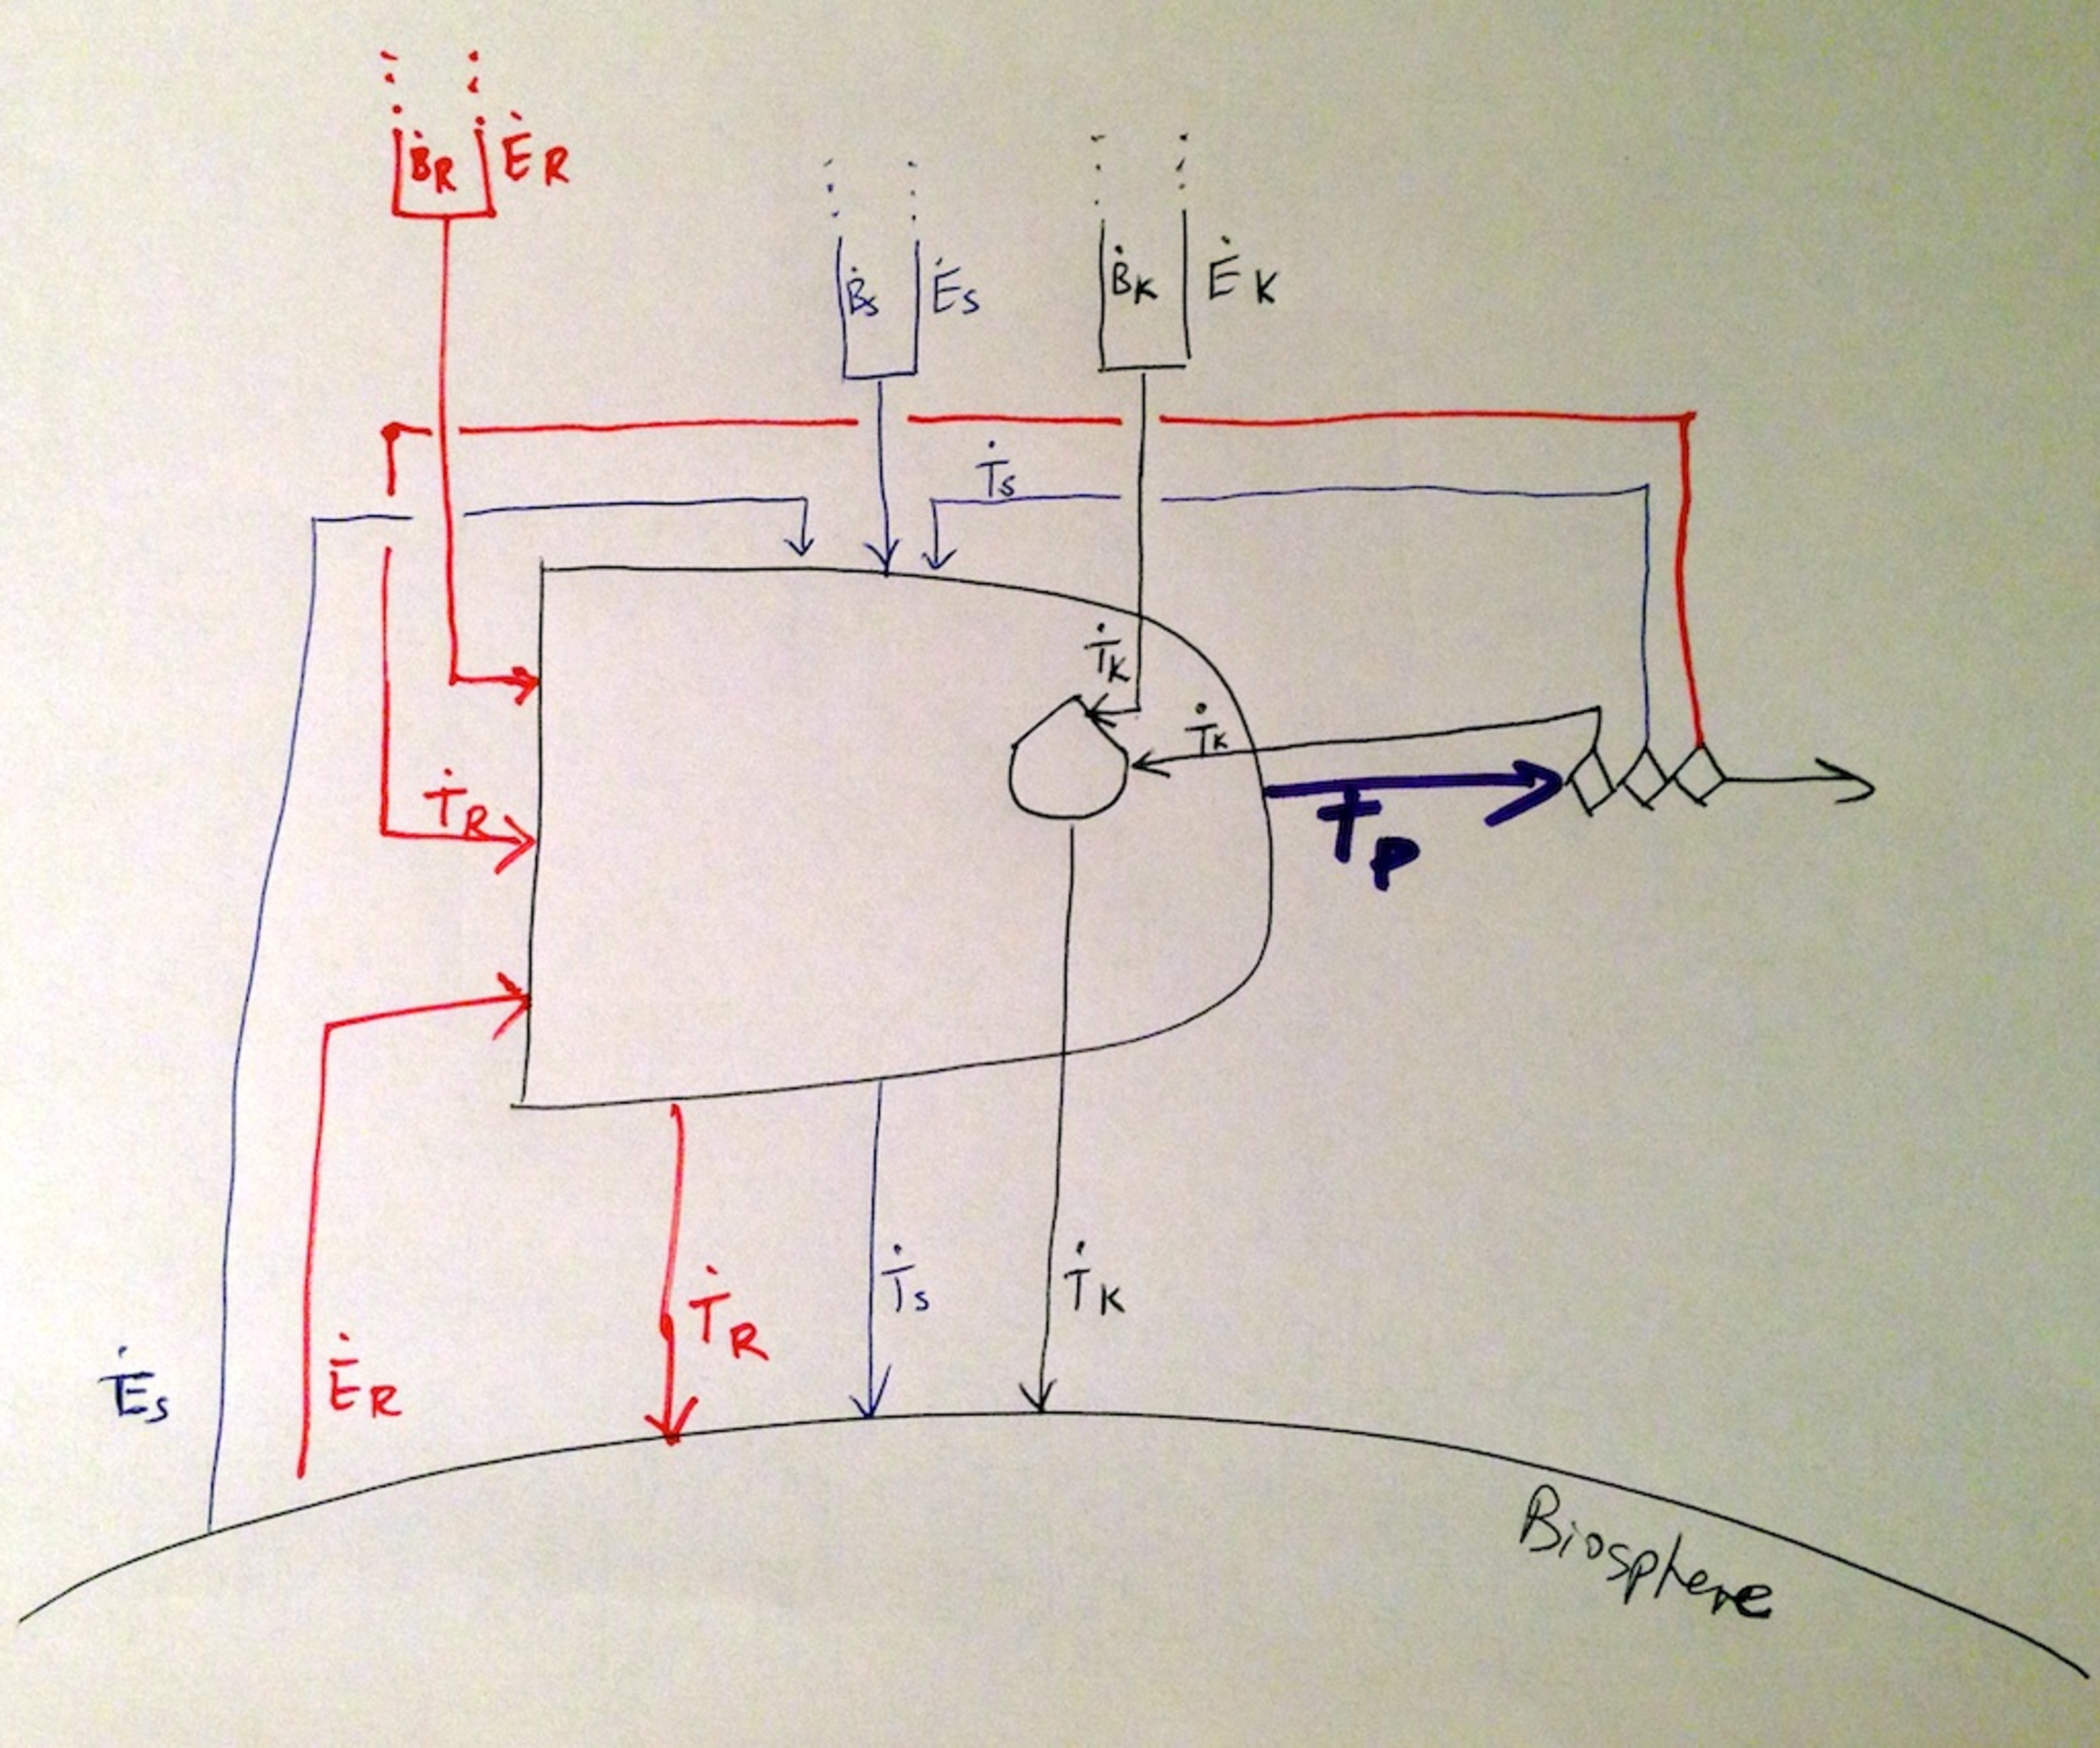
\includegraphics[width=.9\textwidth]{Part_2/Chapter_Embodied/images/TotalEnergyOneProducer.pdf}
	\caption{Total energy flows for a single sector of an economy. 
	For the sake of clarity, 
	embodied ($\dot{B}$) and direct ($\dot{E}$) energy
	are shown separately for material inflows from other sectors only.
	**** Mik: Can you make a figure that looks like this? 
	But, the waste streams should not be present. 
	I made a mistake to draw them. **** --Matt}
	\label{fig:embodied_single_producer}
\end{figure}

In some cases, a material flow may include 
either direct energy ($\dot{E}$) 
or embodied energy ($\dot{B}$), exclusive. 
For example, the flow of extracted crude oil from the earth 
consists of direct energy only ($\dot{B} = 0$ and $\dot{T} = \dot{E}$), 
because, in this method, no embodied energy ($B$) is added 
to the crude oil until it reaches the downstream side of the oil rig.
The material produced by a non-energy sector of the economy 
consists of indirect energy only ($\dot{E} \approx 0$, 
and therefore $\dot{T} \approx \dot{B}$), 
because direct energy ($E$) produced by 
a non-energy sector is negligible in this economy. 

In other cases, a material flow may include both direct energy flow
($\dot{E}$) \emph{and} embodied energy flow ($\dot{B}$) components.
For example, the outgoing flow of refined petroleum from the energy sector 
has both a direct energy ($\dot{E}$, the energy content of the oil product, 
usually represented by chemical potential energy) 
and embodied energy ($\dot{B}$, which accounts for the energy 
consumed in upstream processes 
to extract and refine the crude oil).\footnote{Outputs from 
agricultural sectors will be similar: 
both the direct energy component (comprising chemical potential energy) 
and the embodied energy component (representing upstream
energy consumed in food production) will be non-zero.}

Most of the I-O literature \cite{Bullard1975, Herendeen1978} 
[REF TO BULLARD AND HERENDEEN, ETC. HERE --MKH] assumes the following:

\begin{enumerate}
	\item flows of total energy ($\dot{T}$) are 
	\emph{conserved},\footnote{Total energy 
	can be neither created nor destroyed.}

	\item steady state conditions exist 
	(i.e., total energy does not accumulate in economic 
	sectors),\footnote{We will see later how the
	steady-state assumption in the literature 
	can introduce errors into I-O analyses.} and
	
	\item the sum of the signed 
	(input is positive, output is negative) 
	total energy inflows of a sector
	is assigned to the products of the sector (i.e., 
	there is no ``waste'' of total energy).
\end{enumerate}

Like the I-O literature, we assume that total energy is conserved
and never wasted.\footnote{Of course, waste heat exists and is
accounted by the First Law of Thermodynamics. However,
waste heat is ignored when accounting for total energy.}
However, we depart from the I-O literature to allow durability of goods 
as represented by total energy accumulation in economic sectors. 
Steady state, this approach is not. 

Total energy ($T$) may accumulate within an economic sector 
as stocks of direct energy materials 
(piles of coal or tanks of oil) 
but also as energy embodied in stocks of capital goods 
(e.g., machinery or buildings). 
The rate of accumulation of total energy 
in a sector of the economy, the biosphere, 
or society is given by the time derivative of total energy:

\begin{equation} \label{eq:T_accum_def}
	\frac{\mathrm{d}T}{\mathrm{d}t} 
	= \frac{\mathrm{d}E}{\mathrm{d}t} 
	+ \frac{\mathrm{d}B}{\mathrm{d}t}.
\end{equation}

The following equation provides a total energy accounting 
for a sector of the economy, where the $\dot{T}$ terms
are signed: positive for total energy input and negative
for total energy output.

\begin{equation} \label{eq:total_energy_accounting}
		\frac{\mathrm{d}T}{\mathrm{d}t}
		= \sum \dot{T}
\end{equation}

By substituting Equations~\ref{eq:T_dot_def} and
\ref{eq:T_accum_def} into 
Equation~\ref{eq:total_energy_accounting},
we obtain

\begin{equation} \label{eq:total_energy_accounting_details}
	\frac{\mathrm{d}E}{\mathrm{d}t} 
	+ \frac{\mathrm{d}B}{\mathrm{d}t}
	= \sum{\left( \dot{E} 
			+ \dot{B} \right)}.
\end{equation}


%+++++++++ Embodied Energy: Embodied Energy Accounting ++++++++++
\subsection{Embodied Energy Accounting}
%+++++++++

We note that the definition of total energy 
(Equation \ref{eq:T_def}) includes direct energy ($E$) 
and embodied energy ($B$) terms. 
On the other hand, the First Law of Thermodynamics 
(Equation~\ref{eq:First_Law_with_accumulation})
includes direct energy ($E$) and waste heat ($Q$) terms. 
The consequence of the foregoing difference is that 
an interesting relationship exists between embodied energy ($B$) 
and waste heat ($Q$). 

To derive an accounting equation for embodied energy, we substitute the 
First Law of Thermodynamics (Equation~\ref{eq:First_Law_with_accumulation})
into the total energy accounting equation (Equation~\ref{eq:total_energy_accounting_details}).

\begin{equation} \label{eq:embodied_energy_accounting}
	\frac{\mathrm{d}B}{\mathrm{d}t}
	= \sum \dot{B} 
	+ \sum \dot{Q}_{out}
\end{equation}

The waste energy terms ($\dot{Q}_{out}$) 
in Equation~\ref{eq:embodied_energy_accounting}
are \emph{outflows} of energy from the sector. 
The embodied energy 
terms ($\dot{B}$) represent embodied energy of either inflows
or outflows of material. Splitting the $\dot{B}$ term
into inflows and outflows gives

\begin{equation} \label{eq:embodied_energy_accounting_2}
	\frac{\mathrm{d}B}{\mathrm{d}t}
	= \sum \dot{B}_{in}
	- \sum \dot{B}_{out} 
	+ \sum \dot{Q}_{out}
\end{equation}

In words, the rate of accumulation of embodied energy 
in a sector of the economy 
$\left( \frac{\mathrm{d}B}{\mathrm{d}t} \right)$ 
is equal to the sum of the rates of 
inflow of embodied energy into the sector 
	($\sum \dot{B}_{in}$) 
less the rate of output of embodied energy from the sector 
	($\dot{B}_{out}$) 
\emph{plus} the rate of waste heat from the sector 
	($\dot{Q}_{out}$). 
The first two terms on the right side of
Equation~\ref{eq:embodied_energy_accounting_2} are expected: 
accumulation is the difference between inflow and outflow rates. 

Rearranging Equation~\ref{eq:embodied_energy_accounting_2}
yields another useful version of the equation.

\begin{equation} \label{eq:embodied_energy_accounting_3}
	\sum \dot{B}_{out}
	= \sum \dot{B}_{in}
	- \frac{\mathrm{d}B}{\mathrm{d}t} 
	+ \sum \dot{Q}_{out}
\end{equation}

We see that the waste energy term ($+\ \dot{Q}_{out}$) 
is \emph{additive} to both accumulation 
of embodied energy in a sector of the economy
(Equation \ref{eq:embodied_energy_accounting_2}) and 
outflow of embodied energy from a sector of the economy 
(Equation \ref{eq:embodied_energy_accounting_3}). 
Furthermore, because the waste direct energy 
($\dot{Q}_{out}$) appears 
in the embodied energy output from a sector, 
waste heat accumulates along each step of a process 
such that the energy embodied in a product 
is the \emph{sum} of waste heats along 
its upstream process path.

Equations~\ref{eq:embodied_energy_accounting_2}
and \ref{eq:embodied_energy_accounting_3} are generalized
embodied energy accounting equations that we will
apply to Examples~A--C in the sections that follow.


%%%%%%%%%% Embodied Energy: Example A %%%%%%%%%%
\section{Example A: single-sector economy}
%%%%%%%%%%

Figure \ref{fig:A_total_energy} shows the flows of total energy ($\dot{T}$) through the single-sector economy.

\begin{figure}[h!]
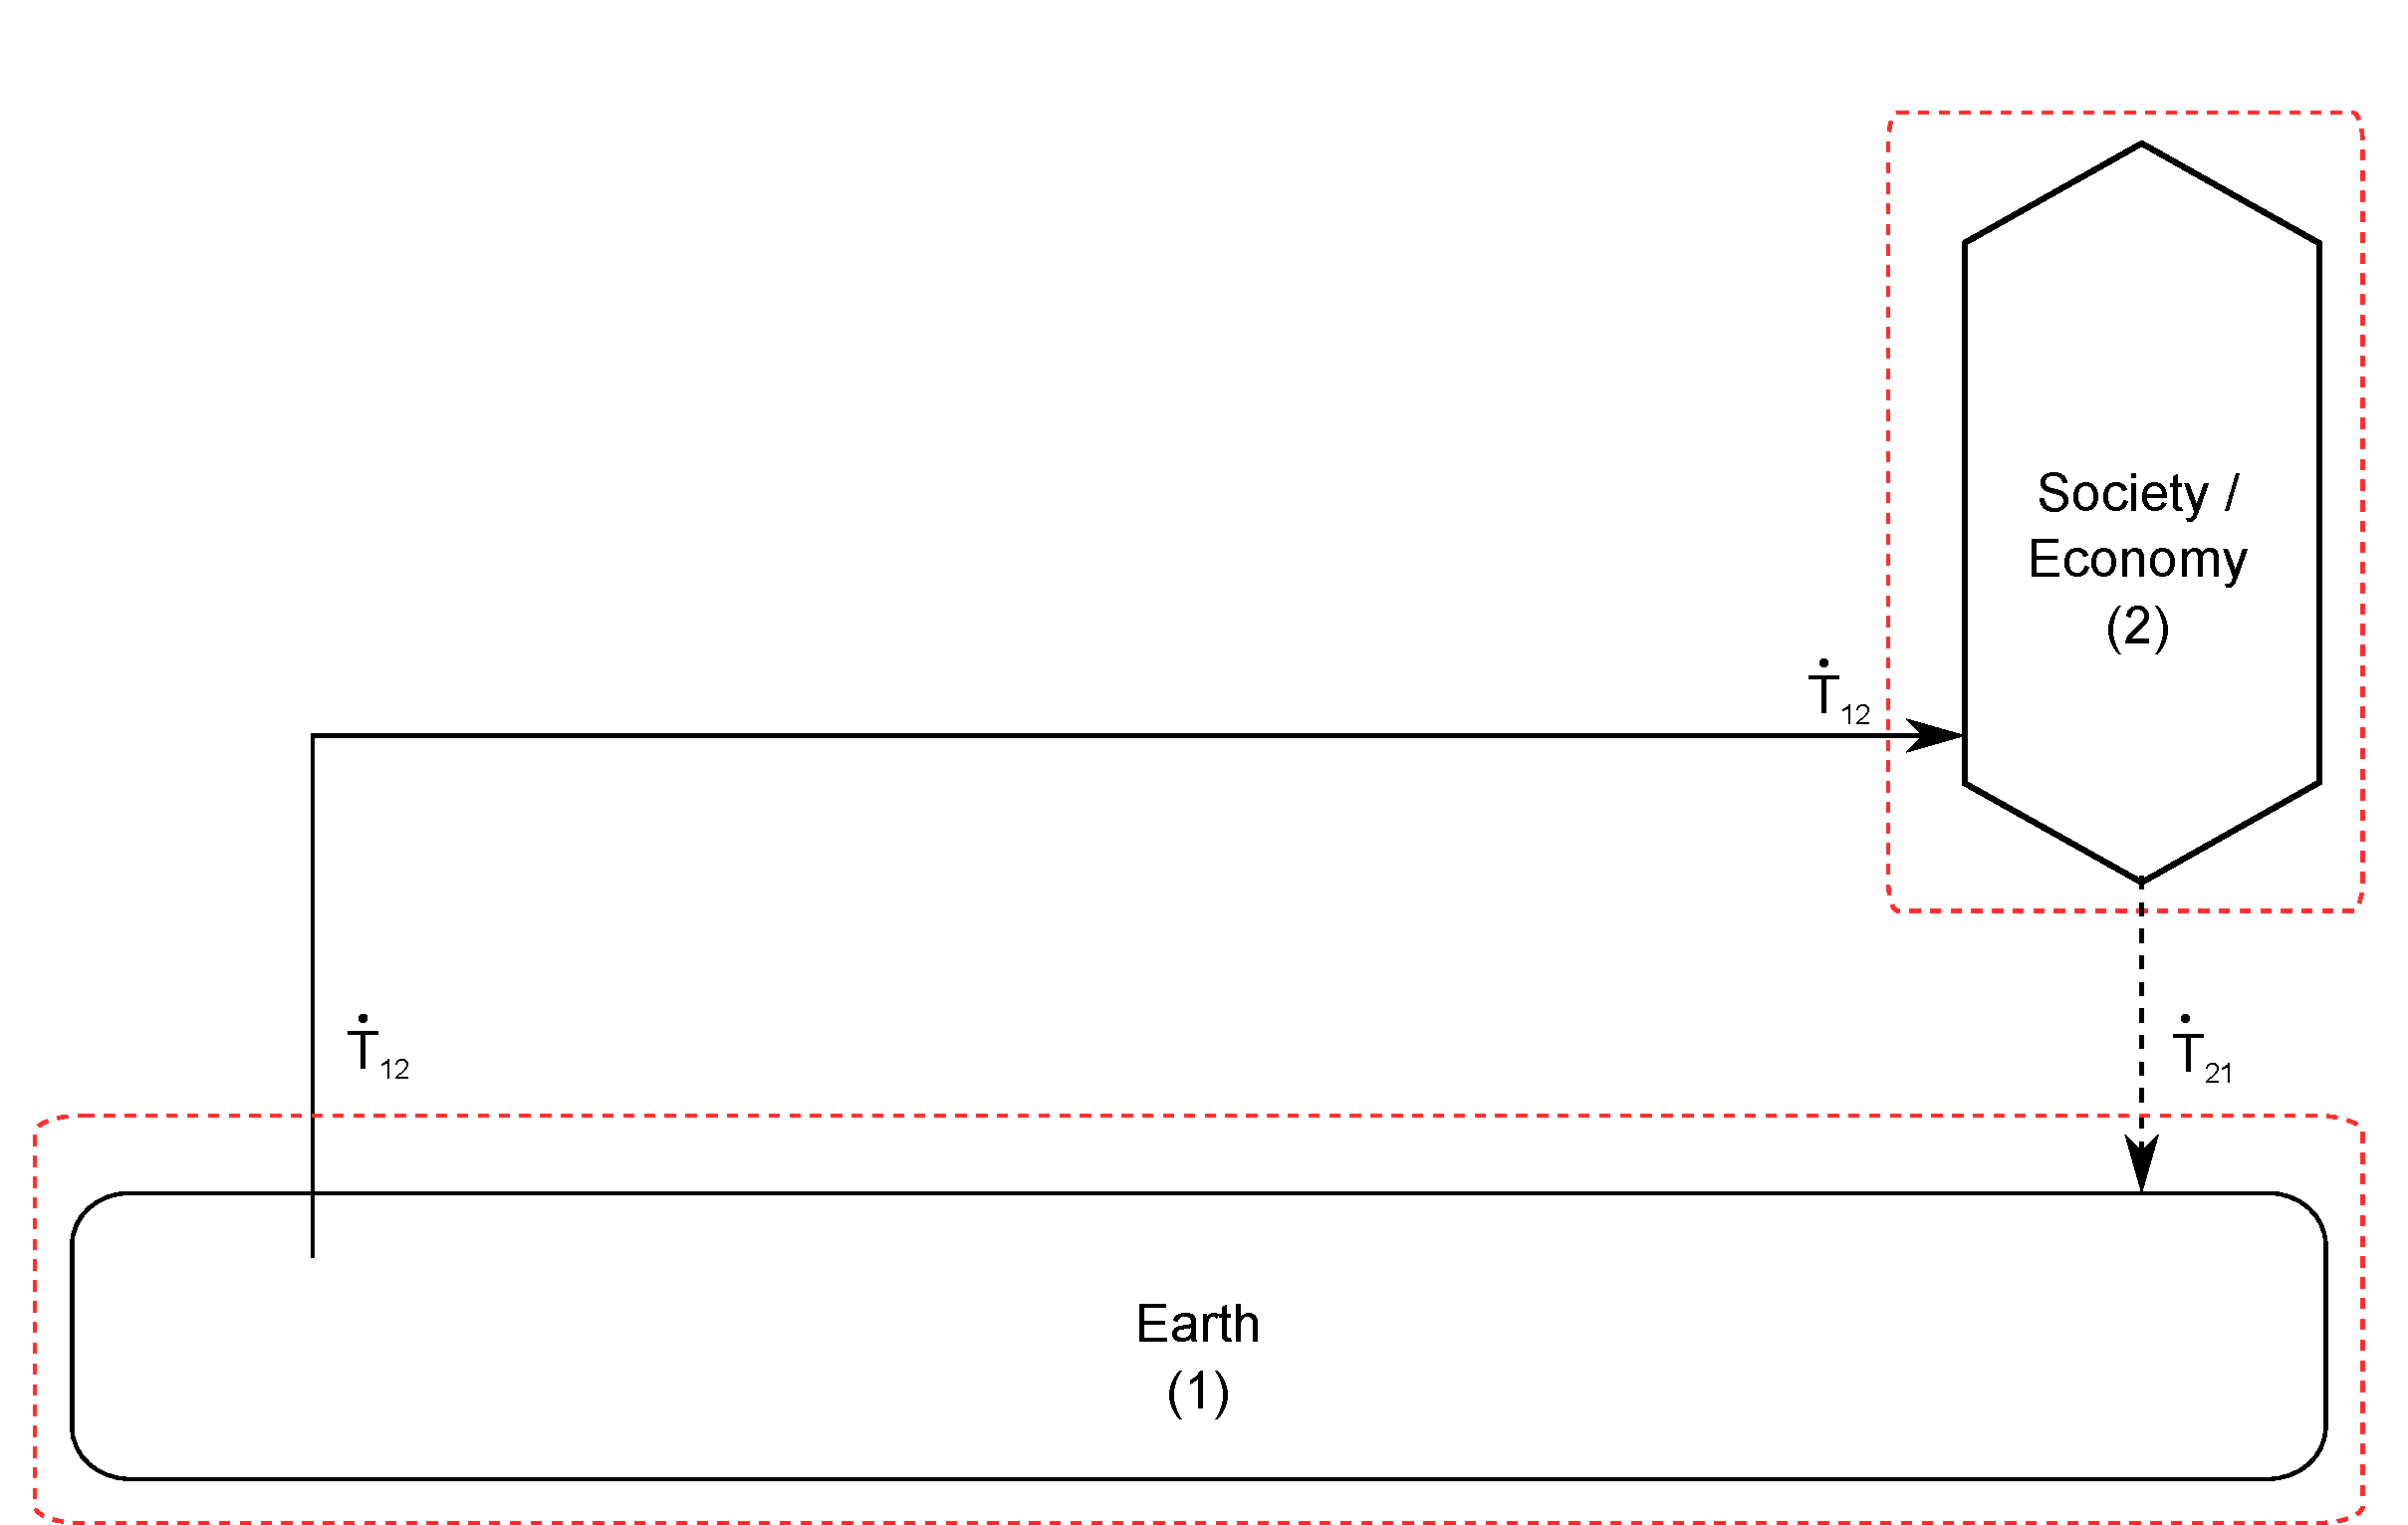
\includegraphics[width=1.0\linewidth]{Part_2/Chapter_Embodied/images/I-O_one_sector_total_energy.pdf}
\caption{Total energy flows ($\dot{T}$) in a single-sector Economy. 
**** Mik: Can you convert this figure to our new style? --Matt ****}
\label{fig:A_total_energy}
\end{figure}

As discussed above, we follow the I-O literature in assuming that 
total energy ($T$) is conserved. 
A total energy ($\dot{T}$) accounting around the 
single-sector economy (2) gives

\begin{equation} \label{eq:single_sector_T_with_accumulation}
	\frac{\mathrm{d}T_{2}}{\mathrm{d}t} 
	= \dot{T}_{12} 
	- \dot{T}_{21}.
\end{equation}

Substituting Equations~\ref{eq:T_dot_def} and
\ref{eq:T_accum_def} into 
Equation~\ref{eq:single_sector_T_with_accumulation}
yields

\begin{equation} \label{eq:A_total_energy}
	\frac{\mathrm{d}E_{2}}{\mathrm{d}t} 
	+ \frac{\mathrm{d}B_{2}}{\mathrm{d}t} 
	= \dot{E}_{12} 
	+ \dot{B}_{12} 
	- \dot{E}_{21}
	- \dot{B}_{21}.	
\end{equation}

Substituting the First Law of Thermodynamics 
(Equation~\ref{eq:dE_2/dt_single_sector}) 
into Equation~\ref{eq:A_total_energy} yields

\begin{equation} \label{eq:A_embodied_energy}
	\frac{\mathrm{d}B_{2}}{\mathrm{d}t} 
	= \dot{B}_{12} 
	- \dot{B}_{21}
	+ \dot{Q}_{21}.
\end{equation}

By definition, no embodied energy flows from 
the earth with extracted material, so we can 
simplify Equation~\ref{eq:A_embodied_energy}
as

\begin{equation} \label{eq:A_embodied_energy_2}
	\frac{\mathrm{d}B_{2}}{\mathrm{d}t} 
	= \dot{Q}_{21} 
	- \dot{B}_{21}.
\end{equation}

We turn now to Example B, a two-sector economy.


%%%%%%%%%% Embodied Energy: Example B %%%%%%%%%%
\section{Example B: two-sector economy}
%%%%%%%%%%

For the two-sector economy of Figures~\ref{fig:B_materials}
and \ref{fig:B_energy}, we again follow the I-O literature 
by assuming that total energy ($T$) is conserved. 
Figure~\ref{fig:B_total_energy} shows total energy
flows for the two-sector economy.

\begin{figure}[h!]
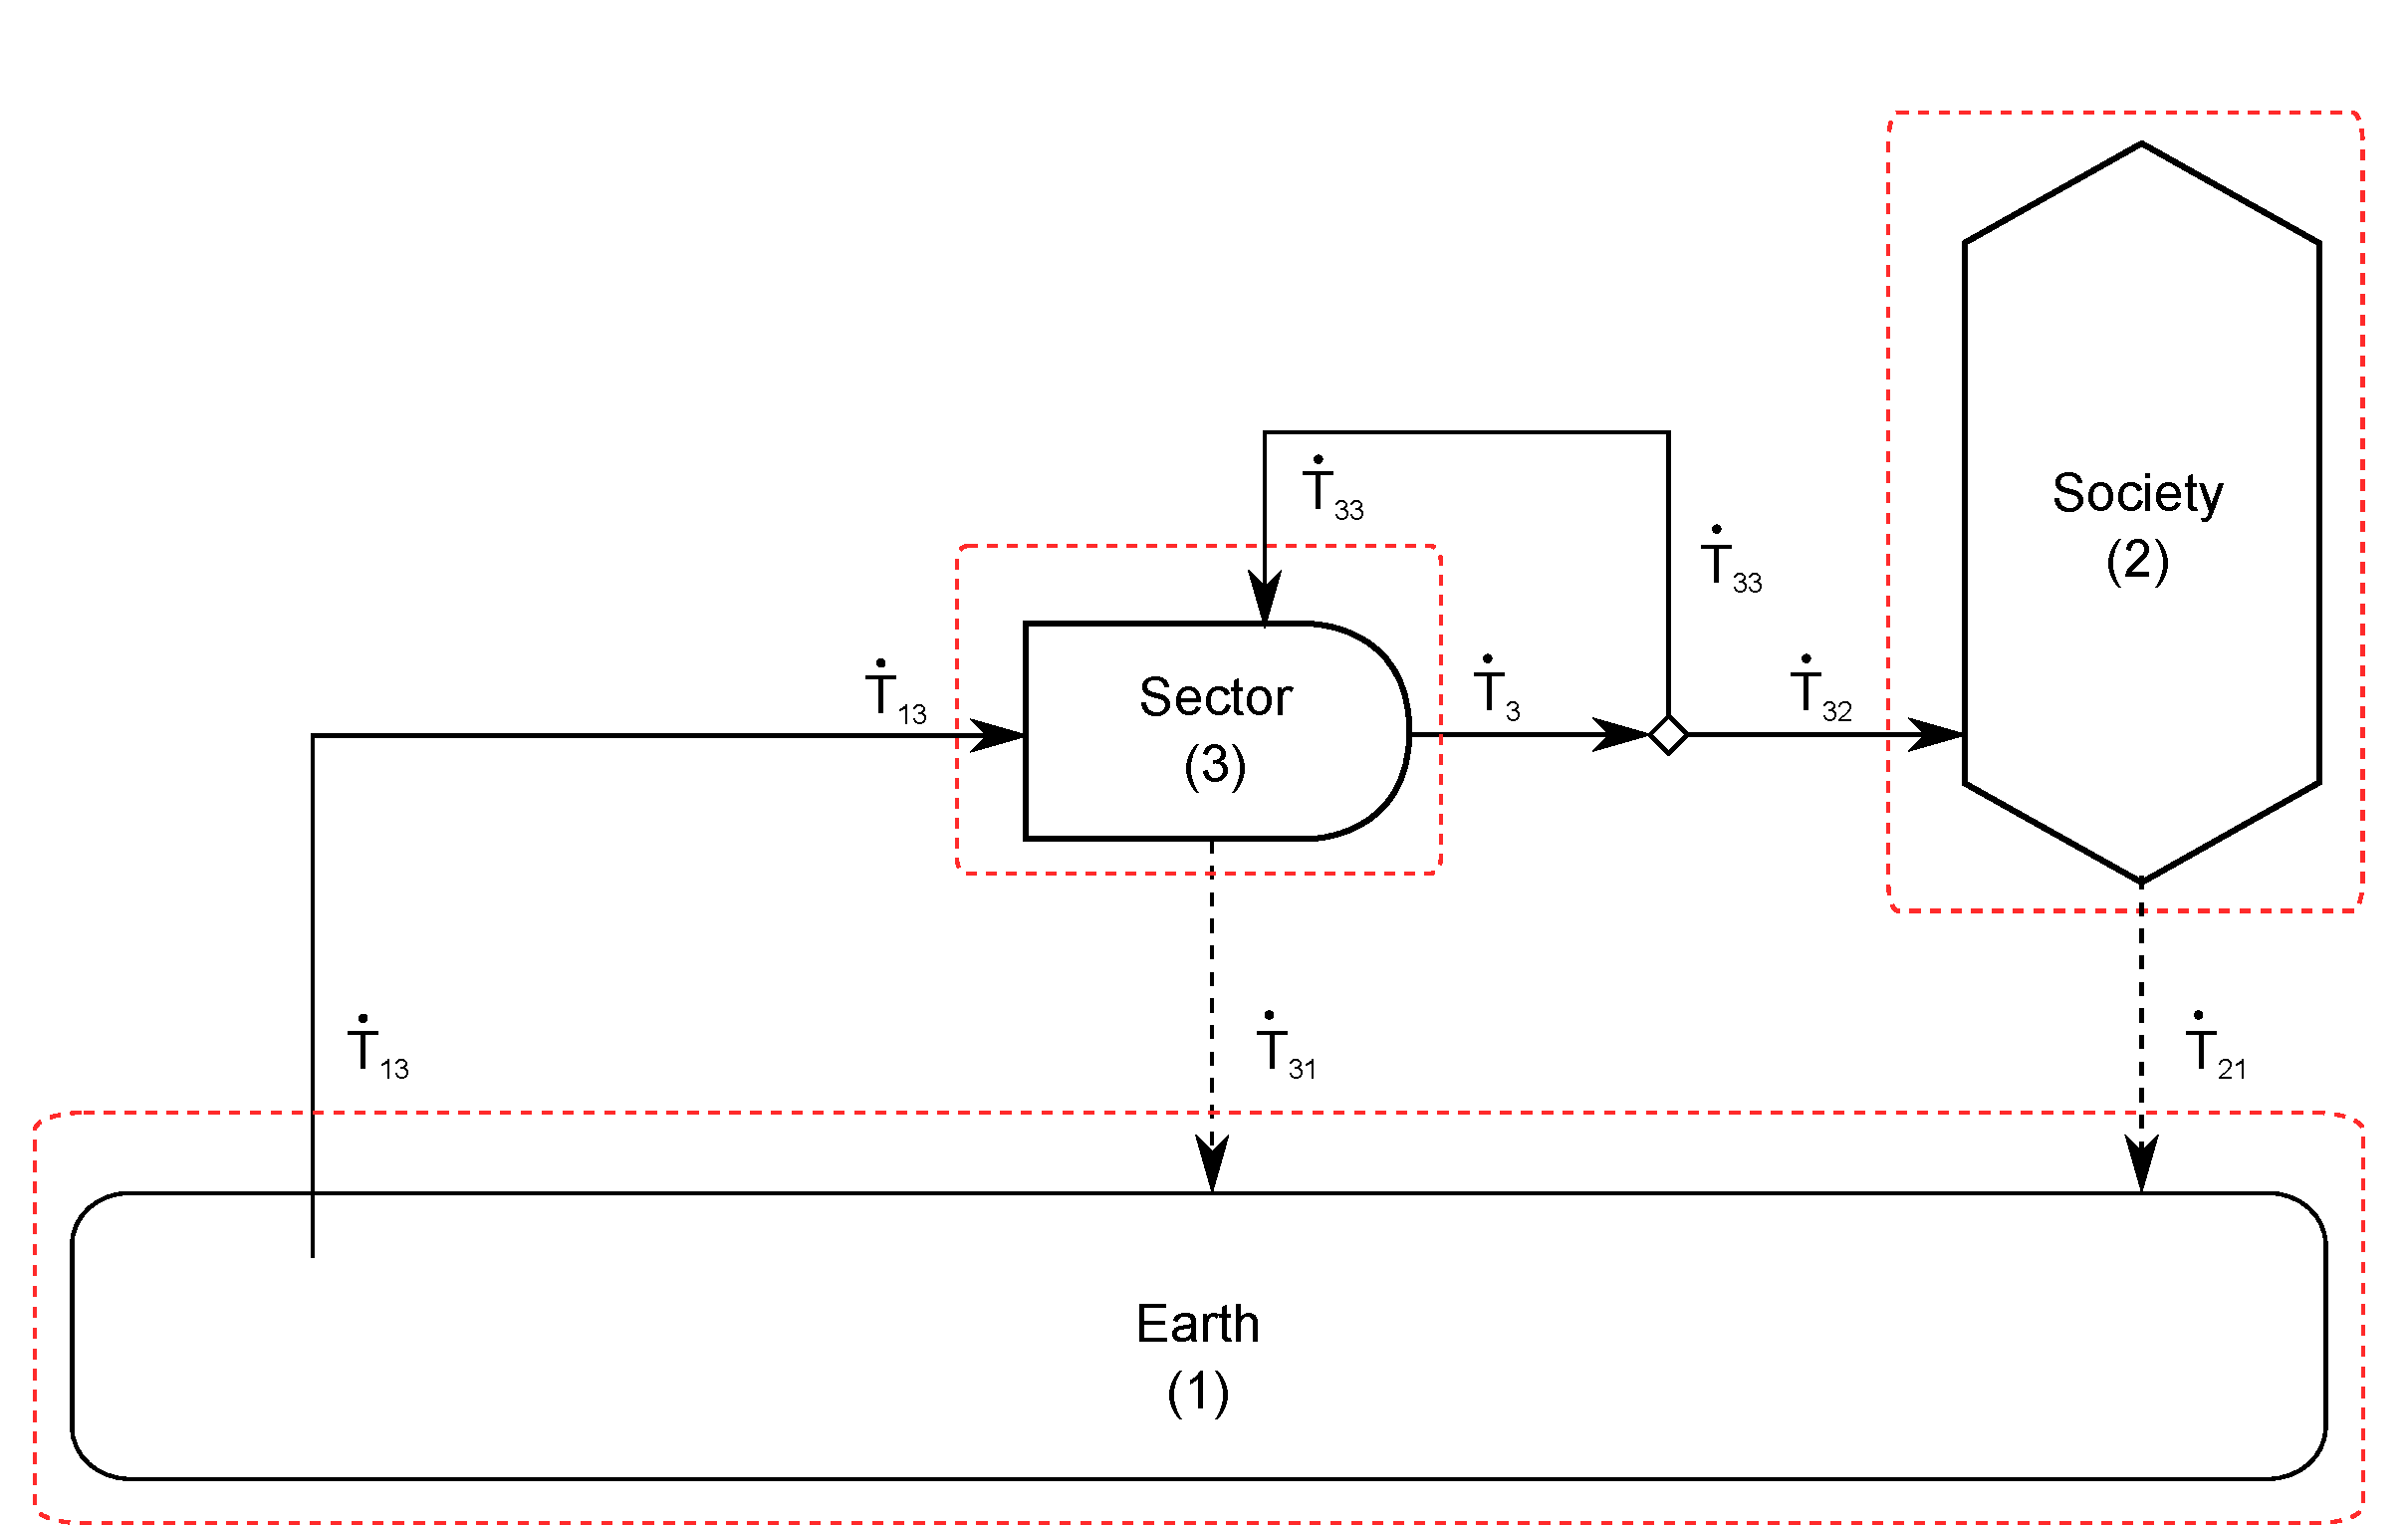
\includegraphics[width=0.9\linewidth]{Part_2/Chapter_Embodied/images/I-O_two_sector_total_energy.pdf}
\caption{Flows of total energy ($\dot{T}$) in a two-sector economy.
**** Mik: can you update this figure to our new style? --Matt ****}
\label{fig:B_total_energy}
\end{figure}

Accounting for accumulation of total energy and using the assumption 
that total energy is conserved, we can write the following equations.

\begin{equation} \label{eq:CV_T_1}
	\frac{\mathrm{d}T_{1}}{\mathrm{d}t} 	 
	= \dot{T}_{21} 
	+ \dot{T}_{31} 
	- \dot{T}_{13},
\end{equation}

\begin{equation} \label{eq:CV_T_2}
	\frac{\mathrm{d}T_{2}}{\mathrm{d}t} 	 
	= \dot{T}_{32} 
	- \dot{T}_{21},
\end{equation}

\noindent and

\begin{equation} \label{eq:CV_T_3}
	\frac{\mathrm{d}T_{3}}{\mathrm{d}t} 	 
	= \dot{T}_{13} 
	+ \dot{T}_{33} 
	- \dot{T}_{3} 
	- \dot{T}_{31}.
\end{equation}

**** Remove this assumption --Matt **** 
Given that 
$\frac{\mathrm{d}E_{i}}{\mathrm{d}t} 
		= 0$ and $\dot{T} = \dot{E} + \dot{B}$, 
we note that

\begin{equation} \label{eq:T_dot_equals_B_dot}
	\frac{\mathrm{d}T_i}{\mathrm{d}t} = \frac{\mathrm{d}B_i}{\mathrm{d}t},
\end{equation}

\noindent and we can rewrite 
the total energy accumulation accounting equations as

\begin{equation} \label{eq:CV_dB_1}
	\frac{\mathrm{d}B_{1}}{\mathrm{d}t} 
	= \dot{E}_{21} 
	+ \dot{B}_{21} 
	+ \dot{E}_{31} 
	+ \dot{B}_{31} 
	- \dot{E}_{13} 
	+ \dot{B}_{13},
\end{equation}

\begin{equation} \label{eq:CV_dB_2}
	\frac{\mathrm{d}B_{2}}{\mathrm{d}t} 
	= \dot{E}_{32} 
	+ \dot{B}_{32} 
	- \dot{E}_{21} 
	- \dot{B}_{21},
\end{equation}

\noindent and 

\begin{equation} \label{eq:CV_dB_3}
	\frac{\mathrm{d}B_{3}}{\mathrm{d}t} 
	= \dot{E}_{13} 
	+ \dot{B}_{13} 
	+ \dot{E}_{33} 
	+ \dot{B}_{33} 
	- \dot{E}_{3} 
	- \dot{B}_{3} 
	- \dot{E}_{31} 
	- \dot{B}_{31}.
\end{equation}

As in Example A, we can substitute the First Law of Thermodynamics 
for the economic Sector (Equation~\ref{eq:CV_E_dot_3_SS}) 
into the total energy accounting equation for the economic Sector 
(Equation~\ref{eq:CV_dB_3}). 
Assuming that $\dot{E}_{31} = 0$ 
(because energy is returned to the biosphere as waste heat, 
not direct energy), we obtain

\begin{equation} \label{eq:ExB_embodied_energy_accounting}
	\frac{\mathrm{d}B_3}{\mathrm{d}t} 
	= \dot{Q}_{31} 
	+ \dot{B}_{13} 
	+ \dot{B}_{33} 
	- \dot{B}_{31}
\end{equation}

Similar to Example~A, we observe that the accumulation rate 
of embodied energy in the Goods and Services sector (3) 
is the sum of the rates of waste heat from the sector 
($\dot{Q}_{31}$) and embodied energy into the sector 
($\dot{B}_{13} + \dot{B}_{33}$) 
less the rate of embodied energy leaving the sector 
on its output stream ($\dot{B}_{31}$).

In the next section, we apply embodied energy accounting to 
Example~C, a three-sector economy.


%%%%%%%%%% Embodied Energy: Example C %%%%%%%%%%
\section{Example C: three-sector economy}
%%%%%%%%%%

Again, we begin with a diagram showing total energy ($\dot{T}$) flows
among the economic sectors of Example~C.

\begin{figure}[h!]
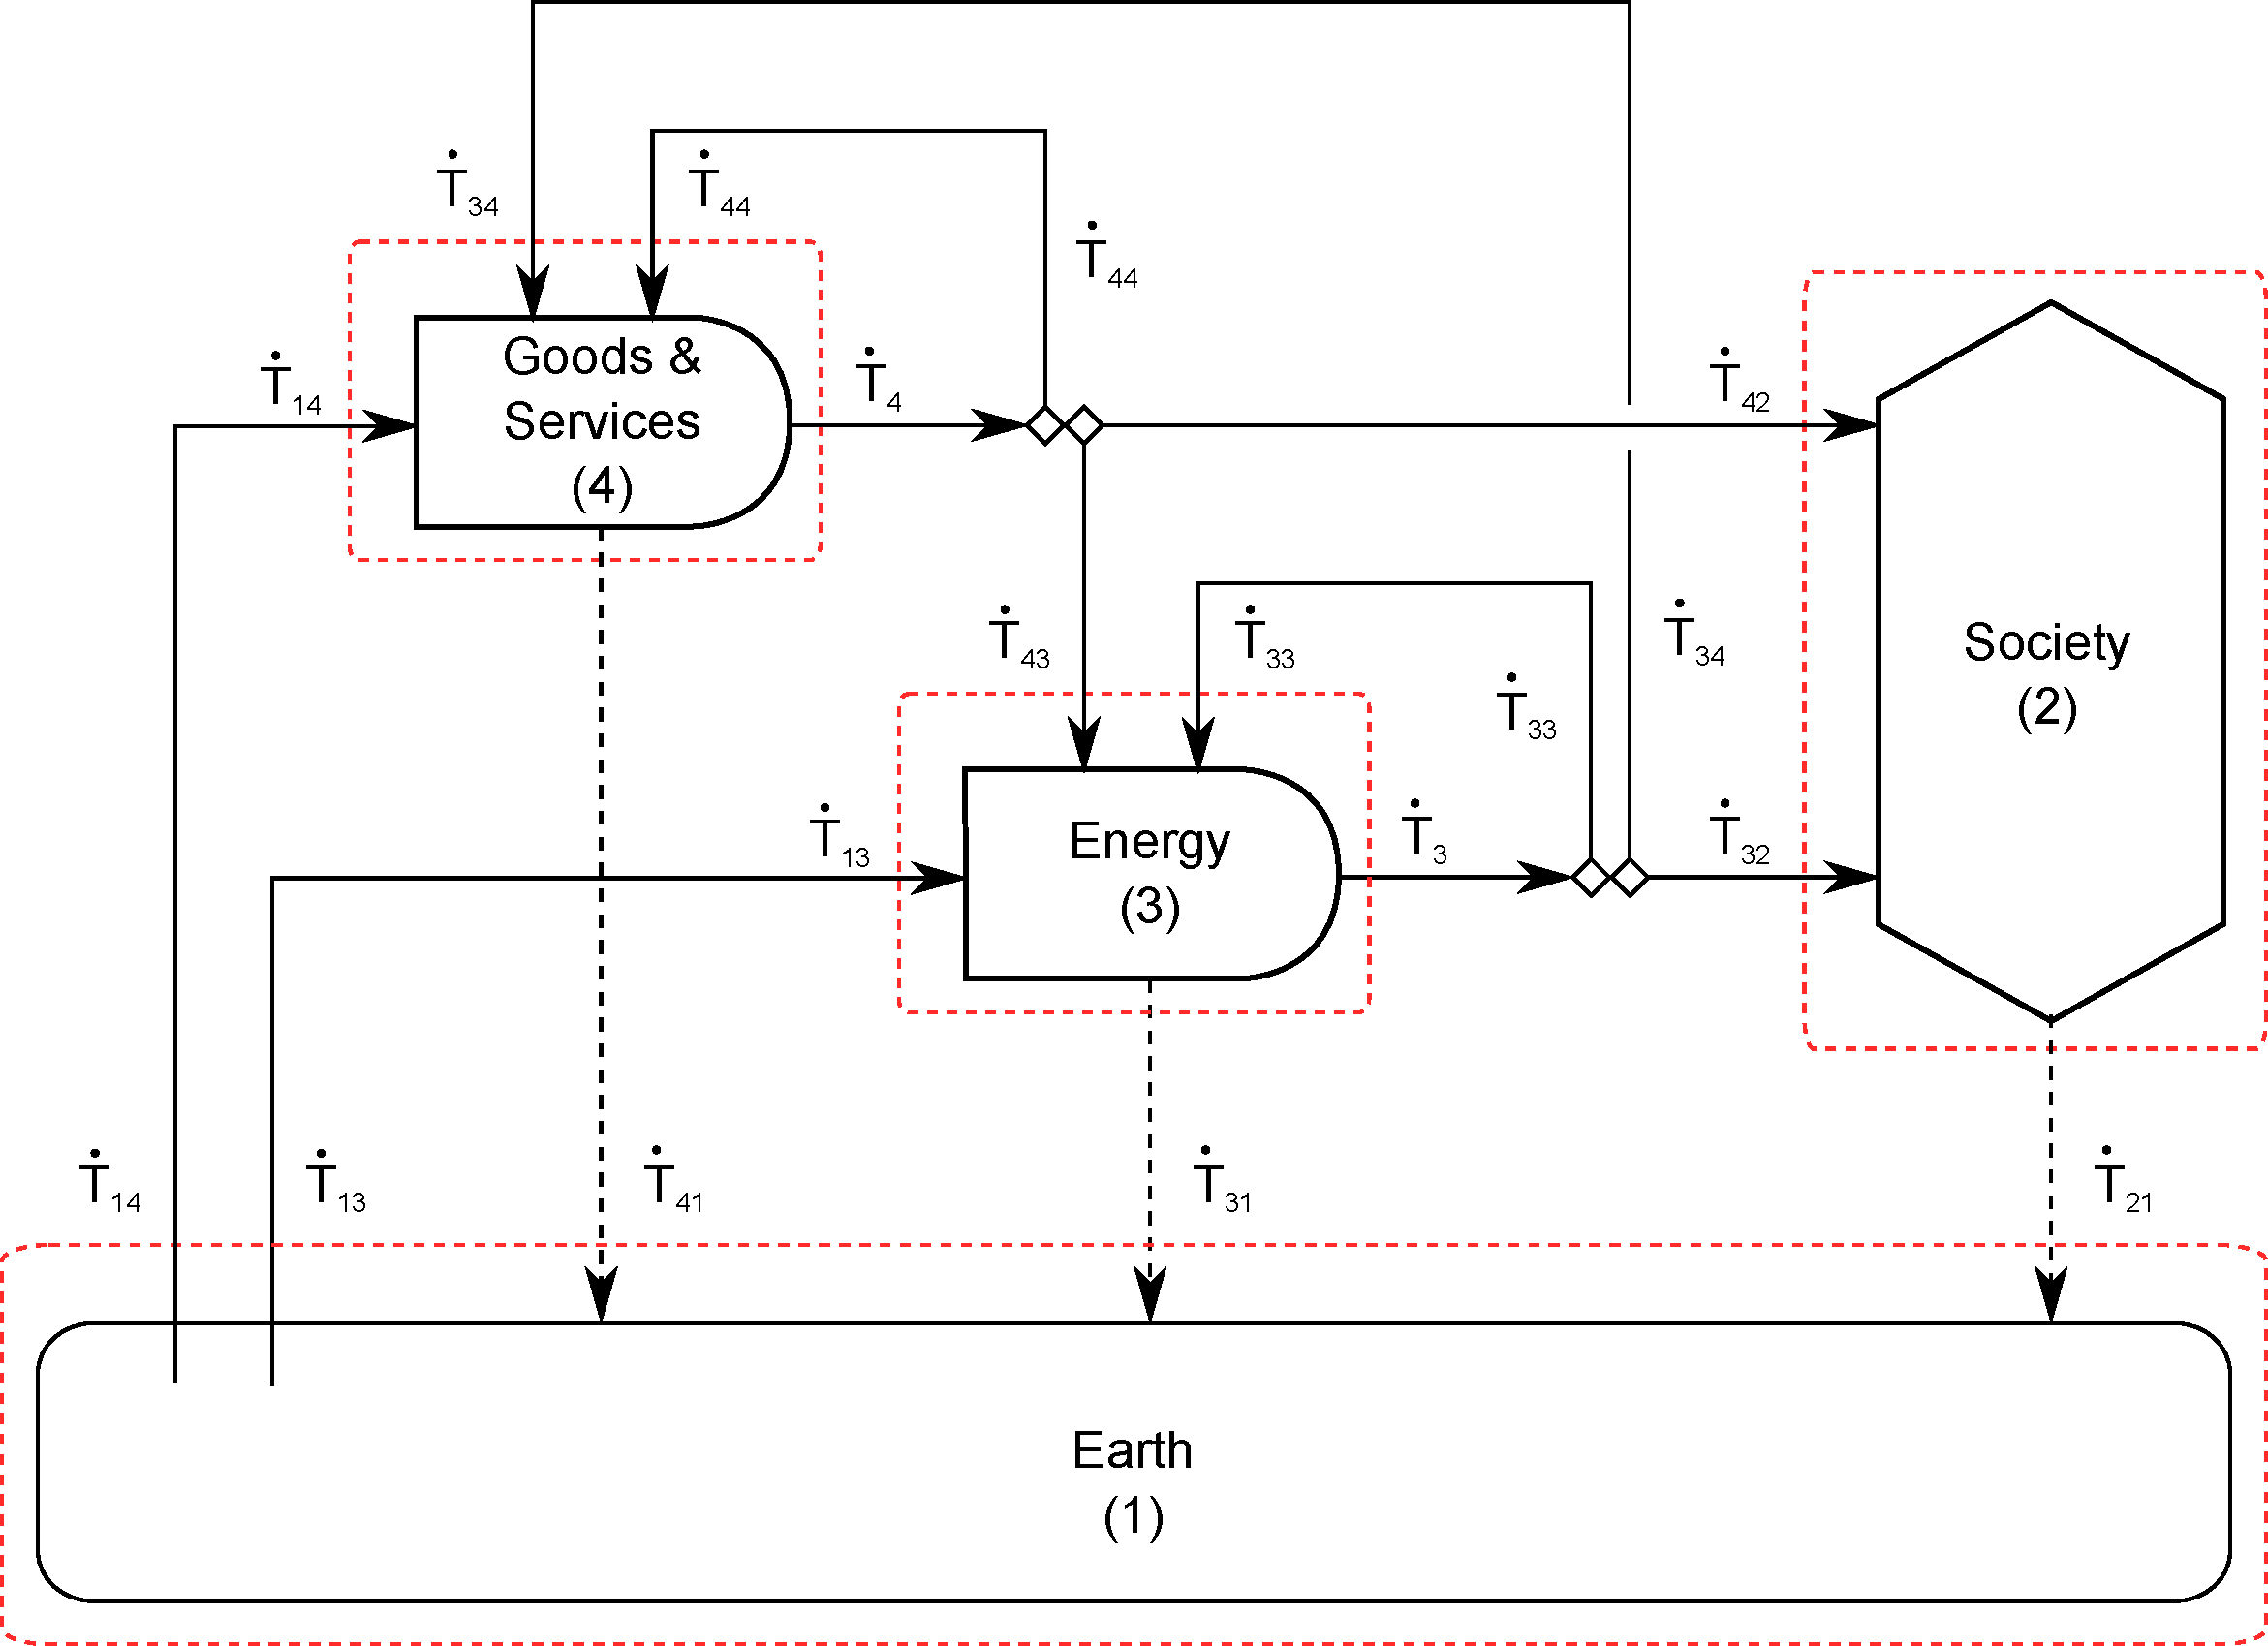
\includegraphics[width=1.0\linewidth]{Part_2/Chapter_Embodied/images/I-O_three_sector_total_energy.pdf}
\caption{Flows of total energy ($\dot{T}$) in a three-sector economy.
**** Mik: Can you update this figure to our new style? --Matt ****}
\label{fig:C_total_energy}
\end{figure}

Accounting for accumulation of total energy and 
applyingthe assumption that total energy is conserved, 
we can write the following equations.

\begin{equation} \label{eq:C-CV_T_1}
	\frac{\mathrm{d}T_{1}}{\mathrm{d}t} 	 
	= \dot{T}_{21} 
	+ \dot{T}_{31} 
	+ \dot{T}_{41} 
	- \dot{T}_{13} 
	- \dot{T}_{14},
\end{equation}

\begin{equation} \label{eq:C-CV_T_2}
	\frac{\mathrm{d}T_{2}}{\mathrm{d}t} 	 
	= \dot{T}_{32} 
	+ \dot{T}_{42} 
	- \dot{T}_{21},
\end{equation}

\begin{equation} \label{eq:C-CV_T_3}
	\frac{\mathrm{d}T_{3}}{\mathrm{d}t} 	 
	= \dot{T}_{13} 
	+ \dot{T}_{33} 
	+ \dot{T}_{43} 
	- \dot{T}_{3} 
	- \dot{T}_{31},
\end{equation}

\noindent and 

\begin{equation} \label{eq:C-CV_T_4}
	\frac{\mathrm{d}T_{4}}{\mathrm{d}t} 	 
	= \dot{T}_{14} 
	+ \dot{T}_{34} 
	+ \dot{T}_{44} 
	- \dot{T}_{4} 
	- \dot{T}_{41}.
\end{equation}

Substituting Equations~\ref{eq:T_dot_def} 
and \ref{eq:T_accum_def} into 
Equations~\ref{eq:C-CV_T_1} through
\ref{eq:C-CV_T_4} gives

\begin{equation} \label{eq:C-CV_dB_1}
	\frac{\mathrm{d}E_{1}}{\mathrm{d}t}
	+ \frac{\mathrm{d}B_{1}}{\mathrm{d}t}
	= \dot{E}_{21} 
	+ \dot{B}_{21} 
	+ \dot{E}_{31} 
	+ \dot{B}_{31} 
	+ \dot{E}_{41} 
	+ \dot{B}_{41} 
	- \dot{E}_{13} 
	- \dot{B}_{13} 
	- \dot{E}_{14} 
	- \dot{B}_{14},
\end{equation}

\begin{equation} \label{eq:C-CV_dB_2}
	\frac{\mathrm{d}E_{2}}{\mathrm{d}t} 
	+ \frac{\mathrm{d}B_{2}}{\mathrm{d}t} 	 
	= \dot{E}_{32} 
	+ \dot{B}_{32} 
	+ \dot{E}_{42} 
	+ \dot{B}_{42} 
	- \dot{E}_{21} 
	- \dot{B}_{21},
\end{equation}

\begin{equation} \label{eq:C-CV_dB_3}
	\frac{\mathrm{d}E_{3}}{\mathrm{d}t} 
	+ \frac{\mathrm{d}B_{3}}{\mathrm{d}t} 	 
	= \dot{E}_{13} 
	+ \dot{B}_{13} 
	+ \dot{E}_{33} 
	+ \dot{B}_{33} 
	+ \dot{E}_{43} 
	+ \dot{B}_{43} 
	- \dot{E}_{3} 
	- \dot{B}_{3} 
	- \dot{E}_{31} 
	- \dot{B}_{31},
\end{equation}

\noindent and 

\begin{equation} \label{eq:C-CV_dB_4}
	\frac{\mathrm{d}E_{4}}{\mathrm{d}t} 
	+ \frac{\mathrm{d}B_{4}}{\mathrm{d}t} 	 
	= \dot{E}_{14} 
	+ \dot{B}_{14} 
	+ \dot{E}_{34} 
	+ \dot{B}_{34}
	+ \dot{E}_{44} 
	+ \dot{B}_{44} 
	- \dot{E}_{4} 
	- \dot{B}_{4} 
	- \dot{E}_{41} 
	- \dot{B}_{41}.
\end{equation}

Substituting the First Law of Thermodynamics 
(Equations~\ref{eq:C-CV_E_dot_4_simp} through \ref{eq:C-CV_E_dot_3}) 
into the total energy accounting equations 
(Equations \ref{eq:C-CV_dB_1} through \ref{eq:C-CV_dB_4}) 
gives embodied energy accounting equations for Example~C.

\begin{equation} \label{eq:C-embodied_acct_1}
	\frac{\mathrm{d}B_{1}}{\mathrm{d}t} 	 
	= \dot{B}_{21} 
	+ \dot{B}_{31} 
	+ \dot{B}_{41} 
	- \dot{B}_{13} 
	- \dot{B}_{14} 
	- \dot{Q}_{21} 
	- \dot{Q}_{31} 
	- \dot{Q}_{41}
\end{equation}

\begin{equation} \label{eq:C-embodied_acct_2}
	\frac{\mathrm{d}B_{2}}{\mathrm{d}t} 	 
	= \dot{B}_{32} 
	+ \dot{B}_{42} 
	+ \dot{Q}_{21} 
	- \dot{B}_{21}
\end{equation}

\begin{equation} \label{eq:C-embodied_acct_3}
	\frac{\mathrm{d}B_{3}}{\mathrm{d}t} 	 
	= \dot{B}_{13} 
	+ \dot{B}_{33} 
	+ \dot{B}_{43} 
	+ \dot{Q}_{31} 
	- \dot{B}_{3} 
	- \dot{B}_{31}
\end{equation}

\begin{equation} \label{eq:C-embodied_acct_4}
	\frac{\mathrm{d}B_{4}}{\mathrm{d}t}	 
	= \dot{B}_{14} 
	+ \dot{B}_{34} 
	+ \dot{B}_{44} 
	+ \dot{Q}_{41} 
	- \dot{B}_{4} 
	- \dot{B}_{41}
\end{equation}

To verify the above derivation, 
we sum Equations~\ref{eq:C-embodied_acct_1} through 
\ref{eq:C-embodied_acct_4} 
and use the following identities:

\begin{equation} \label{eq:C-B_sum_3_output}
	\dot{B}_3 
	= \dot{B}_{32} 
	+ \dot{B}_{33} 
	+ \dot{B}_{34}
\end{equation}

\noindent and

\begin{equation} \label{eq:C-B_sum_4_output}
	\dot{B}_4 
	= \dot{B}_{42} 
	+ \dot{B}_{43} 
	+ \dot{B}_{44};
\end{equation}

\noindent to obtain

\begin{equation} \label{eq:C-B_sums_to_zero}
	\frac{\mathrm{d}B_{1}}{\mathrm{d}t} 
	+ \frac{\mathrm{d}B_{2}}{\mathrm{d}t} 
	+ \frac{\mathrm{d}B_{3}}{\mathrm{d}t} 
	+ \frac{\mathrm{d}B_{4}}{\mathrm{d}t} 
	= 0,
\end{equation}

\noindent as expected. The total embodied energy content of the system 
(biosphere (1), society (2), energy sector (3), and goods and services sector (4)) 
remains constant with respect to time.



\bibliography{../../EROI_review_v2}
\bibliographystyle{unsrt}


% Always give a unique label
% and use \ref{<label>} for cross-references
% and \cite{<label>} for bibliographic references
% use \sectionmark{}
% to alter or adjust the section heading in the running head
%% Instead of simply listing headings of different levels we recommend to let every heading be followed by at least a short passage of text. Furtheron please use the \LaTeX\ automatism for all your cross-references and citations.

%% Please note that the first line of text that follows a heading is not indented, whereas the first lines of all sequent paragraphs are.

%% Use the standard \verb|equation| environment to typeset your equations, e.g.
%
%% \begin{equation}
%% a \times b = c\;,
%% \end{equation}
%
%% however, for multiline equations we recommend to use the \verb|eqnarray|
%% environment\footnote{In physics texts please activate the class option \texttt{vecphys} to depict your vectors in \textbf{\itshape boldface-italic} type - as is customary for a wide range of physical jects.}.
%% \begin{eqnarray}
%% a \times b = c \nonumber\\
%% \vec{a} \cdot \vec{b}=\vec{c}
%% \label{eq:01}
%% \end{eqnarray}

%% \section{section Heading}
%% \label{sec:2}
%% Instead of simply listing headings of different levels we recommend to let every heading be followed by at least a short passage of text. Furtheron please use the \LaTeX\ automatism for all your cross-references\index{cross-references} and citations\index{citations} as has already been described in Sect.~\ref{sec:2}.

%% \begin{quotation}
%% Please do not use quotation marks when quoting texts! Simply use the \verb|quotation| environment -- it will automatically render Springer's preferred layout.
%% \end{quotation}


%% \section{section Heading}
%% Instead of simply listing headings of different levels we recommend to let every heading be followed by at least a short passage of text. Furtheron please use the \LaTeX\ automatism for all your cross-references and citations as has already been described in Sect.~\ref{sec:2}, see also Fig.~\ref{fig:1}\footnote{If you copy text passages, figures, or tables from other works, you must obtain \textit{permission} from the copyright holder (usually the original publisher). Please enclose the signed permission with the manucript. The sources\index{permission to print} must be acknowledged either in the captions, as footnotes or in a separate section of the book.}

%% Please note that the first line of text that follows a heading is not indented, whereas the first lines of all sequent paragraphs are.

% For figures use
%
%% \begin{figure}[b]
%% \sidecaption
% Use the relevant command for your figure-insertion program
% to insert the figure file.
% For example, with the option graphics use
%% \includegraphics[scale=.65]{figure}
%
% If not, use
%\picplace{5cm}{2cm} % Give the correct figure height and width in cm
%
%% \caption{If the width of the figure is less than 7.8 cm use the \texttt{sidecapion} command to flush the caption on the left side of the page. If the figure is positioned at the top of the page, align the sidecaption with the top of the figure -- to achieve this you simply need to use the optional argument \texttt{[t]} with the \texttt{sidecaption} command}
%% \label{fig:1}       % Give a unique label
%% \end{figure}


%% \paragraph{Paragraph Heading} %
%% Instead of simply listing headings of different levels we recommend to let every heading be followed by at least a short passage of text. Furtheron please use the \LaTeX\ automatism for all your cross-references and citations as has already been described in Sect.~\ref{sec:2}.

%% Please note that the first line of text that follows a heading is not indented, whereas the first lines of all sequent paragraphs are.

%% For typesetting numbered lists we recommend to use the \verb|enumerate| environment -- it will automatically render Springer's preferred layout.

%% \begin{enumerate}
%% \item{Livelihood and survival mobility are oftentimes coutcomes of uneven socioeconomic development.}
%% \begin{enumerate}
%% \item{Livelihood and survival mobility are oftentimes coutcomes of uneven socioeconomic development.}
%% \item{Livelihood and survival mobility are oftentimes coutcomes of uneven socioeconomic development.}
%% \end{enumerate}
%% \item{Livelihood and survival mobility are oftentimes coutcomes of uneven socioeconomic development.}
%% \end{enumerate}


%% \paragraph{paragraph Heading} In order to avoid simply listing headings of different levels we recommend to let every heading be followed by at least a short passage of text. Use the \LaTeX\ automatism for all your cross-references and citations as has already been described in Sect.~\ref{sec:2}, see also Fig.~\ref{fig:2}.

%% Please note that the first line of text that follows a heading is not indented, whereas the first lines of all sequent paragraphs are.

%% For unnumbered list we recommend to use the \verb|itemize| environment -- it will automatically render Springer's preferred layout.

%% \begin{itemize}
%% \item{Livelihood and survival mobility are oftentimes coutcomes of uneven socioeconomic development, cf. Table~\ref{tab:1}.}
%% \begin{itemize}
%% \item{Livelihood and survival mobility are oftentimes coutcomes of uneven socioeconomic development.}
%% \item{Livelihood and survival mobility are oftentimes coutcomes of uneven socioeconomic development.}
%% \end{itemize}
%% \item{Livelihood and survival mobility are oftentimes coutcomes of uneven socioeconomic development.}
%% \end{itemize}

%% \begin{figure}[t]
%% \sidecaption[t]
% Use the relevant command for your figure-insertion program
% to insert the figure file.
% For example, with the option graphics use
%% \includegraphics[scale=.65]{figure}
%
% If not, use
%\picplace{5cm}{2cm} % Give the correct figure height and width in cm
%
%% \caption{Please write your figure caption here}
%% \label{fig:2}       % Give a unique label
%% \end{figure}

%% \runinhead{Run-in Heading Boldface Version} Use the \LaTeX\ automatism for all your cross-references and citations as has already been described in Sect.~\ref{sec:2}.

%% \runinhead{Run-in Heading Italic Version} Use the \LaTeX\ automatism for all your cross-refer\-ences and citations as has already been described in Sect.~\ref{sec:2}\index{paragraph}.
% Use the \index{} command to code your index words
%
% For tables use
%
%% \begin{table}
%% \caption{Please write your table caption here}
%% \label{tab:1}       % Give a unique label
%
% For LaTeX tables use
%
%% \begin{tabular}{p{2cm}p{2.4cm}p{2cm}p{4.9cm}}
%% \hline\noalign{\smallskip}
%% Classes & class & Length & Action Mechanism  \\
%% \noalign{\smallskip}\svhline\noalign{\smallskip}
%% Translation & mRNA$^a$  & 22 (19--25) & Translation repression, mRNA cleavage\\
%% Translation & mRNA cleavage & 21 & mRNA cleavage\\
%% Translation & mRNA  & 21--22 & mRNA cleavage\\
%%Translation & mRNA  & 24--26 & Histone and DNA Modification\\
%%\noalign{\smallskip}\hline\noalign{\smallskip}
%%\end{tabular}
%%$^a$ Table foot note (with superscript)
%%\end{table}
%
%% \section{Section Heading}
%%\label{sec:3}
% Always give a unique label
% and use \ref{<label>} for cross-references
% and \cite{<label>} for bibliographic references
% use \sectionmark{}
% to alter or adjust the section heading in the running head
%% Instead of simply listing headings of different levels we recommend to let every heading be followed by at least a short passage of text. Furtheron please use the \LaTeX\ automatism for all your cross-references and citations as has already been described in Sect.~\ref{sec:2}.

%% Please note that the first line of text that follows a heading is not indented, whereas the first lines of all sequent paragraphs are.

%%If you want to list definitions or the like we recommend to use the Springer-enhanced \verb|description| environment -- it will automatically render Springer's preferred layout.

%%\begin{description}[Type 1]
%%\item[Type 1]{That addresses central themes pertainng to migration, health, and disease. In Sect.~\ref{sec:1}, Wilson discusses the role of human migration in infectious disease distributions and patterns.}
%%\item[Type 2]{That addresses central themes pertainng to migration, health, and disease. In Sect.~\ref{sec:2}, Wilson discusses the role of human migration in infectious disease distributions and patterns.}
%%\end{description}

%%\section{section Heading} %
%% In order to avoid simply listing headings of different levels we recommend to let every heading be followed by at least a short passage of text. Use the \LaTeX\ automatism for all your cross-references and citations citations as has already been described in Sect.~\ref{sec:2}.

%% Please note that the first line of text that follows a heading is not indented, whereas the first lines of all sequent paragraphs are.

%% \begin{svgraybox}
%% If you want to emphasize complete paragraphs of texts we recommend to use the newly defined Springer class option \verb|graybox| and the newly defined environment \verb|svgraybox|. This will produce a 15 percent screened box 'behind' your text.

%% If you want to emphasize complete paragraphs of texts we recommend to use the newly defined Springer class option and environment \verb|svgraybox|. This will produce a 15 percent screened box 'behind' your text.
%% \end{svgraybox}


%% \section{section Heading}
%%Instead of simply listing headings of different levels we recommend to let every heading be followed by at least a short passage of text. Furtheron please use the \LaTeX\ automatism for all your cross-references and citations as has already been described in Sect.~\ref{sec:2}.

%% Please note that the first line of text that follows a heading is not indented, whereas the first lines of all sequent paragraphs are.

%% \begin{theorem}
%% Theorem text goes here.
%% \end{theorem}
%
% or
%
%% \begin{definition}
%% Definition text goes here.
%% \end{definition}

%% \begin{proof}
%\smartqed
%% Proof text goes here.
%% \qed
%% \end{proof}

%%\paragraph{Paragraph Heading} %
%% Instead of simply listing headings of different levels we recommend to let every heading be followed by at least a short passage of text. Furtheron please use the \LaTeX\ automatism for all your cross-references and citations as has already been described in Sect.~\ref{sec:2}.

%% Note that the first line of text that follows a heading is not indented, whereas the first lines of all subsequent paragraphs are.
%
% For built-in environments use
%
%%\begin{theorem}
%%Theorem text goes here.
%%\end{theorem}
%
%%\begin{definition}
%%Definition text goes here.
%%\end{definition}
%
%%\begin{proof}
%%\smartqed
%% Proof text goes here.
%%\qed
%%\end{proof}
%
%% \begin{acknowledgement}
%% If you want to include acknowledgments of assistance and the like at the end of an individual chapter please use the \verb|acknowledgement| environment -- it will automatically render Springer's preferred layout.
%% \end{acknowledgement}
%
%% \section*{Appendix}
%% \addcontentsline{toc}{section}{Appendix}
%
%% When placed at the end of a chapter or contribution (as opposed to at the end of the book), the numbering of tables, figures, and equations in the appendix section continues on from that in the main text. Hence please \textit{do not} use the \verb|appendix| command when writing an appendix at the end of your chapter or contribution. If there is only one the appendix is designated ``Appendix'', or ``Appendix 1'', or ``Appendix 2'', etc. if there is more than one.

%% \begin{equation}
%% a \times b = c
%% \end{equation}
% Problems or Exercises should be sorted chapterwise
%% \section*{Problems}
%% \addcontentsline{toc}{section}{Problems}
%
% Use the following environment.
% Don't forget to label each problem;
% the label is needed for the solutions' environment
%% \begin{prob}
%% \label{prob1}
%% A given problem or Excercise is described here. The
%% problem is described here. The problem is described here.
%% \end{prob}

%% \begin{prob}
%% \label{prob2}
%% \textbf{Problem Heading}\\
%% (a) The first part of the problem is described here.\\
%% (b) The second part of the problem is described here.
%% \end{prob}




\part{Economic Value Flows and Energy Intensity}
\label{part:values}

%!TEX root = ../../Heun_Dale_Haney_A_dynamic_approach_to_input_output_modeling.tex
%%%%%%%%%%%%%%%%%%%%% chapter.tex %%%%%%%%%%%%%%%%%%%%%%%%%%%%%%%%%
%
% sample chapter
%
% Use this file as a template for your own input.
%
%%%%%%%%%%%%%%%%%%%%%%%% Springer-Verlag %%%%%%%%%%%%%%%%%%%%%%%%%%
%\motto{Use the template \emph{chapter.tex} to style the various elements of your chapter content.}
\motto{We try to measure what we value. 
We come to value what we measure.~\emph{\cite[p.~2]{Meadows:1998aa}}

\hfill---\emph{Donella Meadows}}

%%%%%%%%%%%%%%%%%%%%%%%%%%%%%%%%%
%%%%%%%%%% Value Flows %%%%%%%%%%
%%%%%%%%%%%%%%%%%%%%%%%%%%%%%%%%%
\chapter{Stocks and flows of economic value}
\label{chap:value} % Always give a unique label
% use \chaptermark{}
% to alter or adjust the chapter heading in the running head
\chaptermark{Value}
%%%%%%%%%%%%%%%%%%%%%%%%%%%%%%%%%
%%%%%%%%%%%%%%%%%%%%%%%%%%%%%%%%%
%%%%%%%%%%%%%%%%%%%%%%%%%%%%%%%%%




%% \abstract{Each chapter should be preceded by an abstract (10--15 lines long) that summarizes the content. The abstract will appear \textit{online} at \url{www.SpringerLink.com} and be available with unrestricted access. This allows unregistered users to read the abstract as a teaser for the complete chapter. As a general rule the abstracts will not appear in the printed version of your book unless it is the style of your particular book or that of the series to which your book belongs.\newline\indent
%% Please use the 'starred' version of the new Springer \texttt{abstract} command for typesetting the text of the online abstracts (cf. source file of this chapter template \texttt{abstract}) and include them with the source files of your manuscript. Use the plain \texttt{abstract} command if the abstract is also to appear in the printed version of the book.}

%% Use the template \emph{chapter.tex} together with the Springer document class SVMono (monograph-type books) or SVMult (edited books) to style the various elements of your chapter content in the Springer layout.


\abstract*{In this chapter, we develop techniques to account for flows of economic value
through economies.
We employ the prevailing subjective theory of value for our framework.
Value accounting equations were developed and applied to example
economies~A--C. % chktex 8
We noted the need for terms that describe creation and destruction
of value within economic sectors.
Finally, we explored value flows 
to and from the US auto economy
and found that, in contrast to material and energy, 
there is no lack of data on value flows.}


In Chapters~\ref{chap:direct_energy} and~\ref{chap:embodied_energy}, 
we noted that energy is the currency of thermodynamics,
and we developed accounting equations for flows and accumulation of 
direct ($\dot{E}$ and $\frac{\mathrm{d}E}{\mathrm{d}t}$) 
and embodied ($\dot{B}$ and $\frac{\mathrm{d}B}{\mathrm{d}t}$) 
energy through an economy.
In this chapter, we develop a framework for accounting
value flows~($\dot{X}$) through economies.
Accounting for flows and accumulation of economic value is 
routinely done in Systems of National Accounts,
however, this chapter demonstrates that such accounting
fits comfortably within the framework we developed thus far
(Chapters~\ref{chap:materials}--\ref{chap:embodied_energy}).
Accounting flows of value within our framework is a necessary step along
the path to developing equations (in Chapter~\ref{chap:intensity}) 
that describe the energy intensity ($\varepsilon$) of intermediate
and final products within an economy.


%%%%%%%%%% Methodology %%%%%%%%%%
\section{Methodology}
\label{sec:Value_Methodology}
%%%%%%%%%%

We begin by explicitly stating what we mean by value. 
We follow the mainstream approach 
of using the market price at the time of an exchange
to determine the value of the flows of products (goods, services and capital). 
As materials and energy flow in one direction between sectors, 
currency flows in the opposite direction. 
The monetary flow is an easy and logical (though imperfect)
proxy for the value of the material and energy flows. 
Market transactions are readily captured, 
and the data 
to estimate these flows is available in most countries.\cite{IIOA-Data}

Although the market price is readily available and conveys important information (such as
relative scarcity of the good and relative usefulness of the good to fulfill human wants), we note that market
price is \emph{subjective}.  
Value is based on the agreement of a mutally acceptable price 
by the human trading partners. 
The market price
is not a measure of any \emph{intrinsic}
value of the goods (e.g., for bio-diversity or ecosystem services). 
Market prices ignore the costs and benefits that accrue 
to other parties (externalities), 
including the impact of trade on the quality of human relations, 
just distribution of resources, 
or sustainable scale of the economy.\cite[p.~55]{Daly1997} 
Section~\ref{sec:theory_of_value} 
contains further discussion of subjective and intrinsic theories of value. 

Market prices also ignore any inherent value 
in the physical flows
of materials and energy to and from the biosphere.\footnote{Flows 
	of value between the economy and the biosphere
	are conspicuously absent 
	from the figures in this chapter. 
	(See, for example, Figure~\ref{fig:basic_value}.)}
Although it would be nice to ascribe monetary value to material flows between
the economy and the biosphere, it is very challenging to do so.\cite{Nordhaus:1999aa,SEEA2012}
However, an international experimental system 
for accounting environmental and economic flows is in place.\footnote{As of this printing, 
the System of Environmental-Economic Accounting (SEEA) is in its third revision 
using a process of global consultation.}\cite{UNSEEAWeb}
If and when the challenge of ascribing value
to material resource, energy, and waste flows 
to and from the biosphere is addressed, 
our framework will be able to incorporate those values easily.  

It is important to be clear that 
despite our focus on material and energy flows through an economy, 
our framework does not assume, nor does it lead to, 
an energy theory of value.
And, our pragmatic use of the subjective theory of value
does not indicate an endorsement. 
Rather, we accept the subjective theory of value
despite several weaknesses.
Our framework values goods and services at their market prices.

Because the basic unit of analysis in our framework is the economic sector, 
flows of value within the economy are based on the prices agreed 
upon in the transactions. 
The flows of value that accompany material and energy flows in and out 
of one sector in an economy are depicted in Figure~\ref{fig:basic_value}. 

\begin{figure}[!ht]
\centering
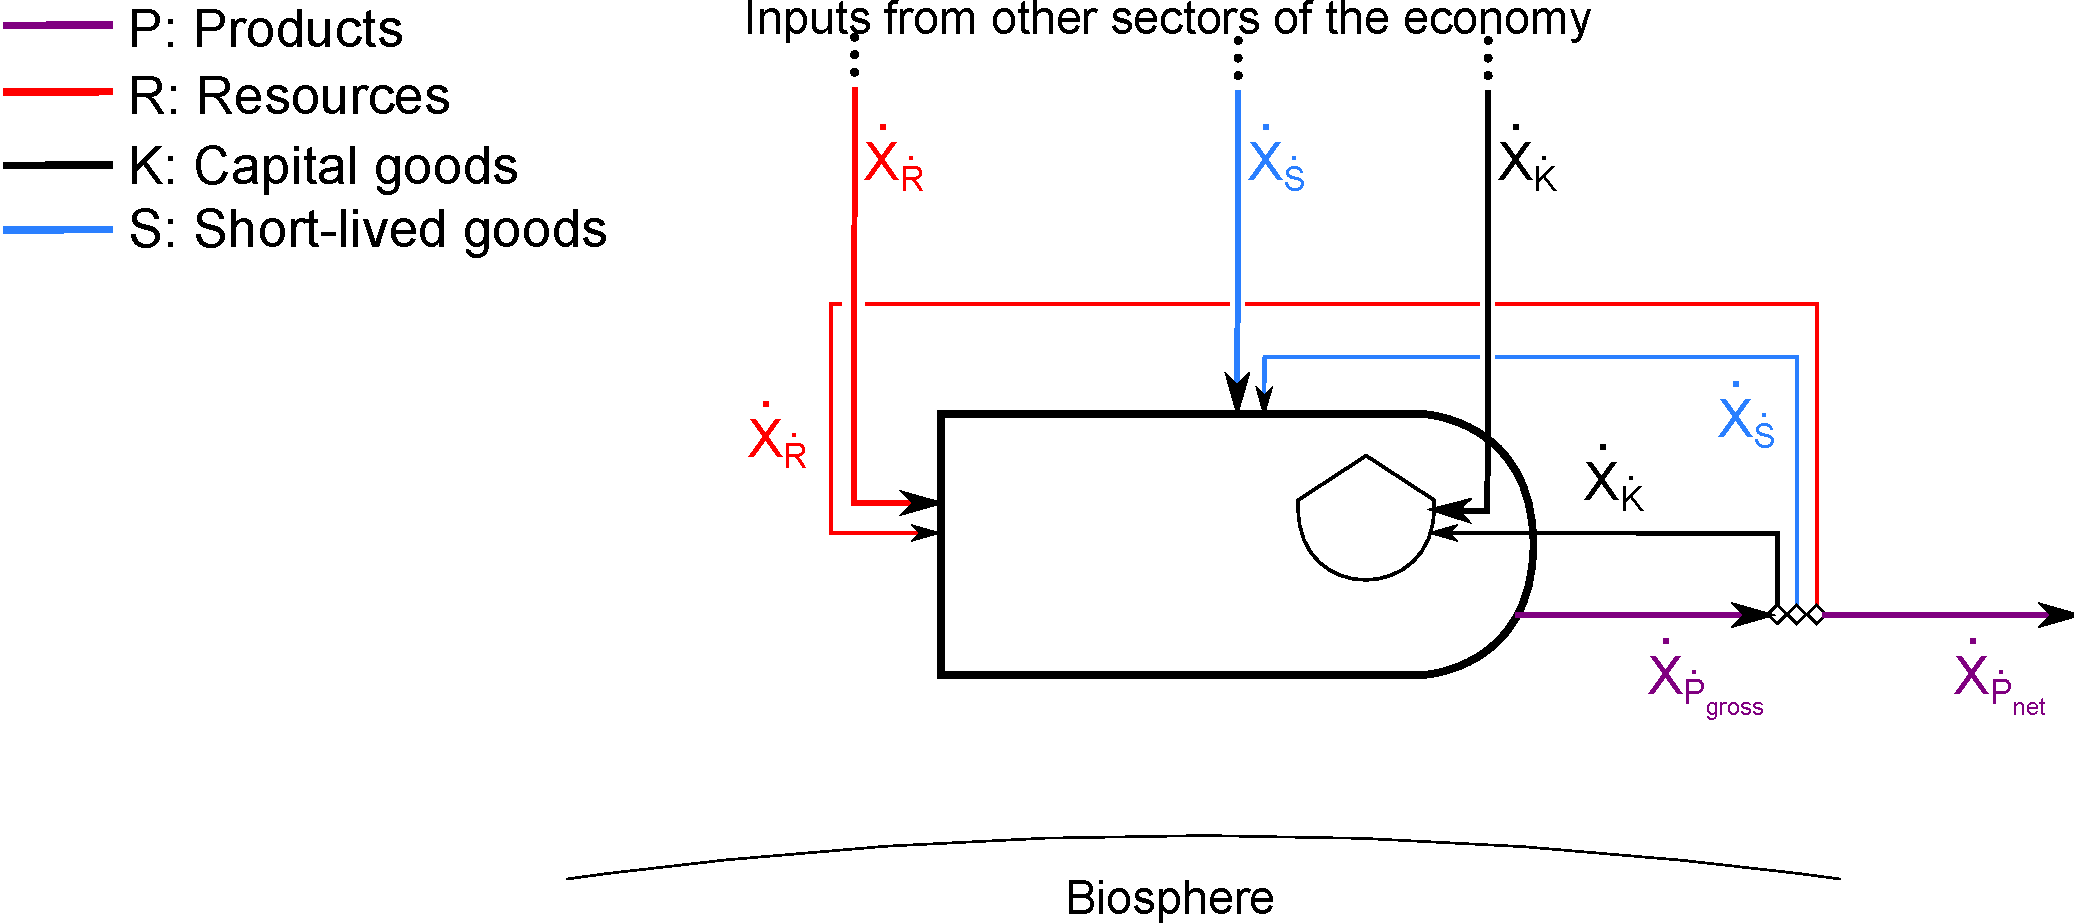
\includegraphics[width=\linewidth]{Part_2/Chapter_Values/images/PERKS_basic_unit_value_all.pdf}
\caption[Flows of value for a single sector]{Flows of value ($\dot{X}$) 
for a single sector. 
The value flows are associated with each of the different 
material and energy flows outlined in previous chapters.}
\label{fig:basic_value} 
\end{figure}

We denote creation and destruction
of value within a sector using the notion of ``source'' and ``sink.''
In Figure~\ref{fig:basic_value_aggregated}, the open circle, 
``source,'' inside the economic sector represents the value-added,
that is, the value that is created by the economic processes within that sector. 
The flows of value from a value-source are denoted $\dot{X}_{gen}$. 
Similarly, black circles represent the value ``sinks''  where value is destroyed 
by economic  processes or natural disasters. 
The flows of value into the value sinks are denoted $\dot{X}_{dest}$. 
Although we do not define 
the value creation and destruction processes any further (mathematically), 
we discuss what is meant by the
underlying processes in more detail below.

\begin{figure}[!ht]
\centering
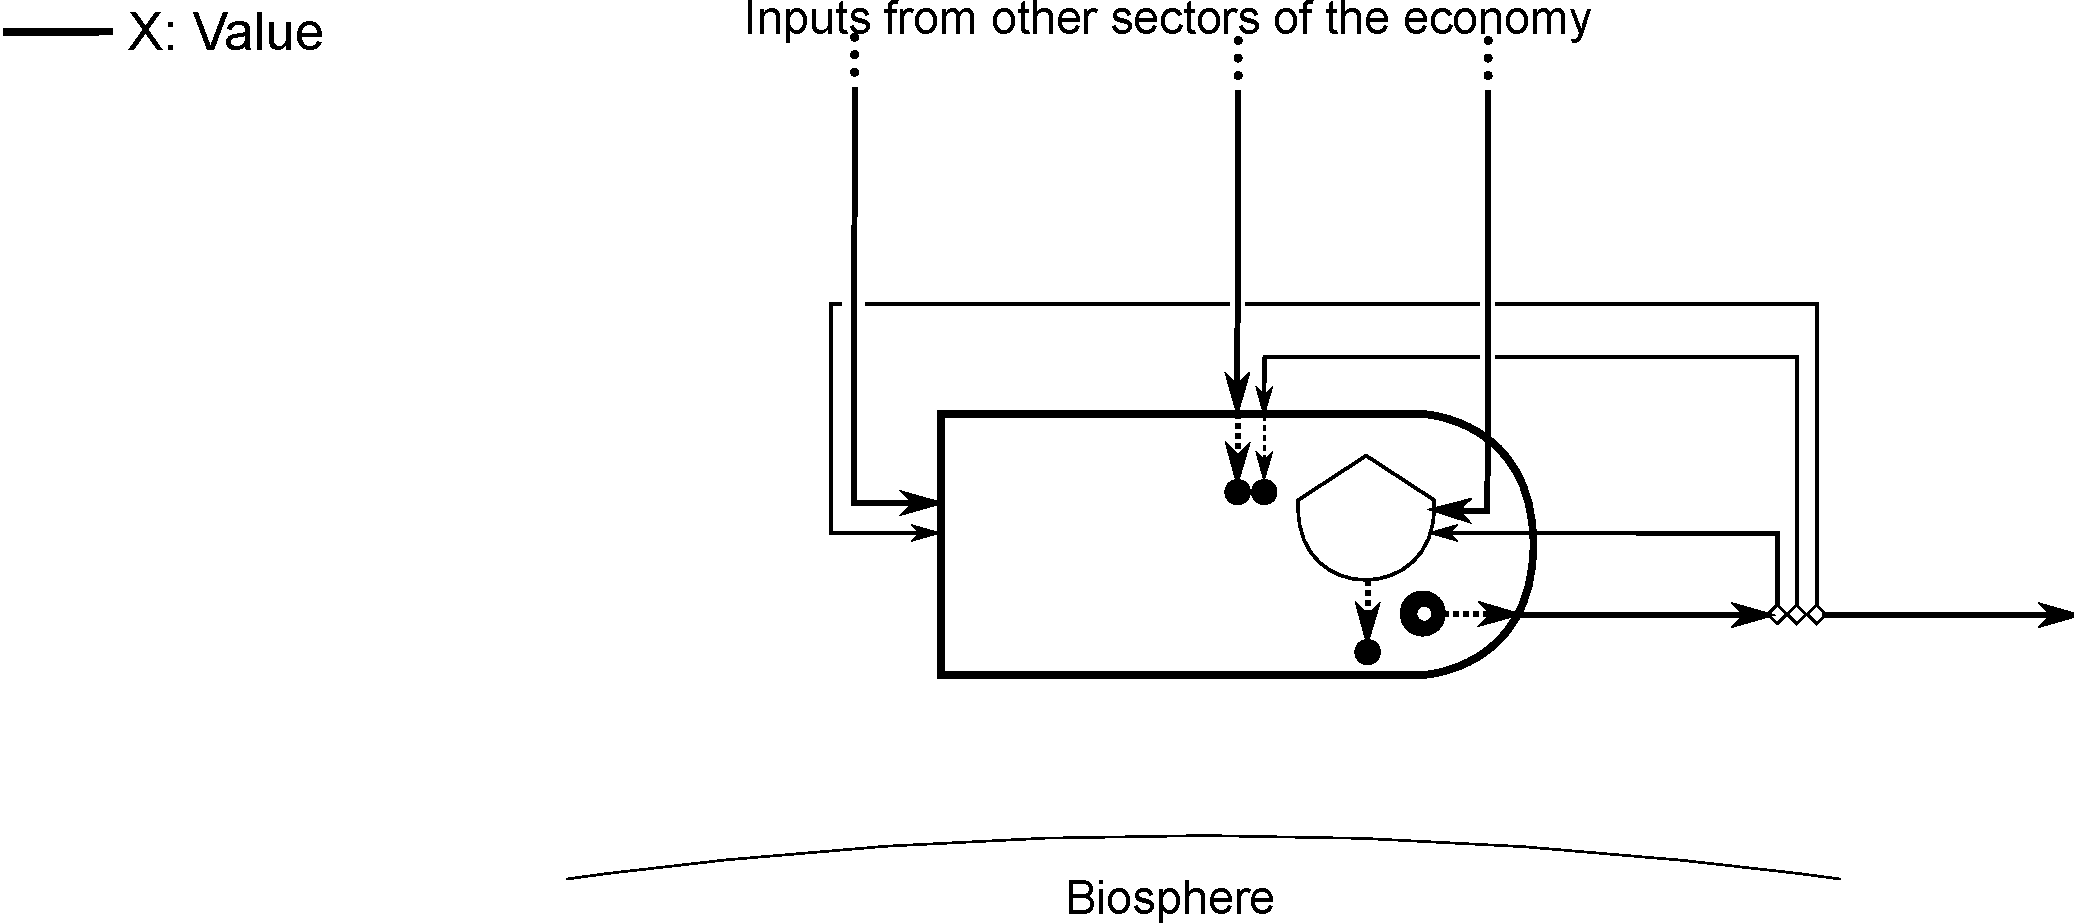
\includegraphics[width=\linewidth]{Part_2/Chapter_Values/images/PERKS_basic_unit_value.pdf}
\caption[Aggregated flows of value for a single sector]{Aggregated flows of value ($\dot{X}$) 
for a single sector. 
Distinction is made between value flows that 
enter the sector and are accumulated (i.e.\ capital goods) 
and value flows that are not accumulated. 
Within the sector there is destruction of value $\dot{X}_{dest}$, 
represented by the downward arrow flowing 
into the black sink and generation of value, 
represented by the arrow flowing out of a source. }
\label{fig:basic_value_aggregated} 
\end{figure}


%%%%%%%%%% Example A: single-sector economy %%%%%%%%%%
\section{Example A: single-sector economy} % chktex 13
\label{sec:value_example_A}
%%%%%%%%%%

Figure~\ref{fig:A_value} shows flows of value in the single-sector economy.
Following typical assumptions in economic modeling, 
the economy is \emph{completely isolated} from the biosphere
in terms of both material inputs and wastes.
In other words, the value flows of an economy are \emph{independent from}
material inputs and wastes.
Value flows are independent from material inputs,
because raw materials have no economic value 
until they have been removed from the biosphere by the extraction industry.
Value flows are independent from wastes,
because wastes, by definition, have no economic value 
upon leaving the economy.

\begin{landscape}
\begin{figure}[!ht]
\centering
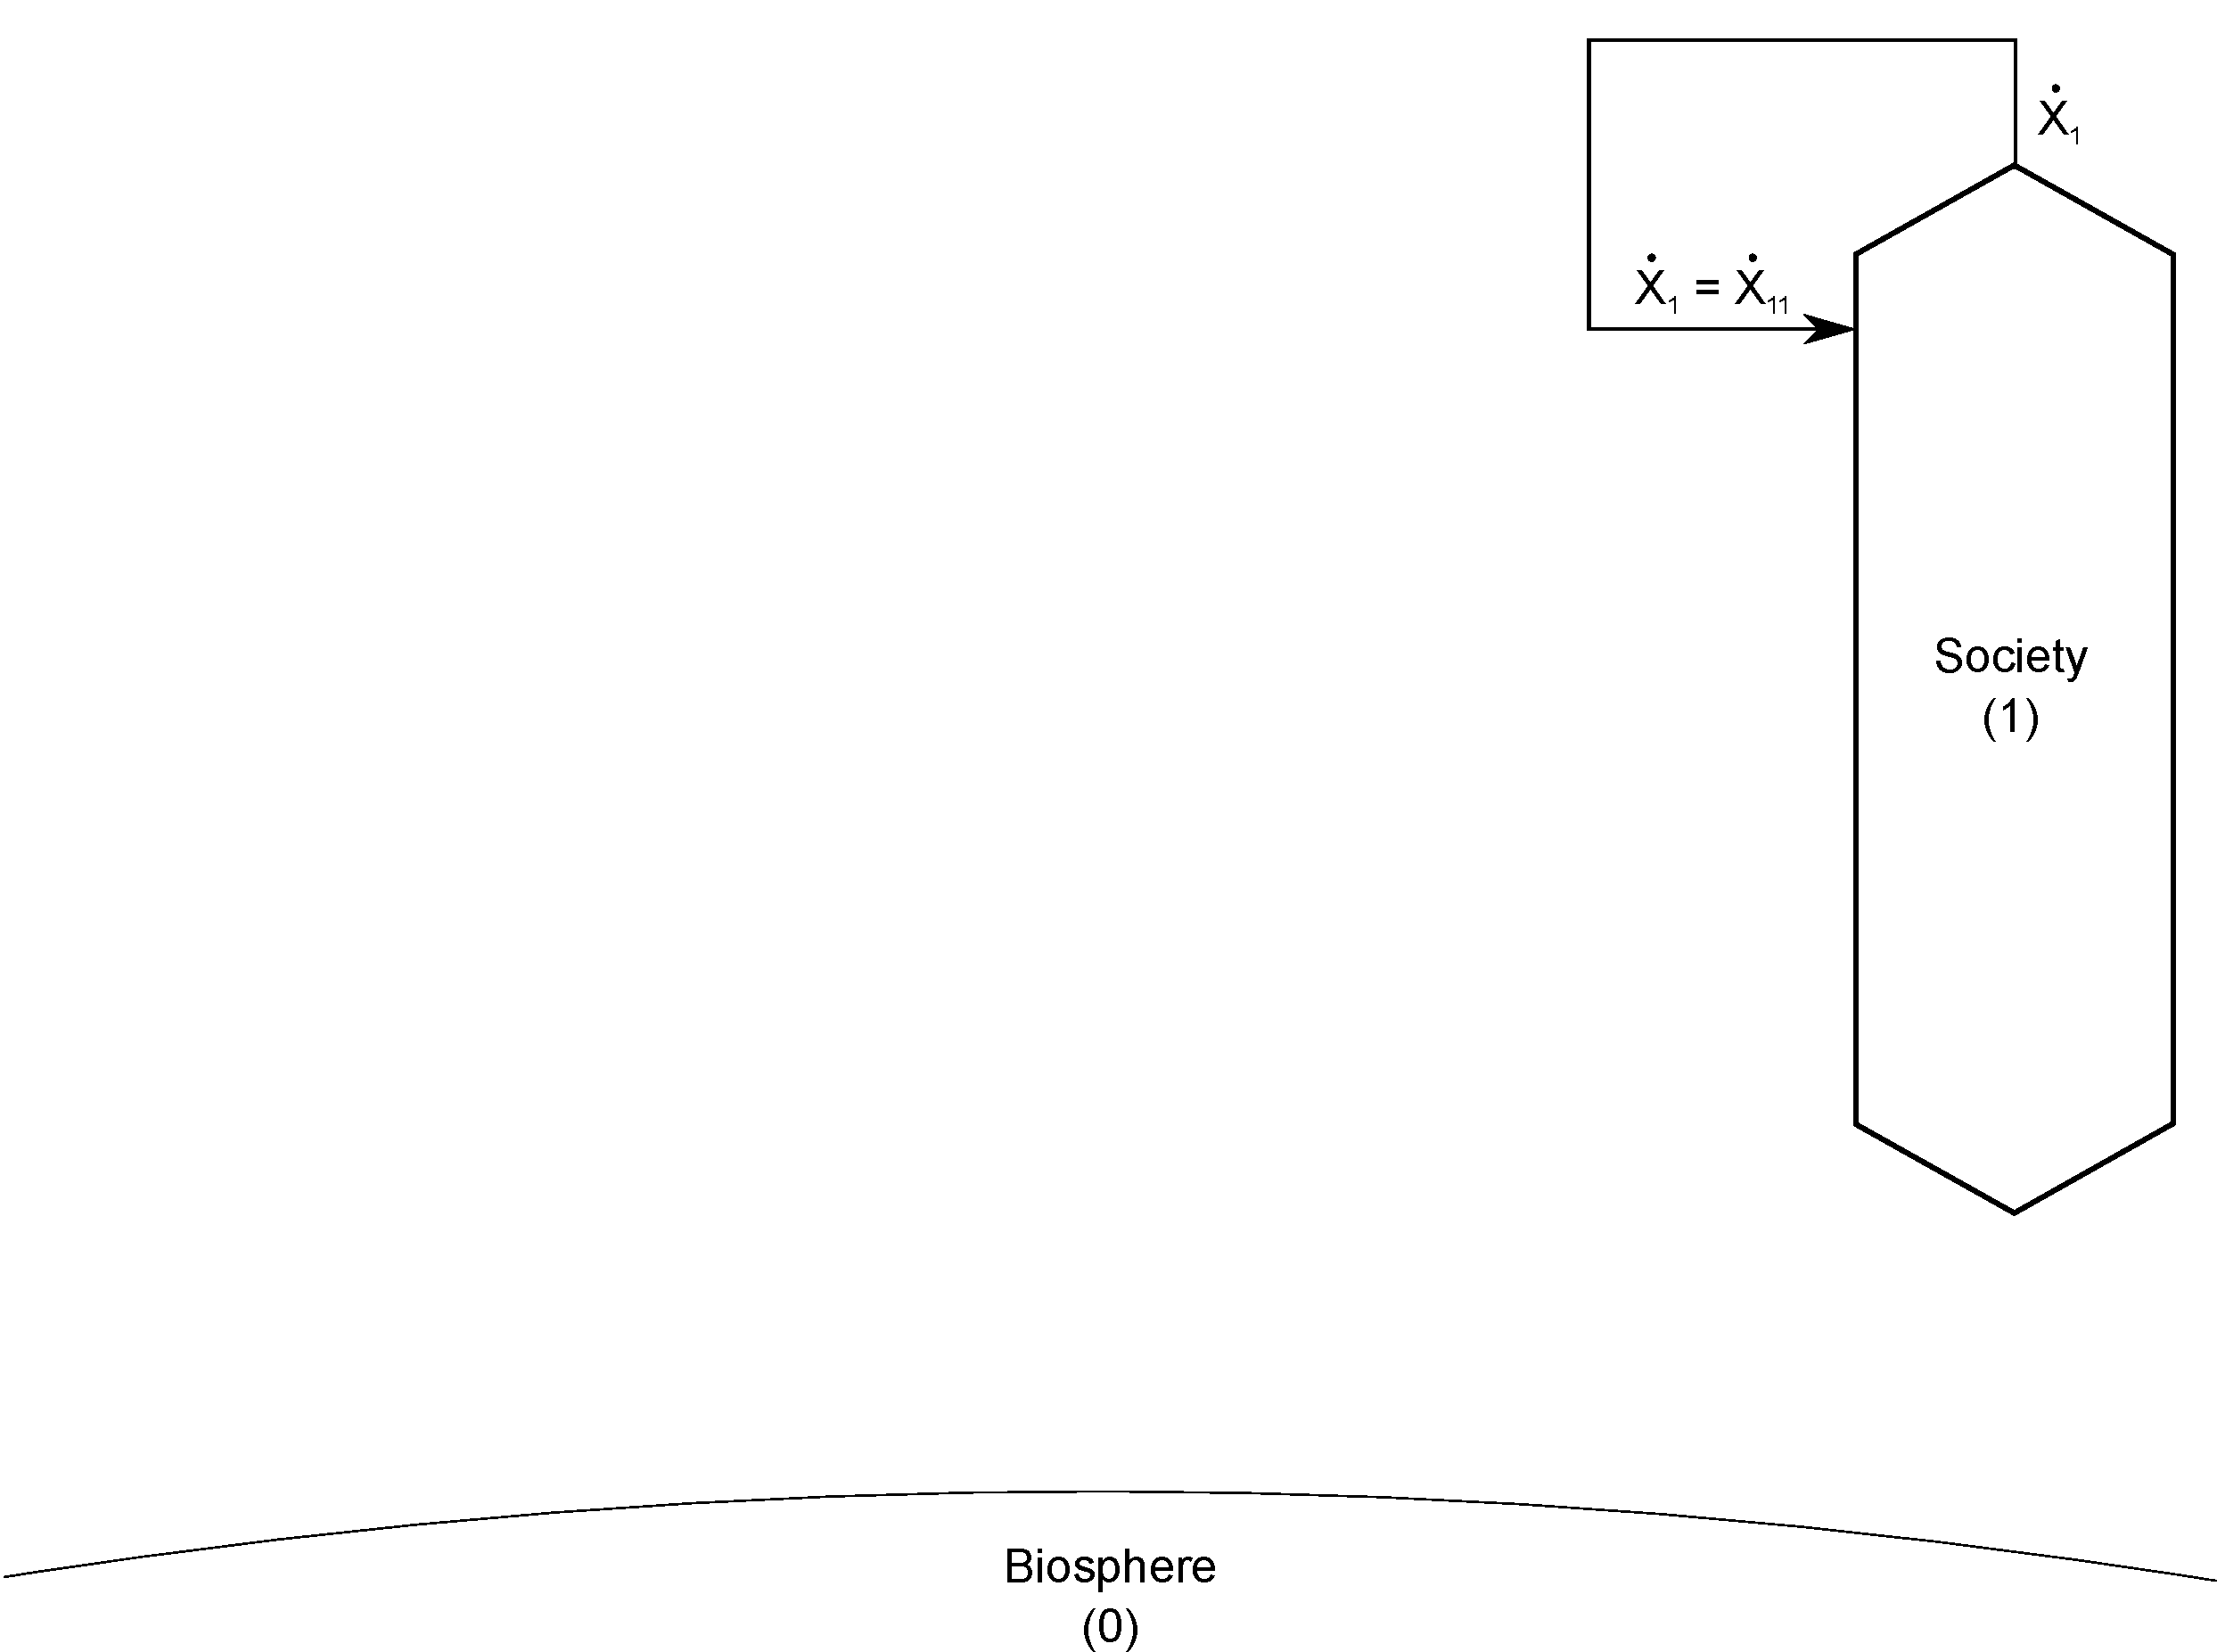
\includegraphics[width=0.8\linewidth]{Part_2/Chapter_Values/images/1_sector_value.pdf}
\caption[Flows of value for a one-sector economy]{Flows of value ($\dot{X}$) for a one-sector economy.}
\label{fig:A_value} 
\end{figure}
\end{landscape}

The contrast between the biophysical picture
(as represented in Figures~\ref{fig:A_materials} and~\ref{fig:A_energy})
on the one hand, 
and the conventional viewpoint of economics
(as represented in Figure~\ref{fig:A_value}) 
on the other, is striking.  
The biophysical picture of material and energy flows in 
Figures~\ref{fig:A_materials} and~\ref{fig:A_energy} 
emphasizes interaction with and dependence upon the biosphere 
that is not reflected in the typical economics representation of 
value flows depicted in Figure~\ref{fig:A_value}.
The isolation of the value flows from the biosphere is a consequence
of the subjective theory of value
that underpins modern economics.
The biosphere is akin to a third party with no voice 
in determining the value of a transaction:
it is neither buyer nor seller. 

Equation~\ref{eq:A_X_acct_1} describes the accumulation 
of value~($X$).
%
\begin{equation} \label{eq:A_X_acct_1}
	\frac{\mathrm{d}X_{1}}{\mathrm{d}t} 
	= \dot{X}_{11} 
	- \dot{X}_{1}
	+ \dot{X}_{gen,1}
	- \dot{X}_{dest,1}.
\end{equation}
%
The following subsections discuss the terms in Equation~\ref{eq:A_X_acct_1}.
%

%+++++++++ Example A: Economic Transactions ++++++++++
\subsection[Economic transactions]{Economic transactions ($\dot{X}_{11}$ and $\dot{X}_{1}$)}
%+++++++++

The returning arrow in Figure~\ref{fig:A_value} 
represents transactions between 
\begin{itemize}
	\item{buyers (who receive things of value, $\dot{X}_{11}$,
	in exchange for currency) and}
	\item{sellers (who give up things of value, $\dot{X}_{1}$,
	in exchange for currency).}
\end{itemize}

It is interesting to note that when a good is sold for more
than the producer paid for its inputs, 
the seller has created value and sold it into the economy. 
As a consequence, the seller's stock of currency grows,
providing the seller with an increased level of claim 
on value in the economy.

The subjective theory of value~(Section~\ref{sec:Value_Methodology})
posits that buyers and sellers agree on value at the 
time of the transaction.
Thus, $\dot{X}_{1} = \dot{X}_{11}$, and Equation~\ref{eq:A_X_acct_1}
simplifies to
%
\begin{equation} \label{eq:A_X_acct_2}	
	\frac{\mathrm{d}X_{1}}{\mathrm{d}t}	
	= \dot{X}_{gen,1}
	- \dot{X}_{dest,1},
\end{equation}
%
indicating that value accumulates in the economy
$\left( \frac{\mathrm{d}X_{1}}{\mathrm{d}t} \right)$
due to value generation ($\dot{X}_{gen,1}$) 
and destruction ($\dot{X}_{dest,1}$) processes only.


%+++++++++ Example A: value generation ++++++++++
\subsection[Value generation]{Value generation ($\dot{X}_{gen}$)}
%+++++++++

\noindent In Equation~\ref{eq:A_X_acct_1}, 
the value generation term ($\dot{X}_{gen}$) is akin to growing apples
in Section~\ref{sec:Materials_Methodology}: 
value is generated, seemingly out of nothing.
But, in fact, value is not created out of nothing. 
Rather, value is created from a variety of factors that have no apparent 
monetary cost to producers, including:
%
\begin{itemize}
	\item{flow of solar energy
	into the economy,
	as in the example of growing apples,}
	
	\item{extraction of resources (e.g., water, minerals, and
	fossil fuels) or any other unpriced goods from the biosphere, and}
	
	\item{exploitation of the unpriced waste assimilation capacity of the biosphere.}
\end{itemize}
%
The subjective theory of value indicates that 
there is no economic value associated with these ``transactions,'' 
because no currency is exchanged. 

The above factors indicate that the process of value generation
has both direct and indirect impacts on the biosphere.
The direct impacts are obvious: 
extraction of non-renewable resources from the biosphere, 
at rates greater than their natural accretion,
represents unsustainable overuse of natural capital.
The indirect impacts are less obvious: 
the value generated by these transactions can lead to increased wealth,
leading to increased demand rates for goods and services, 
whose production requires ever-increasing rates 
of unsustainable natural resource extraction.

As discussed in previous Chapters,
natural resource quality has a direct impact on both
material and energy intensity of economic processes.
As we extract lower quality resources, we require
larger inputs of materials and energy
to process greater volumes of material
and to build the extra capital equipment
necessary to do the extra processing.
This requires the allocation of a greater amount
of economic resources toward the primary production sectors.
In order to make profit,
these extra resources increase the value of the products
from these sectors,
to cover the added costs of production.
These impacts ripple through the economy 
increasing the costs of production in all downstream sectors.%
	\footnote{
	The issue 
	of resource quality will be discussed in more
	detail in Section~\ref{sec:resource_quality_and_irreversibility}.
	}

The term $\dot{X}_{gen}$ is accounted as ``value added'' to an industry in national accounts.
It is calculated as the difference between gross economic output of the industry
and the cost of its intermediate inputs.\cite{BEAVA}  
A simple way to think of value added is
the increase in value of the raw materials from the work performed 
on them by workers and manufactured capital.


%+++++++++ Example A: value destruction ++++++++++
\subsection[Value destruction]{Value destruction ($\dot{X}_{dest}$)}
%+++++++++

\noindent In Equation~\ref{eq:A_X_acct_1}, 
the value destruction term ($\dot{X}_{dest}$)
is akin to consuming apples: 
value is destroyed by a process that consumes, 
or otherwise renders unusable, 
previously-valuable things in the economy
(see Section~\ref{sec:Materials_Methodology}).
The factors that lead to value destruction
($\dot{X}_{dest}$) include:
%
\begin{itemize}
	\item{depreciation, usually associated with disposal of 
	materials and equipment to the biosphere at end of life and}
	\item{natural disasters, such as hurricanes and typhoons,
	that destroy equipment and property.}
\end{itemize}

$\dot{X}_{dest}$ is accounted as depreciation, 
or ``consumpton of fixed capital,'' % chktex 38
to an industry in the national accounts. 
It is a monetary estimate of the physical effects on assets from 
``wear and tear, obsolescence, accidental damage,
and aging.''~\cite{katz2008} 


%+++++++++ Example A: GDP and Stock of Value ++++++++++
\subsection{GDP}
%+++++++++

If Society (1) in Figure~\ref{fig:A_value} represents 
the economy of an entire country, 
$\dot{X}_{1}$ is its gross domestic product (GDP)
in units of \$/year. 
GDP is a flow, not a stock. 
GDP is often considered a stock, but that is incorrect. 
$X_{1}$ is a stock, akin to monetary wealth. 
However, $X_{1}$ is a very
narrow definition of wealth
that neglects the value of natural resources, 
the value of social captial, and any
other ``wealth'' that cannot be exchanged for money. 


%%%%%%%%%% Example B: two-sector economy %%%%%%%%%%
\section{Example B: two-sector economy} % chktex 13
%%%%%%%%%%

Figure~\ref{fig:B_value} shows flows of value ($\dot{X}$) 
within a two-sector economy. 
Again, we note the isloation of economic value from the biosphere.

\begin{landscape}
\begin{figure}[!ht]
\centering
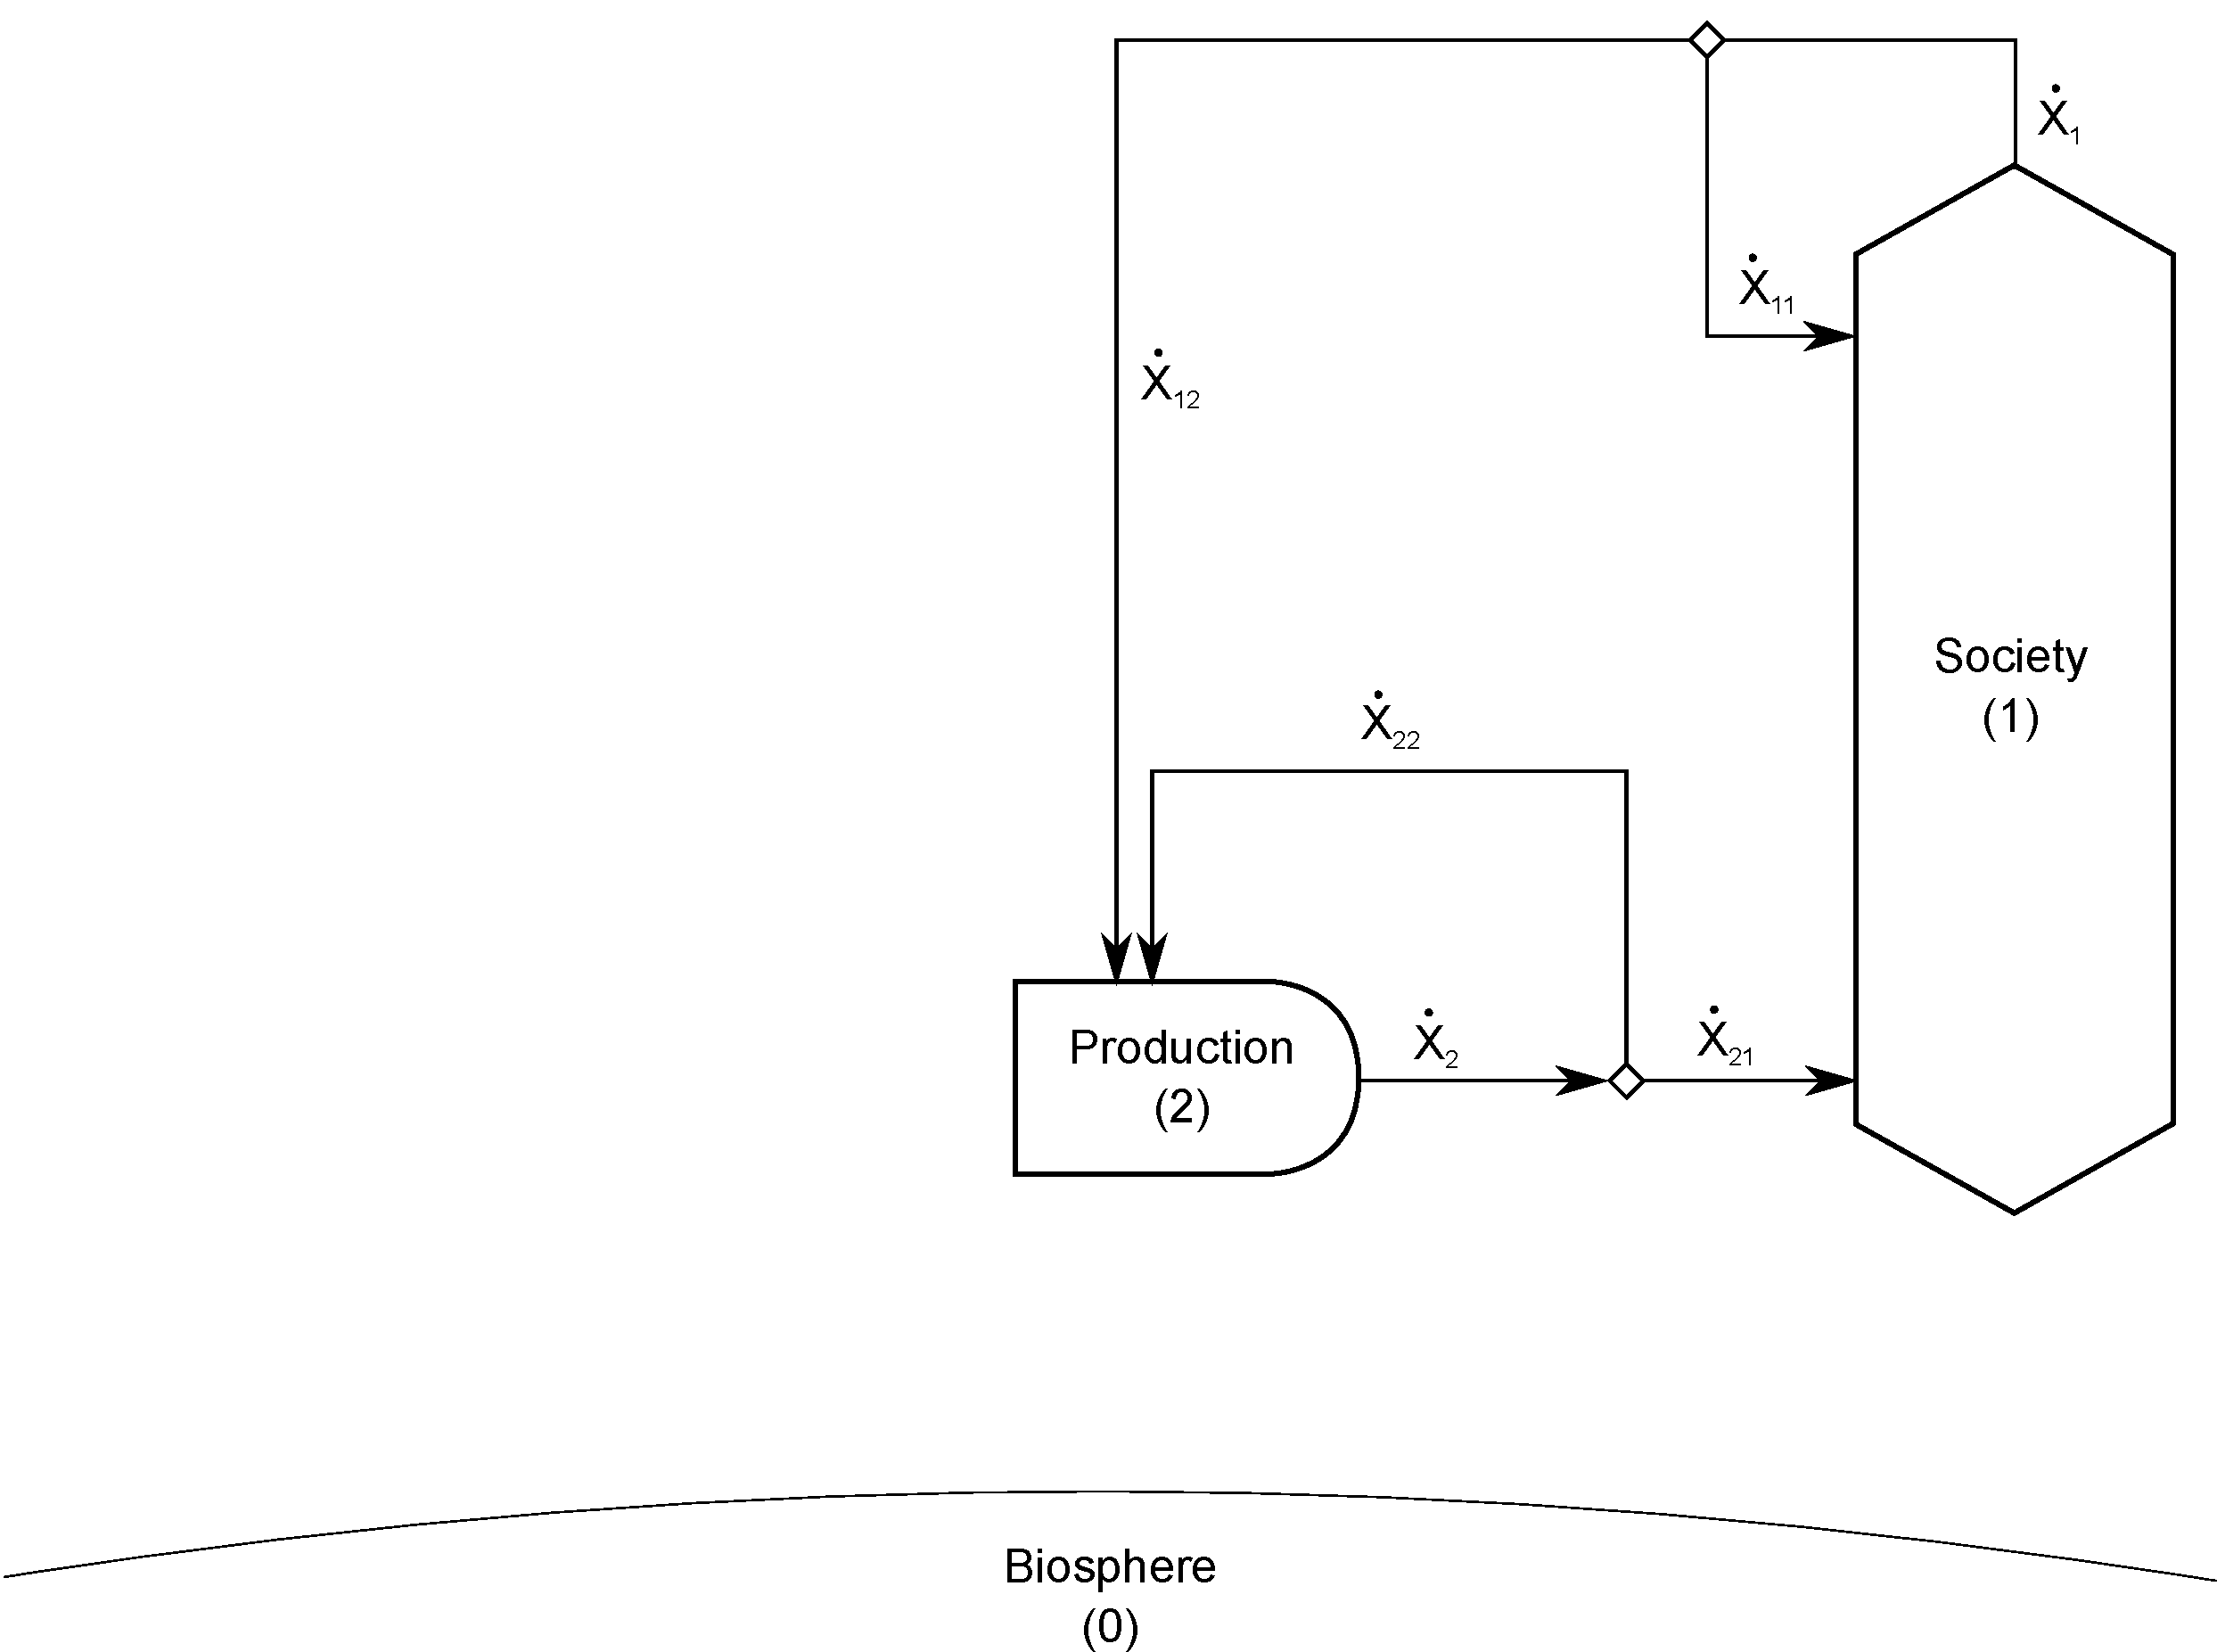
\includegraphics[width=0.8\linewidth]{Part_2/Chapter_Values/images/2_sector_value.pdf}
\caption[Flows of value within a two-sector economy]{Flows of value ($\dot{X}$) within a two-sector economy.}
\label{fig:B_value}
\end{figure}
\end{landscape}

We can account for value flows by writing
the following equations:
%
\begin{equation}\label{eq:B-value-1}
	\frac{\mathrm{d}X_{1}}{\mathrm{d}t}
	= \dot{X}_{11}
	+ \dot{X}_{21}
	- \dot{X}_{1}
	+ \dot{X}_{gen,1}
	- \dot{X}_{dest,1}
\end{equation}
%
and
%
\begin{equation}\label{eq:B-value-2}
	\frac{\mathrm{d}X_{2}}{\mathrm{d}t}
	= \dot{X}_{12}
	+ \dot{X}_{22}
	- \dot{X}_{2}
	+ \dot{X}_{gen,2}
	- \dot{X}_{dest,2}.
\end{equation}

Equations~\ref{eq:B-value-1} and~\ref{eq:B-value-2}
can be generalized as
%
\begin{equation}\label{eq:B-value-generalized}
	\frac{\mathrm{d}X_{j}}{\mathrm{d}t}
	= \sum\limits_{i=1}^n \dot{X}_{ij}
	- \dot{X}_{j}
	+ \dot{X}_{gen,j}
	- \dot{X}_{dest,j},
\end{equation}
%
where $n$ is the number of sectors in the economy, and $j \in [1, n]$.


%%%%%%%%%% Example C: three-sector economy %%%%%%%%%%
\section{Example C: three-sector economy} % chktex 13
\label{sec:value_example_C}
%%%%%%%%%%

Figure~\ref{fig:C_value} shows flows of value ($\dot{X}$) 
within a three-sector economy. 

\begin{landscape}
\begin{figure}[!ht]
\centering
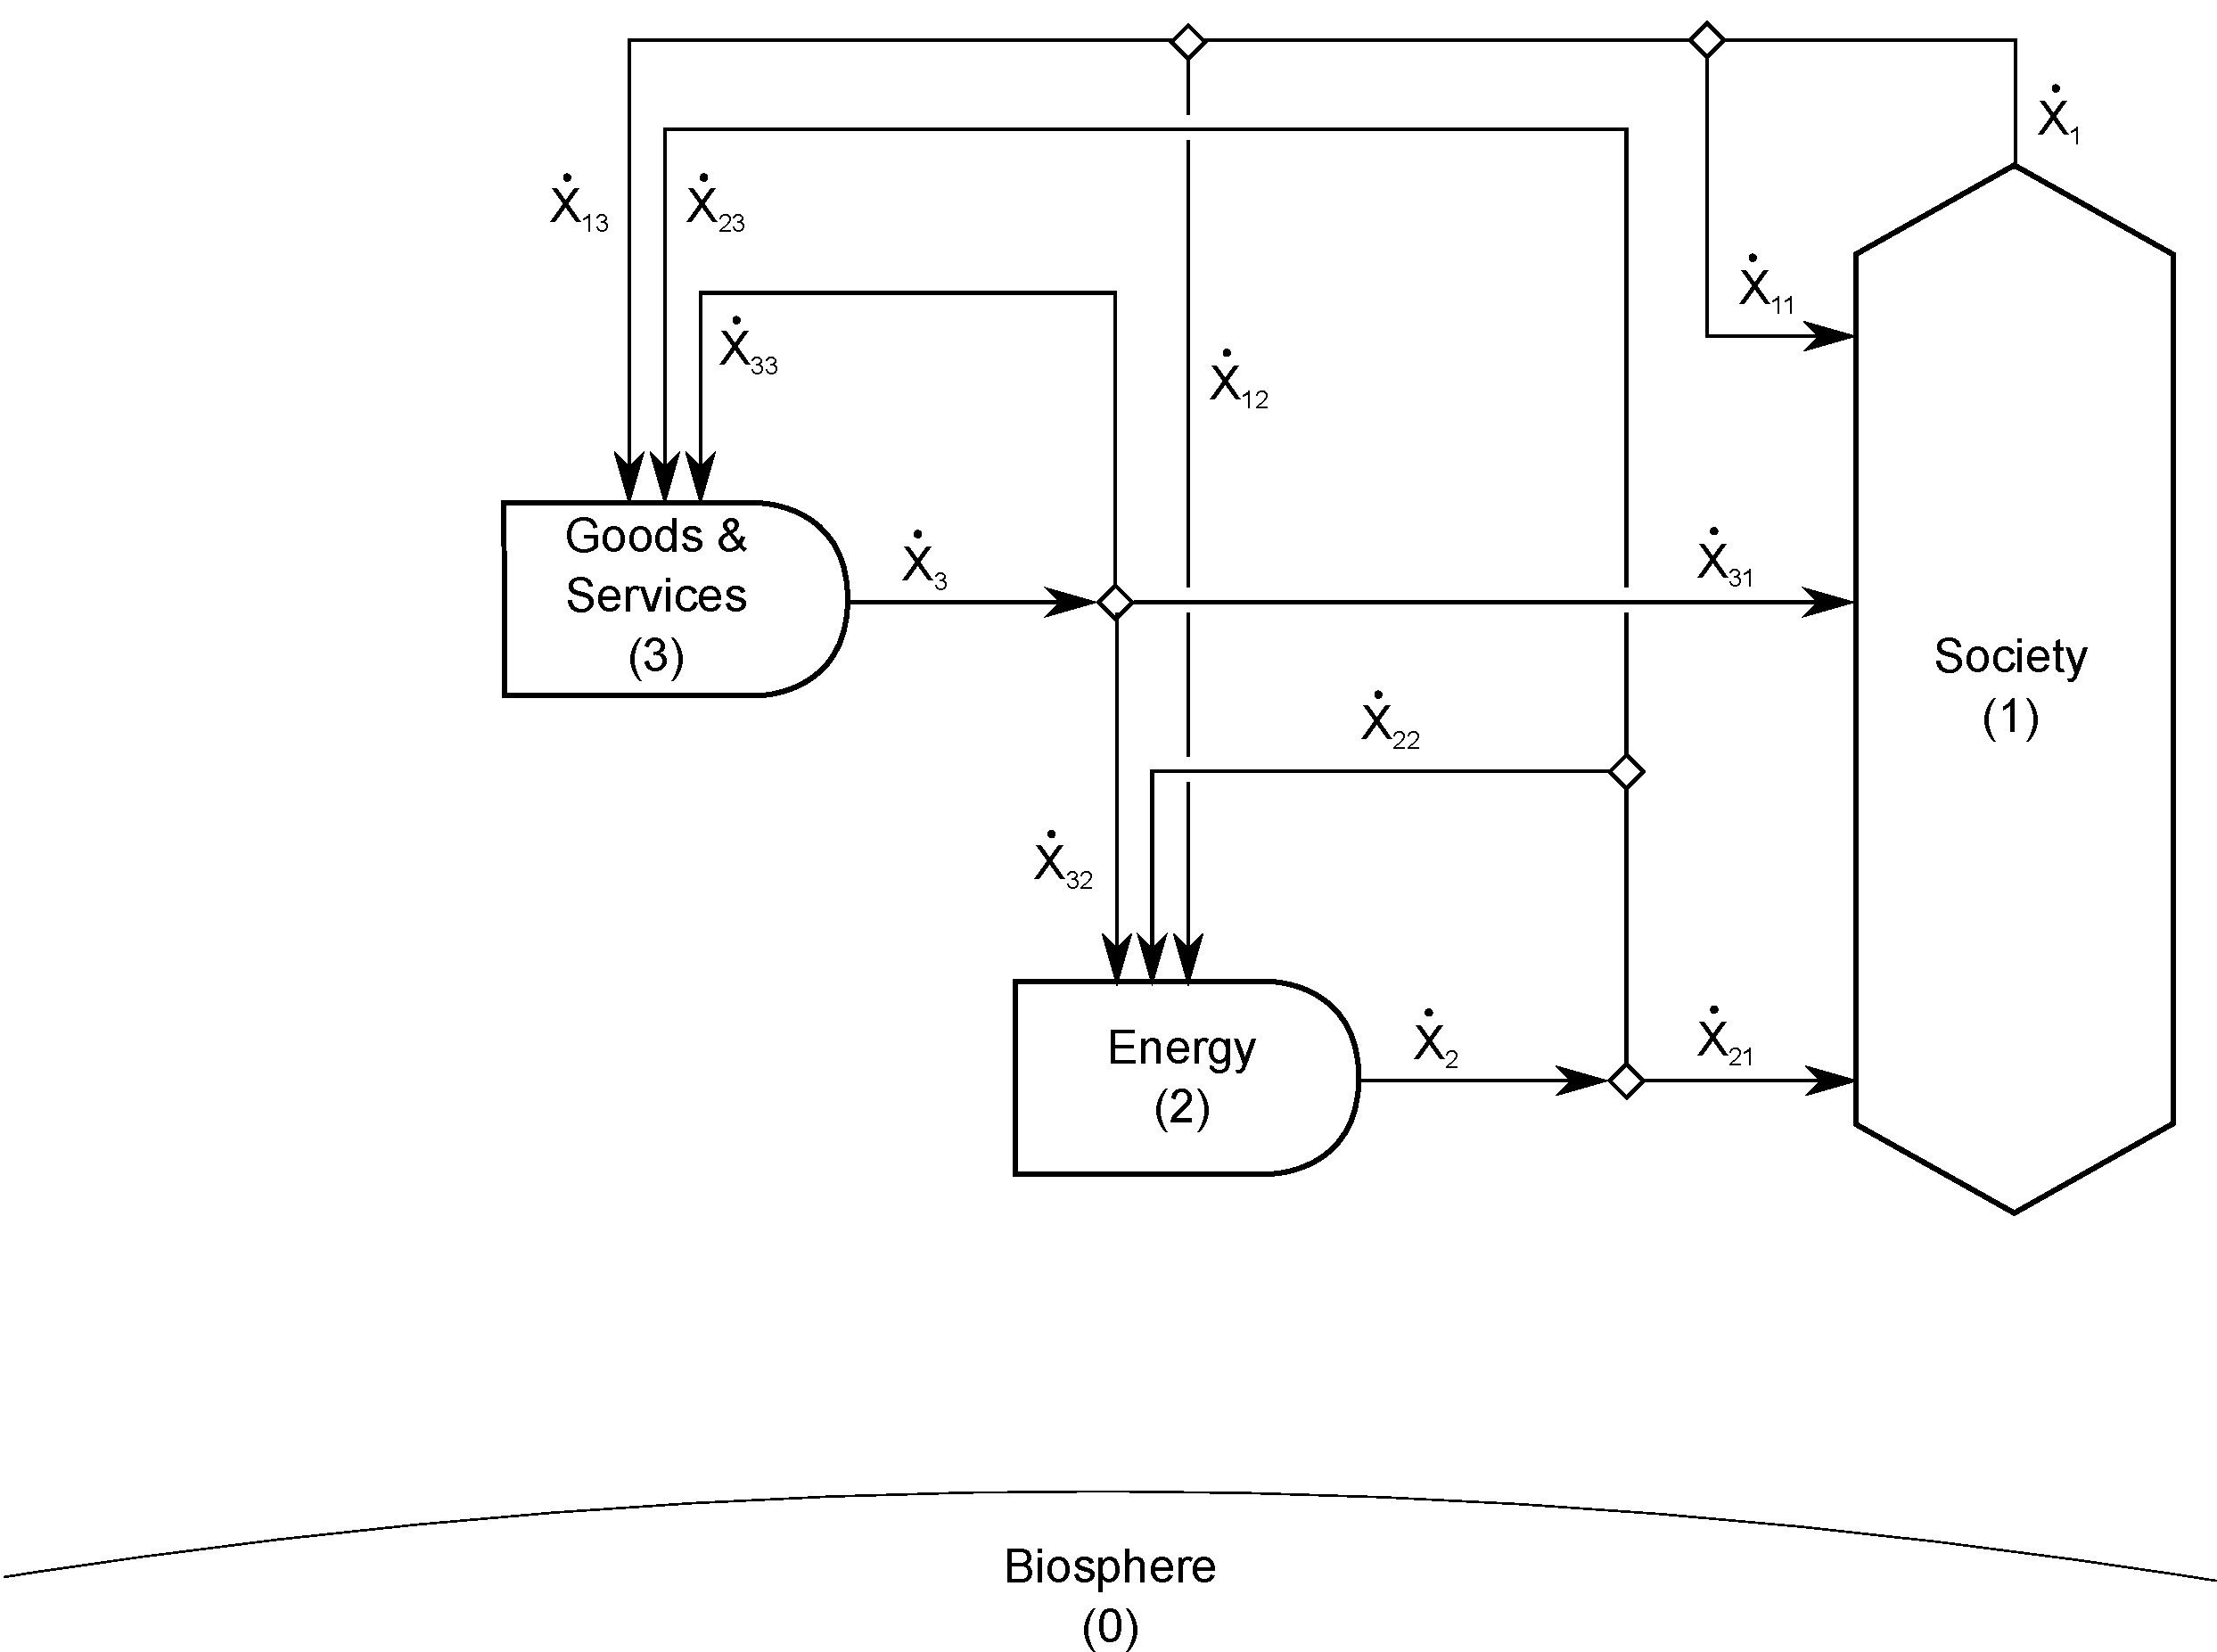
\includegraphics[width=0.8\linewidth]{Part_2/Chapter_Values/images/3_sector_value.pdf}
\caption[Flows of value within a three-sector economy]{Flows of value ($\dot{X}$) within a three-sector economy.}
\label{fig:C_value}
\end{figure}
\end{landscape}

The equations representing flows of value in Example~C are:
%
\begin{equation}\label{eq:C-value-generalized}
	\frac{\mathrm{d}X_{j}}{\mathrm{d}t}
	= \sum\limits_{i=1}^{n} \dot{X}_{ij}
	- \dot{X}_{j}
	+ \dot{X}_{gen,j}
	- \dot{X}_{dest,j},
\end{equation}
%
where $n$ is the number of sectors in the economy, and $j \in [1, n]$.
Equation~\ref{eq:C-value-generalized} is identical to Equation~\ref{eq:B-value-generalized}.
If we sum the value accounting equations for the entire economy, 
we obtain
%
\begin{equation}\label{eq:C-value-economy-a}
	\sum\limits_{j=1}^{n} \frac{\mathrm{d}X_{j}}{\mathrm{d}t}
	= \sum\limits_{j=1}^{n} \sum\limits_{i=1}^{n} \dot{X}_{ij}
	- \sum\limits_{j=1}^{n} \dot{X}_{j}
	+ \sum\limits_{j=1}^{n} \dot{X}_{gen,j}
	- \sum\limits_{j=1}^{n} \dot{X}_{dest,j}.
\end{equation}
%
With the identities
%
\begin{equation} \label{eq:X_identity_1}
	\dot{X}_{j}  
	= \sum\limits_{k=1}^n \dot{X}_{jk}
\end{equation}
%
and
%
\begin{equation} \label{eq:X_identity_2}
	\sum\limits_{j=1}^n\dot{X}_{j}  
	= \sum\limits_{j=1}^n \sum\limits_{k=1}^n \dot{X}_{jk}
	= \sum\limits_{i=1}^n \sum\limits_{k=1}^n \dot{X}_{ik}
	= \sum\limits_{i=1}^n \sum\limits_{j=1}^n \dot{X}_{ij}
	= \sum\limits_{j=1}^n \sum\limits_{i=1}^n \dot{X}_{ij},
\end{equation}
%
Equation~\ref{eq:C-value-economy-a} becomes
%
\begin{equation}\label{eq:C-value-economy-b}
	\sum\limits_{j=1}^{n} \frac{\mathrm{d}X_{j}}{\mathrm{d}t}
	= \sum\limits_{j=1}^{n} \dot{X}_{gen,j}
	- \sum\limits_{j=1}^{n} \dot{X}_{dest,j},
\end{equation}
%
for $j \in [1, n]$, indicating that 
value generation ($\dot{X}_{gen,j}$) 
and destruction ($\dot{X}_{dest,j}$)
are the only mechanisms by which value is accumulated or lost
$\left( \frac{\mathrm{d}X_{j}}{\mathrm{d}t} \right)$
within the economy.  
Equation~\ref{eq:C-value-economy-b} is a mathematical representation of the
value-added approach to measuring GDP\@. The sum of the
value-added across all industries is equivalent to the 
total value of final produced goods.\cite[p.~196]{Landefeld:2008aa}


%%%%%%%%%% Value: Auto industry example %%%%%%%%%%
\section{Value in the US auto industry}
\label{sec:value_auto}
%%%%%%%%%%

To estimate value flows through the automobile industry, 
we use publicly available data from the 
US BEA.\footnote{A 
	primer on using the US BEA
	industry data can be found 
	on the BEA website.\cite{Streitwieser:2011aa}}
The  tables needed to estimate dynamic 
value flows and capital accumulation within the economy 
are primarily the KLEMS\footnote{KLEMS is an acronym for 
	capital~(K), labor~(L), energy~(E), materials~(M), and services~(S).} 
Intermediate Use
tables and 
the fixed asset, non-residential detail table. 
The KLEMS data tables
are based on the Input-Output (I-O) tables, 
but are at a lower level of aggregation and the inputs are categorized 
into three broad types: energy, materials, and services.

The KLEMS intermediate use data are categorized in the same
way as the input flows on the PERKS diagram. 
The total material inputs into the auto industry (IOC 3361MV) 
represents the value of resource flows ($\dot{X}_{\dot{R}}$). 
Similarly, the total direct energy inputs into the 
auto industry represents the value of energy flows ($\dot{X}_{\dot{E}}$),
and the total service inputs into the auto industry represents 
Short-lived goods ($\dot{X}_{\dot{S}}$).
The fixed asset accounts are
used to estimate capital value flows 
($\dot{X}_{\dot{K}}$) as well as self-use of capital.  
The I-O tables are used to determine gross economic output of the 
auto industry ($\dot{X}_{\dot{P}_{Gross}}$). And subtracting self-use capital and resources
from Gross Economic Output yields Net Economic Output ($\dot{X}_{\dot{P}_{net}}$).

Using these data, Figure~\ref{fig:PERKS_value_auto_ind} provides estimates 
of value flows for the US auto industry.
Table~\ref{tab:data} contains a brief summary  
of the data sources that were used 
to obtain the values in Figure~\ref{fig:PERKS_value_auto_ind}. 
Appendix~\ref{chap:auto_value_flows} contains
detailed calculations and sources of data.

\begin{landscape}
\begin{figure}[!ht]
\centering
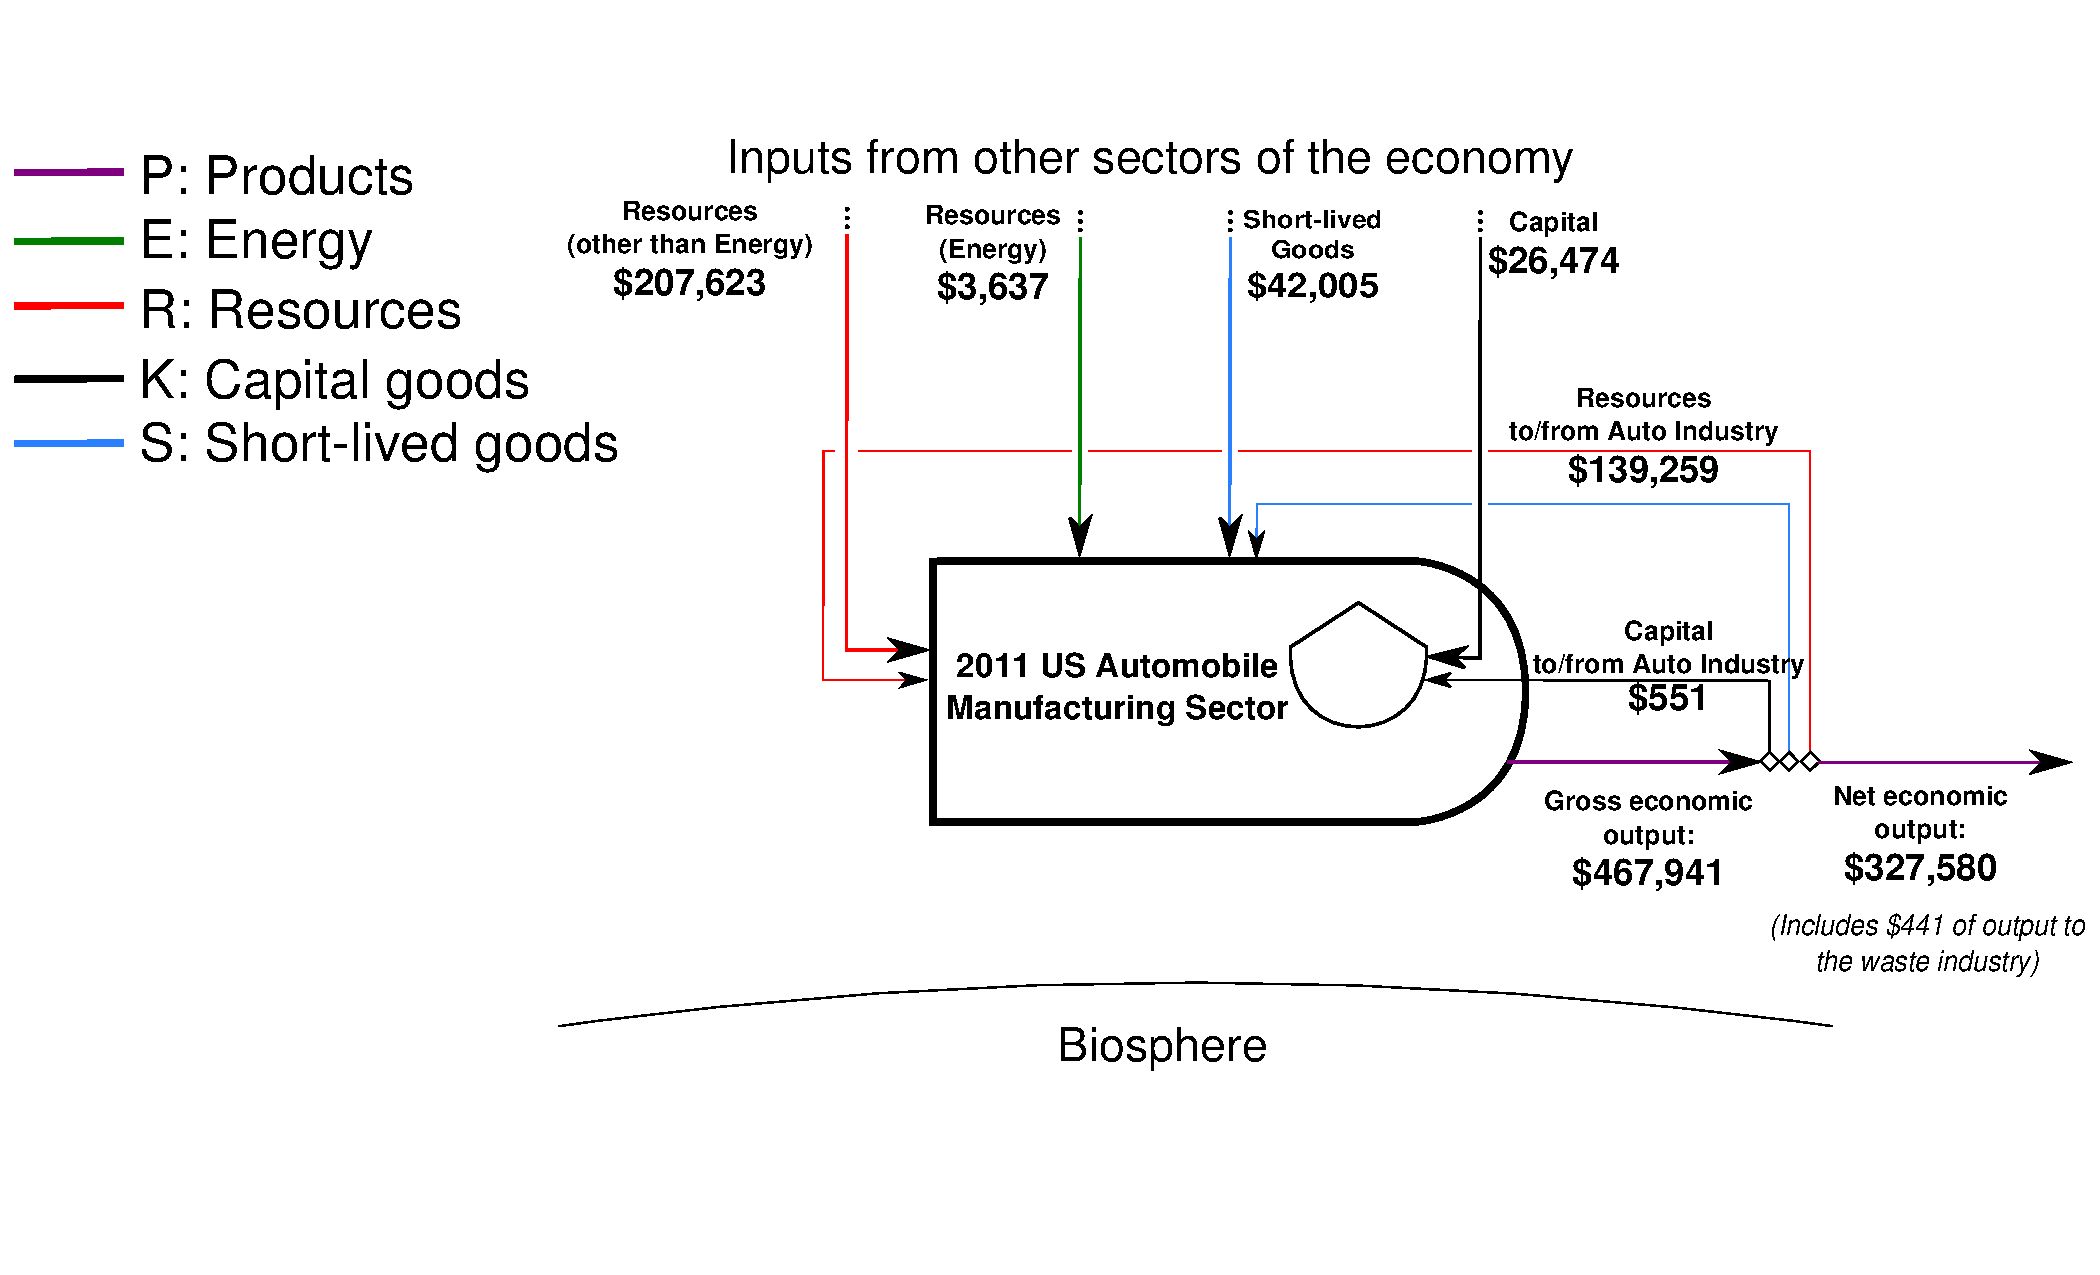
\includegraphics[width=0.8\linewidth]{Part_2/Chapter_Values/images/PERKS_basic_unit_value_auto_ind.pdf}
\caption[Value of material and energy flows 
into and out of the US automobile industry]{Value 
of material and energy flows into and out of the 
US automobile industry (in millions of 2011USD).}
\label{fig:PERKS_value_auto_ind}
\end{figure}
\end{landscape}

\begin{table}
\caption[Data Sources for auto industry (IOC 3361MV) example]{Data sources for auto industry (IOC 3361MV) example.}
\begin{center}
  \begin{tabular}{l r @{\hspace{2em}} l}
   \toprule 
     & 2011 USD &   \\ 
Value Flow & (millions) & BEA Data Source \\
	\midrule
    Resources  & \$175,491           & 2011 KLEMS Total Material Inputs \\

   Energy &   3,637&   2011 KLEMS Total Energy Inputs                \\

    Short-lived Goods &   74,578 &   2011 KLEMS Total Services Inputs    \\
%&&\\
    Capital &  15,447  &  2011 Fixed Assets 2011 (non-residential detailed estimates)     \\  

%&&\\
    Gross Economic Output & 482,269  &   2011 Input-Output Use Tables \\

%&&\\
    Resources (self-use)  &  133,961 & 2011 Input-Output Use Tables     \\
%&&\\
    Capital (self-use) & 15,181 & 2011 Fixed Assets (non-residential detailed estimates)      \\
%&&\\
    Net Economic Output & 333,127   &  Author's calculations \\
    \bottomrule
  \end{tabular}

\end{center}
\label{tab:data}
\end{table}


%%%%%%%%%% Value: Summary %%%%%%%%%%
\section{Summary}
\label{sec:value_summary}
%%%%%%%%%%

In this chapter, we developed techniques to account for flows of economic value
($\dot{X}$) through economies 
(Section~\ref{sec:Value_Methodology}).
We began with a discussion about theories of value and settled on
the prevailing subjective theory of value for our framework.
Thereafter, value accounting equations were developed and applied to example
economies~A--C % chktex 8
in Sections~\ref{sec:value_example_A}--\ref{sec:value_example_C}. 
We noted the need for terms that describe creation and destruction
of value ($\dot{X}_{gen}$ and $\dot{X}_{dest}$, respectively) 
within economic sectors.
Finally, we explored value flows 
to and from the US auto economy (Section~\ref{sec:value_auto}).

It is important to note at this point that, in contrast to materials and energy,
we found that there is no lack of data on value flows
to and from industry sectors available 
from the BEA. The value flows
are relatively easily derived from the 
data captured at the point of sale in market transactions. 
However, the BEA has no values for material and energy flows \emph{ to and from the biosphere}.
Ironically, the data on the physical flows of materials and energy
to and from the biosphere \emph{are} captured, by
 agencies such as the EPA and the EIA in the US and the IEA internationally.  
The challenge for national accounting arises when
trying to place a value on those flows. 
These challenges were taken up by
the UN starting in 1991. The comprehensive and rigorous UN System of Environmental Economic Accounts (SEEA)
is now in its third edition
and several European Union member states, as well as  the Phillipines, Canada, and  Austrailia, use
the SEEA
 to regularly account value flows to and from the biosphere
as part of their national accounts.
However, as recounted in the Prologue,  the US BEA has been politically
prevented from pursuing valuation of material and energy
flows to and from the biosphere ever since their 
first publication
of them in 1994.

In Chapter~\ref{chap:intensity}, 
we combine results from Chapters~\ref{chap:direct_energy}, 
\ref{chap:embodied_energy}, and~\ref{chap:value}
to develop techniques the estimate the energy intensity
of economic products.


\bibliographystyle{unsrt}
\bibliography{../../Metabolic}



% Always give a unique label
% and use \ref{<label>} for cross-references
% and \cite{<label>} for bibliographic references
% use \sectionmark{}
% to alter or adjust the section heading in the running head
%% Instead of simply listing headings of different levels we recommend to let every heading be followed by at least a short passage of text. Furtheron please use the \LaTeX\ automatism for all your cross-references and citations.

%% Please note that the first line of text that follows a heading is not indented, whereas the first lines of all sequent paragraphs are.

%% Use the standard \verb|equation| environment to typeset your equations, e.g.
%
%% \begin{equation}
%% a \times b = c\;,
%% \end{equation}
%
%% however, for multiline equations we recommend to use the \verb|eqnarray|
%% environment\footnote{In physics texts please activate the class option \texttt{vecphys} to depict your vectors in \textbf{\itshape boldface-italic} type - as is customary for a wide range of physical jects.}.
%% \begin{eqnarray}
%% a \times b = c \nonumber\\
%% \vec{a} \cdot \vec{b}=\vec{c}
%% \label{eq:01}
%% \end{eqnarray}

%% \section{section Heading}
%% \label{sec:2}
%% Instead of simply listing headings of different levels we recommend to let every heading be followed by at least a short passage of text. Furtheron please use the \LaTeX\ automatism for all your cross-references\index{cross-references} and citations\index{citations} as has already been described in Sect.~\ref{sec:2}.

%% \begin{quotation}
%% Please do not use quotation marks when quoting texts! Simply use the \verb|quotation| environment -- it will automatically render Springer's preferred layout.
%% \end{quotation}


%% \section{section Heading}
%% Instead of simply listing headings of different levels we recommend to let every heading be followed by at least a short passage of text. Furtheron please use the \LaTeX\ automatism for all your cross-references and citations as has already been described in Sect.~\ref{sec:2}, see also Fig.~\ref{fig:1}\footnote{If you copy text passages, figures, or tables from other works, you must obtain \textit{permission} from the copyright holder (usually the original publisher). Please enclose the signed permission with the manucript. The sources\index{permission to print} must be acknowledged either in the captions, as footnotes or in a separate section of the book.}

%% Please note that the first line of text that follows a heading is not indented, whereas the first lines of all sequent paragraphs are.

% For figures use
%
%% \begin{figure}[b]
%% \sidecaption
% Use the relevant command for your figure-insertion program
% to insert the figure file.
% For example, with the option graphics use
%% \includegraphics[scale=.65]{figure}
%
% If not, use
%\picplace{5cm}{2cm} % Give the correct figure height and width in cm
%
%% \caption{If the width of the figure is less than 7.8 cm use the \texttt{sidecapion} command to flush the caption on the left side of the page. If the figure is positioned at the top of the page, align the sidecaption with the top of the figure -- to achieve this you simply need to use the optional argument \texttt{[t]} with the \texttt{sidecaption} command}
%% \label{fig:1}       % Give a unique label
%% \end{figure}


%% \paragraph{Paragraph Heading} %
%% Instead of simply listing headings of different levels we recommend to let every heading be followed by at least a short passage of text. Furtheron please use the \LaTeX\ automatism for all your cross-references and citations as has already been described in Sect.~\ref{sec:2}.

%% Please note that the first line of text that follows a heading is not indented, whereas the first lines of all sequent paragraphs are.

%% For typesetting numbered lists we recommend to use the \verb|enumerate| environment -- it will automatically render Springer's preferred layout.

%% \begin{enumerate}
%% \item{Livelihood and survival mobility are oftentimes coutcomes of uneven socioeconomic development.}
%% \begin{enumerate}
%% \item{Livelihood and survival mobility are oftentimes coutcomes of uneven socioeconomic development.}
%% \item{Livelihood and survival mobility are oftentimes coutcomes of uneven socioeconomic development.}
%% \end{enumerate}
%% \item{Livelihood and survival mobility are oftentimes coutcomes of uneven socioeconomic development.}
%% \end{enumerate}


%% \paragraph{paragraph Heading} In order to avoid simply listing headings of different levels we recommend to let every heading be followed by at least a short passage of text. Use the \LaTeX\ automatism for all your cross-references and citations as has already been described in Sect.~\ref{sec:2}, see also Fig.~\ref{fig:2}.

%% Please note that the first line of text that follows a heading is not indented, whereas the first lines of all sequent paragraphs are.

%% For unnumbered list we recommend to use the \verb|itemize| environment -- it will automatically render Springer's preferred layout.

%% \begin{itemize}
%% \item{Livelihood and survival mobility are oftentimes coutcomes of uneven socioeconomic development, cf. Table~\ref{tab:1}.}
%% \begin{itemize}
%% \item{Livelihood and survival mobility are oftentimes coutcomes of uneven socioeconomic development.}
%% \item{Livelihood and survival mobility are oftentimes coutcomes of uneven socioeconomic development.}
%% \end{itemize}
%% \item{Livelihood and survival mobility are oftentimes coutcomes of uneven socioeconomic development.}
%% \end{itemize}

%% \begin{figure}[t]
%% \sidecaption[t]
% Use the relevant command for your figure-insertion program
% to insert the figure file.
% For example, with the option graphics use
%% \includegraphics[scale=.65]{figure}
%
% If not, use
%\picplace{5cm}{2cm} % Give the correct figure height and width in cm
%
%% \caption{Please write your figure caption here}
%% \label{fig:2}       % Give a unique label
%% \end{figure}

%% \runinhead{Run-in Heading Boldface Version} Use the \LaTeX\ automatism for all your cross-references and citations as has already been described in Sect.~\ref{sec:2}.

%% \runinhead{Run-in Heading Italic Version} Use the \LaTeX\ automatism for all your cross-refer\-ences and citations as has already been described in Sect.~\ref{sec:2}\index{paragraph}.
% Use the \index{} command to code your index words
%
% For tables use
%
%% \begin{table}
%% \caption{Please write your table caption here}
%% \label{tab:1}       % Give a unique label
%
% For LaTeX tables use
%
%% \begin{tabular}{p{2cm}p{2.4cm}p{2cm}p{4.9cm}}
%% \hline\noalign{\smallskip}
%% Classes & class & Length & Action Mechanism  \\
%% \noalign{\smallskip}\svhline\noalign{\smallskip}
%% Translation & mRNA$^a$  & 22 (19--25) & Translation repression, mRNA cleavage\\
%% Translation & mRNA cleavage & 21 & mRNA cleavage\\
%% Translation & mRNA  & 21--22 & mRNA cleavage\\
%%Translation & mRNA  & 24--26 & Histone and DNA Modification\\
%%\noalign{\smallskip}\hline\noalign{\smallskip}
%%\end{tabular}
%%$^a$ Table foot note (with superscript)
%%\end{table}
%
%% \section{Section Heading}
%%\label{sec:3}
% Always give a unique label
% and use \ref{<label>} for cross-references
% and \cite{<label>} for bibliographic references
% use \sectionmark{}
% to alter or adjust the section heading in the running head
%% Instead of simply listing headings of different levels we recommend to let every heading be followed by at least a short passage of text. Furtheron please use the \LaTeX\ automatism for all your cross-references and citations as has already been described in Sect.~\ref{sec:2}.

%% Please note that the first line of text that follows a heading is not indented, whereas the first lines of all sequent paragraphs are.

%%If you want to list definitions or the like we recommend to use the Springer-enhanced \verb|description| environment -- it will automatically render Springer's preferred layout.

%%\begin{description}[Type 1]
%%\item[Type 1]{That addresses central themes pertainng to migration, health, and disease. In Sect.~\ref{sec:1}, Wilson discusses the role of human migration in infectious disease distributions and patterns.}
%%\item[Type 2]{That addresses central themes pertainng to migration, health, and disease. In Sect.~\ref{sec:2}, Wilson discusses the role of human migration in infectious disease distributions and patterns.}
%%\end{description}

%%\section{section Heading} %
%% In order to avoid simply listing headings of different levels we recommend to let every heading be followed by at least a short passage of text. Use the \LaTeX\ automatism for all your cross-references and citations citations as has already been described in Sect.~\ref{sec:2}.

%% Please note that the first line of text that follows a heading is not indented, whereas the first lines of all sequent paragraphs are.

%% \begin{svgraybox}
%% If you want to emphasize complete paragraphs of texts we recommend to use the newly defined Springer class option \verb|graybox| and the newly defined environment \verb|svgraybox|. This will produce a 15 percent screened box 'behind' your text.

%% If you want to emphasize complete paragraphs of texts we recommend to use the newly defined Springer class option and environment \verb|svgraybox|. This will produce a 15 percent screened box 'behind' your text.
%% \end{svgraybox}


%% \section{section Heading}
%%Instead of simply listing headings of different levels we recommend to let every heading be followed by at least a short passage of text. Furtheron please use the \LaTeX\ automatism for all your cross-references and citations as has already been described in Sect.~\ref{sec:2}.

%% Please note that the first line of text that follows a heading is not indented, whereas the first lines of all sequent paragraphs are.

%% \begin{theorem}
%% Theorem text goes here.
%% \end{theorem}
%
% or
%
%% \begin{definition}
%% Definition text goes here.
%% \end{definition}

%% \begin{proof}
%\smartqed
%% Proof text goes here.
%% \qed
%% \end{proof}

%%\paragraph{Paragraph Heading} %
%% Instead of simply listing headings of different levels we recommend to let every heading be followed by at least a short passage of text. Furtheron please use the \LaTeX\ automatism for all your cross-references and citations as has already been described in Sect.~\ref{sec:2}.

%% Note that the first line of text that follows a heading is not indented, whereas the first lines of all subsequent paragraphs are.
%
% For built-in environments use
%
%%\begin{theorem}
%%Theorem text goes here.
%%\end{theorem}
%
%%\begin{definition}
%%Definition text goes here.
%%\end{definition}
%
%%\begin{proof}
%%\smartqed
%% Proof text goes here.
%%\qed
%%\end{proof}
%
%% \begin{acknowledgement}
%% If you want to include acknowledgments of assistance and the like at the end of an individual chapter please use the \verb|acknowledgement| environment -- it will automatically render Springer's preferred layout.
%% \end{acknowledgement}
%
%% \section*{Appendix}
%% \addcontentsline{toc}{section}{Appendix}
%
%% When placed at the end of a chapter or contribution (as opposed to at the end of the book), the numbering of tables, figures, and equations in the appendix section continues on from that in the main text. Hence please \textit{do not} use the \verb|appendix| command when writing an appendix at the end of your chapter or contribution. If there is only one the appendix is designated ``Appendix'', or ``Appendix 1'', or ``Appendix 2'', etc. if there is more than one.

%% \begin{equation}
%% a \times b = c
%% \end{equation}
% Problems or Exercises should be sorted chapterwise
%% \section*{Problems}
%% \addcontentsline{toc}{section}{Problems}
%
% Use the following environment.
% Don't forget to label each problem;
% the label is needed for the solutions' environment
%% \begin{prob}
%% \label{prob1}
%% A given problem or Excercise is described here. The
%% problem is described here. The problem is described here.
%% \end{prob}

%% \begin{prob}
%% \label{prob2}
%% \textbf{Problem Heading}\\
%% (a) The first part of the problem is described here.\\
%% (b) The second part of the problem is described here.
%% \end{prob}


 

%!TEX root = ../../Heun_Dale_Haney_A_dynamic_approach_to_input_output_modeling.tex
%%%%%%%%%%%%%%%%%%%%% chapter.tex %%%%%%%%%%%%%%%%%%%%%%%%%%%%%%%%%
%
% sample chapter
%
% Use this file as a template for your own input.
%
%%%%%%%%%%%%%%%%%%%%%%%% Springer-Verlag %%%%%%%%%%%%%%%%%%%%%%%%%%
%\motto{Use the template \emph{chapter.tex} to style the various elements of your chapter content.}

%%%%%%%%%%%%%%%%%%%%%%%%%%%%%%%%%%%%%%
%%%%%%%%%% Energy Intensity %%%%%%%%%%
%%%%%%%%%%%%%%%%%%%%%%%%%%%%%%%%%%%%%%
\chapter{Energy intensity}
% Always give a unique label
\label{chap:intensity} 
% use \chaptermark{} to alter or adjust the chapter heading in the running head
\chaptermark{intensity}
%%%%%%%%%%%%%%%%%%%%%%%%%%%%%%%%%%
%%%%%%%%%%%%%%%%%%%%%%%%%%%%%%%%%%
%%%%%%%%%%%%%%%%%%%%%%%%%%%%%%%%%%

\abstract*{[NEED TO ADD ABSTRACT HERE]}

%% \abstract{Each chapter should be preceded by an abstract (10--15 lines long) that summarizes the content. The abstract will appear \textit{online} at \url{www.SpringerLink.com} and be available with unrestricted access. This allows unregistered users to read the abstract as a teaser for the complete chapter. As a general rule the abstracts will not appear in the printed version of your book unless it is the style of your particular book or that of the series to which your book belongs.\newline\indent
%% Please use the 'starred' version of the new Springer \texttt{abstract} command for typesetting the text of the online abstracts (cf. source file of this chapter template \texttt{abstract}) and include them with the source files of your manuscript. Use the plain \texttt{abstract} command if the abstract is also to appear in the printed version of the book.}

%% Use the template \emph{chapter.tex} together with the Springer document class SVMono (monograph-type books) or SVMult (edited books) to style the various elements of your chapter content in the Springer layout.


In Chapters~\ref{chap:direct_energy},~\ref{chap:embodied_energy}, and~\ref{chap:value}, 
we defined flows of direct energy, embodied energy, and value in an economy.
In this chapter, we merge energy and value together to estimate
the energy intensity ($\varepsilon$) of economic sectors.\footnote{The literature discusses 
the energy embodied in \emph{products}, e.g.\ ``The data and methodologies described in this report 
permit calculation of five types of energy `embodied' 
in a particular goods~[\emph{sic}] or service,'' % chktex 38
from Bullard~\cite[p.~268]{Bullard:1978vd}. 
It can be meaningful to discuss the energy intensity of \emph{processes}, too,
and we switch between these two meanings of the word ``embodied.''}


%%%%%%%%%% Methodology %%%%%%%%%%
\section{Methodology}
%%%%%%%%%%

Energy intensity ($\varepsilon$)\nomenclature[e]{$\varepsilon$}{energy intensity [J/\$]}
\index{energy intensity}
is the ratio 
of total energy ($\dot{T}$) 
and value ($\dot{X}$) outflow rates 
from an economic sector, 
such that for the $j^{\mathrm{th}}$ goods and services sector,

\begin{equation} \label{eq:epsilon_output_def_g_and_s}
	\varepsilon_{j} \equiv \frac{\dot{T}_{j}}{\dot{X}_{j}},
\end{equation} 

\noindent{}and $\varepsilon$ is in units of J/\$.\footnote{It may be
instructive to consider energy intensity as the quotient
of embodied energy (in units of J/kg) and price (in \$/kg).}
Equation~\ref{eq:epsilon_output_def_g_and_s}
includes the embodied energy of products in the numerator ($\dot{T}_{j}$) term. 
A narrower definition ef energy intensity would be 
$\varepsilon_{j}~\equiv~\frac{\dot{Q}_{j0}}{\dot{X}_{j}}$,
which includes only direct energy consumed by the sector
in the numerator
and excludes the energy demanded upstream by the 
resource flows ($\dot{R}$) that comprise the product of the sector ($\dot{P}$).
We choose the broader definition of
Equation~\ref{eq:epsilon_output_def_g_and_s},
because it accounts for upstream energy consumption,
thereby providing an estimate of the true energy cost of products.
For inter-sector flows, we have

\begin{equation} \label{eq:epsilon_transfers_1}
	\varepsilon_{jk} = \frac{\dot{T}_{jk}}{\dot{X}_{jk}}.
\end{equation}

\noindent{}Furthermore, we note that 

\begin{equation} \label{eq:epsilon_equiv_1}
	\varepsilon_{j} = \varepsilon_{jk}
\end{equation}

\noindent{}for all $k$, because the energy intensity 
of sector $j$'s output is independent of its destination ($k$). 
All goods produced by a sector 
are produced at the average energy intensity 
of that sector.\footnote{If this approach is unsatisfactory, 
the sector may be divided into sub-sectors 
with different energy intensities.}

We define the input-ouput ratio ($a_{ij}$)\nomenclature[a]{$a$}{input-output ratio [-]}
that represents the input 
of good $i$ required to produce a unit of output from sector $j$.

\begin{equation} \label{eq:aij_def}
	a_{ij} \equiv \frac{\dot{X}_{ij}}{\dot{X}_{j}}
\end{equation}

We note that the value ($\dot{X}$) of all material flows must be counted such that

\begin{equation} \label{eq:aij_def_expanded}
	a_{ij} =	 
	\frac{\dot{X}_{ij,\dot{R}} + \dot{X}_{ij,\dot{S}} + \dot{X}_{ij,\dot{K}}}
		{\dot{X}_{j,\dot{R}} + \dot{X}_{j,\dot{S}} + \dot{X}_{j,\dot{K}}}.
\end{equation}

Input-output ratios ($a_{ij}$) are given in mixed units, 
depending on both the purpose of each sector of the economy 
and the type of input as shown in Figure~\ref{fig:A_matrix_units}.

\begin{figure}[h!]
\centering\
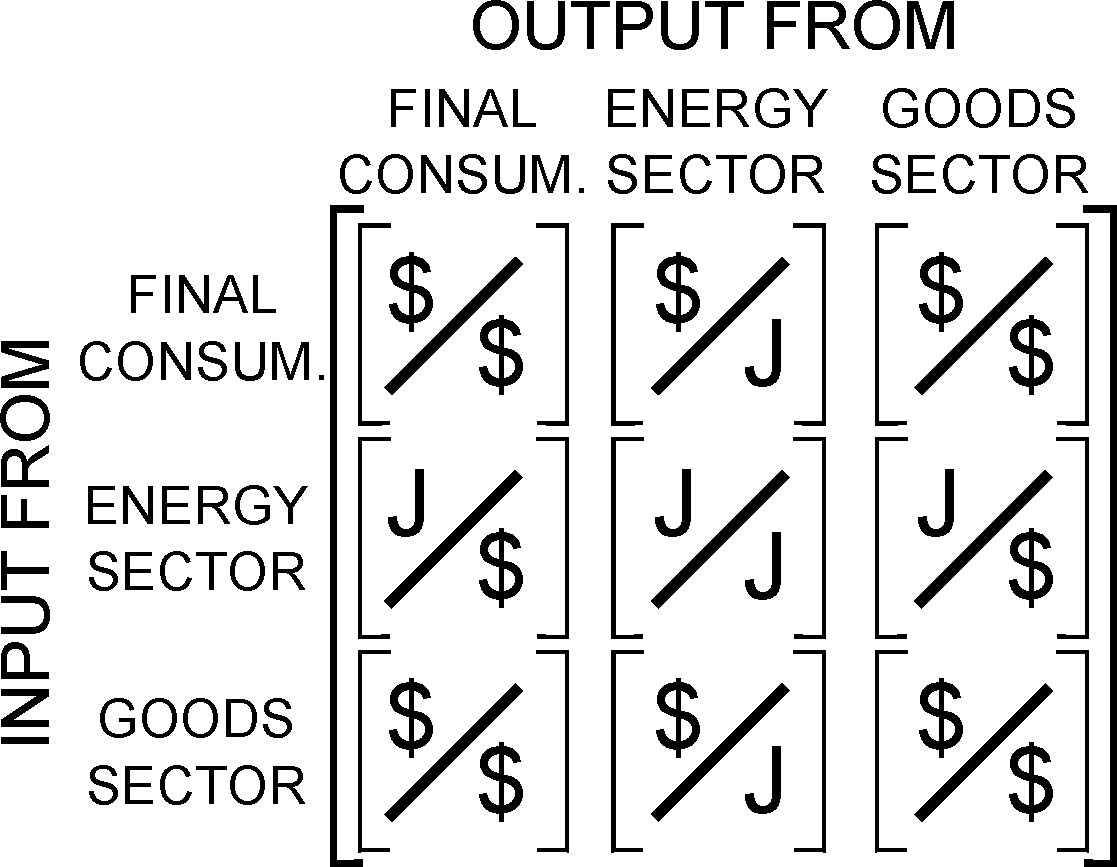
\includegraphics[width=0.4\linewidth]{Part_2/Chapter_Intensity/images/I-O_units.pdf}
\caption[Units for input-output ratios]{ Units for input-output ratios ($a$).}
\label{fig:A_matrix_units}
\end{figure}

Equations~\ref{eq:epsilon_transfers_1}, 
\ref{eq:epsilon_equiv_1}, and 
\ref{eq:aij_def} can be combined to give

\begin{equation}
	\dot{T}_{jk} = \varepsilon_{j} a_{jk} \dot{X}_{k}.
\end{equation}


%%%%%%%%%% Example A %%%%%%%%%%
\section{Example A: single-sector economy} % chktex 13
%%%%%%%%%%

With reference to Figures~\ref{fig:A_energy}, 
\ref{fig:A_total_energy_T_dot}, 
and~\ref{fig:A_value},
the energy intensity ($\varepsilon_{1}$) of a single-sector economy is calculated by

\begin{equation} \label{eq:A-energy_intensity}
	\varepsilon_{1} 
	= \frac{\dot{T}_{1}}{\dot{X}_{1}} 
	= \frac{\dot{T}_{11}}{\dot{X}_{11}}.
\end{equation}

Appendix~\ref{chap:infinite_series} illustrates that the energy 
intensity of a single-sector economy ($\varepsilon_{1}$) 
is comprised of the sum of the infinite recursions
of energy consumed during production of output ($\dot{X}_{1}$).

To estimate energy intensities
when more than one economic sector is involved, 
we move to Examples~B and~C in the following sections.


%%%%%%%%%% Example B %%%%%%%%%%
\section{Example B: two-sector economy} % chktex 13
%%%%%%%%%%

With reference to Figures~\ref{fig:B_energy}, 
\ref{fig:B_total_energy},
and~\ref{fig:B_value}, 
the energy intensity ($\varepsilon_{2}$) 
of the production sector is given by

\begin{equation} \label{eq:single_sector_energy_intensity}
	\varepsilon_{2} 
	= \frac{\dot{T}_{2}}{\dot{X}_{2}} 
	= \frac{\dot{T}_{22}}{\dot{X}_{22}}.
\end{equation}

\noindent{}Thus,

\begin{equation} \label{eq:T_dot_1_single_sector}
	\dot{T}_{2} = \varepsilon_{2}\dot{X}_{2},
\end{equation}

The input-output ratio 
for the production sector's self-use of output ($a_{22}$) is

\begin{equation} \label{eq:io_ratio_single_sector}
	a_{22} = \frac{\dot{X}_{22}}{\dot{X}_{2}},
\end{equation}

\noindent{}thus

\begin{equation} \label{eq:T_dot_11_single_sector}
	\dot{T}_{22} = \varepsilon_{2}a_{22}\dot{X}_{2}.
\end{equation}

We can rewrite the total energy accounting equation 
for the two-sector economy

\begin{equation}
	\frac{\mathrm{d}T_{2}}{\mathrm{d}t} 	 
	= \dot{T}_{02} 
	+ \dot{T}_{12}
	+ \dot{T}_{22} 
	- \dot{T}_{2} 
	- \dot{T}_{20} \tag{\ref{eq:CV_T_2}}
\end{equation}

\noindent{}using energy intensity by realizing that 

\begin{itemize}
	\item{$\frac{\mathrm{d}E_2}{\mathrm{d}t} = 0$
		and
		$\frac{\mathrm{d}T_2}{\mathrm{d}t} = \frac{\mathrm{d}B_2}{\mathrm{d}t}$, 
		because direct energy
		does not accumulate within economic sectors,}
	\item{$\frac{\mathrm{d}B_2}{\mathrm{d}t} = \frac{\mathrm{d}B_{K_{2}}}{\mathrm{d}t}$,
		because resources ($R$) and short-lived materials ($S$) do not 
		accumulate at appreciable rates in economic sectors,}
	\item{$\dot{B}_{02} = 0$ and $\dot{T}_{02} = \dot{E}_{02}$,
		because embodied energy appears only in the \emph{output} of a sector,}
	\item{$\dot{E}_{20} = 0$ and $\dot{T}_{20} = \dot{B}_{20}$, 
	because direct energy is not wasted to the biosphere at any significant rate, and} 
	\item{$\dot{B}_{20} = \left( \dot{B}_{\dot{R}_{20}} 
							+ \dot{B}_{\dot{S}_{20}}
							+ \dot{B}_{\dot{K}_{20}}
							\right)
						= \left( \dot{B}_{\dot{R}_{20}} 
							+ \dot{B}_{\dot{S}_{20}}
							+ \gamma_{B,2} B_{K_{2}}
							\right)$, as shown in Section~\ref{sec:Embodied_Energy_Example_C}.}
\end{itemize}

\noindent{}If we substitute Equations~\ref{eq:T_dot_1_single_sector} 
and~\ref{eq:T_dot_11_single_sector} into Equation~\ref{eq:CV_T_2}, we obtain

\begin{equation} \label{eq:dB1/dt_single_sector_after_substituting_eps_and_a}
	\frac{\mathrm{d}B_{K_{2}}}{\mathrm{d}t} 
	= \dot{E}_{02} 
	+ \dot{T}_{12}
	+ \varepsilon_{2}a_{22}\dot{X}_{2} 
	- \varepsilon_{2}\dot{X}_{2} 
	- \left( \dot{B}_{\dot{R}_{20}} 
							+ \dot{B}_{\dot{S}_{20}}
							+ \gamma_{B,2} B_{K_{2}}
							\right).
\end{equation}

Equation~\ref{eq:dB1/dt_single_sector_after_substituting_eps_and_a}
can be solved for energy intensity ($\varepsilon_{2}$) to obtain

\begin{equation} \label{eq:B-epsilon}
	\varepsilon_{2}
	= {(1 - a_{22})}^{-1} {\dot{X}_{2}}^{-1} 
		\left[
			\dot{E}_{02}
			+ \dot{T}_{12}
			- \frac{\mathrm{d}B_{K_{2}}}{\mathrm{d}t} 
			- \dot{B}_{\dot{R}_{20}}
			- \dot{B}_{\dot{S}_{20}}
			- \gamma_{B,2} B_{B_{2}}
		\right]
\end{equation}

To extend Equation~\ref{eq:B-epsilon}
to a matrix formulation, we turn to Example~C.


%%%%%%%%%% Example C %%%%%%%%%%
\section{Example~C: three-sector economy} % chktex 13
\label{sec:C-intensity}
%%%%%%%%%%

The three-sector economy of Example~C affords the opportunity 
to develop a matrix version 
of the total energy accounting equation (\ref{eq:C-CV_T_123})
and to develop an equation that estimates the
energy intensity of economic sectors. 
We begin with a matrix version of the total energy accounting equation.


%+++++++++ Example C: Total energy equation ++++++++++
\subsection{Total energy accounting equation}
%+++++++++

We apply Equation~\ref{eq:C-CV_T_123} to the three-sector
economy shown in 
Figures~\ref{fig:C_energy},~\ref{fig:C_total_energy}, and~\ref{fig:C_value}
to obtain the following total energy accounting equations
for the Energy~(2) and Goods and Services~(3) sectors 
of the three-sector economy:

\begin{equation} \label{eq:C-Total_Energy_Sec_2-a}
	\frac{\mathrm{d}T_{2}}{\mathrm{d}t} 
	= \dot{T}_{02}  
	+ \dot{T}_{12}
	+ \dot{T}_{22}
	+ \dot{T}_{32}
	- \dot{T}_{2}
	- \dot{T}_{20}
\end{equation}

\noindent{}and

\begin{equation} \label{eq:C-Total_Energy_Sec_3-a}
	\frac{\mathrm{d}T_{3}}{\mathrm{d}t} 
	= \dot{T}_{03}  
	+ \dot{T}_{13}
	+ \dot{T}_{23}
	+ \dot{T}_{33}
	- \dot{T}_{3}
	- \dot{T}_{30}.
\end{equation}

\noindent{}Similar to Example~B, we realize that 

\begin{itemize}
	\item{$\frac{\mathrm{d}E_i}{\mathrm{d}t} = 0$
		and
		$\frac{\mathrm{d}T_i}{\mathrm{d}t} = \frac{\mathrm{d}B_i}{\mathrm{d}t}$, 
		because direct energy
		does not accumulate within economic sectors,}
	\item{$\frac{\mathrm{d}B_i}{\mathrm{d}t} = \frac{\mathrm{d}B_{K_{i}}}{\mathrm{d}t}$,
		because resources ($R$) and short-lived materials ($S$) do not 
		accumulate at appreciable rates in economic sectors,}
	\item{$\dot{B}_{0j} = 0$ and $\dot{T}_{0j} = \dot{E}_{0j}$,
		because embodied energy appears only in the \emph{output} of a sector,}
	\item{$\dot{E}_{j0} = 0$ and $\dot{T}_{j0} = \dot{B}_{j0}$, 
	because direct energy is not wasted to the biosphere at any significant rate, and} 
	\item{$\dot{B}_{j0} = \left( \dot{B}_{\dot{R}_{j0}} 
							+ \dot{B}_{\dot{S}_{j0}}
							+ \dot{B}_{\dot{K}_{j0}}
							\right)
						= \left( \dot{B}_{\dot{R}_{j0}} 
							+ \dot{B}_{\dot{S}_{j0}}
							+ \gamma_{B,j} B_{K_{j}}
							\right)$, as shown in Section~\ref{sec:Embodied_Energy_Example_C}.}
\end{itemize}

\noindent{}to obtain

\begin{equation} \label{eq:C-Total_Energy_Sec_2-b}
	\frac{\mathrm{d}B_{K_{2}}}{\mathrm{d}t}
	= \dot{E}_{02}
	+ \dot{T}_{12}
	+ \varepsilon_{2} \dot{X}_{22}
	+ \varepsilon_{3} \dot{X}_{32}
	- \varepsilon_{2} \dot{X}_{2}
	- \left( \dot{B}_{\dot{R}_{20}} 
							+ \dot{B}_{\dot{S}_{20}}
							+ \gamma_{B,2} B_{K_{2}}
							\right)
\end{equation}

\noindent{}and

\begin{equation} \label{eq:C-Total_Energy_Sec_3-b}
	\frac{\mathrm{d}B_{K_{3}}}{\mathrm{d}t}
	= \dot{E}_{03}
	+ \dot{T}_{13}
	+ \varepsilon_{2} \dot{X}_{23}
	+ \varepsilon_{3} \dot{X}_{33}
	- \varepsilon_{3} \dot{X}_{3}
	- \left( \dot{B}_{\dot{R}_{30}} 
							+ \dot{B}_{\dot{S}_{30}}
							+ \gamma_{B,3} B_{K_{3}}
							\right).
\end{equation}


%%%%%%%%%% Example C: Matrix formulation %%%%%%%%%%
\subsection{Matrix formulation} % chktex 13
\label{sec:C-matrix}
%%%%%%%%%%

Equations~\ref{eq:C-Total_Energy_Sec_2-b} 
and~\ref{eq:C-Total_Energy_Sec_3-b} can be rewritten 
in vector notation as

\begin{equation} \label{eq:C-Expanded_Matrix_Form}
	\begin{split}
		\begin{Bmatrix}
			\frac{\mathrm{d}B_{K_{2}}}{\mathrm{d}t} \\[0.4em] % Adds some vertical space.
			\frac{\mathrm{d}B_{K_{3}}}{\mathrm{d}t} 
		\end{Bmatrix}
		=
		\begin{Bmatrix}
			\dot{E}_{02}\\
			\dot{E}_{03}
		\end{Bmatrix}
		& +                                               % & sets alighment tab
		\begin{Bmatrix}
			\dot{T}_{12}\\
			\dot{T}_{13}
		\end{Bmatrix}
		+
		\begin{bmatrix}
			\dot{X}_{22} & \dot{X}_{32}\\
			\dot{X}_{23} & \dot{X}_{33}
		\end{bmatrix}
		\begin{Bmatrix}
			\varepsilon_{2}\\
			\varepsilon_{3}
		\end{Bmatrix}   
		- 
		\begin{bmatrix}
			\dot{X}_{2} & 0          \\
			0           & \dot{X}_{3}
		\end{bmatrix}
		\begin{Bmatrix}
			\varepsilon_{2}\\
			\varepsilon_{3}
		\end{Bmatrix} \\                                 % \\ gives line break
		& -                                              % & aligns to previous tab
		\begin{Bmatrix}
			\dot{B}_{\dot{R}_{20}}  \\
			\dot{B}_{\dot{R}_{30}} 
		\end{Bmatrix}
		-
		\begin{Bmatrix}
			\dot{B}_{\dot{S}_{20}}  \\
			\dot{B}_{\dot{S}_{30}} 
		\end{Bmatrix}
		-
		\begin{bmatrix}
			\gamma_{B,2} & 0          \\
			0            & \gamma_{B,3}
		\end{bmatrix}
		\begin{Bmatrix}
			B_{K_{2}}\\
			B_{K_{3}}
		\end{Bmatrix}.
	\end{split}
\end{equation}

\noindent{}If we define the following matrices and vectors:

\begin{equation} \label{eq:B_vec_def}
	\vec{B}_{K} 
	\equiv
	\begin{Bmatrix}	
		B_{K_{2}} \\
		B_{K_{3}}
	\end{Bmatrix},
\end{equation}

\begin{equation} \label{eq:dBdt_vec_def}
	\frac{\mathrm{d}\vec{B}_K}{\mathrm{d}t} 
	\equiv
	\begin{Bmatrix}	
		\frac{\mathrm{d}B_{K_{2}}}{\mathrm{d}t}	\\[0.4em] % Adds some vertical space.
		\frac{\mathrm{d}B_{K_{3}}}{\mathrm{d}t}
	\end{Bmatrix},
\end{equation}

\begin{equation} \label{eq:E_vec_def}
	\vec{E}_{0} 
	\equiv
	\begin{Bmatrix}
		\dot{E}_{02} \\
		\dot{E}_{03}
	\end{Bmatrix},
\end{equation} \nomenclature[E]{$\vec{E}_{0}$}{vector of direct energy inputs 
												from the biosphere [W]}

\begin{equation} \label{eq:T_vec_def}
	\vec{T}_{1} 
	\equiv
	\begin{Bmatrix}
		\dot{T}_{12} \\
		\dot{T}_{13}
	\end{Bmatrix},
\end{equation} \nomenclature[T]{$\vec{T}_{1}$}{vector of total energy inputs 
												from society to the economy [W]}

\begin{equation} \label{eq:X_t_matrix_def}
	\vec{X}_{t} 
	\equiv
	\begin{bmatrix}
		\dot{X}_{22} & \dot{X}_{23} \\
		\dot{X}_{32} & \dot{X}_{33}
	\end{bmatrix},
\end{equation} \nomenclature[X]{$\vec{X}_{t}$}{transaction matrix [\$/year]}
\index{transaction matrix}\index{matrix!transaction|see{transaction matrix}}

\begin{equation} \label{eq:eps_vec_def}
	\bm{\varepsilon} 
	\equiv
	\begin{Bmatrix}
		\varepsilon_{2}	\\
		\varepsilon_{3}
	\end{Bmatrix},
\end{equation} \nomenclature[e]{$\bm{\varepsilon}$}{column vector 
								of sector energy intensities [J/\$]}
								
\begin{equation} \label{eq:waste_vec_def}
	\vec{B}_{waste} 
	=
	\begin{Bmatrix}
		\dot{B}_{waste,{20}}	\\
		\dot{B}_{waste,{30}}	\\
	\end{Bmatrix}
	\equiv
	\begin{Bmatrix}
		\dot{B}_{\dot{R}_{20}}	\\
		\dot{B}_{\dot{R}_{30}}	\\
	\end{Bmatrix}
	+
	\begin{Bmatrix}
		\dot{B}_{\dot{S}_{20}}	\\
		\dot{B}_{\dot{B}_{30}}	\\
	\end{Bmatrix},
\end{equation} \nomenclature[B]{$\vec{B}_{waste}$}{column vector 
								of waste embodied energy from resource ($\dot{R}$)
								and short-lived material ($\dot{S}$) flow [J/s]}

\begin{equation} \label{eq:X_hat_matrix_def}
	\hat{\vec{X}} 
	\equiv
	\delta_{ij} \dot{X}_{j} 
	= 
	\begin{bmatrix}
		\dot{X}_{2}		&	0	  \\
		0				&	\dot{X}_{3}	\\
	\end{bmatrix},
\end{equation} \nomenclature[X]{$\hat{\vec{X}}$}{matrix of sector outputs [\$/year]}

\noindent{}and

\begin{equation} \label{eq:gamma_hat_matrix_def}
	\hat{\bm{\gamma}}_{B}
	\equiv
	\delta_{ij} \gamma_{B,j}
	=
	\begin{bmatrix}
		\gamma_{B,2} & 0         \\
		0            & \gamma_{B,3}
	\end{bmatrix};
\end{equation}\nomenclature[g]{$\hat{\bm{\gamma}}$}{diagonal matrix of depreciation rates [\$/year]}

\noindent{}with the ``Kronecker delta''

\begin{equation}\label{eq:k_delta}
	\delta_{ij} 
	\equiv
	\begin{cases}	
		0	&	\text{if  } i \neq j	\\
		1 	& 	\text{if  } i = j
	\end{cases};
\end{equation}\nomenclature[d]{$\delta_{ij}$}{Kronecker delta}

\noindent{}we can rewrite Equation~\ref{eq:C-Expanded_Matrix_Form}
compactly as

\begin{equation} \label{eq:matrix_leontief_pre_1}
	\frac{\mathrm{d}\vec{B}_{K}}{\mathrm{d}t} 
	= \vec{E}_{0}
	+ \vec{T}_{1}
	+ \vec{X}_{t}^{\mathrm{T}}\bm{\varepsilon} 
	- \hat{\vec{X}}\bm{\varepsilon}
	- \vec{B}_{waste}
	- \hat{\bm{\gamma}}_{B} \vec{B}_{K}.
\end{equation}

\noindent{}Equation~\ref{eq:matrix_leontief_pre_1} can be simplified to

\begin{equation} \label{eq:matrix_leontief_pre_2}
	\frac{\mathrm{d}\vec{B}_{K}}{\mathrm{d}t} 
	= \vec{E}_{0}
	+ \vec{T}_{1}
	+ (\vec{X}_{t}^{\mathrm{T}} - \hat{\vec{X}})\bm{\varepsilon} 
	- \vec{B}_{waste}
	- \hat{\bm{\gamma}}_{B}\vec{B}_{K}.
\end{equation}

\noindent{}We can define the input-output matrix ($\vec{A}$) as

\begin{equation} \label{eq:A_matrix_def}
	\vec{A} 
	\equiv
	\begin{bmatrix}
		a_{22} & a_{23}	\\
		a_{32} & a_{33}	
	\end{bmatrix}.
\end{equation} \nomenclature[A]{$\vec{A}$}{input-output matrix [-]}
\index{input-output matrix}\index{matrix!input-output|see{input-output matrix}}

\noindent{}Appendix~\ref{app:Proof} shows that

\begin{equation} \label{eq:Xdifference1}
	\vec{X}_{t}^{\mathrm{T}} 
	- \hat{\vec{X}} 
	= \hat{\vec{X}} (\vec{A}^{\mathrm{T}} - \vec{I}),
\end{equation}

\noindent{}which allows Equation~\ref{eq:matrix_leontief_pre_2}
to be recast as

\begin{equation} \label{eq:matrix_leontief}
	\frac{\mathrm{d}\vec{B}_{K}}{\mathrm{d}t} 
	= \vec{E}_{0}
	+ \vec{T}_{1}
	+ \hat{\vec{X}} (\vec{A}^{\mathrm{T}} - \vec{I})\bm{\varepsilon} 
	- \vec{B}_{waste}
	- \hat{\bm{\gamma}}_{B}\vec{B}_{K}.
\end{equation}

\noindent{}Equation~\ref{eq:matrix_leontief} is the matrix version 
of the total energy accounting equation
written in terms of embodied energy ($\vec{B}$), 
energy intensities ($\bm{\varepsilon}$),
and input-output ratios ($\vec{A}$).
Equation~\ref{eq:C-Expanded_Matrix_Form} applies 
for the three-sector economy of Example~C, 
but the equivalent matrix formulation (Equation~\ref{eq:matrix_leontief}) 
can be extended to any desired level 
of economic and energy sector disaggregation 
by expanding the vectors and matrices in 
Equations~\ref{eq:dBdt_vec_def}--\ref{eq:B_vec_def}
and~\ref{eq:A_matrix_def} to include
all sectors of the economy.\cite{Bullard:1978vd,Casler1984}

Equation~\ref{eq:matrix_leontief} provides a means to 
estimate the embodied energy accumulation rate
in economic sectors $\left(\frac{\mathrm{d}\vec{B}_{K}}{\mathrm{d}t}\right)$ 
knowing only 
direct energy inputs to the economy from the biosphere ($\vec{E}_{0}$), 
total energy inputs from society to the economy ($\vec{T}_{1}$),
sector outputs ($\hat{\vec{X}}$), 
sector input-output ratios ($\vec{A}$), 
sector energy intensities ($\bm{\varepsilon}$), 
energy embodied in wastes from the economy ($\vec{B}_{waste}$),
and physical depreciation rates of capital stock ($\hat{\bm{\gamma}}_{B}\vec{B}_{K}$). 
In theory, the transaction matrix ($\vec{X}_{t}$) is not required 
if the input-ouput matrix ($\vec{A}$) is known, 
though in practice, 
knowledge of input-output matrix ($\vec{A}$) 
would be derived from the transaction matrix ($\vec{X}_{t}$),
as shown in Appendix~\ref{chap:Estimating_A}.


% %%%%%%%%%% Example C %%%%%%%%%%
% \section{Estimating $\bm{\varepsilon}$}
% \label{sec:estimating_epsilon-intensity_chapter}
% %%%%%%%%%%

Equation~\ref{eq:matrix_leontief} can be rearranged to obtain

\begin{equation} \label{eq:epsilon_derivation_1}
	\hat{\vec{X}} (\vec{A}^{\mathrm{T}} - \vec{I}) \bm{\epsilon}
	= \frac{\mathrm{d}\vec{B}_{K}}{\mathrm{d}t}
	+ \vec{B}_{waste}
	+ \hat{\bm{\gamma}}_{B} \vec{B}_{K}
	- \vec{E}_{0}
	- \vec{T}_{1} 
\end{equation}

\noindent{}and

\begin{equation} \label{eq:epsilon_derivation_2}
	\bm{\epsilon}
	= {\left[ \hat{\vec{X}} (\vec{A}^{\mathrm{T}} - \vec{I}) \right]}^{-1}
		\left[
			\frac{\mathrm{d}\vec{B}_{K}}{\mathrm{d}t}
			+ \vec{B}_{waste}
			+ \hat{\bm{\gamma}}_{B} \vec{B}_{K}
			- \vec{E}_{0}
			- \vec{T}_{1} 
		\right].
\end{equation}

\noindent{}We apply the matrix identity 
from Formula 6.2, p. 308 in Beyer~\cite{Beyer:1991vd}

\begin{equation} \label{eq:matrix_identity_Beyer}
	{\left(\vec{A}\vec{B}\vec{C}\right)}^{-1} 
	= \vec{C}^{-1} \vec{B}^{-1} \vec{A}^{-1}
\end{equation}

\noindent{}to the right side of Equation~\ref{eq:epsilon_derivation_2} to obtain

\begin{equation} \label{eq:epsilon_derivation_3}
	\bm{\epsilon}
	= {(\vec{A}^{\mathrm{T}} - \vec{I})}^{-1} {\hat{\vec{X}}}^{-1} 
		\left[
			\frac{\mathrm{d}\vec{B}_{K}}{\mathrm{d}t}
			+ \vec{B}_{waste}
			+ \hat{\bm{\gamma}}_{B} \vec{B}_{K}
			- \vec{E}_{0}
			- \vec{T}_{1} 
		\right].
\end{equation}

\noindent{}Finally, we can multiply both parenthetical terms\footnote{The parenthetical
terms on the right side of Equation~\ref{eq:epsilon_derivation_3} 
are $(\vec{A}^{\mathrm{T}} - \vec{I})$ and
$
\left[
	\frac{\mathrm{d}\vec{B}_{K}}{\mathrm{d}t}
	+ \vec{B}_{waste}
	+ \hat{\bm{\gamma}}_{B} \vec{B}_{K}
	- \vec{E}_{0}
	- \vec{T}_{1} 
\right]
$.} 
on the right side of Equation~\ref{eq:epsilon_derivation_3} by $-1$ to obtain

\begin{equation} \label{eq:epsilon_leontief_with_A}
	\bm{\varepsilon} 
	= {(\vec{I} - \vec{A}^{\mathrm{T}})}^{-1}\hat{\vec{X}}^{-1}
		\left[\vec{E}_{0} 
				+ \vec{T}_{1} 
				- \frac{\mathrm{d}\vec{B}_{K}}{\mathrm{d}t} 
				- \vec{B}_{waste}
				- \hat{\bm{\gamma}}_{B}\vec{B}_{K}
		\right].
\end{equation}

Equation~\ref{eq:epsilon_leontief_with_A} provides a means 
to estimate energy intensity ($\bm{\varepsilon}$)
of the sectors of the economy. 
But, the effect of physical depreciation of capital stock
($\hat{\bm{\gamma}}_{B}\vec{B}_{K}$) 
can be clarified.
We do so in the following section.

%%%%%%%%%% Example C %%%%%%%%%%
\section{The effect of capital flows}
\label{sec:intensity_capital_correction}
%%%%%%%%%%

*********** Folding this content into the
Implications section on the I-O method. 
Delete this section after completing the Implications section
on the I-O method. ************

From Equation~\ref{eq:epsilon_leontief_with_A},
it is clear that flows of capital stock affect
the embodied energy of products.
Unfortunately, flows of capital stock ($\dot{K}$) are not logged in the 
Bureau of Economic Analysis (BEA) standard I-O tables.\footnote{See
Section~\ref{sec:Data} for a discussion of data needs.}
Historically, only a few energy analysts attempted to include the effect
of capital flows on energy intensity ($\bm{\varepsilon}$). 
Bullard~\cite{Bullard1975} added capital stock purchases as an input
to each economic sector.
Casler~\cite{Casler:1983uy} attempted to correct the BEA's
input-output tables prior to applying the I-O method.
However, the present analysis affords the opportunity
to develop a mathematically-rigorous approach to the 
effects of physical depreciation based on 
the model of material, energy, and value flows presented 
in Chapters~\ref{chap:materials}--\ref{chap:value}.

Our approach derives




Physical depreciation\index{depreciation!physical} 
of capital stock ($\hat{\bm{\gamma}}_{K}\vec{B}_{K}$)
occurs due to wear and tear, obsolescence, and end-of-life
of material and capital stock\index{capital stock} 
within economic sectors and society.\footnote{Physical depreciation
is different from financial depreciation. 
Financial depreciation occurs during the useful life of material, 
while physical depreciation occurs at end of life, 
when material is discarded from an economic sector to the biosphere.}
But, we note that depreciation ($\hat{\bm{\gamma}}_{K} \vec{B}_{K}$) 
and accumulation of embodied energy 
$\left( \frac{\mathrm{d}\vec{B}_{K}}{\mathrm{d}t} \right)$
should be considered in tandem,
because the outflow of embodied energy due to depreciation
($\hat{\bm{\gamma}}_{K} \vec{B}_{K}$)
will cause an equal reduction of the net accumulation rate of embodied energy
$\left( \frac{\mathrm{d}\vec{B}_{K}}{\mathrm{d}t} \right)$
within economic sectors.

We can split the embodied energy accumulation rate 
$\left( \frac{\mathrm{d}\vec{B}_{K}}{\mathrm{d}t} \right)$
into a portion due to depreciation and a portion due to 
factors such as growth that are exclusive of physical depreciation as follows:

\begin{equation} \label{eq:dB_dt_split}
	\frac{\mathrm{d}\vec{B}_{K}}{\mathrm{d}t} 
	= \left. \frac{\mathrm{d}\vec{B}_{K}}{\mathrm{d}t} \right|_{\mathrm{other}} 
	+ \left. \frac{\mathrm{d}\vec{B}_{K}}{\mathrm{d}t} \right|_{\mathrm{depreciation}}.
\end{equation}

\noindent{}When physical depreciation occurs,
$\gamma_{K,i} B_{K_{i}} > 0$ and 
$\left. \frac{\mathrm{d}B_{K_{i}}}{\mathrm{d}t} \right|_{\mathrm{depreciation}} < 0$.
To be specific,

\begin{equation} \label{eq:dB_dt_dep_equals_dep}
	\left. \frac{\mathrm{d}B_{K_{i}}}{\mathrm{d}t} \right|_{\mathrm{depreciation}} 
	+ \gamma_{K,i} B_{K_{i}}
	= 0.
\end{equation}

\noindent{}Substituting Equations~\ref{eq:dB_dt_split} and~\ref{eq:dB_dt_dep_equals_dep}
into Equation~\ref{eq:epsilon_leontief_with_A} and extending to matrix notation yields

\begin{equation} \label{eq:epsilon_leontief_depreciation_simplification}
	\bm{\varepsilon} 
	= {(\vec{I} - \vec{A}^{\mathrm{T}})}^{-1}\hat{\vec{X}}^{-1}
		\left[\vec{E}_{0} 
				+ \vec{T}_{1} 
				- \left. \frac{\mathrm{d}\vec{B}_{K}}{\mathrm{d}t} \right|_{\mathrm{other}}
				- \vec{B}_{waste}
		\right].
\end{equation}

\noindent{}Equation~\ref{eq:epsilon_leontief_depreciation_simplification} 
allows estimation of the energy intensity 
of economic output ($\bm{\varepsilon}$) 
knowing only 
sector input-output ratios ($\vec{A}$), 
sector outputs ($\hat{\vec{X}}$), 
energy input to the economy from the biosphere~($\vec{E}_{0}$), 
total energy input from society to the economy~($\vec{T}_{1}$),
sector embodied energy accumulation rates
exclusive of the effects of physical
depreciation~$\left( \left. \frac{\mathrm{d}\vec{B}_{K}}{\mathrm{d}t} \right|_{\mathrm{other}} \right)$,
and the waste rate of embodied energy due to scrapped resources and short-lived material flows
($\vec{B}_{waste}$).
Again, the transaction matrix\index{transaction matriux} ($\vec{X}_{t}$) 
is not required for estimating the energy intensity 
of economic sectors ($\bm{\varepsilon}$)
if the input-ouput matrix ($\vec{A}$) is known, 
though in practice, 
knowledge of input-output matrix ($\vec{A}$) 
would be derived from the transaction matrix ($\vec{X}_{t}$),
as shown in Appendix~\ref{chap:Estimating_A}.

Table~\ref{tab:embodied_energy_accumulation_factors} 
describes the importance of each term in 
Equation~\ref{eq:epsilon_leontief_depreciation_simplification}.\footnote{In
Table~\ref{tab:embodied_energy_accumulation_factors}, the term ``energy'' can be 
taken to include both direct ($\dot{E}$) and embodied ($\dot{B}$) energy.
Also, values in $\vec{A}$ are less than unity 
and the term $(\vec{I} - \vec{A})$ 
in Equation~\ref{eq:epsilon_leontief_depreciation_simplification} 
is inverted. 
Thus, as values in $\vec{A}$ increase, 
the term $(\vec{I} - \vec{A})$ in the ``denominator'' decreases, 
and $\varepsilon$ increases.} 

\begin{table}
\caption[Factors affecting the energy intensity of economic output.]{Factors from
Equation~\ref{eq:epsilon_leontief_depreciation_simplification} 
affecting the energy intensity of economic output ($\vec{\bm{\varepsilon}}$).}
\begin{center}
  \begin{tabular}{r @{\hspace{2em}} l}
	  
    \toprule
	
    Factor & Implication \\ 
	
	\midrule
    
	$\vec{A}$ & As $\vec{A}$$\uparrow$, more energy 
	flows into sectors per unit output, 
	and $\bm{\varepsilon}$$\uparrow$.\\
	
	$\hat{\vec{X}}$ & As $\hat{\vec{X}}$$\uparrow$, economic output increases, 
	and $\bm{\varepsilon}$$\downarrow$.  \\
	
	$\vec{E}_{0}$ & As $\vec{E}_{0}$$\uparrow$, 
	the rate of energy flow from the biosphere increases, 
	and $\bm{\varepsilon}$$\uparrow$.  \\ 
	
	$\vec{T}_{1}$ & As $\vec{T}_{1}$$\uparrow$, 
	the flow of useful work to the economy increases, 
	and $\bm{\varepsilon}$$\uparrow$.  \\ 
	
	$\left. \frac{\mathrm{d}\vec{B}_{K}}{\mathrm{d}t} \right|_{\mathrm{other}}$ & 
	As $\left. \frac{\mathrm{d}\vec{B}_{K}}{\mathrm{d}t} \right|_{\mathrm{other}}$$\uparrow$, 
	inflowing energy goes into capital instead of products, 
	and $\bm{\varepsilon}$$\downarrow$. \\
	
	$\vec{B}_{waste}$ & As $\vec{B}_{waste}$$\uparrow$, 
	energy is wasted rather than embodied in products,
	and $\bm{\varepsilon}$$\downarrow$. \\

	\bottomrule
	
  \end{tabular}
\end{center}
\label{tab:embodied_energy_accumulation_factors}
\end{table}





Equation~\ref{eq:epsilon_leontief_depreciation_simplification}
is an important result that is directly comparable with the I-O literature,
and we will do so in Chapter~\ref{chap:implications}.
But first, the following section examines energy intensity 
in the context of our running example, the auto industry.

%%%%%%%%%% Intensity: Auto industry example %%%%%%%%%%
\section{Energy intensity of the US auto industry}
\label{sec:intensity_auto}
%%%%%%%%%%

Equation~\ref{eq:epsilon_leontief_depreciation_simplification} shows 
that it is possible to estimate the energy intensity 
of products of economic sectors using the Input-Output method.\footnote{For a discussion
of differences between Equation~\ref{eq:epsilon_leontief_depreciation_simplification} 
and similar equations in the literature, 
see Appendix~\ref{chap:Casler}.}
Several studies have used similar energy-based, 
input-output methods to estimate the energetic
cost of goods and services produced by various
economic sectors.\cite{Bullard1975, Costanza:1980ww, Costanza:1984tq, EIOLCA2014, Hendrickson2006,
Herendeen1973, Herendeen1974, Herendeen1974a, Herendeen1978,
Wright1974, Lenzen1998, Machado2001}
We review a few of these studies below.

**** MCD---do we know of a way to make these references
appear as [1--10]? biblatex is not compatible with chapterbib. ****

Using national accounts data for 1967,
Bullard and Herendeen calculated the
total energy consumption rate~($\dot{T}$)
of the US automobile industry as 
$13,240 \times 10^{15}$~joules/year~$= 13.24$~EJ,
which was around 20\% of the nation's
energy consumption in that year.\cite{Bullard1975}
Around half of this energy was directly
consumed within the auto industry itself~($\dot{Q}_{j0}$),
meaning the rest was upstream consumption
in material processing, 
entering the auto industry as embodied 
energy~($\sum_{i}\dot{B}_{ij}$).
Given the number of autos produced per year, 
Bullard and Herendeen calculated that 
the embodied energy per vehicle was 148 GJ (10$^{9}$~J),
11\% higher than the estimate obtained via process analysis in a
study by Berry and Fels~\cite{Berry:1973vo} two years earlier.\footnote{See
Section~\ref{sec:embodied_energy_auto} for discussion 
of the Berry and Fels~\cite{Berry:1973vo} paper.}

In 1980, Costanza~\cite{Costanza:1980ww} estimated 
the energy intensity of all economic sectors of the US economy
using the Input-Output method.
Unfortunately, the energy intensity 
of the Motor Vehicles and Equipment sector (63) was not reported
in~\cite{Costanza:1980ww}.
Later, Costanza and Herendeen~\cite{Costanza:1984tq} re-estimated
energy intensity and reported the energy intensity 
of outputs from all 87 Bureau of Economic Affairs\index{Bureau of Economic Affairs} 
(BEA) sectors.
The energy intensity of the Motor Vehicles and Equipment sector (63) 
and selected other sectors are given in 
Tables~\ref{tab:C_and_H_auto_energy_intensities}
and~\ref{tab:C_and_H_selected_energy_intensities}.\footnote{Values 
from Costanza and Herendeen's 
DIRECT method are provided here. 
See Section~\ref{sec:energy_input_vector} for discussion
of the differences between DIRECT and DEC methods
and justification for reporting
DIRECT method values only.} 

\begin{table}
\caption{Motor Vehicles and Equipment sector (63) 
		energy intensity values.\cite{Costanza:1984tq}}
\begin{center}
\begin{tabular} {r @{\hspace{2em}} l}
	\toprule
	Year & Energy Intensity [kJ/\$] \\
	\midrule
	1963 & $1.16\times10^{5}$ \\
	1967 & $1.04\times10^{5}$ \\
	1972 & $0.95\times10^{5}$ \\
	\bottomrule
\end{tabular}
\end{center}
\label{tab:C_and_H_auto_energy_intensities}
\end{table}

\begin{table}
\caption{Selected US economic sector energy intensities, 1972.\cite{Costanza:1984tq}}
\begin{center}
\begin{tabular} {r @{\hspace{2em}} l}
	\toprule
	Sector &  Energy Intensity [kJ/\$] \\
	\midrule
	Coal Mining (1)                   & $3.23\times10^{6}$ \\
	Air Transport (73)                & $1.76\times10^{5}$ \\
	New Construction (14)             & $1.03\times10^{5}$ \\
	Motor Vehicles and Equipment (63) & $9.50\times10^{4}$ \\
	Auto Repair (82)                  & $8.35\times10^{4}$ \\
	\bottomrule
\end{tabular}
\end{center}
\label{tab:C_and_H_selected_energy_intensities}
\end{table}

However, the Costanza results~\cite{Costanza:1984tq} 
(and nearly all I-O results in the literature)
assume the following: negligible energy input from society 
(which is probably a reasonable assumption for the US), 
steady-state economic conditions with negligible accumulation 
of embodied energy in economic sectors 
(which probably didn't exist in the US in the late 1960s), and 
negligible energy embodied in wastes (which is untrue).

The Economic Input-Output Life Cycle 
Assessment~(EIOLCA) online tool~\cite{EIOLCA2014} 
is based on the framework outlined
by Hendrickson and Lave~\cite{Hendrickson2006}
and allows computation of the energy flows through
the economy based on US national accounts data from 1992,
1997 and 2002.\footnote{The 
US national accounts
data has not been updated since 2002.
The issue of national accounts data is discussed in more
detail in Section~\ref{sec:Data}.}
Using the tool with the 2002 producer price model,
we find that \$1M of output
from the automobile manufacturing industry
(NAICS sector 336111) generates
a total flow of 8.33~TJ (10$^{12}$~J) of energy through the economy,
2.19~TJ from the power generation and 
supply sector~(221100) and 1.25~TJ from the
iron and steel mills sector~(331110).
%**** Mik: instead of estimating embodied energy content, 
%calculate energy intensity. 
%That way, we won't need to deal with the auto price!---MKH ****
%Assuming an average vehicle price of \$30,000,
%in 2002 **** MCD---Becky, is this reasonable? ****
%this equates to an embodied energy of
%250 GJ/vehicle, 67\% greater than the value
%estimated by Bullard and Herendeen.

\begin{table}
\caption{Automobile manufacturing sector (NAICS 33611x) 
		energy intensity values.\cite{EIOLCA2014}}
\begin{center}
\begin{tabular} {r @{\hspace{2em}} l}
	\toprule
	Year & Energy Intensity [kJ/\$] \\
	\midrule
	1992$^a$ & $1.26\times10^{4}$ \\
	1997$^b$ & $0.76\times10^{4}$ \\
	2002$^c$ & $0.83\times10^{4}$ \\
	\bottomrule
	\multicolumn{2}{l}{{\scriptsize $^a$ Motor vehicles and Passenger Car Bodies (590301)}}		\\
	\multicolumn{2}{l}{{\scriptsize $^b$ Automobile and Light Truck Manufacturing (336110)}}	\\
	\multicolumn{2}{l}{{\scriptsize $^c$ Automobile Manufacturing (336111)}}
\end{tabular}
\end{center}
\label{tab:EIOLCA_auto_energy_intensities}
\end{table}

\begin{table}
\caption{Selected US economic sector energy intensities, 1997.\cite{EIOLCA2014}}
\begin{center}
\begin{tabular} {r @{\hspace{2em}} l}
	\toprule
	Sector &  Energy Intensity [kJ/\$] \\
	\midrule
	Coal Mining (212100)                   & $1.11\times10^{4}$ \\
	Air Transportation (481000)                & $2.62\times10^{4}$ \\
	Manufacturing and Industrial Buildings (230210)             & $0.76\times10^{4}$ \\
	Automobile and Light Truck Manufacturing (336110)		& $0.76\times10^{4}$ \\
	Automotive Repair and Maintenance, except car washes (8111A0)  & $0.52\times10^{4}$ \\
	\bottomrule
\end{tabular}
\end{center}
\label{tab:C_and_H_selected_energy_intensities}
\end{table}

As discussed in Section~\ref{sec:total_energy_accounting},
all of these methods differ from the framework presented
in this Chapter due to the assumption that embodied energy
does not accumulate within economic sectors.
This issue is discussed by 
Bullard and Herendeen~\cite[p.273]{Bullard1975},
where they state of capital goods that,

\begin{quote}
	these are not considered part of the 
	inter-industry transactions but are 
	listed as sales to final demand.
\end{quote}

They later offer calculation of industry
energy intensity values (which will be discussed
in greater depth in Chapter~\ref{chap:intensity})
including and excluding these capital goods
flows~\cite[p.489]{Bullard1975},
finding the inclusion of these flows adds
on average 3--6\% to the sector
energy intensity.

It would be interesting to know 
how the above energy intensity results 
(a)~change if the assumptions above are relaxed,\footnote{See 
Section~\ref{sec:Implications_for_IO} for a discussion
of the significance of these assumptions.}
(b)~vary with time, and 
(c)~vary across economies at different stages of industrialization.
However, we know of no longitudinal estimates of the energy intensity of automobiles
using the Input-Output method.
In fact, the current account records, upon which the estimates 
of energy intensity values above are based, are no longer
maintained by the US government. 
So, we could not update these results, even if we wanted to.
Furthermore, few countries maintain and publish records with enough detail
to perform these analyses.
In Section~\ref{sec:Data}, we discuss further the need for additional data.


%%%%%%%%%% Intensity: Summary %%%%%%%%%%
\section{Summary}
\label{sec:intensity_summary}
%%%%%%%%%%





\bibliographystyle{unsrt}
\bibliography{../../EROI_review_v2}


% Always give a unique label
% and use \ref{<label>} for cross-references
% and \cite{<label>} for bibliographic references
% use \sectionmark{}
% to alter or adjust the section heading in the running head
%% Instead of simply listing headings of different levels we recommend to let every heading be followed by at least a short passage of text. Furtheron please use the \LaTeX\ automatism for all your cross-references and citations.

%% Please note that the first line of text that follows a heading is not indented, whereas the first lines of all sequent paragraphs are.

%% Use the standard \verb|equation| environment to typeset your equations, e.g.
%
%% \begin{equation}
%% a \times b = c\;,
%% \end{equation}
%
%% however, for multiline equations we recommend to use the \verb|eqnarray|
%% environment\footnote{In physics texts please activate the class option \texttt{vecphys} to depict your vectors in \textbf{\itshape boldface-italic} type - as is customary for a wide range of physical jects.}.
%% \begin{eqnarray}
%% a \times b = c \nonumber\\
%% \vec{a} \cdot \vec{b}=\vec{c}
%% \label{eq:01}
%% \end{eqnarray}

%% \section{section Heading}
%% \label{sec:2}
%% Instead of simply listing headings of different levels we recommend to let every heading be followed by at least a short passage of text. Furtheron please use the \LaTeX\ automatism for all your cross-references\index{cross-references} and citations\index{citations} as has already been described in Sect.~\ref{sec:2}.

%% \begin{quotation}
%% Please do not use quotation marks when quoting texts! Simply use the \verb|quotation| environment -- it will automatically render Springer's preferred layout.
%% \end{quotation}


%% \section{section Heading}
%% Instead of simply listing headings of different levels we recommend to let every heading be followed by at least a short passage of text. Furtheron please use the \LaTeX\ automatism for all your cross-references and citations as has already been described in Sect.~\ref{sec:2}, see also Fig.~\ref{fig:1}\footnote{If you copy text passages, figures, or tables from other works, you must obtain \textit{permission} from the copyright holder (usually the original publisher). Please enclose the signed permission with the manucript. The sources\index{permission to print} must be acknowledged either in the captions, as footnotes or in a separate section of the book.}

%% Please note that the first line of text that follows a heading is not indented, whereas the first lines of all sequent paragraphs are.

% For figures use
%
%% \begin{figure}[b]
%% \sidecaption
% Use the relevant command for your figure-insertion program
% to insert the figure file.
% For example, with the option graphics use
%% \includegraphics[scale=.65]{figure}
%
% If not, use
%\picplace{5cm}{2cm} % Give the correct figure height and width in cm
%
%% \caption{If the width of the figure is less than 7.8 cm use the \texttt{sidecapion} command to flush the caption on the left side of the page. If the figure is positioned at the top of the page, align the sidecaption with the top of the figure -- to achieve this you simply need to use the optional argument \texttt{[t]} with the \texttt{sidecaption} command}
%% \label{fig:1}       % Give a unique label
%% \end{figure}


%% \paragraph{Paragraph Heading} %
%% Instead of simply listing headings of different levels we recommend to let every heading be followed by at least a short passage of text. Furtheron please use the \LaTeX\ automatism for all your cross-references and citations as has already been described in Sect.~\ref{sec:2}.

%% Please note that the first line of text that follows a heading is not indented, whereas the first lines of all sequent paragraphs are.

%% For typesetting numbered lists we recommend to use the \verb|enumerate| environment -- it will automatically render Springer's preferred layout.

%% \begin{enumerate}
%% \item{Livelihood and survival mobility are oftentimes coutcomes of uneven socioeconomic development.}
%% \begin{enumerate}
%% \item{Livelihood and survival mobility are oftentimes coutcomes of uneven socioeconomic development.}
%% \item{Livelihood and survival mobility are oftentimes coutcomes of uneven socioeconomic development.}
%% \end{enumerate}
%% \item{Livelihood and survival mobility are oftentimes coutcomes of uneven socioeconomic development.}
%% \end{enumerate}


%% \paragraph{paragraph Heading} In order to avoid simply listing headings of different levels we recommend to let every heading be followed by at least a short passage of text. Use the \LaTeX\ automatism for all your cross-references and citations as has already been described in Sect.~\ref{sec:2}, see also Fig.~\ref{fig:2}.

%% Please note that the first line of text that follows a heading is not indented, whereas the first lines of all sequent paragraphs are.

%% For unnumbered list we recommend to use the \verb|itemize| environment -- it will automatically render Springer's preferred layout.

%% \begin{itemize}
%% \item{Livelihood and survival mobility are oftentimes coutcomes of uneven socioeconomic development, cf. Table~\ref{tab:1}.}
%% \begin{itemize}
%% \item{Livelihood and survival mobility are oftentimes coutcomes of uneven socioeconomic development.}
%% \item{Livelihood and survival mobility are oftentimes coutcomes of uneven socioeconomic development.}
%% \end{itemize}
%% \item{Livelihood and survival mobility are oftentimes coutcomes of uneven socioeconomic development.}
%% \end{itemize}

%% \begin{figure}[t]
%% \sidecaption[t]
% Use the relevant command for your figure-insertion program
% to insert the figure file.
% For example, with the option graphics use
%% \includegraphics[scale=.65]{figure}
%
% If not, use
%\picplace{5cm}{2cm} % Give the correct figure height and width in cm
%
%% \caption{Please write your figure caption here}
%% \label{fig:2}       % Give a unique label
%% \end{figure}

%% \runinhead{Run-in Heading Boldface Version} Use the \LaTeX\ automatism for all your cross-references and citations as has already been described in Sect.~\ref{sec:2}.

%% \runinhead{Run-in Heading Italic Version} Use the \LaTeX\ automatism for all your cross-refer\-ences and citations as has already been described in Sect.~\ref{sec:2}\index{paragraph}.
% Use the \index{} command to code your index words
%
% For tables use
%
%% \begin{table}
%% \caption{Please write your table caption here}
%% \label{tab:1}       % Give a unique label
%
% For LaTeX tables use
%
%% \begin{tabular}{p{2cm}p{2.4cm}p{2cm}p{4.9cm}}
%% \hline\noalign{\smallskip}
%% Classes & class & Length & Action Mechanism  \\
%% \noalign{\smallskip}\svhline\noalign{\smallskip}
%% Translation & mRNA$^a$  & 22 (19--25) & Translation repression, mRNA cleavage\\
%% Translation & mRNA cleavage & 21 & mRNA cleavage\\
%% Translation & mRNA  & 21--22 & mRNA cleavage\\
%%Translation & mRNA  & 24--26 & Histone and DNA Modification\\
%%\noalign{\smallskip}\hline\noalign{\smallskip}
%%\end{tabular}
%%$^a$ Table foot note (with superscript)
%%\end{table}
%
%% \section{Section Heading}
%%\label{sec:3}
% Always give a unique label
% and use \ref{<label>} for cross-references
% and \cite{<label>} for bibliographic references
% use \sectionmark{}
% to alter or adjust the section heading in the running head
%% Instead of simply listing headings of different levels we recommend to let every heading be followed by at least a short passage of text. Furtheron please use the \LaTeX\ automatism for all your cross-references and citations as has already been described in Sect.~\ref{sec:2}.

%% Please note that the first line of text that follows a heading is not indented, whereas the first lines of all sequent paragraphs are.

%%If you want to list definitions or the like we recommend to use the Springer-enhanced \verb|description| environment -- it will automatically render Springer's preferred layout.

%%\begin{description}[Type 1]
%%\item[Type 1]{That addresses central themes pertainng to migration, health, and disease. In Sect.~\ref{sec:1}, Wilson discusses the role of human migration in infectious disease distributions and patterns.}
%%\item[Type 2]{That addresses central themes pertainng to migration, health, and disease. In Sect.~\ref{sec:2}, Wilson discusses the role of human migration in infectious disease distributions and patterns.}
%%\end{description}

%%\section{section Heading} %
%% In order to avoid simply listing headings of different levels we recommend to let every heading be followed by at least a short passage of text. Use the \LaTeX\ automatism for all your cross-references and citations citations as has already been described in Sect.~\ref{sec:2}.

%% Please note that the first line of text that follows a heading is not indented, whereas the first lines of all sequent paragraphs are.

%% \begin{svgraybox}
%% If you want to emphasize complete paragraphs of texts we recommend to use the newly defined Springer class option \verb|graybox| and the newly defined environment \verb|svgraybox|. This will produce a 15 percent screened box 'behind' your text.

%% If you want to emphasize complete paragraphs of texts we recommend to use the newly defined Springer class option and environment \verb|svgraybox|. This will produce a 15 percent screened box 'behind' your text.
%% \end{svgraybox}


%% \section{section Heading}
%%Instead of simply listing headings of different levels we recommend to let every heading be followed by at least a short passage of text. Furtheron please use the \LaTeX\ automatism for all your cross-references and citations as has already been described in Sect.~\ref{sec:2}.

%% Please note that the first line of text that follows a heading is not indented, whereas the first lines of all sequent paragraphs are.

%% \begin{theorem}
%% Theorem text goes here.
%% \end{theorem}
%
% or
%
%% \begin{definition}
%% Definition text goes here.
%% \end{definition}

%% \begin{proof}
%\smartqed
%% Proof text goes here.
%% \qed
%% \end{proof}

%%\paragraph{Paragraph Heading} %
%% Instead of simply listing headings of different levels we recommend to let every heading be followed by at least a short passage of text. Furtheron please use the \LaTeX\ automatism for all your cross-references and citations as has already been described in Sect.~\ref{sec:2}.

%% Note that the first line of text that follows a heading is not indented, whereas the first lines of all subsequent paragraphs are.
%
% For built-in environments use
%
%%\begin{theorem}
%%Theorem text goes here.
%%\end{theorem}
%
%%\begin{definition}
%%Definition text goes here.
%%\end{definition}
%
%%\begin{proof}
%%\smartqed
%% Proof text goes here.
%%\qed
%%\end{proof}
%
%% \begin{acknowledgement}
%% If you want to include acknowledgments of assistance and the like at the end of an individual chapter please use the \verb|acknowledgement| environment -- it will automatically render Springer's preferred layout.
%% \end{acknowledgement}
%
%% \section*{Appendix}
%% \addcontentsline{toc}{section}{Appendix}
%
%% When placed at the end of a chapter or contribution (as opposed to at the end of the book), the numbering of tables, figures, and equations in the appendix section continues on from that in the main text. Hence please \textit{do not} use the \verb|appendix| command when writing an appendix at the end of your chapter or contribution. If there is only one the appendix is designated ``Appendix'', or ``Appendix 1'', or ``Appendix 2'', etc. if there is more than one.

%% \begin{equation}
%% a \times b = c
%% \end{equation}
% Problems or Exercises should be sorted chapterwise
%% \section*{Problems}
%% \addcontentsline{toc}{section}{Problems}
%
% Use the following environment.
% Don't forget to label each problem;
% the label is needed for the solutions' environment
%% \begin{prob}
%% \label{prob1}
%% A given problem or Excercise is described here. The
%% problem is described here. The problem is described here.
%% \end{prob}

%% \begin{prob}
%% \label{prob2}
%% \textbf{Problem Heading}\\
%% (a) The first part of the problem is described here.\\
%% (b) The second part of the problem is described here.
%% \end{prob}


 

\part{Implications, Issues, and Summary}
\label{part:implications}

%!TEX root = ../../Heun_Dale_Haney_A_dynamic_approach_to_input_output_modeling.tex
%%%%%%%%%%%%%%%%%%%%% chapter.tex %%%%%%%%%%%%%%%%%%%%%%%%%%%%%%%%%
%
% sample chapter
%
% Use this file as a template for your own input.
%
%%%%%%%%%%%%%%%%%%%%%%%% Springer-Verlag %%%%%%%%%%%%%%%%%%%%%%%%%%
%\motto{Use the template \emph{chapter.tex} to style the various elements of your chapter content.}

\motto{Development without growth beyond the earth's carrying capacity is true progress.~\emph{\cite{Daly:2012aa}}

\hfill---\emph{Herman Daly}}


%%%%%%%%%%%%%%%%%%%%%%%%%%%%%%%%%%
%%%%%%%%%% Implications %%%%%%%%%%
%%%%%%%%%%%%%%%%%%%%%%%%%%%%%%%%%%
\chapter{Implications}
% Always give a unique label
\label{chap:implications}
% use \chaptermark{} to alter or adjust the chapter heading in the running head
\chaptermark{Implications}
%%%%%%%%%%%%%%%%%%%%%%%%%%%%%%%%%%
%%%%%%%%%%%%%%%%%%%%%%%%%%%%%%%%%%
%%%%%%%%%%%%%%%%%%%%%%%%%%%%%%%%%%


%% \abstract{Each chapter should be preceded by an abstract (10--15 lines long) that summarizes the content. The abstract will appear \textit{online} at \url{www.SpringerLink.com} and be available with unrestricted access. This allows unregistered users to read the abstract as a teaser for the complete chapter. As a general rule the abstracts will not appear in the printed version of your book unless it is the style of your particular book or that of the series to which your book belongs.\newline\indent
%% Please use the 'starred' version of the new Springer \texttt{abstract} command for typesetting the text of the online abstracts (cf. source file of this chapter template \texttt{abstract}) and include them with the source files of your manuscript. Use the plain \texttt{abstract} command if the abstract is also to appear in the printed version of the book.}

%% Use the template \emph{chapter.tex} together with the Springer document class SVMono (monograph-type books) or SVMult (edited books) to style the various elements of your chapter content in the Springer layout.

\abstract*{In this chapter, we discuss several implications that arise from 
the detailed development of our dynamic framework for material,
energy, and value accounting.
The first implications are for the energy I-O method itself. 
We recommend a physical accounting framework that fully
accounts for capital stock and energy input from society (final consumption)
to the economy.
We then discuss implications for economic ``development,''
namely that economic growth could be considered a ``fully coupled'' problem: 
understanding it requires breadth of knowledge 
and appreciation for interactions among many important factors,
including financial capital, physical capital and associated ambodied energy,
direct energy, resources, and societal inputs.
Each, alone, is necessary, but not sufficient, for economic development.
We discuss implications for recycling and reuse of materials
as well as the concept of dematerialziation.
Finally, we view the concept of a steady-state economy through
the lens of our framework.
We find that there are many potential definitions of a steady-state economy,
none of which are fully satisfying when compared against the ideal 
of sustainability.}


Several implications can be drawn from the detailed development 
of our framework for materials, energy, and value accounting 
(in Chapters~\ref{chap:materials}--\ref{chap:intensity}).
In the sections below, we discuss 
implications for the Energy Input-Output (EI-O) method itself,
implications for economic ``development,''
implications for recycling, reuse, and dematerialization, and
comparisons between our framework and the notion of a steady-state economy.
We begin by examining the EI-O method 
through the lens of our framework.


%%%%%%%%%% Implications for the I-O method %%%%%%%%%%
\section{Implications for the I-O method}
\label{sec:Implications_for_IO}
%%%%%%%%%%

Extension of the Leontief
Input-Output method
for energy analysis has allowed energy analysts to estimate 
the energy intensity
of economic products~($\boldsymbol{\varepsilon}$). 
As discussed in Section~\ref{sec:Value_Methodology},
we do not take the ability to estimate energy intensity as a license
to declare an intrinsic ``energy theory of value.''
Rather, we belive that energy intensity~($\boldsymbol{\varepsilon}$) is an 
important and useful metric that can assess 
the energy performance of economies,
even within the prevailing subjective theory of value
that underlies modern economics.
It is important to consider the assumptions behind
the literature's presentation of the EI-O method 
for estimating the energy intensity of economic output
before drawing implications from our framework.

As we investigate, we will use the following
coordinates of analysis:
product-based vs.\ physical accounting frameworks,
whether capital stock is included in the accounting framework, and
whether energy input from society to the economy is included.
(See Figure~\ref{fig:coords_of_analysis}.)
We will end with our suggestion for how best to estimate
$\boldsymbol{\varepsilon}$ within
a materials, energy, and value accounting framework.

\begin{figure}[!ht]
\centering{}
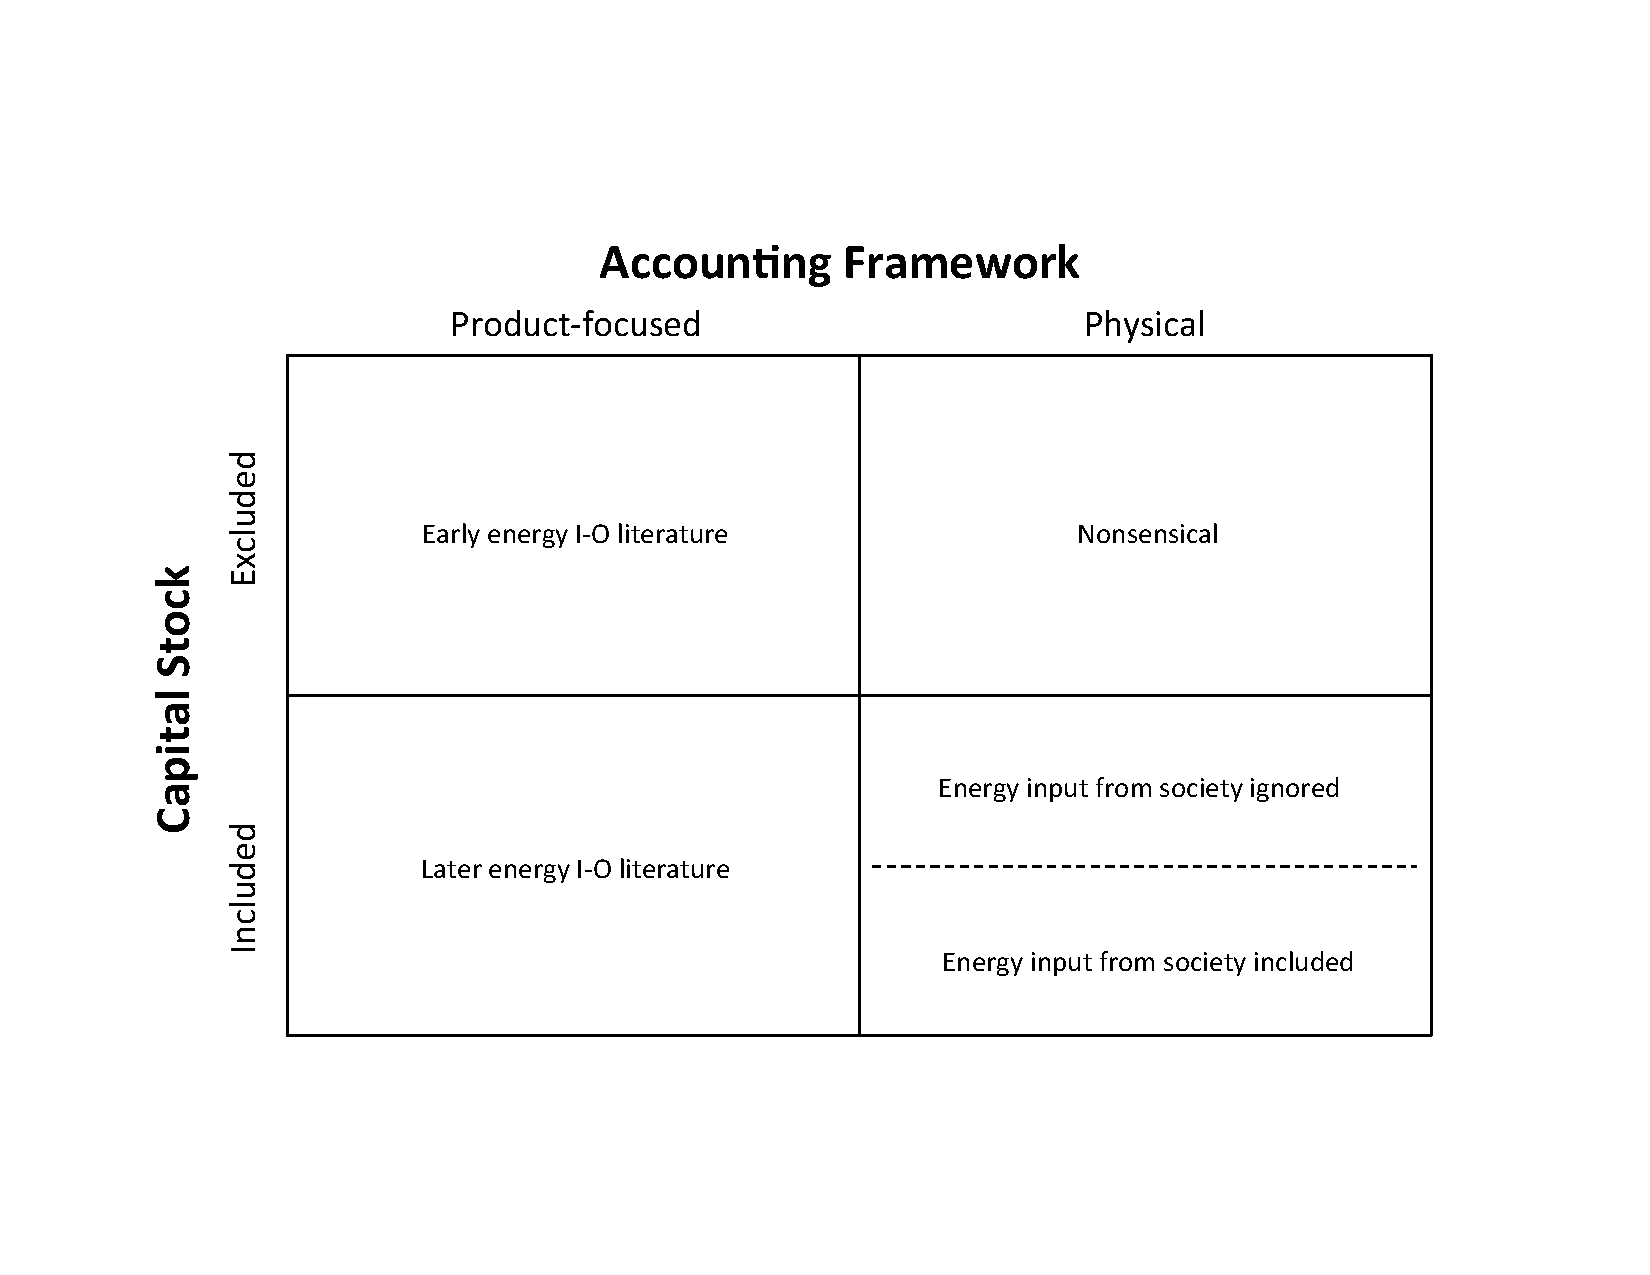
\includegraphics[width=0.8\linewidth]{Part_3/Chapter_Implications/Images/Grid.pdf}
\caption[Coordinates of analysis for implications for the I-O method]{Coordinates of analysis for implications for the EI-O method.}
\label{fig:coords_of_analysis}
\end{figure}


%+++++++++ I-O implications: product-based vs. physical ++++++++++
\subsection{Product-based vs.\ physical approaches}
\label{sec:prod_vs_physical}
%+++++++++

The distinction between product-focused and physical
accounting frameworks is located in the columns
of Figure~\ref{fig:coords_of_analysis}.
A \emph{physical accounting} framework strictly follows materials 
through the economy. 
Embodied energy is allocated to the material stock or material flow
in which it resides---wherever it goes, so goes the embodied energy. 
When the material is scrapped, so is its embodied energy.
For example, energy embodied within wastes ($\vec{B}_{waste}$) 
is not assigned to economic products. 
Rather, the energy embodied in wastes flows out of sectors 
into the biosphere \emph{with the waste material}.
In contrast, a \emph{product-focused accounting} framework assigns 
energy embodied in wastes to the products of the sector.
Both product-based and physical accounting frameworks
assign direct energy ($\dot{E}$) consumed by each sector
to the products of each sector.

Equation~\ref{eq:B_prod_physical_excluding_K} below
describes the outflow of embodied energy from sector $j$, 
for a physical accounting system 
that neglects both capital stock accumulation
and capital inflow (upper-right quadrant of
Figure~\ref{fig:coords_of_analysis}).\footnote{Equation~\ref{eq:B_prod_physical_excluding_K} 
	is used for illustrative purposes only. 
	A physical accounting framework would necessarily 
	include both flows and stocks of capital.
	Thus, the upper-right quadrant of Figure~\ref{fig:coords_of_analysis}
	(physical accounting framework that neglects capital)
	is labeled as nonsensical.}

\begin{equation} \label{eq:B_prod_physical_excluding_K}
	\dot{B}_{j}^{'}
	= \sum\limits_{i=1}^{n} \dot{B}_{ij}^{'} 
	- \dot{B}_{waste,j}
	+ \dot{Q}_{j0}
\end{equation}

\noindent{}Terms written with a ``prime''
(e.g.~$\dot{B}_{j}^{'}$) indicate definitions and terms that 
exclude input capital flows~($\dot{K}$) and capital stock~($K$).
The term~$\dot{B}_{waste,j}$ represents the energy embodied 
within wasted resource~($\dot{R}_{j0}$) 
and short-lived~($\dot{S}_{j0}$) material flows.
The $\dot{B}_{waste,j}$ term is subtracted, because waste material flows \emph{out of}
the sector. 
In a physical accounting framework, the energy embodied 
in waste flows ($\dot{B}_{waste,j}$)
is not assigned to the product~($\dot{B}_{j}^{'}$).

In contrast, Equation~\ref{eq:B_prod_product_excluding_K} describes the outflow 
of embodied energy from sector~$j$,
exclusive of capital stock,
for a product-focused accounting framework 
(upper left quadrant of Figure~\ref{fig:coords_of_analysis}).

\begin{equation} \label{eq:B_prod_product_excluding_K}
	\dot{B}_{j}^{'}
	= \sum\limits_{i=1}^{n} \dot{B}_{ij}^{'} 
	+ \dot{Q}_{j0}
\end{equation}

\noindent{}Notice that Equation~\ref{eq:B_prod_product_excluding_K} 
does not subtract the energy embodied in waste resource and short-lived material
flows ($\dot{B}_{waste,j}$) on the right side of the equation, 
because product-focused accounting systems assign energy embodied in wastes
to products.


%+++++++++ I-O implications: Capital stock ++++++++++
\subsection{Capital flows and stock}
\label{sec:capital_stock}
%+++++++++

The rows of Figure~\ref{fig:coords_of_analysis}
represent the role of capital flows and stock in an accounting framework.
The BEA Industry Accounts 
include capital flows in the ``make''
tables for each industry~\cite[Table~1]{Streitwieser:2011aa}, 
but capital inflows are accounted separately 
from intermediate uses as 
``Private fixed invest­ment''~\cite[Table~2]{Streitwieser:2011aa}.
During the earliest years of the EI-O method 
(prior to the mid-1970s) 
both capital inflows to economic sectors 
and stocks of capital were ignored.
In essence, the state of the art was located in the upper-left quadrant
of Figure~\ref{fig:coords_of_analysis}.
In time, Kirkpatrick~\cite{Kirkpatrick:1974te}, 
Bullard and Herendeen~\cite{Bullard-III:1975aa},
and Casler~\cite{Casler:1983uy} attempted to 
include inflows of capital in a product-focused
accounting framework, thereby moving the state of the art 
to the lower-left quadrant of Figure~\ref{fig:coords_of_analysis}.

We agree with this move, because of the many ways in which
capital stock is important for economies.
We can use the work of Eugene Odum~\cite{Odum1969}
to explain the importance of capital stock
within ecosystems,
and we have Herman Daly to thank
for making the connection between
ecosystems and economies.\cite{Daly1995}

In 1969, Odum outlined a number of 
defining characteristics of both \emph{developmental}
(growing) and \emph{mature} (stable) ecosystems in terms of key
properties of the system.\cite{Odum1969}
Ecosystems cannot
grow indefinitely in their (photosynthetic)~production rate~($P$)
due to the necessity of increasing maintenance
demands as the stock of biomass~($B$) increases.
Eventually, all production is used in this manner
and growth ceases 
$\left(\frac{\mathrm{d}}{\mathrm{d}t}(P) = 0\right)$.

In the early stages of ecosystem development,
the energy production rate 
per unit of biomass stock~$\left( \frac{P}{B} \right)$
is high.
As the ecosystem approaches maturity,
this ratio decreases.
Put another way,
the biomass stock (maintained) per unit of energy produced
$\left( \mathrm{the \; inverse \; ratio, \;} \frac{B}{P} \right)$
starts low and asymptotically increases to a maximum
when growth (in both $P$ and $B$) has ceased. 
The value of $\frac{B}{P}$ at the asymptote may be high or low\footnote{The
	value of $\frac{B}{P}$ at maturity (and the time taken to reach it)
	``may vary not only with different climatic 
	and physiographic situations but also with
	different ecosystem attributes in the same physical 
	environment.''~\cite[p.263]{Odum1969}}
and may therefore be considered a measure of 
the ``efficiency'' to which the ecosystem applies
energy production toward
the goal of maintaining biomass stock.
 
Turning back to economies,
Daly has, in our view,
correctly applied this concept to societal patterns
of economic consumption.\cite{Daly1995}
Our framework analogously suggests that
as capital stock~($\vec{B}_{K}$) increases,
an increasing flow of energy supply~($\vec{E}_{0}$)
will be needed to maintain that stock.\footnote{Today's economies 
	(and economic models and economic assumptions) are still focused
	on the objective of growth.
	If energy supply rates ($\vec{E}_{0}$) are constrained,
	these dynamics provide a possible reason for the difficulty
	of maintaining high levels of economic growth
	in mature economies.
	Eventually,
	we must learn to maximize the $\frac{B}{P}$
	ratios of our economies 
	$\left(\frac{\vec{B}_{K}}{\vec{E}_{0}}\right)$.}
Thus, it is important to account for capital stock in 
a material, energy, and value accounting framework.

To see the effect of the move from the upper-left to the lower-left
quadrant of Figure~\ref{fig:coords_of_analysis}, 
it is important to understand clearly both the assumptions and data that were used.
Energy analysts in the mid-1970s were utilizing the BEA
I-O tables,
which include capital flows on the output, but do not include capital flows on the input. 
Thus, this early literature implicitly assumes that 

\begin{equation} \label{eq:a_prime_lit}
	a_{ij}^{'} 
	\equiv \frac{\dot{X}_{\dot{R}_{ij}} + \dot{X}_{\dot{S}_{ij}}}
				{\dot{X}_{\dot{R}_{j}} + \dot{X}_{\dot{S}_{j}} + \dot{X}_{\dot{K}_{j}}}
	= \frac{\dot{X}_{ij}^{'}}{\dot{X}_{j}}.
\end{equation}

\noindent{}Comparison between Equations~\ref{eq:aij_def_expanded}
and~\ref{eq:a_prime_lit}
highlights the fact that the early literature neglects flows of capital stock
($\dot{X}_{\dot{K}_{ij}}$) on the input.
Thus, the Input-Output matrix in the early EI-O literature
($\vec{A^{'}}$) is

\begin{equation} \label{eq:A_matrix_def_literature}
	\vec{A}^{'} 
	=
	\begin{bmatrix}
		a_{22}^{'} & a_{23}^{'}	\\[4pt]   % [4pt] gives a little extra vertical space.
		a_{32}^{'} & a_{33}^{'}	
	\end{bmatrix}.
\end{equation}

% \noindent{}Furthermore, the early literature implicitly defines 
% energy intensity as
% 
% \begin{equation}
% 	\varepsilon_{j}^{'} 
% 	= \frac{\dot{T}_{j}^{'}}{\dot{X}_{j}^{'}},
% \end{equation}
% 
% \noindent{}with
% 
% \begin{equation}
% 	\dot{T}_{j}^{'} \equiv \dot{T}_{\dot{R}_{j}} + \dot{T}_{\dot{S}_{j}}
% \end{equation}
% 
% \noindent{}and
% 
% \begin{equation}
% 	\dot{X}_{j}^{'} \equiv \dot{X}_{\dot{R}_{j}} + \dot{X}_{\dot{S}_{j}}.
% \end{equation}
% 
% \noindent{}The above equations implicitly ignore both value and energy embodied within
% flows of capital.
% \noindent{}In contrast, our framework (Equation~\ref{eq:X_hat_matrix_def})
% includes capital flows explicitly:
% 
% \begin{equation}
% 	\hat{\vec{X}} = \hat{\vec{X}}_{\dot{R}} + \hat{\vec{X}}_{\dot{S}} + \hat{\vec{X}}_{\dot{K}}.
% \end{equation}
% 
The implicit assumptions of the early energy I-O literature 
are consistent with the upper-left quadrant
of Figure~\ref{fig:coords_of_analysis}, 
and the energy intensity equation
found in most of the early literature is

\begin{equation} \label{eq:intensity_upper_left}
	\boldsymbol{\varepsilon}^{'}
	= {\left( \vec{I} - {\vec{A}^{'}}^{\mathrm{T}} \right)}^{-1}
		{\left( \hat{\vec{X}} \right)}^{-1}
		\vec{E}_{0}.
\end{equation}

Bullard and Herendeen~\cite{Bullard-III:1975aa}, 
following Kirkpatrick~\cite{Kirkpatrick:1974te},
added flows of capital as inputs 
to each sector~\cite[Figure~5]{Bullard-III:1975aa},
and, in so doing, changed Equation~\ref{eq:intensity_upper_left}
to Equation~\ref{eq:intensity_lower_left}:

\begin{equation} \label{eq:intensity_lower_left}
	\boldsymbol{\varepsilon}
	= {\left[ \vec{I} - 
			\left( {\vec{A}^{'}}^{\mathrm{T}} 
					+ \vec{A}_{\dot{K}}^{\mathrm{T}} \right) \right]}^{-1}
		{\left( \hat{\vec{X}} \right)}^{-1}	\vec{E}_{0}
\end{equation}

\noindent{}with

\begin{equation}
	\vec{A}_{\dot{K}}
	\equiv
	\begin{bmatrix}
		a_{\dot{K}_{22}}	& a_{\dot{K}_{23}} \\
		a_{\dot{K}_{32}}    & a_{\dot{K}_{33}} \\
	\end{bmatrix}
\end{equation}

\noindent{}and

\begin{equation}
	a_{\dot{K}_{ij}}
	\equiv
	\frac{\dot{X}_{\dot{K}_{ij}}}{\dot{X}_{j}}.
\end{equation}

Bullard and Herendeen
counted embodied energy 
from incoming capital stock in $\vec{A}_{\dot{K}}$ 
only if it was used
for replacement.\cite[p.~488]{Bullard-III:1975aa}
Consequently, they did not count incoming energy embodied 
in capital if the incoming capital was used 
to increase the stock of capital within a sector.
In fact, Bullard and Herendeen's
product-focused accounting framework
did not include an embodied energy stock 
for economic sectors~($\vec{B}$) at all.
They assumed that half of the incoming capital 
went toward replacement.
These early researchers moved from the upper-left quadrant
to the lower-left quadrant of Figure~\ref{fig:coords_of_analysis}.
And, Equation~\ref{eq:intensity_lower_left} represents 
a partial step toward developing 
a method for estimating energy intensity ($\boldsymbol{\varepsilon}$)
that fully accounts for capital stock.

As stated above, we agree with Kirkpatrick~\cite{Kirkpatrick:1974te}, 
Bullard and Herendeen~\cite{Bullard-III:1975aa},
and Casler~\cite{Casler:1983uy} that incoming capital
is important and should be included in an accounting framework
(i.e., we should be on the lower half of Figure~\ref{fig:coords_of_analysis}).
But, we recommend that inclusion of incoming capital should
be done within a \emph{physical} accounting framework, 
i.e.\ we should make a second move from the lower-left to the lower-right
quadrant of Figure~\ref{fig:coords_of_analysis}.
Specifically, incoming capital should be included 
not only on incoming material streams but also
as a stock that can accumulate within the economic sector itself.

Our recommendation is informed by the work of 
Odum~\cite{Odum1969} and Daly~\cite{Daly1995}
and is based on the belief that
accounting for stocks of capital is important for developing a coherent view
of the structure of an economy. 
Stocks of capital are essential to the production process:
without machines and factories, cars cannot be produced. 
And, in industrialized economies 
maintenance of captial stock becomes an important 
driver of demand.
Thus, the buildup of capital stock (and associated embodied energy) 
within economic sectors is an essential aspect of industrialization.
Carefully tracking (on a physical, as opposed to financial, basis) 
capital stock in each economic sector is essential 
for understanding the network effects of 
upstream energy demand as new industries and products arise 
(e.g., electric vehicles). 

In a physical accounting system that includes capital stock
(lower-right quadrant of Figure~\ref{fig:coords_of_analysis}), 
energy embodied within accumulated capital stock
is not assigned to products ($\vec{P}$); 
rather, accumulated embodied energy is assigned to a stock of embodied energy
for each sector ($\vec{B}_{K}$).
And, the stock of embodied energy ($\vec{B}_{K}$)
can depreciate.

A physical accounting framework that fully includes capital stock
(lower-right quadrant of Figure~\ref{fig:coords_of_analysis}) 
is described by Equation~\ref{eq:intensity_lower_right_no_society}. 

\begin{equation} \label{eq:intensity_lower_right_no_society}
	\boldsymbol{\varepsilon}
	= {\left( \vec{I} - {\vec{A}}^{\mathrm{T}} \right)}^{-1}
		{\left( \hat{\vec{X}}  \right)}^{-1}
		\left[ \vec{E}_{0}
			  - \frac{\mathrm{d}\vec{B}_{K}}{\mathrm{d}t}
			  - \vec{B}_{waste}
			  - \hat{\boldsymbol{\gamma}}_{B} \vec{B}_{K} \right].
\end{equation}

\noindent{}Differences between Equation~\ref{eq:intensity_lower_right_no_society}
and Equation~\ref{eq:intensity_lower_left} include:

\begin{itemize}
	\item{Equation~\ref{eq:intensity_lower_right_no_society} includes $\vec{A}$
	while Equation~\ref{eq:intensity_lower_left} splits $\vec{A}$ into
	$\vec{A}^{'}$ and $\vec{A}_{\dot{K}}$ (a difference in appearance only),}
	
	\item{Equation~\ref{eq:intensity_lower_right_no_society} subtracts
	accumulation $\left( \frac{\mathrm{d}\vec{B}_{K}}{\mathrm{d}t} \right)$
	of energy embodied in capital stock,
	because energy embodied in the stock of capital 
	for a sector ($B_{K_{j}}$)
	is assigned to products of the sector,}
	
	\item{Equation~\ref{eq:intensity_lower_right_no_society} subtracts
	waste ($\vec{B}_{waste}$),
	because energy embodied in waste products is not assigned to 
	products of the sector, and}

	\item{Equation~\ref{eq:intensity_lower_right_no_society} subtracts
	depreciation ($\hat{\boldsymbol{\gamma}}_{B} \vec{B}_{K}$)
	of energy embodied in capital stock,
	because energy embodied in depreciated capital ($\dot{B}_{\dot{K}_{j0}}$)
	is assigned to products of the sector.}
\end{itemize}

There are two topics related to Equation~\ref{eq:intensity_lower_right_no_society} 
that are worthy of consideration:
waste flows and an accounting equation for capital stock.


%--------- I-O implications: Capital stock: Waste ----------
\subsubsection{Waste flows}
\label{sec:waste_flows}
%---------

We are unaware of any estimates of the energy embodied in wasted
material in an economy ($\vec{B}_{waste}$).  
But, it may be possible to develop a metric for the resource material efficiency of an 
economic sector ($\eta_{\dot{R}}$),
i.e.\ the fraction of the material that actually makes it into the product, 
such that:

\begin{equation} \label{eq:manufacturing_effiency}
	\eta_{\dot{R}_{j}}
	\equiv \frac{\dot{P}_{j}}{\sum\limits_{i=1}^{n} \dot{R}_{ij}}.
\end{equation}

\noindent{}With the above definition, 
the scrap rate for resources could be expressed as
$(1~-~\eta_{\dot{R}}) \sum\limits_{i=1}^{n} \dot{R}_{ij}$.
Allwood et.\ al.~\cite[p. 193]{allwood2012sustainable} 
used a process-based approach to manufacturing efficiencies
for metals used in manufacturing. 
The data are summarized in Table~\ref{tab:scrap_rates}.

\begin{table}
\caption[Manufacturing efficiencies for selected goods]{Manufacturing efficiencies
($\eta_{\dot{R}}$, 
Equation~\ref{eq:manufacturing_effiency})
for selected manufactured goods.\cite{allwood2012sustainable}}
\begin{center}
\begin{tabular} {r @{\hspace{2em}} l}
	\toprule
	Product & $\eta_{\dot{R}}$ [\%] \\
	\midrule
	Steel I-beam             & 90 \\
	Car Door Panel           & 50 \\
	Aluminium Drink Can      & 50 \\
	Aircraft Wing Skin Panel & 10 \\
	\bottomrule
\end{tabular}
\end{center}
\label{tab:scrap_rates}
\end{table}

Furthermore, one could assume that the rate
of short-lived materials ($\dot{S}$) used by a sector could be given as a 
fraction of the resource ($\dot{R}$) use rate such that:

\begin{equation}
	\rho_{\dot{S}_{j}}
	\equiv \frac{\dot{S}_{j0}}{\sum\limits_{i=1}^{n} \dot{R}_{ij}}
	= \frac{\sum\limits_{i=1}^{n} \dot{S}_{ij}}{\sum\limits_{i=1}^{n} \dot{R}_{ij}}.
\end{equation}

With the above definitions, the waste resource rate from an economic sector
can be given as

\begin{equation}
	\dot{R}_{j0} + \dot{S}_{j0}
	= (1 - \eta_{\dot{R}_{j}} + \rho_{\dot{S}_{j}}) \sum\limits_{i=1}^{n} \dot{R}_{ij}.
\end{equation}

\noindent{}The embodied energy in the waste materials would need to be estimated
from the embodied energy of the incoming resource and short-lived material flows as

\begin{equation}
	\dot{B}_{waste,j}
	= \dot{B}_{\dot{R}_{j0}} + \dot{B}_{\dot{S}_{j0}}.
\end{equation}


%--------- I-O implications: Capital stock: capital accounting equation ----------
\subsubsection{Simplification via capital stock accounting equation}
\label{sec:capital_accounting}
%---------

A possible simplification to Equation~\ref{eq:intensity_lower_right_no_society}
can be obtained from a control volume around the stock of capital in sector $j$:

\begin{equation}
	\frac{\mathrm{d}B_{K_{j}}}{\mathrm{d}t}
	= \sum\limits_{i=1}^{n} \dot{B}_{\dot{K}_{ij}} 
	- \gamma_{B_{j}} B_{K_{j}}.
\end{equation}

We can express the incoming energy embodied in capital ($\sum_{i=1}^{n} \dot{B}_{\dot{K}_{ij}}$)
as a fraction ($\alpha_{B_{j}}$) of the capital stock ($B_{K_{j}}$) as

\begin{equation}
	\alpha_{B_{j}}
	\equiv 
	\frac{\sum\limits_{i=1}^{n} \dot{B}_{\dot{K}_{ij}}} {B_{K_{j}}}
\end{equation}

\noindent{}for $j \in [2,n]$.

\noindent{}Together with the Kronecker delta ($\delta_{ij}$), we can write

\begin{equation}
	\hat{\boldsymbol{\alpha}}_{B}
	\equiv
	\delta_{ij} \alpha_{B_{j}}
	=
	\begin{bmatrix}
		\alpha_{B_{2}}	& 0               \\
		0               & \alpha_{B_{3}}  \\
	\end{bmatrix}.
\end{equation}

\noindent{}Thus, the embodied energy accounting equation around
the stock of capital in the economy can be written in matrix form as

\begin{equation}
	\frac{\mathrm{d}\vec{B}_{K}}{\mathrm{d}t}
	= \hat{\boldsymbol{\alpha}}_{B} \vec{B}_{K}
	- \hat{\boldsymbol{\gamma}}_{B} \vec{B}_{K}.
\end{equation}

\noindent{}Rearranging slightly gives

\begin{equation} \label{eq:alpha_cap_stock}
	\hat{\boldsymbol{\alpha}}_{B} \vec{B}_{K}
	= \frac{\mathrm{d}\vec{B}_{K}}{\mathrm{d}t}
	+ \hat{\boldsymbol{\gamma}}_{B} \vec{B}_{K},
\end{equation}

\noindent{}which says that incoming capital ($\hat{\boldsymbol{\alpha}}_{B} \vec{B}_{K}$)
can be used to either
increase the stock of capital in the economy 
$\left( \frac{\mathrm{d}\vec{B}_{K}}{\mathrm{d}t} \right)$
or overcome depreciation ($\hat{\boldsymbol{\gamma}}_{B} \vec{B}_{K}$).
Substituting Equation~\ref{eq:alpha_cap_stock} into
Equation~\ref{eq:intensity_lower_right_no_society} gives

\begin{equation} \label{eq:epsilon_leontief_with_A_alpha}
	\boldsymbol{\varepsilon} 
	= {(\vec{I} - \vec{A}^{\mathrm{T}})}^{-1}\hat{\vec{X}}^{-1}
		\left[\vec{E}_{0} 
				- \hat{\boldsymbol{\alpha}}_{B} \vec{B}_{K}
				- \vec{B}_{waste}
		\right].
\end{equation}


%+++++++++ I-O implications: Energy input from society ++++++++++
\subsection{Energy input from society}
\label{sec:energy_from_society}
%+++++++++

In Sections~\ref{sec:prod_vs_physical}
and~\ref{sec:capital_stock} above,
we implicitly assumed that society 
(final consumption, Sector~1 in our example economies A--C) % chktex 8
contributes negligible energy to the economy.
Thus, all vectors and matrices in Equation~\ref{eq:intensity_lower_right_no_society}
involve Sectors~2--$n$, but not Sector~1.

Energy input from society to the economy ($\vec{T}_{1}$)
is ``muscle work'' supplied by working humans 
and draft animals.\cite{Ayres:2003ec,Ayres:2010ug,Warr:2012cg} 
This muscle work term ($\vec{T}_{1}$) should include
all upstream energy required to make the labor available.\footnote{At this point 
	in the development of our framework,
	we are assuming that Final Consumption (Sector 1) is exogenous to the economy 
	(Sectors 2\ldots{}$n$), 
	and upstream energy consumption needs to be included manually.
	However, in Section~\ref{sec:what_is_endogenous}, we show that Final Consumption
	can be endogenized.
	Once endogenized, the energy intensity of Final Consumption ($\varepsilon_{1}$) 
	will automatically include the upstream energy required to make labor available.
	(See Appendix~\ref{chap:infinite_series}.)

	It is important to note, too, that labor can have very high energy intensity, 
	because $\varepsilon_{1}$ includes the energy required to supply food 
	for and transport to workers.} 
Equation~\ref{eq:epsilon_leontief_with_A} 
adds the effect of energy input from society to the economy,
effectively moving from the top half to the lower half of the lower-right quadrant
in Figure~\ref{fig:coords_of_analysis}.

\begin{equation}
	\boldsymbol{\varepsilon} 
	= {(\vec{I} - \vec{A}^{\mathrm{T}})}^{-1}\hat{\vec{X}}^{-1}
		\left[\vec{E}_{0} 
				+ \vec{T}_{1} 
				- \frac{\mathrm{d}\vec{B}_{K}}{\mathrm{d}t} 
				- \vec{B}_{waste}
				- \hat{\boldsymbol{\gamma}}_{B}\vec{B}_{K}
		\right].\tag{\ref{eq:epsilon_leontief_with_A}}
\end{equation}

For industrialized economies, the direct energy component ($\vec{E}_{1}$) 
of muscle work ($\vec{T}_{1}$)
is likely to provide only a small fraction
of the energy input from fossil fuels ($\vec{E}_{0}$).
But, the embodied energy of the muscle work ($\vec{B}_{1}$) is likely to be large.
For agrarian
and developing economies, 
$\vec{T}_{1}$ and $\vec{E}_{0}$ 
could be on the same order of magnitude.
For both industrial and agrarian economies,
neglecting $\vec{T}_{1}$ could cause errors
in estimates of $\boldsymbol{\varepsilon}$.
To the extent that $\vec{T}_{1}$ 
is significant relative to $\vec{E}_{0}$,
neglecting $\vec{T}_{1}$
will underpredict the energy intensity of economic output.
Energy input from society is discussed further 
in Section~\ref{sec:what_is_endogenous}.


%+++++++++ I-O implications: Recommendation ++++++++++
\subsection{Recommendation}
\label{sec:I-O_recommendation}
%+++++++++

Sections~\ref{sec:prod_vs_physical}--\ref{sec:energy_from_society} 
discussed three factors that affect the form of the
energy intensity equation: 
product-focused vs.\ physical accounting frameworks,
whether capital stock is included, and
whether energy input from society is included.
The three factors are summarized in Figure~\ref{fig:coords_of_analysis}.

At this point, it is instructive to look back at the 
product-focused vs.\ physical discussion in Section~\ref{sec:prod_vs_physical}.
We understand the argument for including capital stock in a product-focused
accounting framework (lower-left quadrant of Figure~\ref{fig:coords_of_analysis}):
capital stock and waste exist 
solely due to product demand, 
therefore energy embodied in capital and waste should be assigned to products. 
However, a product-focused framework that includes capital stock (lower-left quadrant of
Figure~\ref{fig:coords_of_analysis})
masks structural aspects of economies
that we believe are essential to fully understanding how and why energy flows 
through economies, namely the accumulation of capital
and associated energy embodied within sectors.

The metabolic metaphor provides guidance here. 
If we were to create a model of an organism that neglects 
tissues that accumulate embodied energy,
the organism (in the model) has nothing with which to 
absorb, process, waste, or otherwise exchange
material with the biosphere.
The organism doesn't physically exist (in the model)!
Neglecting to account for the stock of capital (and its embodied energy) 
is tantamount to assuming that economic production occurs out of nothing!
Accounting for capital stock is essential.

For our framework, we chose a physical accounting approach
(which puts us in the right column of Figure~\ref{fig:coords_of_analysis}).
We chose the physical approach primarily because of our belief that 
capital is an important aspect of economies,
and the physical accounting framework
properly includes a stock of capital for each sector of the economy.
Product-based accounting frameworks mask crucial aspects 
of why and how energy flows through economies.
We acknowledge that the choice of a physical accounting framework necessitates
careful tracking of capital flows (and associated embodied energy)
through the economy. 
For more on data needs, see Section~\ref{sec:Data}.

Finally, we suggest that accounting for energy input from society
to the economy is important, 
and we need to be in the lower half of the bottom-right quadrant
of Figure~\ref{fig:coords_of_analysis}.
So, the state of the art has moved from the nascent energy I-O literature
located in the upper-left quadrant of Figure~\ref{fig:coords_of_analysis}
as represented by Equation~\ref{eq:intensity_upper_left}
through the lower-left quadrant of Figure~\ref{fig:coords_of_analysis}
as represented by Equation~\ref{eq:intensity_lower_left}
to the lower half of the bottom-right quadrant 
of Figure~\ref{fig:coords_of_analysis}
as represented by Equation~\ref{eq:epsilon_leontief_with_A}.

The implication of the detailed development of our framework
on the EI-O method is 
some suggested enhancements to the EI-O method, 
including

\begin{itemize}
	\item{conversion to a physical accounting framework such as the one we propose herein,}
	
	\item{physical (as opposed to financial) tracking 
	of accumulated capital stock within economic sectors,}
	
	\item{redefinition of $\vec{A}$ and $\boldsymbol{\varepsilon}$ to include
	embodied energy on inflows of material, and}
	
	\item{use of Equation~\ref{eq:epsilon_leontief_with_A} instead of
	Equations~\ref{eq:intensity_upper_left} or~\ref{eq:intensity_lower_left}
	for estimating energy intensity ($\boldsymbol{\varepsilon}$)
	of economic sectors within an economy.}
\end{itemize}
 

%%%%%%%%%% Implications %%%%%%%%%%
\section{Implications for economic growth}
\label{sec:implications_for_development}
%%%%%%%%%%

Across the world, economic health and well-being 
is measured almost exclusively 
by Gross Domestic Product (GDP). 
If GDP grows, the economy is said to be growing.\footnote{GDP 
	is not the only indicator of well-being available; 
	there are several other measures in use.
	The Human Development Index (HDI) is a globally accepted measure 
	that augments GDP with education and life expectancy.\cite{Malik:2013aa} 
	In the US, the state of Maryland has been tracking well-being 
	using the \emph{Genuine Progress Indicator} (MDGPI),
	which combines measures of economic transactions with 
	environmental and social costs.\cite{MDDNR:2013aa,Bagstad:2007aa} 
	The MDGPI is closely related to 
	Herman Daly's Index of Sustainable Economic Welfare (ISEW)
	which allows policy-makers to account for contributions of and impacts on 
	the natural environment.\cite{Daly:1994aa,MDDNR:2014ab}
	Another example is the Nation of Bhutan's \emph{Gross National Happiness} (GNH),
	a systematic, annual compliation 
		of survey and other data related to nine factors: 
		ecological diversity and resilience,
		psychological well-being,
		health,
		education, 
		culture, 
		time use, 
		good governance, 
		community vitality, and 
		living standards.\cite{Ura:2012aa,GNH:2014aa}
	These alternatives to GDP are slowly gaining acceptance, particularly
	as their valuation methods are strengthened.\cite{Lawn:2003aa}}
Our framework affords the opportunity to assess economic growth 
in several dimensions.
Viewing these dimensions through the lens of our framework 
illustrates some important points about measures 
of economic growth and well-being.

% We're not using this footnote, because we have moved 
% toward talking about ``growth'' and away from talking about ``development.''
% Economic ``development''\footnote{We choose 
% 	to use the word ``development'' to
% 	describe expanding economies, despite significant misgivings about the term. 
% 	The unambiguously positive connotations of the words ``development'' and ``developed''
% 	fail to capture the nuances of travel along economic development paths:
% 	there are so many ways in which life experience in ``developed'' countries 
% 	is both better and worse than life in ``developing'' countries.
% 	We hope to convey our misgivings by surrounding these words with quotation marks in this text.}
% 
With reference to Figure~\ref{fig:C_value}, GDP is calculated by

\begin{equation} \label{eq:GDP_def}
	GDP
	= \sum\limits_{j=2}^{n} \dot{X}_{j}
\end{equation}

\noindent{}where $n$ is the number of sectors in the economy.
Equation~\ref{eq:GDP_def} clearly shows that 
$GDP$ is a \emph{flow} of value in units of \$/year.

A second possible measure of economic well-being is a \emph{stock}, 
wealth:

\begin{equation} \label{eq:Dev_Integral_Wealth}
	X_{j}(t) 
	= X_{j}(0) 
	+ \int_{t=0}^{t=t} \frac{\mathrm{d}X_{j}}{\mathrm{d}t}\mathrm{d}t,
\end{equation}

\noindent{}where $j=1$ for societal wealth 
and $j \in [2,n]$ for corporate wealth, both measured in dollars.

As an economy grows,
sectors within the economy accumulate capital stock 
($K$, typically expressed in units of dollars)
and associated embodied energy 
($B_{K}$, expressed in units of joules).
If we turn this around, 
accumulation of embodied energy
in economic sectors and society 
could be considered a \emph{proxy} for growth.\footnote{Embodied energy 
	as a proxy for economic growth may be overly focused on capital stock, 
	therefore one-dimensional, and reductive, 
	but GDP and other measures are open to similar criticism.}
Equation~\ref{eq:Dev_Integral_Economy} indicates how accumulated
embodied energy in the capital stock 
of an economy ($\vec{B}_{K}$) could be calculated:

\begin{equation} \label{eq:Dev_Integral_Economy}
	\vec{B}_{K}(t) 
	= \vec{B}_{K}(0) 
	+ \int_{t=0}^{t=t} \frac{\mathrm{d}\vec{B}_{K}}{\mathrm{d}t}\mathrm{d}t,
\end{equation}

\noindent{}where $\vec{B}_{K}$ is given by Equation~\ref{eq:B_vec_def}.
Equation~\ref{eq:Dev_Integral_Economy} clearly shows
that energy embodied in capital ($\vec{B}_{K}$) 
is a \emph{stock} (in units of joules), not a flow.

The behavior of $\vec{B}_{K}$ 
with respect to
$\frac{\mathrm{d}\vec{B}_{K}}{\mathrm{d}t}$ 
is vitally important. 
As an economy transitions from agrarian to industrialized, 
its capital stock ($K$) and associated embodied energy ($B_{K}$)
grows ever larger. 
The outflow of depreciated capital stock and its associated embodied energy 
will occur at a faster rate, too.
As increasingly large amounts of energy are embodied 
in the capital stock of an economy ($B_{K}$), 
Equation~\ref{eq:matrix_leontief} shows that
increasingly large energy extraction rates ($\vec{E}_{0}$) 
are required to maintain capital stock 
in the sectors of the economy
to offset the effects of depreciation 
($\hat{\boldsymbol{\gamma}}_{B} \vec{B}_{K}$),
assuming that $\frac{\mathrm{d}\vec{B}_{K}}{\mathrm{d}t} \ge 0$ 
is desired. 

During a period of rapid industrialization and infrastructure build-out, 
we expect both GDP and energy embodied in the economy ($\vec{B}_{K}$)
to increase.
But, there is no guarantee that GDP and $\vec{B}_{K}$ move 
in the same direction at all times.
Industrialized economies may experience GDP growth while 
the stock of embodied energy in the economy ($\vec{B}_{K}$) remains nearly constant,
because the economy is running circles to overcome the effects of depreciation.

There can be a time lag between movements of GDP and $\vec{B}_{K}$, too.
At the beginning of an economic downturn (defined as prolonged GDP reduction),
capital stock and associated embodied energy ($\vec{B}_{K}$) will remain approximately constant:
GDP moves but $\vec{B}_{K}$ doesn't.
But as the GDP decline continues, 
maintenance flows for capital stock will be reduced.
If depreciation overtakes maintenance, $\vec{B}_{K}$ will decline. 

% This next paragraph is too speculative.
% We don't have evidence of this at this time.
% If economic decline is associated with significant external 
% infrastructure investment (such as occurred in post-colonial Africa),
% GDP may decrease 
% while the stock of energy embodied in the economy ($\vec{B}_{K}$) increases 
% due to foreign aid focused on infrastructure enhancement. 

``Extract and export'' economies may exhibit different dynamics.
GDP growth occurs as resources are extracted and sold, 
but $\vec{B}_{K}$ remains flat if that income is not 
invested back into the economy as capital. 
An example of this occured with rubber exports from the Amazon.
Per capita incomes increased by an order of magnitude 
from 1820 to 1900 during the rubber export boom. 
However, as Amazon rubber exports dropped in value
due to stiff competition from Asian rubber production, 
per capita incomes dropped precipitously back to original levels. 
Throughout this period, the capital stock, 
and presumably the stock of embodied energy ($\vec{B}_{K}$), 
remained nearly constant.\cite{bunker1984modes}

In fact, capital (represented by energy embodied in infrastructure, $\vec{B}_{K}$) and 
financial resources or wealth (represented by $X_{2 \ldots n}$) 
are complementary factors of production for economic processes. 
But, we can go further than linking physical capital with financial resources.
If capital~($\vec{B}_{K}$) is to be useful, we need financial resources
or currency~($\dot{X}$) to 
\begin{itemize}
	\item{purchase direct energy~($\dot{E}$) to power the capital,}
	
	\item{purchase resources~($\dot{R}$) to feed the capital, and}
	
	\item{pay workers~(represented 
	by societal energy input to the economy,~$\vec{T}_{1}$) 
	to operate the capital.}
\end{itemize}

Thus, economic growth could be considered a ``fully coupled'' problem:
understanding it requires breadth of knowledge and appreciation for 
interactions among many important factors.
Each factor discussed above 
($\dot{X}$, $X$, $\vec{B}_{K}$, $\dot{E}$, $\dot{R}$, and $\vec{T}_{1}$)
is necessary, but not sufficient, for economic growth.

Our framework serves to highlight several issues in economic growth. 
Should it be measured by a stock or a flow? 
Which measure is most appropriate? 
What roles do currency, capital stock, energy, resources, and labor
play in economic processes?
These are overlapping and complementary areas of inquiry, and
we encourage further research in all of these areas.


%%%%%%%%%% Implications %%%%%%%%%%
\section{Implications for recycling, reuse, and dematerialization}
\label{sec:recycling}
%%%%%%%%%%

Dematerialization is the idea that economic activity can be unlinked 
from material or energy demands.\cite{FischerKowalski:2011uo} 
One method for dematerializing an economy 
is reuse and recycling of materials from both
short-lived goods
$\left(\vec{B}_{waste}\right)$
and depreciated
capital stock~$\left(\hat{\boldsymbol{\gamma}}_{B}\vec{B}_{K}\right)$
that would otherwise have
been discarded to the biosphere.\footnote{The 
other prevailing theory in the economics literature, that
dematerialization will occur as the economy substitutes away from production of material goods 
toward information and services, has been strongly challenged 
by ecological economists.\cite{Bartelmus:2003vi,parrinello2004service}}

In Chapter~\ref{chap:intensity},
we defined the rate of accumulation 
of embodied energy within the economy
$\left(\frac{\mathrm{d}\vec{B}_{K}}{\mathrm{d}t}\right)$
by the following equation:

\begin{equation}
	\frac{\mathrm{d}\vec{B}_{K}}{\mathrm{d}t} 
	= \vec{E}_{0}
	+ \vec{T}_{1}
	+ \hat{\vec{X}} (\vec{A}^{\mathrm{T}} - \vec{I})\boldsymbol{\varepsilon} 
	- \vec{B}_{waste}
	- \hat{\boldsymbol{\gamma}}_{B}\vec{B}_{K}\tag{\ref{eq:matrix_leontief}}
\end{equation}

One effect of recycling is to reduce the magnitude 
of the waste 
$\left(\vec{B}_{waste}\right)$
and depreciation 
$\left(\hat{\boldsymbol{\gamma}}_{B}\right)$ terms.
As can be seen in Equation~\ref{eq:matrix_leontief},
reducing both $\vec{B}_{waste}$ 
and~$\hat{\boldsymbol{\gamma}}_{B}$, 
puts \emph{upward} pressure on the accumulation of 
energy embodied in capital stock
$\left(\frac{\mathrm{d}\vec{B}_{K}}{\mathrm{d}t}\right)$,
all other things being equal.

Recycling has a mixed effect on energy demand ($\vec{E}_{0}$). 
Because recycled materials can displace newly-produced material 
in the economy and society, 
recycling will tend to reduce energy demand ($\vec{E}_{0}$). 
However, recycling processes require energy to operate, 
thereby putting upward pressure on energy demand ($\vec{E}_{0}$). 
If the energetic cost of recycling is lower than 
the energetic cost of obtaining virgin materials, 
as is the case for many metals
(e.g.\ aluminum~\cite{Chapman1975}), 
the result is a net reduction of energy demand 
from the biosphere ($\vec{E}_{0}$). 
Berry and Fels found that recycling of the material in automobiles
would result in energy reduction of 12,640 kW-hr per vehicle.\cite[p.~15]{Berry:1973vo}
Therefore recycling will put \emph{downward} pressure on 
the growth of embodied energy in the economy
$\left(\frac{\mathrm{d}\vec{B}_{K}}{\mathrm{d}t}\right)$,
via reduced $\vec{E}_{0}$, all other things being equal. 

If recycling produces a net reduction in energy demand ($\vec{E}_{0}$), 
% i.e.\ if the effect of displaced production dominates over the effect 
% of energy consumed in recycling processes, 
the upward pressure on growth 
$\left(\frac{\mathrm{d}\vec{B}_{K}}{\mathrm{d}t}\right)$ 
from decrease in depreciation 
$\left(\hat{\boldsymbol{\gamma}}_{B}\right)$ 
and waste ($\vec{B}_{waste}$)
and the downward pressure on growth 
from net reduction in energy demand 
$\left(\vec{E}_{0}\right)$ 
can offset each other.
Under those conditions, 
the accumulation rate of energy embodied
in capital stock
$\left(\frac{\mathrm{d}\vec{B}_{K}}{\mathrm{d}t}\right)$ 
will remain near zero 
and total embodied energy 
$(\vec{B}_{K})$ will remain constant. 
In that scenario, 
dematerialization can occur: 
reduced material and energy input ($\vec{E}_{0}$) 
can be accompanied by 
no change in
the growth of the economy
$\left(\frac{\mathrm{d}\vec{B}_{K}}{\mathrm{d}t}\right)$.
However,
as will be discussed in Section~\ref{sec:material_quality},
recycled materials can never entirely replace
the need for virgin materials.


%%%%%%%%%% Implications %%%%%%%%%%
\section{Comparison to a steady-state economy}
\label{sec:SSE}
%%%%%%%%%%

\begin{quotation}
	Growth means larger jaws and a bigger digestive tract 
	for more rapidly converting more resources into more waste, 
	in the service of unexamined and frequently destructive 
	individual wants.
	Development means better digestion of a non-growing throughput, 
	and more worthy and satisfying goals to which our life energies 
	could be devoted.\cite{Daly:2012aa}
\end{quotation}

As discussed in Chapter~\ref{chap:intro},
the human economy is a subset of the biosphere, 
a finite, non-growing system.
Thus, the human economy cannot physically grow indefinitely.
The concept of a non-growing or ``steady-state'' economy
has existed for centuries.

There are a number of different
conditions that may characterize a system as steady-state.
In thermodynamics,
steady state is characterized by unchanging system properties ($p$),
such that $\left(\frac{\textrm{d}p}{\textrm{d}t}\right) = 0$.
In ecological economics, a steady-state
economy has been defined as a constant rate
of material throughput that maintains the stock
of ecological capital and provides a qualitatively well-lived life 
for the population.\cite[p.~32]{Daly1997}  
This definition is consistent
with zero rate of accumulation of stock. 
Ecological capital is not drawn down, 
nor is manufactured capital quantifiably increased. 
Increases in living standards result from economic ``development,'' 
in which qualitative 
improvement in life occurs through increases 
in ``efficiency, technology, and ethics.''~\cite[p.~167]{Daly1997} 

Two other conditions that might define a steady-state
economy are constant GDP or constant population.
Our framework, can address the first three steady-state conditions
(constant capital stock, constant throughput, and constant GDP).
The fourth condition (constant population) could be
accommodated with some adaptation of the 
framework. 
The issue of human population as part of society's
capital stock is addressed in Section~\ref{sec:people_as_stock}.


%+++++++++++++++++++++++++++++++++++++++++++
%+++++++++ Constant capital stock ++++++++++
%+++++++++++++++++++++++++++++++++++++++++++
\subsection{Constant level of capital stock}

In Chapter~\ref{chap:materials}, 
we introduced Equation~\ref{eq:C_CV_all_b}:

\begin{align}\tag{\ref{eq:C_CV_all_b}}
	- \frac{\mathrm{d}R_{0}}{\mathrm{d}t}										&
	=\sum_{j}\frac{\mathrm{d}K_{j}}{\mathrm{d}t}
	+ \sum_{i,j}\dot{S}_{ij}
	+ \sum_{j}\gamma_{K_{j}}K_{j}.
\end{align}

\noindent{}which indicates that 
natural resources in the 
biosphere~$\left(- \frac{\mathrm{d}R_{0}}{\mathrm{d}t}\right)$
are depleted by the economy
for the purposes of:

\begin{itemize}
	\item{increasing man-made capital stocks
	within the economy~$\left(\frac{\mathrm{d}K_{j}}{\mathrm{d}t}\right)$,}
	\item{providing short-lived goods exchanged within the
	economy~$\left(\dot{S}_{ij}\right)$, and}
	\item{overcoming depreciation of man-made
	capital stocks~$\left(\gamma_{K_{j}}K_{j}\right)$.}
\end{itemize}

Assuming,
first,
that a steady-state economy exists when the level
of capital stock remains constant
$\left(\sum_{j}\frac{\mathrm{d}K_{j}}{\mathrm{d}t}=0\right)$,\footnote{Note
that the steady-state condition does not preclude expansion
of some sectors of the economy, provided that there is 
equal contraction elsewhere.}
we can see that Equation~\ref{eq:C_CV_all_b}
reduces to:

\begin{align}\label{eq:C_CV_all_c}
	- \frac{\mathrm{d}R_{0}}{\mathrm{d}t}										&
	= \sum_{i,j}\dot{S}_{ij}
	+ \sum_{j}\gamma_{K_{j}}K_{j}.
\end{align}

A number of interesting concepts may be understood via
Equation~\ref{eq:C_CV_all_c}. 
Firstly,
if our steady-state economy is to be supported
sustainably,
then withdrawal of natural resources from the biosphere
$\left(\frac{\mathrm{d}R_{0}}{\mathrm{d}t}\right)$
had better be at some rate lower than the biosphere
can replenish those stocks. 
In reality, 
$\frac{\mathrm{d}R_{0}}{\mathrm{d}t}$
is really the sum of many different resources
(flora and fauna, water) each of which will have
its own natural rate of regeneration.
As such, 
the sustainability criterion  is a vector of values,
one for each natural resource, 
all of which be met individually.

Secondly,
the steady state condition 
$\left(\sum_{j}\frac{\mathrm{d}K_{j}}{\mathrm{d}t}=0\right)$
says nothing about the transfer rates of short-lived goods 
within in the economy $\left(\sum_{i,j}\dot{S}_{ij}\right)$
or the depreciation of capital stock back to the biopshere
$\left(\sum_{j}\gamma_{K_{j}}K_{j}\right)$.
Equation~\ref{eq:C_CV_all_c} indicates that 
the higher the rates of these flows,
the greater the rate of depletion of
natural resources, and the more difficult it will be to
meet the sustainability condition 
(that the withdrawal rate of natural resources from the biosphere
is lower than the biosphere
replenishment rate).
Within industrial society,
the flow of short-lived goods 
(packaging,
paper products,
disposable tableware,
cutlery,
and napkins)
is large,
and, presumably, attaining a sustainable steady-state economy
will be difficult.
This definition of steady state 
$\left(\sum_{j}\frac{\mathrm{d}K_{j}}{\mathrm{d}t}=0\right)$
does not necessarily coincide with sustainability.

As discussed in Chapter~\ref{chap:materials},
the rate of depreciation ($\gamma_{K}$) is inversely
proportional to the average lifetime of capital stock---as
the average lifetime of capital stock decreases,
the rate of depreciation of capital stock increases which
increases the draw on natural resources (by Equation~\ref{eq:C_CV_all_c}).
It is likely that the average lifetime of capital stock has
decreased over the last century, 
due to a decrease in durability of capital stock
(the average table built today is not as durable as the average table
built in the early twentieth century)
and also due to increasing proportions of consumer electronics
with short lifetimes (cell phones, laptops, tablets).
Decreasing lifetime causes higher rates of flow for
replacement materials.
In the absence of extreme recycling of materials,
these large replacement flows place large demands on
natural resources.

Thirdly,
the maintenance flows necessary to overcome
depreciation
$\left(\sum_{j}\gamma_{K_{j}}K_{j}\right)$
are proportional to the magnitude of the capital
stock ($K_{j}$).
As such,
a larger stock of capital requires
greater draw on natural resources and is thus harder
to maintain within any sustainability constraint.
These points emphasize that constant capital stock
(or analogously constant population)
is not a sufficient condition for environmental sustainability.


%++++++++++++++++++++++++++++++++++++++++
%+++++++++ Constant throughput ++++++++++
%++++++++++++++++++++++++++++++++++++++++
\subsection{Constant material throughput}

Herman Daly has placed great emphasis on a steady-state
economy as having a constant rate of material throughput 
\cite{Daly1977, Daly1997}
which, as discussed above, should be below biophysical limits
if sustainability is to be achieved.
This is often referred to as the ``scale'' issue---how 
large is the (currently growing) human economy in relation
to the finite, non-growing biosphere of which it is a sub-system?
Growth of the human economy must either displace other natural
ecosystems (replacing old growth forest with cultivated crops)
or deplete natural capital stocks, be they 
renewable (fisheries) or 
non-renewable (fossil fuels).
As shown in Figure~\ref{fig:C_materials},
material throughput is composed of two distinct processes:
exchange of material \emph{from} the biosphere 
\emph{into} the economy (extraction)
and exchange of material \emph{from} the economy
\emph{into} biosphere (waste and depreciation).
We may characterize constant material throughput
as either constant rate of extraction, constant rate of
waste disposal, or both.
In the language of our framework, we could write:

\begin{align}\label{eq:const_throughput}
	\frac{\mathrm{d}}{\mathrm{d}t}\left(\dot{R}_{0}\right)		&
	= 0																							\\
	\frac{\mathrm{d}}{\mathrm{d}t}\left(\dot{S}_{0}\right)		&
	= 0																						\\
	\sum\limits_{i}
			\left[
				\frac{\mathrm{d}}{\mathrm{d}t}\left(\dot{R}_{i0}\right)
				+ \frac{\mathrm{d}}{\mathrm{d}t}\left(\dot{S}_{i0}\right)
				+ \frac{\mathrm{d}}{\mathrm{d}t}\left(\dot{K}_{i0}\right)
			\right]																			&
	= 0.
\end{align}

The above equations say nothing about the level 
of man-made capital stock ($K$)
or the flow rate of short-lived goods ($\dot{S}$).
Thus, within the constant throughput constraint,
increasingly effective use of materials could
theoretically allow increasing accumulation
of man-made capital~($K$) 
and increasing flow of short-lived goods ($\dot{S}_{ij}$)
as society learns to use resources better.
Eventually,
physical limits would entail that capital
stock could no longer be increased.
Presumably,
society would desire that the throughput of
materials would be within levels that could
be sustained by the biosphere,
both at the input side---natural 
resources extracted at rates lower
than natural regeneration rates---and 
at the output side---wastes emitted 
at rates below which
the biosphere can assimilate.


%++++++++++++++++++++++++++++++++++++++++
%+++++++++ Constant GDP ++++++++++
%++++++++++++++++++++++++++++++++++++++++
\subsection{Constant GDP}

Although one definition of a steady-state economy is
based upon constant levels of \emph{material} throughput,
it is possible to examine the implications of constraining the \emph{value} of 
GDP to be constant.\footnote{This is a theoretical exercise, 
	as Daly takes great pains to be clear that 
	the steady-state economy is materially-based. ``It is not
	to be thought of as `zero growth in GNP'.''~\cite[p. 32]{Daly1997}}
Within our framework,
a condition of constant GDP would be
characterized by the following equation:

\begin{equation}\label{eq:const_GDP}
	\frac{\mathrm{d}}{\mathrm{d}t}\left(GDP\right)
	=	\sum\limits_{j}\frac{\mathrm{d}}{\mathrm{d}t}\left(\dot{X}_{j}\right)
	= 0.
\end{equation}

Because,
under the subjective theory of value,
no value is attributed to the flow of materials
to or from the biosphere,
it is unclear what impact constant GDP would have
on capital stock ($K$)
or material throughput
(both extraction and waste disposal).
If we constrained $\dot{R}_{0}$ and
$\dot{S}_{0}$, 
it is likely that economic growth would 
decrease or even become zero or negative
$\left(\frac{\mathrm{d}}{\mathrm{d}t}\left(GDP\right) \leq 0\right)$.
It is conceivable that constraining
economic growth may act to constrain
material throughput,
though this is certainly not assured.

Although constraining GDP may not achieve the desired restraint on material throughput,
increasing GDP may not produce a desired increase 
in material well-being, either. 
This is particularly 
true for countries that have already achieved high levels of wealth.  
Many authors argue that increasing GDP
no longer guarantees increasing welfare~\cite{G-R1975a, Wackernagel1996,
Cobb1999, Daly2006, Costanza2014} 
for two main reasons:
\begin{itemize}
	\item firstly, that the costs of growth in GDP (e.g., externalities 
           and defensive expenditures) outweigh any benefit 
	that comes from increasing GDP;\@ and
	
	\item secondly, that increased GDP 
	increases relative income inequality,
	which decreases welfare for both rich and poor 
	alike.\cite{Daly2006}
\end{itemize}

Indeed, it may be the case that at the margin an increase 
in GDP produces more ``illth'' than ``wealth,'' 
resulting
in ``uneconomic'' growth.\cite[p. 42]{Daly2006} 
Uneconomic growth is much more likely 
to occur in a wealthy society than in a poor one, 
according to the law of diminishing returns.\footnote{Measuring
whether or not growth is ``economic'' cannot be done 
with traditional measures, such as GDP, since there is no
debit column in the ledger for GDP\@.
However, alternative metrics, such as ISEW or GPI, can perform such a function.}
Thus, a case could be made for constraining GDP growth in wealthy countries 
so that resources may be allocated to poorer countries
where growth in GDP is still likely to be ``economic.''~\cite{Daly2006}


%****** Mik: Finish this section. 
%In terms of what a SSE would look like in the I-O framework, 
%at first blush, I would think that dB/dt = 0 is one aspect.  
%Also, with no growth, inflow rates = depreciation rates.  
%The larger that B is for any society, the larger E must be (to overcome depreciation).  
%To minimize E, hyper-recycling is probably useful.  
%Those are at least a place to start. ******
%
%****** In our discussion, 
%we also addressed the attempts at SSE from point of view of society. 
%In order to achieve this goal \emph{without} recycling, 
%the goods and services sector should have to increase extraction to offset decreasing ore grade, 
%the energy sector should have to increase extraction of energy 
%to allow increasing extraction (unless efficiency could make up the gap: unlikely) 
%in which case the SSE would be violated from these two and from the POV of the earth.
%******


%%%%%%%%%% Implications Summary %%%%%%%%%%
\section{Summary}
\label{sec:summary_implications}
%%%%%%%%%%

In this chapter, we discussed several implications that arise from 
the detailed development of our dynamic framework for material,
energy, and value accounting.
The first implications are for the EI-O method itself. 
We recommend a physical accounting framework that fully
accounts for capital stock and energy input from society 
(normally assumed to not provide direct energy to the economy).
We then discussed implications for economic ``growth,''
namely that economic growth could be considered a ``fully coupled'' problem: 
understanding it requires breadth of knowledge 
and appreciation for interactions among many important factors,
including financial capital, physical capital and associated embodied energy,
direct energy, resources, and societal inputs.
Each, alone, is necessary, but not sufficient, for economic growth.
We discussed implications for recycling and reuse of materials
as well as the concept of dematerialziation.
Finally, we viewed the concept of a steady-state economy through
the lens of our framework.
We found that there are many potential definitions of a steady-state economy,
none of which are fully satisfying when compared against the ideal 
of sustainability.

In the next chapter, we point to some unfinished business.


\bibliographystyle{unsrt}
\bibliography{../../EROI_review_v3}


% Always give a unique label
% and use \ref{<label>} for cross-references
% and \cite{<label>} for bibliographic references
% use \sectionmark{}
% to alter or adjust the section heading in the running head
%% Instead of simply listing headings of different levels we recommend to let every heading be followed by at least a short passage of text. Furtheron please use the \LaTeX\ automatism for all your cross-references and citations.

%% Please note that the first line of text that follows a heading is not indented, whereas the first lines of all subsequent paragraphs are.

%% Use the standard \verb|equation| environment to typeset your equations, e.g.
%
%% \begin{equation}
%% a \times b = c\;,
%% \end{equation}
%
%% however, for multiline equations we recommend to use the \verb|eqnarray|
%% environment\footnote{In physics texts please activate the class option \texttt{vecphys} to depict your vectors in \textbf{\itshape boldface-italic} type - as is customary for a wide range of physical subjects.}.
%% \begin{eqnarray}
%% a \times b = c \nonumber\\
%% \vec{a} \cdot \vec{b}=\vec{c}
%% \label{eq:01}
%% \end{eqnarray}

%% \subsection{Subsection Heading}
%% \label{subsec:2}
%% Instead of simply listing headings of different levels we recommend to let every heading be followed by at least a short passage of text. Furtheron please use the \LaTeX\ automatism for all your cross-references\index{cross-references} and citations\index{citations} as has already been described in Sect.~\ref{sec:2}.

%% \begin{quotation}
%% Please do not use quotation marks when quoting texts! Simply use the \verb|quotation| environment -- it will automatically render Springer's preferred layout.
%% \end{quotation}


%% \subsubsection{Subsubsection Heading}
%% Instead of simply listing headings of different levels we recommend to let every heading be followed by at least a short passage of text. Furtheron please use the \LaTeX\ automatism for all your cross-references and citations as has already been described in Sect.~\ref{subsec:2}, see also Fig.~\ref{fig:1}\footnote{If you copy text passages, figures, or tables from other works, you must obtain \textit{permission} from the copyright holder (usually the original publisher). Please enclose the signed permission with the manucript. The sources\index{permission to print} must be acknowledged either in the captions, as footnotes or in a separate section of the book.}

%% Please note that the first line of text that follows a heading is not indented, whereas the first lines of all subsequent paragraphs are.

% For figures use
%
%% \begin{figure}[b]
%% \sidecaption
% Use the relevant command for your figure-insertion program
% to insert the figure file.
% For example, with the option graphics use
%% \includegraphics[scale=.65]{figure}
%
% If not, use
%\picplace{5cm}{2cm} % Give the correct figure height and width in cm
%
%% \caption{If the width of the figure is less than 7.8 cm use the \texttt{sidecapion} command to flush the caption on the left side of the page. If the figure is positioned at the top of the page, align the sidecaption with the top of the figure -- to achieve this you simply need to use the optional argument \texttt{[t]} with the \texttt{sidecaption} command}
%% \label{fig:1}       % Give a unique label
%% \end{figure}


%% \paragraph{Paragraph Heading} %
%% Instead of simply listing headings of different levels we recommend to let every heading be followed by at least a short passage of text. Furtheron please use the \LaTeX\ automatism for all your cross-references and citations as has already been described in Sect.~\ref{sec:2}.

%% Please note that the first line of text that follows a heading is not indented, whereas the first lines of all subsequent paragraphs are.

%% For typesetting numbered lists we recommend to use the \verb|enumerate| environment -- it will automatically render Springer's preferred layout.

%% \begin{enumerate}
%% \item{Livelihood and survival mobility are oftentimes coutcomes of uneven socioeconomic development.}
%% \begin{enumerate}
%% \item{Livelihood and survival mobility are oftentimes coutcomes of uneven socioeconomic development.}
%% \item{Livelihood and survival mobility are oftentimes coutcomes of uneven socioeconomic development.}
%% \end{enumerate}
%% \item{Livelihood and survival mobility are oftentimes coutcomes of uneven socioeconomic development.}
%% \end{enumerate}


%% \subparagraph{Subparagraph Heading} In order to avoid simply listing headings of different levels we recommend to let every heading be followed by at least a short passage of text. Use the \LaTeX\ automatism for all your cross-references and citations as has already been described in Sect.~\ref{sec:2}, see also Fig.~\ref{fig:2}.

%% Please note that the first line of text that follows a heading is not indented, whereas the first lines of all subsequent paragraphs are.

%% For unnumbered list we recommend to use the \verb|itemize| environment -- it will automatically render Springer's preferred layout.

%% \begin{itemize}
%% \item{Livelihood and survival mobility are oftentimes coutcomes of uneven socioeconomic development, cf. Table~\ref{tab:1}.}
%% \begin{itemize}
%% \item{Livelihood and survival mobility are oftentimes coutcomes of uneven socioeconomic development.}
%% \item{Livelihood and survival mobility are oftentimes coutcomes of uneven socioeconomic development.}
%% \end{itemize}
%% \item{Livelihood and survival mobility are oftentimes coutcomes of uneven socioeconomic development.}
%% \end{itemize}

%% \begin{figure}[t]
%% \sidecaption[t]
% Use the relevant command for your figure-insertion program
% to insert the figure file.
% For example, with the option graphics use
%% \includegraphics[scale=.65]{figure}
%
% If not, use
%\picplace{5cm}{2cm} % Give the correct figure height and width in cm
%
%% \caption{Please write your figure caption here}
%% \label{fig:2}       % Give a unique label
%% \end{figure}

%% \runinhead{Run-in Heading Boldface Version} Use the \LaTeX\ automatism for all your cross-references and citations as has already been described in Sect.~\ref{sec:2}.

%% \subruninhead{Run-in Heading Italic Version} Use the \LaTeX\ automatism for all your cross-refer\-ences and citations as has already been described in Sect.~\ref{sec:2}\index{paragraph}.
% Use the \index{} command to code your index words
%
% For tables use
%
%% \begin{table}
%% \caption{Please write your table caption here}
%% \label{tab:1}       % Give a unique label
%
% For LaTeX tables use
%
%% \begin{tabular}{p{2cm}p{2.4cm}p{2cm}p{4.9cm}}
%% \hline\noalign{\smallskip}
%% Classes & Subclass & Length & Action Mechanism  \\
%% \noalign{\smallskip}\svhline\noalign{\smallskip}
%% Translation & mRNA$^a$  & 22 (19--25) & Translation repression, mRNA cleavage\\
%% Translation & mRNA cleavage & 21 & mRNA cleavage\\
%% Translation & mRNA  & 21--22 & mRNA cleavage\\
%%Translation & mRNA  & 24--26 & Histone and DNA Modification\\
%%\noalign{\smallskip}\hline\noalign{\smallskip}
%%\end{tabular}
%%$^a$ Table foot note (with superscript)
%%\end{table}
%
%% \section{Section Heading}
%%\label{sec:3}
% Always give a unique label
% and use \ref{<label>} for cross-references
% and \cite{<label>} for bibliographic references
% use \sectionmark{}
% to alter or adjust the section heading in the running head
%% Instead of simply listing headings of different levels we recommend to let every heading be followed by at least a short passage of text. Furtheron please use the \LaTeX\ automatism for all your cross-references and citations as has already been described in Sect.~\ref{sec:2}.

%% Please note that the first line of text that follows a heading is not indented, whereas the first lines of all subsequent paragraphs are.

%%If you want to list definitions or the like we recommend to use the Springer-enhanced \verb|description| environment -- it will automatically render Springer's preferred layout.

%%\begin{description}[Type 1]
%%\item[Type 1]{That addresses central themes pertainng to migration, health, and disease. In Sect.~\ref{sec:1}, Wilson discusses the role of human migration in infectious disease distributions and patterns.}
%%\item[Type 2]{That addresses central themes pertainng to migration, health, and disease. In Sect.~\ref{subsec:2}, Wilson discusses the role of human migration in infectious disease distributions and patterns.}
%%\end{description}

%%\subsection{Subsection Heading} %
%% In order to avoid simply listing headings of different levels we recommend to let every heading be followed by at least a short passage of text. Use the \LaTeX\ automatism for all your cross-references and citations citations as has already been described in Sect.~\ref{sec:2}.

%% Please note that the first line of text that follows a heading is not indented, whereas the first lines of all subsequent paragraphs are.

%% \begin{svgraybox}
%% If you want to emphasize complete paragraphs of texts we recommend to use the newly defined Springer class option \verb|graybox| and the newly defined environment \verb|svgraybox|. This will produce a 15 percent screened box 'behind' your text.

%% If you want to emphasize complete paragraphs of texts we recommend to use the newly defined Springer class option and environment \verb|svgraybox|. This will produce a 15 percent screened box 'behind' your text.
%% \end{svgraybox}


%% \subsubsection{Subsubsection Heading}
%%Instead of simply listing headings of different levels we recommend to let every heading be followed by at least a short passage of text. Furtheron please use the \LaTeX\ automatism for all your cross-references and citations as has already been described in Sect.~\ref{sec:2}.

%% Please note that the first line of text that follows a heading is not indented, whereas the first lines of all subsequent paragraphs are.

%% \begin{theorem}
%% Theorem text goes here.
%% \end{theorem}
%
% or
%
%% \begin{definition}
%% Definition text goes here.
%% \end{definition}

%% \begin{proof}
%\smartqed
%% Proof text goes here.
%% \qed
%% \end{proof}

%%\paragraph{Paragraph Heading} %
%% Instead of simply listing headings of different levels we recommend to let every heading be followed by at least a short passage of text. Furtheron please use the \LaTeX\ automatism for all your cross-references and citations as has already been described in Sect.~\ref{sec:2}.

%% Note that the first line of text that follows a heading is not indented, whereas the first lines of all subsequent paragraphs are.
%
% For built-in environments use
%
%%\begin{theorem}
%%Theorem text goes here.
%%\end{theorem}
%
%%\begin{definition}
%%Definition text goes here.
%%\end{definition}
%
%%\begin{proof}
%%\smartqed
%% Proof text goes here.
%%\qed
%%\end{proof}
%
%% \begin{acknowledgement}
%% If you want to include acknowledgments of assistance and the like at the end of an individual chapter please use the \verb|acknowledgement| environment -- it will automatically render Springer's preferred layout.
%% \end{acknowledgement}
%
%% \section*{Appendix}
%% \addcontentsline{toc}{section}{Appendix}
%
%% When placed at the end of a chapter or contribution (as opposed to at the end of the book), the numbering of tables, figures, and equations in the appendix section continues on from that in the main text. Hence please \textit{do not} use the \verb|appendix| command when writing an appendix at the end of your chapter or contribution. If there is only one the appendix is designated ``Appendix'', or ``Appendix 1'', or ``Appendix 2'', etc. if there is more than one.

%% \begin{equation}
%% a \times b = c
%% \end{equation}
% Problems or Exercises should be sorted chapterwise
%% \section*{Problems}
%% \addcontentsline{toc}{section}{Problems}
%
% Use the following environment.
% Don't forget to label each problem;
% the label is needed for the solutions' environment
%% \begin{prob}
%% \label{prob1}
%% A given problem or Excercise is described here. The
%% problem is described here. The problem is described here.
%% \end{prob}

%% \begin{prob}
%% \label{prob2}
%% \textbf{Problem Heading}\\
%% (a) The first part of the problem is described here.\\
%% (b) The second part of the problem is described here.
%% \end{prob}




%!TEX root = ../../Heun_Dale_Haney_A_dynamic_approach_to_input_output_modeling.tex
%%%%%%%%%%%%%%%%%%%%% chapter.tex %%%%%%%%%%%%%%%%%%%%%%%%%%%%%%%%%
%
% sample chapter
%
% Use this file as a template for your own input.
%
%%%%%%%%%%%%%%%%%%%%%%%% Springer-Verlag %%%%%%%%%%%%%%%%%%%%%%%%%%
%\motto{Use the template \emph{chapter.tex} to style the various elements of your chapter content.}
\motto{In a complex and wealthy country like the United States, 
providing information on the structure of the economy and the environment 
is an essential function of government. 
It deserves more support.~\emph{\cite[p.~49]{Nordhaus:1999aa}}

\hfill---\emph{William D. Nordhaus}}

%%%%%%%%%%%%%%%%%%%%%%%%%%%%%%%%%%%%%%%%%%%%%%%%%%%%%%%
%%%%%%%%%% Conceptual and Theoretical Isseus %%%%%%%%%%
%%%%%%%%%%%%%%%%%%%%%%%%%%%%%%%%%%%%%%%%%%%%%%%%%%%%%%%
\chapter{Unfinished Business: Practical, Methodological, and Theoretical Issues}
% Always give a unique label
\label{chap:unfinished_business}
% use \chaptermark{} to alter or adjust the chapter heading in the running head
\chaptermark{Issues}
%%%%%%%%%%%%%%%%%%%%%%%%%%%%%%%%%%
%%%%%%%%%%%%%%%%%%%%%%%%%%%%%%%%%%
%%%%%%%%%%%%%%%%%%%%%%%%%%%%%%%%%%

%% \abstract{Each chapter should be preceded by an abstract (10--15 lines long) that summarizes the content. The abstract will appear \textit{online} at \url{www.SpringerLink.com} and be available with unrestricted access. This allows unregistered users to read the abstract as a teaser for the complete chapter. As a general rule the abstracts will not appear in the printed version of your book unless it is the style of your particular book or that of the series to which your book belongs.\newline\indent
%% Please use the 'starred' version of the new Springer \texttt{abstract} command for typesetting the text of the online abstracts (cf. source file of this chapter template \texttt{abstract}) and include them with the source files of your manuscript. Use the plain \texttt{abstract} command if the abstract is also to appear in the printed version of the book.}

%% Use the template \emph{chapter.tex} together with the Springer document class SVMono (monograph-type books) or SVMult (edited books) to style the various elements of your chapter content in the Springer layout.

\abstract*{This chapter reviews our list of unfinished business.
We begin by reviewing our call for better data collection and reporting
and expanding the discussion of metaphors and models. 
Thereafter, we call for new approaches
to ascribe value to material flows between the economy and the biosphere.
The remainder of this chapter discusses several questions
and methodological issues, including
hybridized EI-O and process methods,
resource quality, and co-products.
Then, several questions were posed:
are people capital stock?
what about the Sun? and
what is endogenous?
In all of the these areas, we called for additional 
inquiry and research 
into the questions raised by our framework.}

****

Suggest changing name of this chapter to ``Discussion.''

****

With any endeavor of this magnitude, 
namely development and presentation 
of a comprehensive framework for economies of the world,
unfinished business is inevitable. 
This chapter discusses several 
practical, methodological, and theoretical issues
that should be addressed in the future.
On a practical level, additional data are needed 
to fully utilize the framework developed herein.
In terms of methodological issues, the issue of co-products 
needs to be addressed.  
Finally, several theoretical issues, including
theories of value,
material and energy quality, 
boundaries, and 
the Sun
are addressed.
We begin with the issue of data.


%We begin with metaphors and models.


% %%%%%%%%%% Metaphors and models %%%%%%%%%%
% \section{Metaphors and models}
% \label{sec:metaphors_and_models}
% %%%%%%%%%%
% 
% This section circles back to the discussion that began the book and re-examines
% the importance of metaphor in light of the implications in the previous chapter.
% Historically, mainstream economists have used the \emph{machine} metaphor
% to describe economies. 
% In fact, much of mathematical economic modeling today 
% relies upon mechanistic conceptual foundations whose roots 
% are in Newtonian physics
% and The Enlightenment.\footnote{The subfield 
% 	of longwave economic growth modeling, as an example, 
% 	uses mechanistic language to describe their equations. 
% 	Jones~\cite[pp.~6 \&~18]{Jones:2001wn} 
% 	refers to the ordinary differential equations 
% 	that describe births, deaths, and the production of ideas
% 	as ``laws of motion.''}
% If your metaphor is a machine, it makes sense to analyze economies
% with equations that describe machines.
% In the mainstream, such equations usually, but not exclusively or restrictively,
% are developed assuming that the economic machine is a \emph{isolated} system.
% 
% In this book, we take the strong position that economies are
% better-represented as open, organic organisms with active metabolisms.
% Many ecological economists, 
% who are predisposed to view the economy as metabolic,
% reject the use of mechanistic equations 
% to describe the economy, in part because such equations often assume a 
% machine that operates independently from the biosphere.
% Other ecological economists dismiss mainstream economics 
% and its mechanistic models out of hand. 
% For example, S{\"o}llner pejoratively says 
% ``The prime example of physics envy and the desire 
% to emulate the natural sciences is, of course, 
% neoclassical economics which was explicitly and purposefully 
% copied from classical mechanics.''~\cite[p. 178]{Sollner:1997wx}
% 
% But, it doesn't have to be this way.
% We claim that it is not the use of equations 
% and mathematical models themselves that is the problem.
% Rather, it is the application of such equations 
% to an assumed isolated system
% that is is worthy of criticism.
% Thus, our approach herein includes rigorous application of the 
% admittedly mechanistic accounting equations 
% for materials, energy, embodied energy, and economic value
% \emph{under the assumption of} and \emph{including} 
% vigorous and necessary interactions between
% the economy and the biosphere.
% 
% It is our hope that this book allows
% 
% \begin{itemize}
% 	\item{mainstream economists to see that}
% 	\begin{itemize}
% 		\item{the metabolism metaphor is apt because 
% 		interaction between the economy and the biosphere is 
% 		what drives economic growth and}
% 		\item{rigorous mechanistic models can and should include 
% 		interactions between the biosphere and the economy; and} 
% 	\end{itemize}
% 	\item{ecological economists to see that rigorous mathematical modeling
% 	is an important tool for understanding interactions
% 	between the economy and the biosphere.}
% \end{itemize}
% 
% We encourage both mainstream and ecological economists
% to embrace mathematical modeling of 
% material, 
% energy, 
% embodied energy, 
% and economic value flows
% both within the economy and between the economy and the biosphere
% as a valid method of inquiry for modern economics.
% And, we encourage continual assessment of our models and metaphors.
% The stories we tell ourselves about our world have a significant 
% impact on how we perceive the world.
% We had better get those right.


%%%%%%%%%% Data %%%%%%%%%%
\section{Data}
\label{sec:Data}
%%%%%%%%%%

**** 

Matt: move this section to Next Steps chapter.

****

In Chapter~\ref{chap:intro}, 
we noted the importance of ``counting''
materials, energy, and value as each flows through economies.  
Unfortunately, unless data on these flows 
is collected and disseminated routinely, 
such counting is impossible.
At several points in this manuscript,
we have noted the very practical issue of the
need for additional data, information, and analysis.

In Section~\ref{sec:materials_auto},
our attempt to account the physical flows of 
materials through the US auto industry was
severely hampered by the lack of any data on
material flows.
Work to account such flows is starting to be
addressed at the level of economies,
particularly within Europe.\cite{EUROSTAT2011}
This work needs to continue, but
sub-economy, inter-industry material accounts need to be developed, too.
Chapter~\ref{chap:intensity} noted the need to collect
data on human and draft animal physical work input to 
sectors of economies, espeically for those economies where 
muscle work is on the same order of magnitude 
as fossil fuel energy input.

The need for rigorous and accurate data
is all the more pressing in light of the need 
to track physical capital in sectors,
as suggested in Chapter~\ref{chap:intensity}.
If this accounting relies on process-type
analysis,
then there is a critical need for systematic
collection and public dissemination of such data.
Some of these data are available only in proprietary format;
e.g., the latest version of the ecoinvent database (v3)
contains detailed analysis of over 10,000 
processes.\cite{EcoInvent2012}
This is a fantastic effort, but more needs to be
done to bring this crucial information into the public arena.

Environmental economic accounting in the US national accounts is currently non-existent. 
It was suspended by congress after the first
tables were published and has been on hold for twenty years. 
The BEA developed the
Integrated Environmental and Economic Satellite Accounts 
to complement the national accounts and track the 
``interactions of the economy and the environment.''~\cite[p.~33]{BEA1994a} 
In 1994, the BEA published the first phase of tables, for subsoil resources, 
along with detailed economic accounting 
and environmental valuation methodology behind the new data.\cite{BEA1994a, BEA1994b} 
The first set of tables valued the stock of
subsoil assets: oil, gas, coal, metals, 
and some major nonfuel minerals for the years 1947 to 1991. Each
year of data included values for \emph{Opening stock}, 
\emph{Additons}, \emph{Depletion}, \emph{Revaluation adjustment}, 
and \emph{Closing stock}. 
Several alternative valuation methods were used to provide a range of estimates.

Unfortunately, Congress ordered the BEA
to suspend all work
on environmental accounting, including development of
additional accounts for renewable and environmental resources.  
Congress asked for an independent panel of scientists to review the 
BEA's methodology.
In 1999, the review panel submitted its thorough evaluation as well as its strong
recommendation that the BEA
be funded to continue its work.\cite{Nordhaus1999a}
William Nordhaus,
chair of the panel, summarized the panel's recommendations 
in the lead quote for this chapter, 
``In a complex and wealthy country like the United States, 
providing information on the structure of the economy and the environment 
is an essential function of government. 
It deserves more support.''~\cite[p.~49]{Nordhaus:1999aa}
Fifteen years later, Congress has yet to act on this recommendation 
and lift the embargo on environmental accounting.

The business axiom ``you can't control what you don't measure''
seems appropriate here. 
As the world confronts significant challenges
of material and energy supplies in the coming years,
it will be impossible to make wise decisions about
which materials to use,
which energy sources to develop, and 
which products to incentivize.

The lede quote for Chapter~\ref{chap:value}
(``We try to measure what we value. 
We come to value what we measure.''~\cite[p.~2]{Meadows:1998aa})
points out that we are not presently valuing highly enough
the important flows that describe our metabolic economies.
We add our voices to those encouraging governments and 
institutions to collect high-quality data on material 
and energy flows.


%%%%%%%%%% Theories of value %%%%%%%%%%
\section{Theories of value}
\label{sec:theory_of_value}
%%%%%%%%%%

****

Mik: move to Value chapter.

****

As stated in Chapter~\ref{chap:value}, mainstream economics assumes a
\emph{subjective} theory of value, 
in which value is determined by the relative ability 
of products to satisfy the wants of buyers and sellers alike.
However, a person's wants are malleable and are, in turn, formed within a 
``constellation of shared goals to which a society aspires.''~\cite{Costanza:2004we}
Thoughout history, economists (particularly the classicals) 
and non-economists have searched for an invariant, objective, 
\emph{intrinsic} determinant of value.\footnote{Following the ecological economics literature, 
	we use the term intrinsic in the sense of ``objective.'' Costanza~\cite{Costanza:2004we} 
	notes that a better term would be objective in order to avoid moral overtones associated 
	with the term intrinsic.} 
Adam Smith, Karl Marx, David Ricardo, and neo-Ricardian Piero Sraffa all proposed 
alternative determinants of value.  
Their proposed objective theories of value were based 
on identifying the primary input into production,
such as \emph{labor} (Marx) or \emph{land} (Malthus), 
and using that input in the sense of a numeraire, 
a way to measure value across the entire spectrum 
of goods and services in commensurate units.

Costanza~\cite{Costanza:2004we} makes the case for energy 
as the only truly primary input into production 
and thus an, or rather \emph{the}, objective determinant of value. 
On a global scale, he notes, (solar) energy 
(including that which is stored in fossil fuels) is 
the only primary input into production:
everything else is an intermediate input. 
Thus, free energy input to production (accounting for all upstream energy)
could be the basis for an objective (intrinsic), 
energy theory of value.\footnote{This line 
	of inquiry has yielded some interesting analysis of the amount 
	of solar energy required to run the economy. 
	See Section~\ref{sec:emergy} for further discussion of the concept of \emph{emergy}.}
However, mainstream economics has rejected an energy theory of value, 
in favor of the subjective theory of value discussed in Section~\ref{sec:Value_Methodology}.
Because energy intensity ($\boldsymbol{\varepsilon}$) 
and the Energy Input-Output (EI-O) method 
were significant aspects of the 
proposal for an energy theory of value, 
many mainstream economists spurn 
analyses aimed at determining~$\boldsymbol{\varepsilon}$.

In contrast, we observe that energy intensity 
does not necessarily lead to an energy theory of value
and claim that energy intensity is inherently useful
as a metric describing the energy pathways traveled by economic products.
Energy intensity can provide important information for purchasing decisions
in increasingly interconnected economies.

In the development of our framework, we used the subjective theory of value 
(i.e., value based on market prices at the time of transaction) 
for pragmatic, rather than philosophical, reasons.
We believe that the information and signals provided by markets and prices 
are not sufficient to guide economies situated within a ``full'' earth.
And, national economic accounting limits its focus to measuring value-added, 
but ignores that to which value is being added,
thereby distorting economic value flows. 
As easily accessible forms of energy (e.g.,  oil extracted from the Texas panhandle) 
are used up and more difficult locations must be tapped (e.g., Alaskan north slope) 
the economy appears to grow.
The ``value-added'' by human and manufactured capital increases, 
as humans must do more work to extract domestic energy sources. 
However, what is actually happening is that the stock 
of natural resource is diminishing, 
and the drawdown of natural capital is mis-measured by GDP as income.\cite[pp.~66~and~75]{Daly1997}

Therefore, as ``that to which value is added'' diminishes, 
economic growth begins to reach binding constraints. 
Identifying the optimal economic 
scale---rate of materials put through the economy---that 
is viable for the biosphere to handle becomes an optimization problem. 
However, this is an optimization 
problem that the market is unable to solve on its own. 

Our framework provides a natural starting place for extending 
existing economic analysis methods to better
guide economies situated within a ``full'' earth. 
Instead of turning to an energy theory of value,
a system of envrionmental-economic accounting 
could be put in place to estimate the value 
of flows to and from the biosphere.\footnote{As of this printing, 
	the System of Environmental-Economic Accounting (SEEA)~\cite{UNSEEA:aa}
	is in its third revision 
	using a process of global consultation. 
	This system contains internationally agreed-upon standards for quantifying value flows 
	to and from the biosphere. 
	SEEA is a system analogous to the System of National Accounts (SNA), 
	a framework for measuring economic value creation consistently across nations.} 
Such a system could be included in our framework
to reconnect the economy to the biosphere, 
and flows that were conspicuously 
absent from Figure~\ref{fig:basic_value} will
be included, as shown in Figure~\ref{fig:basic_value_with_biosphere_flows}.

\begin{figure}[ht!]
\centering\
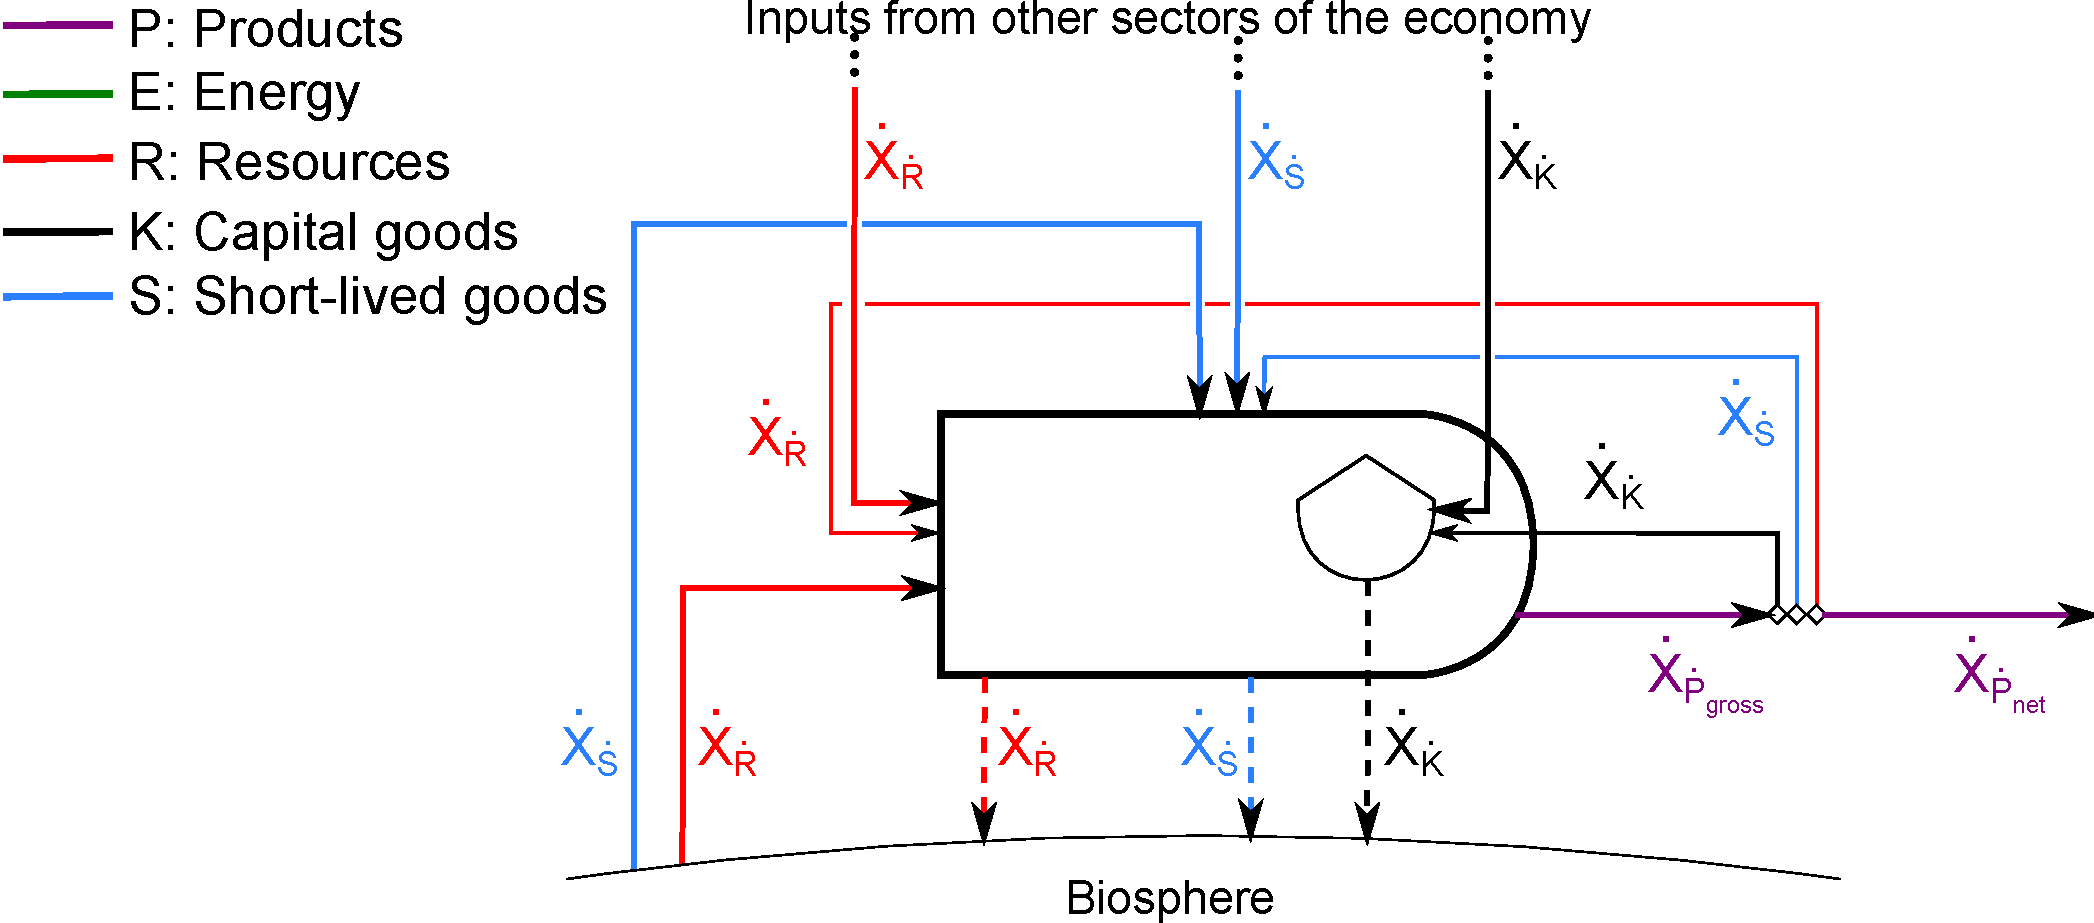
\includegraphics[width=0.8\linewidth]{Part_3/Chapter_Unfinished/images/PERKS_basic_unit_value_with_biosphere_flows.pdf}
\caption[Aggregated flows of value for a single sector including flows to and from the biosphere]{Aggregated flows of value for a single sector including flows to and from the biosphere.}
\label{fig:basic_value_with_biosphere_flows}
\end{figure}


%%%%%%%%%% Hybrid %%%%%%%%%%
\section{Hybrids of I-O and process-based methods}
\label{sec:hybrid}
%%%%%%%%%%

**** 

Matt: Move most of this section to the Background section
of the energy intensity chapter (Section~\ref{sec:IO_background}).
Frame it as ``there are two ways to obtain energy intensity,
bottom-up and top-down.
Each has advantages and disadvantages.
There are also hybrid methods.
We focus on top-down in this chapter for the following reasons.''

We could move the material about the hybrid method having some merit to the 
summary of the intensity chapter (Section~\ref{sec:intensity_summary}). 

****

In early chapters,
we made the distinction between
process-based (often called ``bottom-up'') 
and Input-Output (often called ``top-down'')
analyses.
The advantages and disadvantages of each type
of analysis are outlined in Figure~\ref{fig:IO_vs_process}.

Process analysis is based on detailed technological
or engineering models of specific economic processes.
Model specification and data collection is arduous,
time-consuming,
and costly.
The aim of process analysis is to calculate the
energetic and material flows associated with the process
under study by disaggregating the process into
several components or sub-processes.
In reality,
any economic process exists as part of a complex network of
interacting processes that encompass the entire economy.
Bullard et al.\ said 
``each step in a process analysis may be viewed as 
an expansion of the system boundary 
(around the item being analyzed) 
into the economic system.''~\cite[p.~281]{Bullard:1978vd}
Figure~\ref{fig:Hybrid_boundary} shows that 
every process calls on every other process within the economy,
even if only minutely and indirectly at many steps removed.
Obviously,
the time, 
effort,
and cost involved with trying to model and
measure all of the flows involved becomes daunting
for even low numbers of interacting processes.
The decision of where to draw the boundary of
a process analysis is known in the 
lifecycle assessment literature as the 
\emph{truncation problem}.\cite{Suh2004}
One method to extend the comprehensiveness of process
analyses is to use a hybrid method,
utilizing data from an EI-O analysis to supplement the
missing data from the truncation of the process analysis.
The financial cost of goods and services identified by
the process analysis are converted to energy
(or material) flows via the EI-O method.
The truncation error is replaced by a smaller aggregation
error due to limitations of the EI-O 
method.\cite{Bullard:1978vd}
A variety of other hybrid methods exist which also aim to
overcome the limitations of either process or I-O method 
individually.\cite{Bullard:1978vd, Suh2004, Suh2002, 
Crawford2008, Zhai2010}

\begin{figure}[p]
\centering\
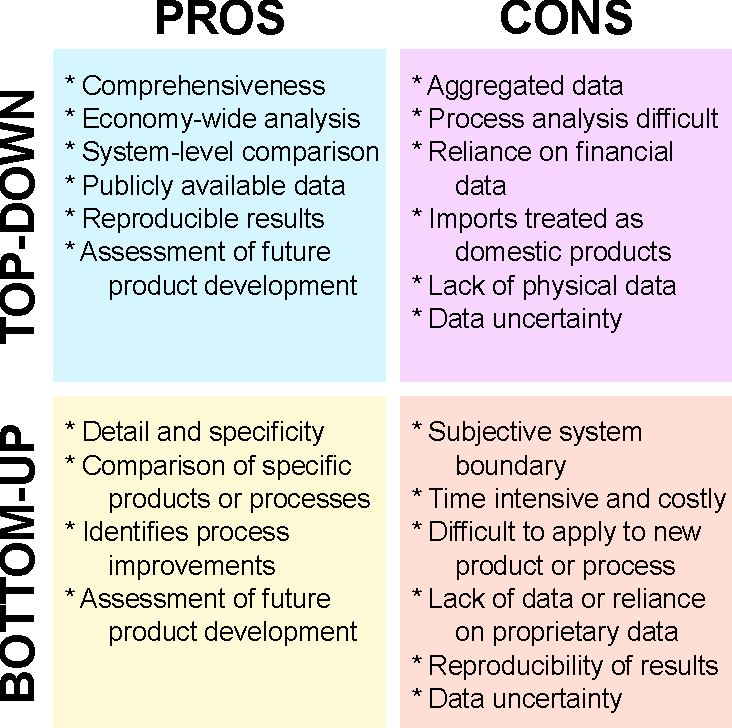
\includegraphics[width=0.8\linewidth]{Part_3/Chapter_Unfinished/images/Top_down_vs_bottom_up.pdf}
\caption[Top-down vs.\ bottom-up analyses]{Advantages (pros) and disadvantages (cons) of ``top-down,'' I-O and ``bottom-up,'' process-based analyses, adapted from~\cite{Hendrickson2006}.} % chktex 38
\label{fig:IO_vs_process}
\end{figure}

\begin{figure}[p]
\centering\
\includegraphics[width=\linewidth]{Part_3/Chapter_Unfinished/images/Hybrid_boundary.pdf}
\caption[System boundary for process and I-O analyses]{System boundary for process and I-O analyses, adapted from~\cite{Bullard:1978vd}.}
\label{fig:Hybrid_boundary}
\end{figure}

At several points in this book,
we noted the need to track accumulation of embodied
energy in sectors of the economy.
It may be that process-based methods are best for doing so.
However, we realize the limitations of process-based
methods (time, cost, etc.).
Perhaps hybrid methods can provide the necessary 
data without the high 
cost of a full process-based approach.


%%%%%%%%%% Second Law %%%%%%%%%%
\section{Resource quality and irreversibility}
\label{sec:resource_quality_and_irreversibility}
%%%%%%%%%%

%**** MCD - Talk about Red Queen here ****

The quality of both materials
and energy play a role in the 
efficiency with which economies 
convert material resources into products.

****

Matt: Move the following paragraph to the Introduction section
where EROI is discussed,
Section~\ref{sec:stall_non-renewable_stocks}.
Beware of duplication.
The introduction already discussed
the Best-First Principle, 
which this section was addressing 
without naming it.

****

Raw material and energy resources must first 
be extracted from the natural environment 
before they are utilized in the economy 
to provide goods and service to society. 
Despite increasing levels of technological efficiency, 
for example in consumer goods such as refrigerators and cars, 
evidence shows that 
the energy intensity of primary resource extraction, 
i.e.\ the energy required to extract raw materials 
from the environment, 
has been steadily increasing over 
the last fifty years.\cite{Hall1986, Mudd2010, Brandt2011} 
This increasing energy requirement for 
primary extraction means that 
less \textit{net energy} is available 
for downstream uses. 
%**** Mik---Add a discussion here that links 
%EROI (Chapter 3, Example B) with resource quality. ****
An important metric in this regard is
\emph{energy return on investment}~(EROI),
outlined in Section~\ref{sec:B_energy},
which measures the energy production
\emph{per unit} of energy investment by society.
As resource quality declines,
more energy is needed to extract resources,
EROI decreases,
and there is less net energy available to society.
If this decline in net energy availability 
outpaces technological advances in energy efficiency, 
there may be deleterious impacts on the 
economic output of the economy.
This need to increase productive capacity 
merely to maintain
the current level of production has been termed 
the ``Red Queen syndrome;''%
	\footnote{
	Of course,
	in any deck of cards there are two Red Queens.
	The other was described in Section~\ref{sec:capital_stock},
	regarding the increasing need to divert production
	to maintain capital stock.
	}
we must run faster and faster just to stay in place.\cite{Ross1988}



Within our framework, we do not account for either
the material or energetic quality of resources 
that pass through the economy nor the 
irreversibility of economic processes.
The following two subsections (\ref{sec:energy_quality}
and~\ref{sec:material_quality}) briefly discuss energy and material quality.
Thereafter, we raise the issue of thermodynamic irreversibility.



%+++++++++ Energy Quality ++++++++++
\subsection{Quality of energy}
\label{sec:energy_quality}
%+++++++++

****

Matt: move material from this section 
to the beginning of the Energy chapter~(Chapter~\ref{chap:direct_energy}).

****

The First Law of Thermodynamics
tells us that
the quantity of energy is conserved in every process.
The First Law
does not speak about the quality of energy---not
all forms of energy are equally \emph{useful}.
For instance,
a bath-full of water has as much thermal energy
as can be provided by a pint~(half liter) of
gasoline.\footnote{This assumes a 230 liter bath at
40$^\circ$ C,
i.e.\ 20$^\circ$ C above ambient.}
However, the gasoline is a much higher quality
store of energy than the water.
It is much more useful for performing tasks.

There are several ways to assess the quality of energy.
The Second Law of Thermodynamics provides, 
among other things,
a framework for discussing the \emph{quality} of energy.
Hammond and Winnett~\cite{Hammond:2009tu} reviewed
the influence of thermodynamics on ecological economics 
and noted the importance of the concept of \emph{exergy},
which combines the First
and Second
Laws of thermodynamics
to describe the maximum physical work 
which can be performed by an energy resource
in coming into equilibrium with its environment,
stating that exergy:

\begin{quote}
	represents the thermodynamic `quality' 
	of an energy carrier, 
	and that of the waste heat or energy lost in the reject stream. 
	Electricity, for instance, 
	may be regarded as an energy carrier having a high quality, 
	or exergy, because it can undertake work. 
	In contrast, low temperature hot water, 
	although also an energy [re]source, 
	can only be used for heating purposes. 
	This distinction between energy~(strictly enthalpy) 
	and exergy is very important 
	when considering a switch, for example, 
	from traditional internal combustion engines 
	to electric, hybrid, or fuel cell vehicles. 
	Thus, \ldots{} it is important to employ exergy analysis 
	alongside a traditional First Law energy analysis 
	in order to illuminate these issues.
\end{quote}

As such, exergy is a measure of how far a resource
is from thermodynamic equilibrium with its environment.
The further a resource is from equilibrium with the 
environment---the biosphere---the
higher the exergy and the higher the quality of the resource.

The quality of energy can be assessed in terms of economic value, too.
Some energy resources, such as liquid fuels, 
are more economically valuable than others,
i.e.\ within society, there is a preference for these resources,
such that, ``accounting for energy quality reveals a relatively strong relationship 
between energy use and economic output.''~\cite[p.~313]{Cleveland2000}
We see this preference played out on a daily basis
when coal is converted to electricity at 
an average efficiency of around one third.
Society is willing to pay a premium for electricity
over coal due to its vastly superior usefulness 
for a multitude of tasks.

%+++++++++ Material Quality ++++++++++
\subsection{Quality of materials}
\label{sec:material_quality}
%+++++++++

% **** Mik: Please review and add to this draft section. --Matt ****

%The concept of material quality has connections to our framework in two ways:
%\begin{enumerate}
%	\item 
%		first is Georgescu-Roegen's so-called 
%		``Fourth Law of Thermodynamics'';
%	\item		
%		second is (decline of) the quality of 
%		natural resources	within the biosphere.
%\end{enumerate}
%
%Georgescu-Roegen proposed a 
%Fourth Law of Thermodynamics
%\index{Fourth Law of Thermodynamics}
%which states that, ``In a closed system, 
%the material entropy must ultimately reach a maximum:'' 
%economic processes degrade material through wear and tear,
%just as energy.\cite{GeorgescuRoegen:1977tf}
%For example, consumption of coal to produce electricity
%results in CO$_2$ and ash that cannot
%be reprocessed into coal.
%Although mass (measured in kilograms) 
%is conserved through processes, 
%CO$_2$ and ash are significantly less useful than coal,
%and Georgescu-Roegen's ``Fourth Law'' 
%states that we need a way to account
%for the loss of material quality.
%
%The Fourth Law also states that,
%materials may never be recycled with 100\%
%efficiency, 
%hence to maintain a constant stock of material,
%some new resources must be imported into the system.
%In the case of the biosphere,
%materials are lost from the biosphere through
%the actions of tectonics and new materials are added
%via volcanic activity and erosion of rock by
%water, plants and animals.

****

Mik: move this subsection to the unlabeled beginning of the Materials chapter
(Chapter~\ref{chap:materials}) or to a new section (3.1.3) in the 
methodology section (Section~\ref{sec:Materials_Methodology}).

**** 



Similar to energy resources, 
non-energy resources 
have a range of quality, despite being conserved
in mass through every process.
An intact brick is of higher material quality---is of more use---than
after it has been ground to dust and scattered on the wind.
Society relies on material stocks or flows 
that have been concentrated by natural biophysical processes,
for example mineral seams or water courses. 
We do not mine desirable material from locations with
the average abundance of crustal materials.
As with energy,
we may measure the material quality of a resource
in reference to its environment,
in this case,
the average chemical composition of
its environment.
The more concentrated the resource,
the further it is from chemical equilibrium
with the environment and the higher the quality.
Again, exergy is a measure of this kind of quality.
The further a resource is from chemical equilibrium
with its environment,
the higher the exergetic content.

Additionally,
it takes more energy to process less concentrated resources
and more total material must flow through 
the process~(including overburden---the wasted portion that is extracted)
and the greater wear and tear on equipment.
This additional processing requirement entails that 
we will likely never mine average crustal abundance for needed
materials, or mine gold from seawater.
Furthermore,
it also entails that recycling---the act
of turning low quality materials into
high quality resources---requires energy
and degrades equipment.
The lower quality the waste,
the more energy and degradation occurs
such that
one hundred percent recycling of materials
is almost certainly practically (and possibly theoretically) 
impossible.
As such, 
we can deduce that the economy \emph{must always} be
a subsidiary of the biosphere, \emph{open} to
flows of materials both from (resources) and 
to (wastes) the biosphere.
This fact has direct implications for dematerialization
of our economies, 
which was discussed in reference
to our framework in Section~\ref{sec:recycling}.
There are fundamental limits to the amount
of material that must be directed to desired
end services.
For example, automobiles 
must have a minimum level of embodied materials.\footnote{Note
that this minimum is likely many times lower than the 
mass of current automobiles,
which are driven largely by preference.
The Rocky Mountain Institute has done some
work on the ultra-light, 
``hypercar'' concept.\cite{RMI1996}}
Despite the drive to dematerialization
and the apparent ``unhooking'' of the
material and energy intensity of GDP,
much of the dematerialization of ``developed'' 
nations has been by exporting manufacturing
to other countries.\cite{allwood2012sustainable}
The material footprint of OECD nations, 
when weighted by consumption, 
has increased significantly since 1990.\cite{Wiedmann2013}

%Furthermore, initial extraction of easy-to-reach ores 
%and fossil fuel resources (coal and oil)
%leads, over time, to a reduction in the quality 
%of material resources 
%(ore grades decrease over time).\cite{Mudd2010}
%As the quality of these resources degrades,
%greater amounts of energy must be expended
%(resulting in greater degradation of capital equipment)
%during their extraction.


%+++++++++ Irreversibility ++++++++++
% \subsection{Process irreversibility}
% \label{sec:irreversibility}
%+++++++++
%
% ****
%
% Suggest deleting this section.
%
% ****
%
%
% Our framework implicitly assumes,
% since we make no use of the Second Law,
% that all economic processes could be run in reverse;
% that products could be unmade into resources
% and that the energy and other short-lived material
% inputs would be spontaneously upgraded back into their
% original form.
% This of course is not true.
% Irreversibility is the concept that naturally-occurring processes
% are uni-directional in time.
% For example,
% bouncing a rubber ball heats it up;
% heating up a rubber ball does not cause it to
% spontaneously jump off the table.
% %the flow of electrical current through a resistor
% %generates heat;
% %however, pointing an operating hairdryer at an electrical resistor
% %does \emph{not} produce electricity.
%
% Considering the production of electricity from coal,
% we note that two important processes within a power plant are \emph{irreversible}:
%
% \begin{itemize}
% 	\item{the combustion process that converts coal to CO$_{2}$ and ash
% 	(with associated thermal energy release, $\dot{Q}$) and}
%
% 	\item{the heat transfer process wherein $\dot{Q}$ flows
% 	from high temperature to low temperature (with associated
% 	mechanical work production).\footnote{Note
% 		that the process of generating
% 		electricity via mechanical work is (at least in theory) a
% 		\emph{reversible} process.
% 		The generator could be run as a motor by electricity to produce
% 		mechanical work.
% 		In theory,
% 		electrical work and mechanical work are fully exchangeable;
% 		in reality, efficiency losses mean this is not quite the case.}}
% \end{itemize}
%
% \noindent{}Thermal energy does not spontaneously flow from low temperature to high temperature.
% Neither do ash and CO$_{2}$ spontaneously combine to form coal.
%
% The concepts of resource quality and irreversibility are inextricably linked.
% One statement of the Second Law
% indicates that heat flow is irreversible:
% it flows only from hot to cold.
% Because lower-temperature heat is less useful,
% we say that the thermal energy has
% degraded when it has been used~(comes
% into equilibrium with the environment).
% Again,
% exergy is a measure of irreversibility of processes.
% Exergy cannot be created, it can only be destroyed,
% hence a process is \emph{irreversible}
% if exergy is destroyed during the process.\footnote{The concept of
% irreversibility is often discussed in terms of \emph{entropy},
% which can only be created and cannot be destroyed.
% A process that generates entropy is said to be irreversible
% and all real processes generate entropy.}
%
% %The proposed Fourth Law is similar:
% %materials are degraded through their use.
% %Georgescu-Roegen's proposed Fourth Law establishes an analogy between
% %(a) the Second Law of Thermodynamics,
% %in which energy quality degrades with use and
% %(b) the Fourth Law of Thermodynamics,
% %in which material quality degrades with use.\footnote{The analogy
% %	between the First and Fourth Laws of Thermodynamics
% %	are similar to the analogy between
% %		(a) the Law of Conservation of Mass,
% %		in which mass can be neither created nor destroyed and
% %		(b) the First Law of Thermodynamics,
% %		in which energy can be neither created nor destroyed.}
%
% %These factors could be incorporated by
% %the concept of exergy, which may be used to measure
% %both material and energetic quality.
%
% Energy resources, such as coal, are useful
% since they are far from equilibrium with their environment,
% energy may be released into the environment by
% splitting the carbon-carbon bonds to form
% carbon-oxygen bonds with free oxygen
% within the atmosphere.
% The exergy content of the coal is destroyed during
% the equilibration process.\footnote{Strictly speaking,
% the exergy content of the coal is only fully destroyed
% when the CO$_2$ and ash have dispersed to their average
% concentration within the environment since,
% in theory,
% this diffusion~(which happens spontaneously)
% could be used to perform work.}
%
% Similarly, high grade mineral ores, such as bauxite,
% are useful since they are far from equilibrium with their
% environment---the average abundance of materials
% within the earth's crust.
% The chemical exergy of materials may be upgraded
% during processing---bauxite is refined into pure
% aluminum---but only at the expense of a greater
% amount of exergy destruction elsewhere---the coal
% burned to generate the electricity---i.e.\ the process is irreversible.
%
% % Add a little vertical space to indicate a summary
% \vspace{5 mm}
%
% We recommend that future work be done to incorporate
% concepts of resource quality and irreversibility
% into our framework by accounting for flows and
% destruction of exergy within economic processes.


%%%%%%%%%% Make-Use %%%%%%%%%%
\section{Co-products}
\label{sec:make-use}
%%%%%%%%%%

**** 

Matt: Suggest moving the material in this section to the Background
section of the Energy Intensity chapter, Section~\ref{sec:IO_background}.

****

Our materials, energy, and value accounting framework 
has been developed under the assumption 
that each economic sector makes a single product ($\dot{P}$).
This assumption dates from the early days of the EI-O method.\cite{Bullard-III:1975aa}
In particular, the matrix mathematics of Chapter~\ref{chap:intensity}
relies heavily on this assumption. 
However, in later years, the EI-O method was extended 
in the literature to include
co-products for each economic sector.\cite{Costanza:1984tq,Casler1984} 
To do so, both \emph{make} and \emph{use} data are employed.%
	\footnote{
	The \emph{make-use} method is sometimes also called the
	\emph{supply-use} method.
	}

We decided to leverage the older,
single-product formulation of the EI-O method
for the purposes of simplicity. 
The materials, energy, and value accounting framework
presented herein is more easily understood 
without the additional complexity of the make-use formulation 
of the EI-O method.
However, work remains to adapt the framework
developed herein to the make-use formulation of the EI-O method.
Recent work on converting between the two forms of the I-O method
may provide some guidance on this topic.\cite{Soklis:2009aa}


%%%%%%%%%% Recycling %%%%%%%%%%
\section{Extending the framework to include recycling and waste treatment}
\label{sec:recycling_and_waste}
%%%%%%%%%%

****

Mik: Move this discussion to the Materials chapter,
Chapter~\ref{chap:materials}.
Present it as a level of detail that we understand is present
but that we are not addressing at this time.

****

In the accounting framework presented in Chapters~\ref{chap:materials}-\ref{chap:intensity},
we assumed that all waste flows~($\dot{W}_{j0}$) and depreciated capital flows~($\dot{K}_{j0}$)
from economic sector $j$ flowed straight to the biosphere.
In general, this is not the case within the economy.
The Waste Management and Remediation Services sector (NAICS 562) has the responsibility,
within the US economy,
of collecting and disposing of wastes.
Additionally, much material is recycled within the economy 
(rather than being disposed into the biosphere)
and many capital goods are sold for re-use prior to recycling of materials,
for example second-hand cars and office equipment.

We may represent these flows of resources ($\dot{R}_{j}$), 
short-lived goods ($\dot{S}_{j}$), and capital goods ($\dot{K}_{j}$)
as flows other than the product flow ($\dot{P}_{j}$)
leaving sector $j$
as in Figure~\ref{fig:PERKS_waste}.

\begin{figure}
	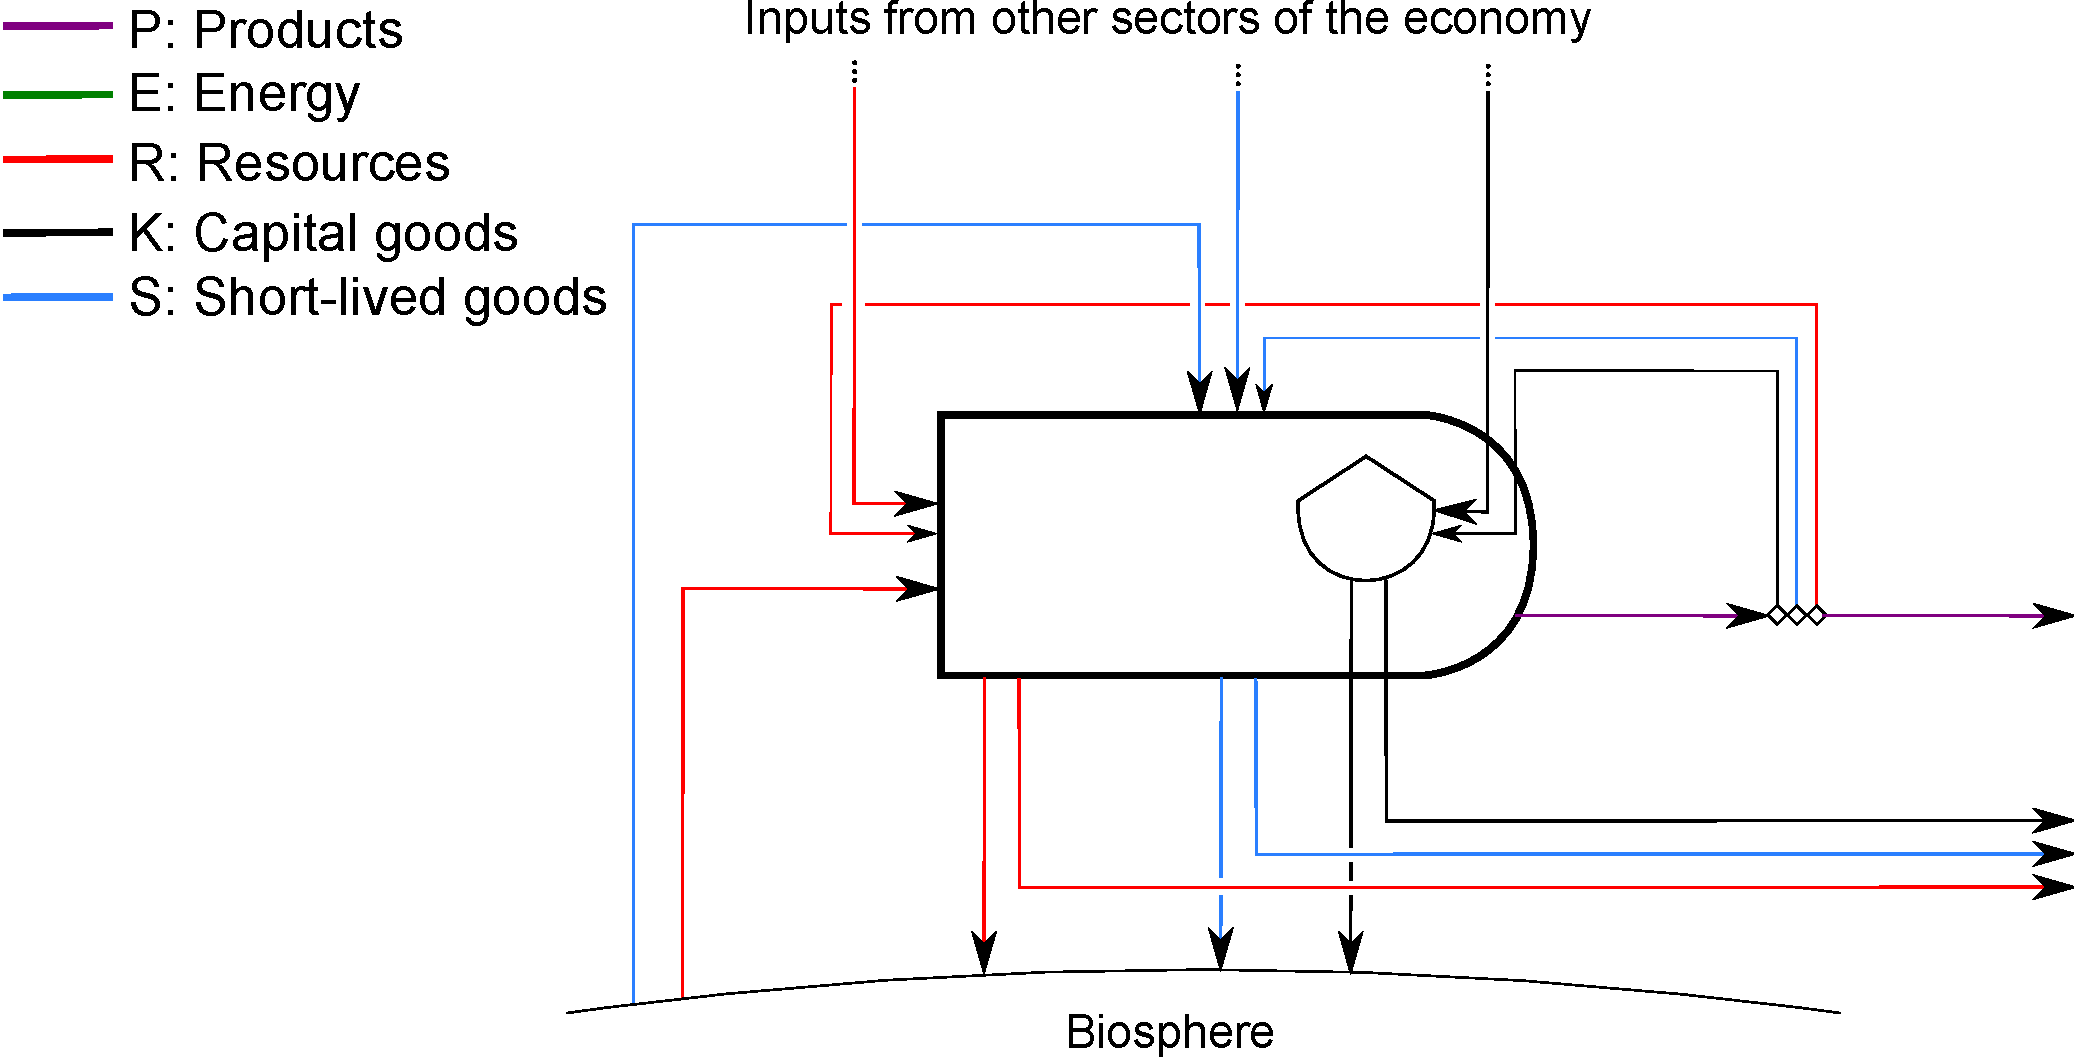
\includegraphics[width=\linewidth]{Part_3/Chapter_Unfinished/images/PERKS_basic_unit_materials_recycle.pdf}
	\caption[Material flows through an economic sector with waste treatment]{Material flows 
					through an economic sector with waste treatment flows to other economic sectors.}
\label{fig:PERKS_waste}
\end{figure}

Such flows violate the `one sector-one product' assumption of the Leontief inversion method.
Methods based on make-use tables,
as developed by von Neumann~\cite{vonNeumann1945} and Sraffa~\cite{Sraffa1960}
are able to account for multiple products from each sector.


%%%%%%%%%% People as capital stock %%%%%%%%%%
\section{Are people capital stock?}
\label{sec:people_as_stock}
%%%%%%%%%%

****

Mik: Suggest moving this discussion to the Materials chapter in the 
section that provides definitions,~\ref{sec:materials_definitions}.

****

There is an open
question as to what sort of \emph{stuff} 
should be included within the capital
that accumulates in society. 
Should the material constituting literal
\emph{human capital}---human bodies---be included? 
If humans are to be included within $K_{1}$, 
some resource flow~($\dot{R}_{i1}$)
must be converted into 
human capital flow~($\dot{K}_{11}$)
which then adds to the stock of human capital~($K_{1}$)
within society.
This resource flow is food.
Food itself represents a large ``resource''
flow and has a large associated energy content. 
Additionally, 
within industrial economies, 
a large amount of energy resources 
are channeled toward the production of food, 
meaning that the \emph{embodied energy}
of food may actually be several times larger than
the direct energy content of the food itself. 

Further questions arise. 
What is the ``product'' of society? 
A materialistic view might hold that the product of
society is human bodies and the labor they can accomplish. 
If so, 
should the agriculture industry 
be accounted as part of the energy sector 
because its aim is to provide 
an energy service (labor)? 
For non-industrial, agrarian societies, 
the proportion of total energy flow 
comprised by manual (or draft) energy 
may be large. 
In industrialized societies, 
it may be negligible, 
however, 
the energy flows necessary to support agriculture
may be many times larger than the food energy
(and certainly many times larger 
than the labor energy) 
delivered, therefore entailing an EROI of less than unity. 
Agrarian societies are necessarily constrained 
by the fact that the energy content of the food delivered 
\emph{must be} greater than the labor (and draft animal) 
energy required to produce it.

Another view is that societal capital~($K_{1}$) 
includes only man-made capital, 
i.e.\ items manufactured by humans,
but not humans themselves. 
For the purposes of the framework outlined in this book, 
we favored the latter view.
Other researchers favor the opposing view.\cite{Giampietro2013}
However,
the framework presented in this book is general enough to encompass either point of view.


%%%%%%%%%% The Sun %%%%%%%%%%
\section{What about the Sun?}
\label{sec:emergy}
%%%%%%%%%%

****

Matt: move to the very beginning of the Methodology
section of the Energy chapter, Section~\ref{sec:energy_methodology}.

Probably start by saying ``All energy comes from the sun.''
Then go on to the discussion below.

****

Costanza~\cite{Costanza:1978vd} included an option to consider 
solar energy as an input to the economy, 
thereby significantly increasing the energy intensity 
of agricultural sectors and other sectors 
that depend upon agricultural outputs. 
However later work by Costanza~\cite{Costanza:1984tq,Costanza:1980ww} 
did not include solar input to the economy.
Whether solar input to the economy 
should be considered in a materials, energy, and economic value 
accounting framework is probably dependent upon 
the objectives of the analysis. 

The motivation for this particular book is primarily 
the effects of declining energy resource quality
due to fossil fuel depletion on industrialized economies. 
As such, inclusion of solar flows is probably unnecessary. 
However, expanding the framework to include non-industrialized 
or agrarian societies may require accounting for solar energy flows. 

There are a number of means by which solar flows can be accounted. 
Solar energy flows could be accounted as short-term flows ($\dot{S}$)
for agricultural and forestry sectors, 
as well as 
solar thermal, 
solar photovoltaic, 
wind, 
ocean thermal, 
hydro, and
biomass
renewable energy
production sectors.
Doing so would not account for longer-term storage
of solar energy used to form fossil fuels, 
but fossil fuels are already accounted by the energy input vector ($\vec{E}_{0}$)
in the framework presented in this book.

A different approach that fully integrates solar 
into an energy framework is \emph{emergy} accounting.
The emergy method counts \emph{all} material flows 
in terms of \emph{em}bodied solar en\emph{ergy}.\cite{Odum1975, Odum1996}
The basic unit of measure is 
the \emph{em}joule which is often given in terms 
of flows of solar energy embodied in 
the energy (or material)---the solar emjoule---per unit of resource, 
abbreviated to seJ/J for energy resources, 
or seJ/kg for materials. 
As such, even fossil fuels, e.g.\ coal, 
extracted from the earth have an embodied energy 
of around 67,000~seJ/J.\cite{Brown2004} 


%%%%%%%%%% Endogenous %%%%%%%%%%
\section{What is endogenous?}
\label{sec:what_is_endogenous}
%%%%%%%%%%

****

Matt: Move to Energy Intensity chapter.

****

There is debate in the literature about whether government
and households
(Final Consumption~(1) in Figure~\ref{fig:B_materials}) 
should be endogenous to economic models.
This debate is a discussion about the appropriate analysis boundary.
Costanza~\cite{Costanza:1980ww} was the first to endogenize government and households, 
because households provide services to the economy (labor) in exchange for wages 
and government provides services to the economy in exchange for taxes, 
both of which require energy. 
Costanza~\cite{Costanza:1980ww} also demonstrated that 
energy intensity results
are a function of boundary (control volume) selection. 
By including government and households 
as sectors in the model, 
the variation of energy intensity is significantly reduced 
across all sectors of the economy. 

The key energy intensity equation in this book
(Equation~\ref{eq:epsilon_leontief_with_A})
was derived under the assumption that Final Consumption~(1)
is exogenous to energy intensity calculation.
However, Equation~\ref{eq:epsilon_leontief_with_A}
could be re-derived to endogenize 
Final Consumption~(1).

The total energy accounting equation for Final Consumption (1)
in Figure~\ref{fig:C_total_energy} can be written 
analogously to Equations~\ref{eq:C-Total_Energy_Sec_2-b}
and~\ref{eq:C-Total_Energy_Sec_3-b} as
%
\begin{equation} \label{eq:C-Total_Energy_Sec_1-unfinished}
	\frac{\mathrm{d}B_{K_{1}}}{\mathrm{d}t}
	= \dot{E}_{01}
	+ \varepsilon_{1} \dot{X}_{11}
	+ \varepsilon_{2} \dot{X}_{21}
	+ \varepsilon_{3} \dot{X}_{31}
	- \varepsilon_{1} \dot{X}_{1}
	- \left( \dot{B}_{\dot{R}_{10}} 
							+ \dot{B}_{\dot{S}_{10}}
							+ \gamma_{K,1} B_{K_{1}}
							\right).
\end{equation}
%
Furthermore, Equations~\ref{eq:C-Total_Energy_Sec_2-b}
and~\ref{eq:C-Total_Energy_Sec_3-b}
can be rewritten as 
%
\begin{equation} \label{eq:C-Total_Energy_Sec_2-unfinished}
	\frac{\mathrm{d}B_{K_{2}}}{\mathrm{d}t}
	= \dot{E}_{02}
	+ \varepsilon_{1} \dot{X}_{12}
	+ \varepsilon_{2} \dot{X}_{22}
	+ \varepsilon_{3} \dot{X}_{32}
	- \varepsilon_{2} \dot{X}_{2}
	- \left( \dot{B}_{\dot{R}_{20}} 
							+ \dot{B}_{\dot{S}_{20}}
							+ \gamma_{K,2} B_{K_{2}}
							\right)
\end{equation}
%
and
%
\begin{equation} \label{eq:C-Total_Energy_Sec_3-unfinished}
	\frac{\mathrm{d}B_{K_{3}}}{\mathrm{d}t}
	= \dot{E}_{03}
	+ \varepsilon_{1} \dot{X}_{13}
	+ \varepsilon_{2} \dot{X}_{23}
	+ \varepsilon_{3} \dot{X}_{33}
	- \varepsilon_{3} \dot{X}_{3}
	- \left( \dot{B}_{\dot{R}_{30}} 
							+ \dot{B}_{\dot{S}_{30}}
							+ \gamma_{K,3} B_{K_{3}}
							\right).
\end{equation}
%
Following the derivation of Chapter~\ref{chap:intensity},
we can obtain an updated version 
of Equation~\ref{eq:epsilon_leontief_with_A}:
%
\begin{equation} \label{eq:epsilon_leontief_depreciation_simplification_demand_endogenized}
	\boldsymbol{\varepsilon} 
	= {(\vec{I} - \vec{A}^{\mathrm{T}})}^{-1}\hat{\vec{X}}^{-1}
		\left[\vec{E}_{0} 
				- \frac{\mathrm{d}\vec{B}_{K}}{\mathrm{d}t} 
				- \vec{B}_{\dot{W}}
				- \hat{\boldsymbol{\gamma}}_{B}\vec{B}_{K}
		\right],
\end{equation}
%
wherein 
%
\begin{itemize}
	\item{the vectors and matrices of Equations~\ref{eq:B_vec_def}--\ref{eq:gamma_hat_matrix_def}
	and~\ref{eq:A_matrix_def} have been extended to include Final Consumption~(1) and}
	
	\item{Final Consumption~(1) has been endogenized
	(the $\vec{T}_{1}$ term of Equation~\ref{eq:epsilon_leontief_with_A}
	has been subsumed into the 
	${(\vec{I} - \vec{A}^{\mathrm{T}})}^{-1}\hat{\vec{X}}^{-1}$
	term of Equation~\ref{eq:epsilon_leontief_depreciation_simplification_demand_endogenized}).}
\end{itemize}

Future work could estimate energy intensity~($\boldsymbol{\varepsilon}$) 
using Equations~\ref{eq:epsilon_leontief_with_A}
and~\ref{eq:epsilon_leontief_depreciation_simplification_demand_endogenized}
with updated economic data for a wider range of countries.\footnote{Costanza's
analysis~\cite{Costanza:1980ww} was conducted using US data for 1963, 1967, and 1972.}
Doing so could provide further insight on Costanza's result~\cite{Costanza:1980ww}
that endogenizing Final Consumption (1) reduces variation 
of energy intensity across all sectors of the economy ($\boldsymbol{\varepsilon}$).


%%%%%%%%%% Unfinished: Summary %%%%%%%%%%
\section{Summary}
\label{sec:unfinished_summary}
%%%%%%%%%%

Any project with scope as large as this will, out of necessity, leave
several items undone.
This chapter reviewed our list of unfinished business.

Section~\ref{sec:theory_of_value} called for new approaches
to ascribe value to material flows between the economy and the biosphere.
Thereafter, we reviewed our call for better data collection and reporting
in Section~\ref{sec:Data}.

The remainder of this chapter discussed several questions
and methodological issues that arise from the framework
developed in this book.
Section~\ref{sec:hybrid} discussed opportunities to utilize hybrid EI-O and process methods
to estimate embodied energy and energy intensity.
Resource quality and co-products were discussed 
in Sections~\ref{sec:resource_quality_and_irreversibility}
and~\ref{sec:make-use}, respectively.
An extension to our accounting framework necessary to account
waste treatment and recycling was discussed in Section~\ref{sec:recycling_and_waste}.
Then, several questions were posed:
%
\begin{itemize}
	\item{are people capital stock?}
	
	\item{what about the Sun? and}
	
	\item{what is endogenous?}
\end{itemize}
%
In all of the above areas, we called for additional 
inquiry and research 
into the questions raised by our framework.

The following chapter summarizes the book. 


\bibliographystyle{unsrt}
\bibliography{../../Metabolic}


% Always give a unique label
% and use \ref{<label>} for cross-references
% and \cite{<label>} for bibliographic references
% use \sectionmark{}
% to alter or adjust the section heading in the running head
%% Instead of simply listing headings of different levels we recommend to let every heading be followed by at least a short passage of text. Furtheron please use the \LaTeX\ automatism for all your cross-references and citations.

%% Please note that the first line of text that follows a heading is not indented, whereas the first lines of all subsequent paragraphs are.

%% Use the standard \verb|equation| environment to typeset your equations, e.g.
%
%% \begin{equation}
%% a \times b = c\;,
%% \end{equation}
%
%% however, for multiline equations we recommend to use the \verb|eqnarray|
%% environment\footnote{In physics texts please activate the class option \texttt{vecphys} to depict your vectors in \textbf{\itshape boldface-italic} type - as is customary for a wide range of physical subjects.}.
%% \begin{eqnarray}
%% a \times b = c \nonumber\\
%% \vec{a} \cdot \vec{b}=\vec{c}
%% \label{eq:01}
%% \end{eqnarray}

%% \subsection{Subsection Heading}
%% \label{subsec:2}
%% Instead of simply listing headings of different levels we recommend to let every heading be followed by at least a short passage of text. Furtheron please use the \LaTeX\ automatism for all your cross-references\index{cross-references} and citations\index{citations} as has already been described in Sect.~\ref{sec:2}.

%% \begin{quotation}
%% Please do not use quotation marks when quoting texts! Simply use the \verb|quotation| environment -- it will automatically render Springer's preferred layout.
%% \end{quotation}


%% \subsubsection{Subsubsection Heading}
%% Instead of simply listing headings of different levels we recommend to let every heading be followed by at least a short passage of text. Furtheron please use the \LaTeX\ automatism for all your cross-references and citations as has already been described in Sect.~\ref{subsec:2}, see also Fig.~\ref{fig:1}\footnote{If you copy text passages, figures, or tables from other works, you must obtain \textit{permission} from the copyright holder (usually the original publisher). Please enclose the signed permission with the manucript. The sources\index{permission to print} must be acknowledged either in the captions, as footnotes or in a separate section of the book.}

%% Please note that the first line of text that follows a heading is not indented, whereas the first lines of all subsequent paragraphs are.

% For figures use
%
%% \begin{figure}[b]
%% \sidecaption
% Use the relevant command for your figure-insertion program
% to insert the figure file.
% For example, with the option graphics use
%% \includegraphics[scale=.65]{figure}
%
% If not, use
%\picplace{5cm}{2cm} % Give the correct figure height and width in cm
%
%% \caption{If the width of the figure is less than 7.8 cm use the \texttt{sidecapion} command to flush the caption on the left side of the page. If the figure is positioned at the top of the page, align the sidecaption with the top of the figure -- to achieve this you simply need to use the optional argument \texttt{[t]} with the \texttt{sidecaption} command}
%% \label{fig:1}       % Give a unique label
%% \end{figure}


%% \paragraph{Paragraph Heading} %
%% Instead of simply listing headings of different levels we recommend to let every heading be followed by at least a short passage of text. Furtheron please use the \LaTeX\ automatism for all your cross-references and citations as has already been described in Sect.~\ref{sec:2}.

%% Please note that the first line of text that follows a heading is not indented, whereas the first lines of all subsequent paragraphs are.

%% For typesetting numbered lists we recommend to use the \verb|enumerate| environment -- it will automatically render Springer's preferred layout.

%% \begin{enumerate}
%% \item{Livelihood and survival mobility are oftentimes coutcomes of uneven socioeconomic development.}
%% \begin{enumerate}
%% \item{Livelihood and survival mobility are oftentimes coutcomes of uneven socioeconomic development.}
%% \item{Livelihood and survival mobility are oftentimes coutcomes of uneven socioeconomic development.}
%% \end{enumerate}
%% \item{Livelihood and survival mobility are oftentimes coutcomes of uneven socioeconomic development.}
%% \end{enumerate}


%% \subparagraph{Subparagraph Heading} In order to avoid simply listing headings of different levels we recommend to let every heading be followed by at least a short passage of text. Use the \LaTeX\ automatism for all your cross-references and citations as has already been described in Sect.~\ref{sec:2}, see also Fig.~\ref{fig:2}.

%% Please note that the first line of text that follows a heading is not indented, whereas the first lines of all subsequent paragraphs are.

%% For unnumbered list we recommend to use the \verb|itemize| environment -- it will automatically render Springer's preferred layout.

%% \begin{itemize}
%% \item{Livelihood and survival mobility are oftentimes coutcomes of uneven socioeconomic development, cf. Table~\ref{tab:1}.}
%% \begin{itemize}
%% \item{Livelihood and survival mobility are oftentimes coutcomes of uneven socioeconomic development.}
%% \item{Livelihood and survival mobility are oftentimes coutcomes of uneven socioeconomic development.}
%% \end{itemize}
%% \item{Livelihood and survival mobility are oftentimes coutcomes of uneven socioeconomic development.}
%% \end{itemize}

%% \begin{figure}[t]
%% \sidecaption[t]
% Use the relevant command for your figure-insertion program
% to insert the figure file.
% For example, with the option graphics use
%% \includegraphics[scale=.65]{figure}
%
% If not, use
%\picplace{5cm}{2cm} % Give the correct figure height and width in cm
%
%% \caption{Please write your figure caption here}
%% \label{fig:2}       % Give a unique label
%% \end{figure}

%% \runinhead{Run-in Heading Boldface Version} Use the \LaTeX\ automatism for all your cross-references and citations as has already been described in Sect.~\ref{sec:2}.

%% \subruninhead{Run-in Heading Italic Version} Use the \LaTeX\ automatism for all your cross-refer\-ences and citations as has already been described in Sect.~\ref{sec:2}\index{paragraph}.
% Use the \index{} command to code your index words
%
% For tables use
%
%% \begin{table}
%% \caption{Please write your table caption here}
%% \label{tab:1}       % Give a unique label
%
% For LaTeX tables use
%
%% \begin{tabular}{p{2cm}p{2.4cm}p{2cm}p{4.9cm}}
%% \hline\noalign{\smallskip}
%% Classes & Subclass & Length & Action Mechanism  \\
%% \noalign{\smallskip}\svhline\noalign{\smallskip}
%% Translation & mRNA$^a$  & 22 (19--25) & Translation repression, mRNA cleavage\\
%% Translation & mRNA cleavage & 21 & mRNA cleavage\\
%% Translation & mRNA  & 21--22 & mRNA cleavage\\
%%Translation & mRNA  & 24--26 & Histone and DNA Modification\\
%%\noalign{\smallskip}\hline\noalign{\smallskip}
%%\end{tabular}
%%$^a$ Table foot note (with superscript)
%%\end{table}
%
%% \section{Section Heading}
%%\label{sec:3}
% Always give a unique label
% and use \ref{<label>} for cross-references
% and \cite{<label>} for bibliographic references
% use \sectionmark{}
% to alter or adjust the section heading in the running head
%% Instead of simply listing headings of different levels we recommend to let every heading be followed by at least a short passage of text. Furtheron please use the \LaTeX\ automatism for all your cross-references and citations as has already been described in Sect.~\ref{sec:2}.

%% Please note that the first line of text that follows a heading is not indented, whereas the first lines of all subsequent paragraphs are.

%%If you want to list definitions or the like we recommend to use the Springer-enhanced \verb|description| environment -- it will automatically render Springer's preferred layout.

%%\begin{description}[Type 1]
%%\item[Type 1]{That addresses central themes pertainng to migration, health, and disease. In Sect.~\ref{sec:1}, Wilson discusses the role of human migration in infectious disease distributions and patterns.}
%%\item[Type 2]{That addresses central themes pertainng to migration, health, and disease. In Sect.~\ref{subsec:2}, Wilson discusses the role of human migration in infectious disease distributions and patterns.}
%%\end{description}

%%\subsection{Subsection Heading} %
%% In order to avoid simply listing headings of different levels we recommend to let every heading be followed by at least a short passage of text. Use the \LaTeX\ automatism for all your cross-references and citations citations as has already been described in Sect.~\ref{sec:2}.

%% Please note that the first line of text that follows a heading is not indented, whereas the first lines of all subsequent paragraphs are.

%% \begin{svgraybox}
%% If you want to emphasize complete paragraphs of texts we recommend to use the newly defined Springer class option \verb|graybox| and the newly defined environment \verb|svgraybox|. This will produce a 15 percent screened box 'behind' your text.

%% If you want to emphasize complete paragraphs of texts we recommend to use the newly defined Springer class option and environment \verb|svgraybox|. This will produce a 15 percent screened box 'behind' your text.
%% \end{svgraybox}


%% \subsubsection{Subsubsection Heading}
%%Instead of simply listing headings of different levels we recommend to let every heading be followed by at least a short passage of text. Furtheron please use the \LaTeX\ automatism for all your cross-references and citations as has already been described in Sect.~\ref{sec:2}.

%% Please note that the first line of text that follows a heading is not indented, whereas the first lines of all subsequent paragraphs are.

%% \begin{theorem}
%% Theorem text goes here.
%% \end{theorem}
%
% or
%
%% \begin{definition}
%% Definition text goes here.
%% \end{definition}

%% \begin{proof}
%\smartqed
%% Proof text goes here.
%% \qed
%% \end{proof}

%%\paragraph{Paragraph Heading} %
%% Instead of simply listing headings of different levels we recommend to let every heading be followed by at least a short passage of text. Furtheron please use the \LaTeX\ automatism for all your cross-references and citations as has already been described in Sect.~\ref{sec:2}.

%% Note that the first line of text that follows a heading is not indented, whereas the first lines of all subsequent paragraphs are.
%
% For built-in environments use
%
%%\begin{theorem}
%%Theorem text goes here.
%%\end{theorem}
%
%%\begin{definition}
%%Definition text goes here.
%%\end{definition}
%
%%\begin{proof}
%%\smartqed
%% Proof text goes here.
%%\qed
%%\end{proof}
%
%% \begin{acknowledgement}
%% If you want to include acknowledgments of assistance and the like at the end of an individual chapter please use the \verb|acknowledgement| environment -- it will automatically render Springer's preferred layout.
%% \end{acknowledgement}
%
%% \section*{Appendix}
%% \addcontentsline{toc}{section}{Appendix}
%
%% When placed at the end of a chapter or contribution (as opposed to at the end of the book), the numbering of tables, figures, and equations in the appendix section continues on from that in the main text. Hence please \textit{do not} use the \verb|appendix| command when writing an appendix at the end of your chapter or contribution. If there is only one the appendix is designated ``Appendix'', or ``Appendix 1'', or ``Appendix 2'', etc. if there is more than one.

%% \begin{equation}
%% a \times b = c
%% \end{equation}
% Problems or Exercises should be sorted chapterwise
%% \section*{Problems}
%% \addcontentsline{toc}{section}{Problems}
%
% Use the following environment.
% Don't forget to label each problem;
% the label is needed for the solutions' environment
%% \begin{prob}
%% \label{prob1}
%% A given problem or Excercise is described here. The
%% problem is described here. The problem is described here.
%% \end{prob}

%% \begin{prob}
%% \label{prob2}
%% \textbf{Problem Heading}\\
%% (a) The first part of the problem is described here.\\
%% (b) The second part of the problem is described here.
%% \end{prob}




%!TEX root = ../../Heun_Dale_Haney_A_dynamic_approach_to_input_output_modeling.tex
%%%%%%%%%%%%%%%%%%%%% chapter.tex %%%%%%%%%%%%%%%%%%%%%%%%%%%%%%%%%
%
% sample chapter
%
% Use this file as a template for your own input.
%
%%%%%%%%%%%%%%%%%%%%%%%% Springer-Verlag %%%%%%%%%%%%%%%%%%%%%%%%%%
%\motto{Use the template \emph{chapter.tex} to style the various elements of your chapter content.}
\motto{Only a crisis---actual or perceived---produces real change. 
When that crisis occurs, the actions that are 
taken depend on the ideas that are lying around.~\emph{\cite[p.~ix]{Friedman:1982aa}}

\hfill---\emph{Milton Friedman}}


%%%%%%%%%%%%%%%%%%%%%%%%%%%%%
%%%%%%%%%% Summary %%%%%%%%%%
%%%%%%%%%%%%%%%%%%%%%%%%%%%%%
\chapter{Next steps}
% Always give a unique label
\label{chap:summary}
% use \chaptermark{} to alter or adjust the chapter heading in the running head
\chaptermark{Summary}
%%%%%%%%%%%%%%%%%%%%%%%%%%%%%%%%%%
%%%%%%%%%%%%%%%%%%%%%%%%%%%%%%%%%%
%%%%%%%%%%%%%%%%%%%%%%%%%%%%%%%%%%

%% \abstract{Each chapter should be preceded by an abstract (10--15 lines long) that summarizes the content. The abstract will appear \textit{online} at \url{www.SpringerLink.com} and be available with unrestricted access. This allows unregistered users to read the abstract as a teaser for the complete chapter. As a general rule the abstracts will not appear in the printed version of your book unless it is the style of your particular book or that of the series to which your book belongs.\newline\indent
%% Please use the 'starred' version of the new Springer \texttt{abstract} command for typesetting the text of the online abstracts (cf. source file of this chapter template \texttt{abstract}) and include them with the source files of your manuscript. Use the plain \texttt{abstract} command if the abstract is also to appear in the printed version of the book.}

%% Use the template \emph{chapter.tex} together with the Springer document class SVMono (monograph-type books) or SVMult (edited books) to style the various elements of your chapter content in the Springer layout.

\abstract*{This chapter briefly summarizes the book 
and highlights the need for additional data
on both inter-sector flows and accumulation 
of manufactured capital and associated embodied energy.
We continue with a call to action, 
a list containing several tasks that should be undertaken
to modify national accounting.
Finally, we note that moving forward on these issues
will be politically difficult, but necessary, 
to adapt to the age of resource depletion.}


We indicated at the outset (Chapters~\ref{chap:intro} and~\ref{chap:acct_for_won})
that this book would be about counting and change;
counting materials, counting energy, and counting economic value,
so that we can manage the upcoming energy transition
and navigate our way through the age of resource depletion.
Our motivation for counting more carefully
is mounting evidence (discussed in Chapter~\ref{chap:intro}) that 
scarcity of materials, energy, and 
assimilation capacity of the biosphere are impacting
capacity for continued economic growth in mature economies, 
thereby affecting us all.
We need to know precisely \emph{how} and \emph{at what rate} 
we are using our material and energy resources today
if we are to undertake the necessary transition to 
a more sustainable global economy.
But, before collecting such data,
we argued that we, as a society, 
need a rigorous theoretical framework for better systems of national accounts, 
one that goes beyond GDP and one that is relevant to the age of resource depletion.
This was the motivation for this book and the methodology we present.

To develop such an accounting framework 
guided by the metabolism metaphor,
in (Chapters~\ref{chap:materials}--\ref{chap:value})
we applied control volume and thermodynamic accounting equations 
to economies that are \emph{open} to their surroundings,
that is they are open to inflows and outflows of \emph{both}
materials and energy.
Similar equations are often applied to thermodynamic machines:
engines, refrigerators, heat pumps, and power plants.
Application of our framework shows that 
national accounting should gather and disseminate
a great deal of additional physical, material data on real economies.
We need balance sheets in addition to income statements!
We need accounting in physical units in addition to financial units.
Work to account such flows is starting to be
undertaken at the economy-wide level,
particularly within Europe.\cite{EUROSTAT2011}
This work needs to continue, 
but sub-economy, inter-sector material and energy 
accounts need to be developed, too.

The need for rigorous and accurate data
is all the more pressing in light of the need,
as demonstrated in Chapter~\ref{chap:intensity}, 
to track the accumulation 
of manufactured capital and associated embodied energy
within sectors of the economy.
There is a critical need for systematic
collection and public dissemination of such data 
by a centralized agency.
However,
as discussed in the Prologue, 
such accounting is currently non-existent in the US.
The BEA is expressly forbidden by congress 
to collect such data
after the first
Integrated Environmental-Economic System of Accounts (IEESA)
tables were published in 1994.

Remember what they taught you at Harvard Business School,
``you can't manage what you don't measure''.
We add our voices to those encouraging governments and 
institutions to collect high-quality data on material 
and energy stocks and flows.
As the world confronts significant challenges
in the age of resource depletion,
it will be impossible to make wise decisions about
which materials to use,
which energy sources to develop, and 
which products to incentivize
without such data.

To that end, we recommend pursuit of the next steps in the following list
as a matter of urgency.

**** Need Becky's review of this list. ****

\begin{enumerate}
	\item{National accounting agencies worldwide should seek and be given
			mandates to estimate and disseminate information on 
			the value of transactions that occur outside of the market.
			In the US, the Bureau for Economic Analysis (BEA) should seek authorization 
			to re-start the IEESA. 
			(See the Prologue.)
			Doing so will allow accounting for material and energy resources
			that are currently outside of the market.
			(See Sections~\ref{sec:energy-economy_coupling}
			and~\ref{sec:change_needed}.)}
	\item{National accounting agencies worldwide should develop and maintain 
			balance sheets of both nautral and manufactured capital 
			in addition to income statements.
			Doing so will allow countries to assess whether they are at risk of drawing down
			their wealth to produce today's income, 
			thereby jeopardizing future quality of life.
			(See the Prologue and Section~\ref{sec:wealth_nations}.)}
	\item{All stocks and inter-sector flows should be provided 
			in physical as well as financial units.
			At present, national accounting disseminates data in financial units,
			not physical units such as kilograms and kilojoules,
			thereby disguising the biphysical nature of the economy.
			Doing so will allow analysis of the true 
			\emph{biophysical} nature of the economy.}
	\item{In the US, the BEA should restart detailed 
			Capital, Labor, Energy, Material, and Services (KLEMS)
			reporting.
			**** Becky, provide a sentence or two on what has been lost.
			They used to report per-sector. 
			Now, only aggregate values are reported. 
			Perhaps something like
			``In the past, KLEMS data were estimated and disseminated by the BEA
			on a per-sector basis.
			However, today, only economy-wide aggregate values are provided.[reference 
			to BEA KLEMS here.]''
			****
			Doing so will provide detailed, sector-level information 
			on material and energy flows
			in financial units.}
	\item{The US BEA should expand KLEMS to include the origin of all flows.
			At the time when KLEMS provided sector-level detail, 
			only aggregated \emph{inflows} to a sector were reported;
			the origins of diasggregated inflows was not reported.
			Doing so will provide a better picture, in financial units,
			of the structure of materials and energy dependence among economic sectors.}
	\item{Additional detail should be provided for waste flows.
		 	**** Becky, please review and revise. 
			Perhaps we can say something like
			``At present, aggregated flows into the waste sector are reported in financial units. 
			However, the origin of these flows is not reported.'' ****
			Doing so will allow for analyses of opportunities for recycling and re-use
			within economies.
			(See Sections~\ref{sec:autophagy} and \ref{sec:recycling}.)}
	\item{All data on stocks and inter-sector flows should be reported by a single, 
			centralized agency
			in both financial and physical units.
			This will require synchronizing and reconciling data that is now reported
			by several different organizations. 
			In the US, for example, the Energy Information Agency~(EIA) and the BEA
			should combine their respective energy data.
			The Environmental Protection Agency~(EPA) and the BEA 
			should combine their respective waste data.
			Perhaps more than any other change, 
			reporting in both physical and financial units 
			would highlight the interconnectedness
			of the economy and the biosphere to the world at large.}
	\item{The US BEA should publish capital formation data that does not include
			intellectual property. 
			Doing so will avoid double-counting of capital stock.
			(See Section~**** the section that discusses IP as capital. ****)}
	\item{All of the above should be estimated and disseminated on an annual basis.
			**** Becky, please add a sentence here. Perhaps it would be something like
			``At present, the US BEA reports GDP and most financial flow information 
			annually.
			However, economy-wide KLEMS data are reported every five years.'' ****
			Doing so will allow for assessment of trends 
			in the material and energy structures of economies.}
\end{enumerate}

There should be no illusion that this agenda will be easy to pursue.
In many places, 
it will be politically difficult to undertake these changes.
But, if we, as a society, can begin collecting these data, 
perhaps we can begin to also utilize
the analytical tools, metrics, and knowledge
needed to go beyond GDP 
and make wise choices for the future.
We hope that this book makes a positive contribution in that direction.


\bibliographystyle{unsrt}
\bibliography{../../Metabolic}


% Always give a unique label
% and use \ref{<label>} for cross-references
% and \cite{<label>} for bibliographic references
% use \sectionmark{}
% to alter or adjust the section heading in the running head
%% Instead of simply listing headings of different levels we recommend to let every heading be followed by at least a short passage of text. Furtheron please use the \LaTeX\ automatism for all your cross-references and citations.

%% Please note that the first line of text that follows a heading is not indented, whereas the first lines of all subsequent paragraphs are.

%% Use the standard \verb|equation| environment to typeset your equations, e.g.
%
%% \begin{equation}
%% a \times b = c\;,
%% \end{equation}
%
%% however, for multiline equations we recommend to use the \verb|eqnarray|
%% environment\footnote{In physics texts please activate the class option \texttt{vecphys} to depict your vectors in \textbf{\itshape boldface-italic} type - as is customary for a wide range of physical subjects.}.
%% \begin{eqnarray}
%% a \times b = c \nonumber\\
%% \vec{a} \cdot \vec{b}=\vec{c}
%% \label{eq:01}
%% \end{eqnarray}

%% \subsection{Subsection Heading}
%% \label{subsec:2}
%% Instead of simply listing headings of different levels we recommend to let every heading be followed by at least a short passage of text. Furtheron please use the \LaTeX\ automatism for all your cross-references\index{cross-references} and citations\index{citations} as has already been described in Sect.~\ref{sec:2}.

%% \begin{quotation}
%% Please do not use quotation marks when quoting texts! Simply use the \verb|quotation| environment -- it will automatically render Springer's preferred layout.
%% \end{quotation}


%% \subsubsection{Subsubsection Heading}
%% Instead of simply listing headings of different levels we recommend to let every heading be followed by at least a short passage of text. Furtheron please use the \LaTeX\ automatism for all your cross-references and citations as has already been described in Sect.~\ref{subsec:2}, see also Fig.~\ref{fig:1}\footnote{If you copy text passages, figures, or tables from other works, you must obtain \textit{permission} from the copyright holder (usually the original publisher). Please enclose the signed permission with the manucript. The sources\index{permission to print} must be acknowledged either in the captions, as footnotes or in a separate section of the book.}

%% Please note that the first line of text that follows a heading is not indented, whereas the first lines of all subsequent paragraphs are.

% For figures use
%
%% \begin{figure}[b]
%% \sidecaption
% Use the relevant command for your figure-insertion program
% to insert the figure file.
% For example, with the option graphics use
%% \includegraphics[scale=.65]{figure}
%
% If not, use
%\picplace{5cm}{2cm} % Give the correct figure height and width in cm
%
%% \caption{If the width of the figure is less than 7.8 cm use the \texttt{sidecapion} command to flush the caption on the left side of the page. If the figure is positioned at the top of the page, align the sidecaption with the top of the figure -- to achieve this you simply need to use the optional argument \texttt{[t]} with the \texttt{sidecaption} command}
%% \label{fig:1}       % Give a unique label
%% \end{figure}


%% \paragraph{Paragraph Heading} %
%% Instead of simply listing headings of different levels we recommend to let every heading be followed by at least a short passage of text. Furtheron please use the \LaTeX\ automatism for all your cross-references and citations as has already been described in Sect.~\ref{sec:2}.

%% Please note that the first line of text that follows a heading is not indented, whereas the first lines of all subsequent paragraphs are.

%% For typesetting numbered lists we recommend to use the \verb|enumerate| environment -- it will automatically render Springer's preferred layout.

%% \begin{enumerate}
%% \item{Livelihood and survival mobility are oftentimes coutcomes of uneven socioeconomic development.}
%% \begin{enumerate}
%% \item{Livelihood and survival mobility are oftentimes coutcomes of uneven socioeconomic development.}
%% \item{Livelihood and survival mobility are oftentimes coutcomes of uneven socioeconomic development.}
%% \end{enumerate}
%% \item{Livelihood and survival mobility are oftentimes coutcomes of uneven socioeconomic development.}
%% \end{enumerate}


%% \subparagraph{Subparagraph Heading} In order to avoid simply listing headings of different levels we recommend to let every heading be followed by at least a short passage of text. Use the \LaTeX\ automatism for all your cross-references and citations as has already been described in Sect.~\ref{sec:2}, see also Fig.~\ref{fig:2}.

%% Please note that the first line of text that follows a heading is not indented, whereas the first lines of all subsequent paragraphs are.

%% For unnumbered list we recommend to use the \verb|itemize| environment -- it will automatically render Springer's preferred layout.

%% \begin{itemize}
%% \item{Livelihood and survival mobility are oftentimes coutcomes of uneven socioeconomic development, cf. Table~\ref{tab:1}.}
%% \begin{itemize}
%% \item{Livelihood and survival mobility are oftentimes coutcomes of uneven socioeconomic development.}
%% \item{Livelihood and survival mobility are oftentimes coutcomes of uneven socioeconomic development.}
%% \end{itemize}
%% \item{Livelihood and survival mobility are oftentimes coutcomes of uneven socioeconomic development.}
%% \end{itemize}

%% \begin{figure}[t]
%% \sidecaption[t]
% Use the relevant command for your figure-insertion program
% to insert the figure file.
% For example, with the option graphics use
%% \includegraphics[scale=.65]{figure}
%
% If not, use
%\picplace{5cm}{2cm} % Give the correct figure height and width in cm
%
%% \caption{Please write your figure caption here}
%% \label{fig:2}       % Give a unique label
%% \end{figure}

%% \runinhead{Run-in Heading Boldface Version} Use the \LaTeX\ automatism for all your cross-references and citations as has already been described in Sect.~\ref{sec:2}.

%% \subruninhead{Run-in Heading Italic Version} Use the \LaTeX\ automatism for all your cross-refer\-ences and citations as has already been described in Sect.~\ref{sec:2}\index{paragraph}.
% Use the \index{} command to code your index words
%
% For tables use
%
%% \begin{table}
%% \caption{Please write your table caption here}
%% \label{tab:1}       % Give a unique label
%
% For LaTeX tables use
%
%% \begin{tabular}{p{2cm}p{2.4cm}p{2cm}p{4.9cm}}
%% \hline\noalign{\smallskip}
%% Classes & Subclass & Length & Action Mechanism  \\
%% \noalign{\smallskip}\svhline\noalign{\smallskip}
%% Translation & mRNA$^a$  & 22 (19--25) & Translation repression, mRNA cleavage\\
%% Translation & mRNA cleavage & 21 & mRNA cleavage\\
%% Translation & mRNA  & 21--22 & mRNA cleavage\\
%%Translation & mRNA  & 24--26 & Histone and DNA Modification\\
%%\noalign{\smallskip}\hline\noalign{\smallskip}
%%\end{tabular}
%%$^a$ Table foot note (with superscript)
%%\end{table}
%
%% \section{Section Heading}
%%\label{sec:3}
% Always give a unique label
% and use \ref{<label>} for cross-references
% and \cite{<label>} for bibliographic references
% use \sectionmark{}
% to alter or adjust the section heading in the running head
%% Instead of simply listing headings of different levels we recommend to let every heading be followed by at least a short passage of text. Furtheron please use the \LaTeX\ automatism for all your cross-references and citations as has already been described in Sect.~\ref{sec:2}.

%% Please note that the first line of text that follows a heading is not indented, whereas the first lines of all subsequent paragraphs are.

%%If you want to list definitions or the like we recommend to use the Springer-enhanced \verb|description| environment -- it will automatically render Springer's preferred layout.

%%\begin{description}[Type 1]
%%\item[Type 1]{That addresses central themes pertainng to migration, health, and disease. In Sect.~\ref{sec:1}, Wilson discusses the role of human migration in infectious disease distributions and patterns.}
%%\item[Type 2]{That addresses central themes pertainng to migration, health, and disease. In Sect.~\ref{subsec:2}, Wilson discusses the role of human migration in infectious disease distributions and patterns.}
%%\end{description}

%%\subsection{Subsection Heading} %
%% In order to avoid simply listing headings of different levels we recommend to let every heading be followed by at least a short passage of text. Use the \LaTeX\ automatism for all your cross-references and citations citations as has already been described in Sect.~\ref{sec:2}.

%% Please note that the first line of text that follows a heading is not indented, whereas the first lines of all subsequent paragraphs are.

%% \begin{svgraybox}
%% If you want to emphasize complete paragraphs of texts we recommend to use the newly defined Springer class option \verb|graybox| and the newly defined environment \verb|svgraybox|. This will produce a 15 percent screened box 'behind' your text.

%% If you want to emphasize complete paragraphs of texts we recommend to use the newly defined Springer class option and environment \verb|svgraybox|. This will produce a 15 percent screened box 'behind' your text.
%% \end{svgraybox}


%% \subsubsection{Subsubsection Heading}
%%Instead of simply listing headings of different levels we recommend to let every heading be followed by at least a short passage of text. Furtheron please use the \LaTeX\ automatism for all your cross-references and citations as has already been described in Sect.~\ref{sec:2}.

%% Please note that the first line of text that follows a heading is not indented, whereas the first lines of all subsequent paragraphs are.

%% \begin{theorem}
%% Theorem text goes here.
%% \end{theorem}
%
% or
%
%% \begin{definition}
%% Definition text goes here.
%% \end{definition}

%% \begin{proof}
%\smartqed
%% Proof text goes here.
%% \qed
%% \end{proof}

%%\paragraph{Paragraph Heading} %
%% Instead of simply listing headings of different levels we recommend to let every heading be followed by at least a short passage of text. Furtheron please use the \LaTeX\ automatism for all your cross-references and citations as has already been described in Sect.~\ref{sec:2}.

%% Note that the first line of text that follows a heading is not indented, whereas the first lines of all subsequent paragraphs are.
%
% For built-in environments use
%
%%\begin{theorem}
%%Theorem text goes here.
%%\end{theorem}
%
%%\begin{definition}
%%Definition text goes here.
%%\end{definition}
%
%%\begin{proof}
%%\smartqed
%% Proof text goes here.
%%\qed
%%\end{proof}
%
%% \begin{acknowledgement}
%% If you want to include acknowledgments of assistance and the like at the end of an individual chapter please use the \verb|acknowledgement| environment -- it will automatically render Springer's preferred layout.
%% \end{acknowledgement}
%
%% \section*{Appendix}
%% \addcontentsline{toc}{section}{Appendix}
%
%% When placed at the end of a chapter or contribution (as opposed to at the end of the book), the numbering of tables, figures, and equations in the appendix section continues on from that in the main text. Hence please \textit{do not} use the \verb|appendix| command when writing an appendix at the end of your chapter or contribution. If there is only one the appendix is designated ``Appendix'', or ``Appendix 1'', or ``Appendix 2'', etc. if there is more than one.

%% \begin{equation}
%% a \times b = c
%% \end{equation}
% Problems or Exercises should be sorted chapterwise
%% \section*{Problems}
%% \addcontentsline{toc}{section}{Problems}
%
% Use the following environment.
% Don't forget to label each problem;
% the label is needed for the solutions' environment
%% \begin{prob}
%% \label{prob1}
%% A given problem or Excercise is described here. The
%% problem is described here. The problem is described here.
%% \end{prob}

%% \begin{prob}
%% \label{prob2}
%% \textbf{Problem Heading}\\
%% (a) The first part of the problem is described here.\\
%% (b) The second part of the problem is described here.
%% \end{prob}




%!TEX root = ../../Heun_Dale_Haney_A_dynamic_approach_to_input_output_modeling.tex

% This page contains the Wendell Berry quote

\chapter*{}
\chaptermark{}

\thispagestyle{empty} % Removes the page number from this page.

\vspace*{50 mm}

\small{}

\begin{quote}
	If we apply our minds directly and competently to the needs of the earth, 
	then we will have begun to make fundamental and necessary changes in our minds. 
	We will begin to understand and to mistrust and to change our wasteful economy, 
	which markets not just the produce of the earth, 
	but also the earth's ability to produce. 
	We will see that beauty and utility are alike dependent upon the health of the world. 
	But we will also see through the fads and the fashions of protest. 
	We will see that war and oppression and pollution are not separate issues, 
	but are aspects of the same issue. 
	Amid the outcries for the liberation of this group or that, 
	we will know that no person is free except in the freedom of other persons, 
	and that man's only real freedom 
	is to know and faithfully occupy his place---a much humbler place 
	than we have been taught to think---in the order of creation.

	\hfill---Wendell Berry. 2002. \emph{The Art of the Commonplace: The Agrarian Essays.}
	Counterpoint, Berkely, California, p.~89.
\end{quote}


\normalsize{}


% \appendix

\begin{appendices}
	
	%!TEX root = ../Heun_Dale_Haney_A_dynamic_approach_to_input_output_modeling.tex
%%%%%%%%%%%%%%%%%%%%% chapter.tex %%%%%%%%%%%%%%%%%%%%%%%%%%%%%%%%%
%
% sample chapter
%
% Use this file as a template for your own input.
%
%%%%%%%%%%%%%%%%%%%%%%%% Springer-Verlag %%%%%%%%%%%%%%%%%%%%%%%%%%
%\motto{Use the template \emph{chapter.tex} to style the various elements of your chapter content.}
\chapter{Value flows for the US auto industry}
% Always give a unique label
\label{chap:auto_value_flows} 
% use \chaptermark{} to alter or adjust the chapter heading in the running head
\chaptermark{Auto value flows}


This appendix describes the calculations used 
to estimate the value flows to and from the US Auto Industry  
in Chapter~\ref{chap:value}.  
The details of the calculations and assumptions made to calculate 
each of the value flows is described in Table~\ref{tab:calculations}. 
The data sources are are described in Table~\ref{tab:data_definitions}. 
These data are free and available for download 
from the BEA website.
(See references in Table~\ref{tab:data_definitions}.)

\begin{table}[H]
\caption[Data sources and calculations for auto industry example]{Data sources and calculations for auto industry (IOC 3361MV) example.}
\begin{center}
  \begin{tabular}{l r @{\hspace{2em}} p{7cm}}
   \toprule 
                    & 2011 USD      &   \\ 
Value Flow          & (millions)    & Data Calculations \\
	\midrule
Resources           & \$175,491     &    2011 KLEMS Total Material Intermediate Inputs 
	into Auto Industry (IOC 3361MV). 
	Total Material Inputs (\$346,882), less self-use (\$139,259) 
	and inputs recategorized as services (\$32,132).\tablefootnote{Two commodities 
		categorized in the KLEMS data as ``Material'' intermediate inputs
		are ``Wholesale Trade'' (IOC 4200, \$26,580) and ``Truck Transportation.'' 
		(IOC 4840, \$5,552). 
		For our calculations, these commodities were recategorized as ``Services.''
		The value of the flows in the table reflects the fact that 
		these dollar amounts were subtracted from this ``Resource''
		flow and added to ``Short-lived Goods.''\label{fn:a}} 
	Self-use Resources are defined as the two intermediate commodity inputs: 
	Motor Vehicles, Bodies, Trailers \& Parts (IOC 3361, \$138,077), 
	and Motor Vehicles (IOC 336A, \$1,182). \\
&&\\
Energy              &   3,637       &    2011 KLEMS Total Energy Intermediate Inputs 
	into Auto Industry. 
	The sum of the value of all ``Energy'' intermediate inputs.               \\
	&&\\
Short-lived Goods   &   74,578      &   2011 KLEMS Total Service Intermediate Inputs 
	into Auto Industry.
	Total Inputs from Service Sector (\$42,446) 
	plus Wholesale Trade and Truck Transportation from the KLEMS Material
	category.\footref{fn:a}
	The value of waste services that are part of this value flow 
	is the sum of Water \& Sewage (IOC 2213, \$123) 
	and Waste Management Services (IOC 5620, \$381).    \\
&&\\
Capital             &  15,447      &   2011  Fixed Assets (non-residential detailed estimates).
	The total amount of Capital Investment by the Auto Industry (\$61,260) 
	less the purchase of capital made within the Auto Industry (\$15,181, see calculation for
	Capital (self-use) below).     \\  
 
&&\\
Gross Economic Output & 482,269     &   2011 Input-Output accounts. 
	The Use of Commodities by Industries before Redefinitions. 
	(Producers' Prices). 
	Total Industry Output for Industry 3361MV\@.
	Data downloaded from the Bea.gov website for the Automobile Industry (IOC 3361MV).  \\ 
&&\\
Resources (self-use) & 133,961      & 2011 Input-Output accounts. 
Self-Use of Resources that were made in the automobile industry (IOC 3361MV used by IOC 3361MV, \$133,961). \\
&&\\
Capital (self-use) &  15,181    & 2011  Fixed Assets (non-residential detailed estimates).
	Fixed Assets that appear to be
	capital made from within the Automobile Industry: 
	Autos, Internal combustion engines, Light trucks (including utility vehicles), 
	Other trucks, buses and truck trailers, 
	Custom software, \& Own account software.\tablefootnote{To confirm 
		that these fixed asset types (particularly ``Custom Software'' and 
		``Own account software'') actually originated from the Auto Industry 
		(that is, that they are truly self-made capital), 
		the I-O ``Make'' table was consulted to ensure 
		that these commodities were made by the Auto Industry.}      \\
&&\\  
Net Economic Output & 333,127   &   2011 Input-Output accounts. 
	The Use of Commodities by Industries before Redefinitions. 
	(Producers' Prices). Total Industry Output, less Self-Use of Capital 
	(\$15,181, calculated above) and less Self-Use of Resources 
	(IOC 3361MV used by IOC 3361MV, \$133,961).\tablefootnote{Note that 
		this self-use of resources is slightly lower than the one used 
		to calculate the total of self-use Resources (\$139,259) 
		that was subtracted from total Material inputs to arrive at a figure 
		for Resources from all other sectors (above). 
		This is because the KLEMS data, like the Fixed Asset data, 
		are more detailed than the standard I-O accounts 
		and may contain judgments and trend estimates.  
		For example, in 2011, the KLEMS total intermediate inputs 
		to the auto industry is higher than the amount 
		from the Use table: \$392,965 vs.\$368,476.}  \\
    \bottomrule
  \end{tabular}
\end{center}

\label{tab:calculations}
\end{table}


\begin{table}
\caption[BEA data sources]{BEA data sources.}
\begin{center}
  \begin{tabular}{l @{\hspace{2em}} p{10cm}}
   \toprule 
    Dataset & Details  \\ 

	\midrule
Use Tables & Annual Input-Output accounts. 
	These are the primary industry data collected by the BEA\@.
	The Use tables present what industries use what commodities 
	as intermediate goods, and the value of the commodities that end up as final goods. 
	The values are computed at Producer’s prices. 
	That is, the value includes the sales price, plus sales and excise taxes, 
	less any subsidies. 
	This table provides a link from Industry data to National data. 
	The sum of all final output is a measure of National GDP\@.
	An introduction to these data is available.\cite{Streitwieser:2011aa}
	The tables can be found online.\cite{BEAIOData}\\
 &\\

KLEMS & (K-capital, L-labor, E-energy, M-materials, and S-purchased services) 
	refers to broad categories of intermediate inputs 
	that are consumed by industries in their production 
	of goods and services.\cite{Strassner:2005aa}
	The detailed estimates of intermediate inputs of an industry 
	are classified into one of three cost categories:
	energy~(E), materials~(M), and purchased services~(S).
	The labor cost category~(L) includes an industry’s compensation to labor from value added, 
	and the capital cost category~(K) includes the industry’s 
	gross operating surplus plus taxes on production and imports less subsidies.  
	


	Important note: As of January 2014, the 1998--2011 KLEMS tables
	that were used for the analyses in Chapter~\ref{chap:value}) are 
	no longer available online. They have been archived and replaced 
	with the 2005-2012 revised format KLEMS dataset. Due to budget
	cuts, the new
	KLEMS only contains the Energy, Materials, and Service
	value flow \emph{totals}. It no longer captures the underlying detail
	sources. Thus, the authors' calculations for self-use of
	materials, and re-categorization of some material inputs
	to service inputs are not possible with the revised data.
	The original dataset used for these analyses are available
	by request from the BEA. For more information
	on the KLEMS revison, see \cite{kim2014}, \cite{BEAKLEMSData}.



	The authors hope, of course, that a reinviorated focus on
	the importance of these details for national accounting
	will provide justification for the BEA to return to 
	making publicly available the underyling detailed KLEMS data.\\
 & \\
Fixed Assets &  Fixed Assets Table. Detailed Fixed Assets Table. 
	Categorizes capital investment by industry into three categories:
	equipment, structure, and software. 
	To obtain an estimate of self-use of capital, 
	we went to the more detailed tables, 
	which are less reliable than the standard tables. 
	The BEA notes on the detailed tables indicates that 
	``the more detailed estimates are more likely to be based on judgmental trends, 
	on trends in the higher level aggregate, 
	or on less reliable source data.''~\cite[Table~2.5]{BEADetailedData}\\
    \bottomrule
  \end{tabular}

\end{center}
\label{tab:data_definitions}
\end{table}

% Footnotes that belong with Table \ref{tab:calculations}:
% 
% 
% \footnotesize{a. Two commodities categorized in the KLEMS data as ``Material'' intermediate inputs
%  are ``Wholesale Trade'' (IOC 4200, \$26,580) and ``Truck Transportation.'' (IOC 4840, \$5,552). 
% For our calculations, these commodities were recategorized as ``Services.''
% The value of the flows in the table reflects the fact that 
% these dollar amounts were subtracted from this ``Resource''
% flow and added to ``Short-lived Goods.''}
% 
% 
% 
% \footnotesize{b. To confirm that these fixed asset types (particularly ``Custom Software'' and ``Own account software'')
%  actually originated from the Auto Industry (that is, that they are truly self-made capital), the I-O ``Make'' table was consulted to ensure 
% that these commodities were made by the Auto Industry.}
% 
% 
% 
% \footnotesize{c. Note that this self-use of resources is slightly lower than the one used to calculate the total of self-use Resources (\$139,259) that was subtracted from total Material inputs to arrive at a figure for Resources from all other sectors (above). This is because the KLEMS data, like the Fixed Asset data, are more detailed than the standard I-O accounts and may contain judgments and trend estimates.  For example, in 2011, the KLEMS total intermediate inputs to the auto industry is higher than the amount from the Use table: \$392,965 vs.\$368,476.}

\clearpage{}

\bibliographystyle{unsrt}
\bibliography{../Metabolic}


% Always give a unique label
% and use \ref{<label>} for cross-references
% and \cite{<label>} for bibliographic references
% use \sectionmark{}
% to alter or adjust the section heading in the running head
%% Instead of simply listing headings of different levels we recommend to let every heading be followed by at least a short passage of text. Furtheron please use the \LaTeX\ automatism for all your cross-references and citations.

%% Please note that the first line of text that follows a heading is not indented, whereas the first lines of all sequent paragraphs are.

%% Use the standard \verb|equation| environment to typeset your equations, e.g.
%
%% \begin{equation}
%% a \times b = c\;,
%% \end{equation}
%
%% however, for multiline equations we recommend to use the \verb|eqnarray|
%% environment\footnote{In physics texts please activate the class option \texttt{vecphys} to depict your vectors in \textbf{\itshape boldface-italic} type - as is customary for a wide range of physical jects.}.
%% \begin{eqnarray}
%% a \times b = c \nonumber\\
%% \vec{a} \cdot \vec{b}=\vec{c}
%% \label{eq:01}
%% \end{eqnarray}

%% \section{section Heading}
%% \label{sec:2}
%% Instead of simply listing headings of different levels we recommend to let every heading be followed by at least a short passage of text. Furtheron please use the \LaTeX\ automatism for all your cross-references\index{cross-references} and citations\index{citations} as has already been described in Sect.~\ref{sec:2}.

%% \begin{quotation}
%% Please do not use quotation marks when quoting texts! Simply use the \verb|quotation| environment -- it will automatically render Springer's preferred layout.
%% \end{quotation}


%% \section{section Heading}
%% Instead of simply listing headings of different levels we recommend to let every heading be followed by at least a short passage of text. Furtheron please use the \LaTeX\ automatism for all your cross-references and citations as has already been described in Sect.~\ref{sec:2}, see also Fig.~\ref{fig:1}\footnote{If you copy text passages, figures, or tables from other works, you must obtain \textit{permission} from the copyright holder (usually the original publisher). Please enclose the signed permission with the manucript. The sources\index{permission to print} must be acknowledged either in the captions, as footnotes or in a separate section of the book.}

%% Please note that the first line of text that follows a heading is not indented, whereas the first lines of all sequent paragraphs are.

% For figures use
%
%% \begin{figure}[b]
%% \sidecaption
% Use the relevant command for your figure-insertion program
% to insert the figure file.
% For example, with the option graphics use
%% \includegraphics[scale=.65]{figure}
%
% If not, use
%\picplace{5cm}{2cm} % Give the correct figure height and width in cm
%
%% \caption{If the width of the figure is less than 7.8 cm use the \texttt{sidecapion} command to flush the caption on the left side of the page. If the figure is positioned at the top of the page, align the sidecaption with the top of the figure -- to achieve this you simply need to use the optional argument \texttt{[t]} with the \texttt{sidecaption} command}
%% \label{fig:1}       % Give a unique label
%% \end{figure}


%% \paragraph{Paragraph Heading} %
%% Instead of simply listing headings of different levels we recommend to let every heading be followed by at least a short passage of text. Furtheron please use the \LaTeX\ automatism for all your cross-references and citations as has already been described in Sect.~\ref{sec:2}.

%% Please note that the first line of text that follows a heading is not indented, whereas the first lines of all sequent paragraphs are.

%% For typesetting numbered lists we recommend to use the \verb|enumerate| environment -- it will automatically render Springer's preferred layout.

%% \begin{enumerate}
%% \item{Livelihood and survival mobility are oftentimes coutcomes of uneven socioeconomic development.}
%% \begin{enumerate}
%% \item{Livelihood and survival mobility are oftentimes coutcomes of uneven socioeconomic development.}
%% \item{Livelihood and survival mobility are oftentimes coutcomes of uneven socioeconomic development.}
%% \end{enumerate}
%% \item{Livelihood and survival mobility are oftentimes coutcomes of uneven socioeconomic development.}
%% \end{enumerate}


%% \paragraph{paragraph Heading} In order to avoid simply listing headings of different levels we recommend to let every heading be followed by at least a short passage of text. Use the \LaTeX\ automatism for all your cross-references and citations as has already been described in Sect.~\ref{sec:2}, see also Fig.~\ref{fig:2}.

%% Please note that the first line of text that follows a heading is not indented, whereas the first lines of all sequent paragraphs are.

%% For unnumbered list we recommend to use the \verb|itemize| environment -- it will automatically render Springer's preferred layout.

%% \begin{itemize}
%% \item{Livelihood and survival mobility are oftentimes coutcomes of uneven socioeconomic development, cf. Table~\ref{tab:1}.}
%% \begin{itemize}
%% \item{Livelihood and survival mobility are oftentimes coutcomes of uneven socioeconomic development.}
%% \item{Livelihood and survival mobility are oftentimes coutcomes of uneven socioeconomic development.}
%% \end{itemize}
%% \item{Livelihood and survival mobility are oftentimes coutcomes of uneven socioeconomic development.}
%% \end{itemize}

%% \begin{figure}[t]
%% \sidecaption[t]
% Use the relevant command for your figure-insertion program
% to insert the figure file.
% For example, with the option graphics use
%% \includegraphics[scale=.65]{figure}
%
% If not, use
%\picplace{5cm}{2cm} % Give the correct figure height and width in cm
%
%% \caption{Please write your figure caption here}
%% \label{fig:2}       % Give a unique label
%% \end{figure}

%% \runinhead{Run-in Heading Boldface Version} Use the \LaTeX\ automatism for all your cross-references and citations as has already been described in Sect.~\ref{sec:2}.

%% \runinhead{Run-in Heading Italic Version} Use the \LaTeX\ automatism for all your cross-refer\-ences and citations as has already been described in Sect.~\ref{sec:2}\index{paragraph}.
% Use the \index{} command to code your index words
%
% For tables use
%
%% \begin{table}
%% \caption{Please write your table caption here}
%% \label{tab:1}       % Give a unique label
%
% For LaTeX tables use
%
%% \begin{tabular}{p{2cm}p{2.4cm}p{2cm}p{4.9cm}}
%% \hline\noalign{\smallskip}
%% Classes & class & Length & Action Mechanism  \\
%% \noalign{\smallskip}\svhline\noalign{\smallskip}
%% Translation & mRNA$^a$  & 22 (19--25) & Translation repression, mRNA cleavage\\
%% Translation & mRNA cleavage & 21 & mRNA cleavage\\
%% Translation & mRNA  & 21--22 & mRNA cleavage\\
%%Translation & mRNA  & 24--26 & Histone and DNA Modification\\
%%\noalign{\smallskip}\hline\noalign{\smallskip}
%%\end{tabular}
%%$^a$ Table foot note (with superscript)
%%\end{table}
%
%% \section{Section Heading}
%%\label{sec:3}
% Always give a unique label
% and use \ref{<label>} for cross-references
% and \cite{<label>} for bibliographic references
% use \sectionmark{}
% to alter or adjust the section heading in the running head
%% Instead of simply listing headings of different levels we recommend to let every heading be followed by at least a short passage of text. Furtheron please use the \LaTeX\ automatism for all your cross-references and citations as has already been described in Sect.~\ref{sec:2}.

%% Please note that the first line of text that follows a heading is not indented, whereas the first lines of all sequent paragraphs are.

%%If you want to list definitions or the like we recommend to use the Springer-enhanced \verb|description| environment -- it will automatically render Springer's preferred layout.

%%\begin{description}[Type 1]
%%\item[Type 1]{That addresses central themes pertainng to migration, health, and disease. In Sect.~\ref{sec:1}, Wilson discusses the role of human migration in infectious disease distributions and patterns.}
%%\item[Type 2]{That addresses central themes pertainng to migration, health, and disease. In Sect.~\ref{sec:2}, Wilson discusses the role of human migration in infectious disease distributions and patterns.}
%%\end{description}

%%\section{section Heading} %
%% In order to avoid simply listing headings of different levels we recommend to let every heading be followed by at least a short passage of text. Use the \LaTeX\ automatism for all your cross-references and citations citations as has already been described in Sect.~\ref{sec:2}.

%% Please note that the first line of text that follows a heading is not indented, whereas the first lines of all sequent paragraphs are.

%% \begin{svgraybox}
%% If you want to emphasize complete paragraphs of texts we recommend to use the newly defined Springer class option \verb|graybox| and the newly defined environment \verb|svgraybox|. This will produce a 15 percent screened box 'behind' your text.

%% If you want to emphasize complete paragraphs of texts we recommend to use the newly defined Springer class option and environment \verb|svgraybox|. This will produce a 15 percent screened box 'behind' your text.
%% \end{svgraybox}


%% \section{section Heading}
%%Instead of simply listing headings of different levels we recommend to let every heading be followed by at least a short passage of text. Furtheron please use the \LaTeX\ automatism for all your cross-references and citations as has already been described in Sect.~\ref{sec:2}.

%% Please note that the first line of text that follows a heading is not indented, whereas the first lines of all sequent paragraphs are.

%% \begin{theorem}
%% Theorem text goes here.
%% \end{theorem}
%
% or
%
%% \begin{definition}
%% Definition text goes here.
%% \end{definition}

%% \begin{proof}
%\smartqed
%% Proof text goes here.
%% \qed
%% \end{proof}

%%\paragraph{Paragraph Heading} %
%% Instead of simply listing headings of different levels we recommend to let every heading be followed by at least a short passage of text. Furtheron please use the \LaTeX\ automatism for all your cross-references and citations as has already been described in Sect.~\ref{sec:2}.

%% Note that the first line of text that follows a heading is not indented, whereas the first lines of all subsequent paragraphs are.
%
% For built-in environments use
%
%%\begin{theorem}
%%Theorem text goes here.
%%\end{theorem}
%
%%\begin{definition}
%%Definition text goes here.
%%\end{definition}
%
%%\begin{proof}
%%\smartqed
%% Proof text goes here.
%%\qed
%%\end{proof}
%
%% \begin{acknowledgement}
%% If you want to include acknowledgments of assistance and the like at the end of an individual chapter please use the \verb|acknowledgement| environment -- it will automatically render Springer's preferred layout.
%% \end{acknowledgement}
%
%% \section*{Appendix}
%% \addcontentsline{toc}{section}{Appendix}
%
%% When placed at the end of a chapter or contribution (as opposed to at the end of the book), the numbering of tables, figures, and equations in the appendix section continues on from that in the main text. Hence please \textit{do not} use the \verb|appendix| command when writing an appendix at the end of your chapter or contribution. If there is only one the appendix is designated ``Appendix'', or ``Appendix 1'', or ``Appendix 2'', etc. if there is more than one.

%% \begin{equation}
%% a \times b = c
%% \end{equation}
% Problems or Exercises should be sorted chapterwise
%% \section*{Problems}
%% \addcontentsline{toc}{section}{Problems}
%
% Use the following environment.
% Don't forget to label each problem;
% the label is needed for the solutions' environment
%% \begin{prob}
%% \label{prob1}
%% A given problem or Excercise is described here. The
%% problem is described here. The problem is described here.
%% \end{prob}

%% \begin{prob}
%% \label{prob2}
%% \textbf{Problem Heading}\\
%% (a) The first part of the problem is described here.\\
%% (b) The second part of the problem is described here.
%% \end{prob}




	%!TEX root = ../Heun_Dale_Haney_A_dynamic_approach_to_input_output_modeling.tex
%%%%%%%%%%%%%%%%%%%%% chapter.tex %%%%%%%%%%%%%%%%%%%%%%%%%%%%%%%%%
%
% sample chapter
%
% Use this file as a template for your own input.
%
%%%%%%%%%%%%%%%%%%%%%%%% Springer-Verlag %%%%%%%%%%%%%%%%%%%%%%%%%%
%\motto{Use the template \emph{chapter.tex} to style the various elements of your chapter content.}
\chapter{Infinite series representation of energy intensity}
\label{chap:infinite_series} % Always give a unique label
% use \chaptermark{}
% to alter or adjust the chapter heading in the running head
\chaptermark{infinite series}

The single-sector economy 
of Figures~\ref{fig:A_materials},~\ref{fig:A_energy},~\ref{fig:A_total_energy_T_dot},
and~\ref{fig:A_value}
can be re-drawn as shown in Figure~\ref{fig:single_sector_flows_3}.

\begin{figure}[h!]
\centering\
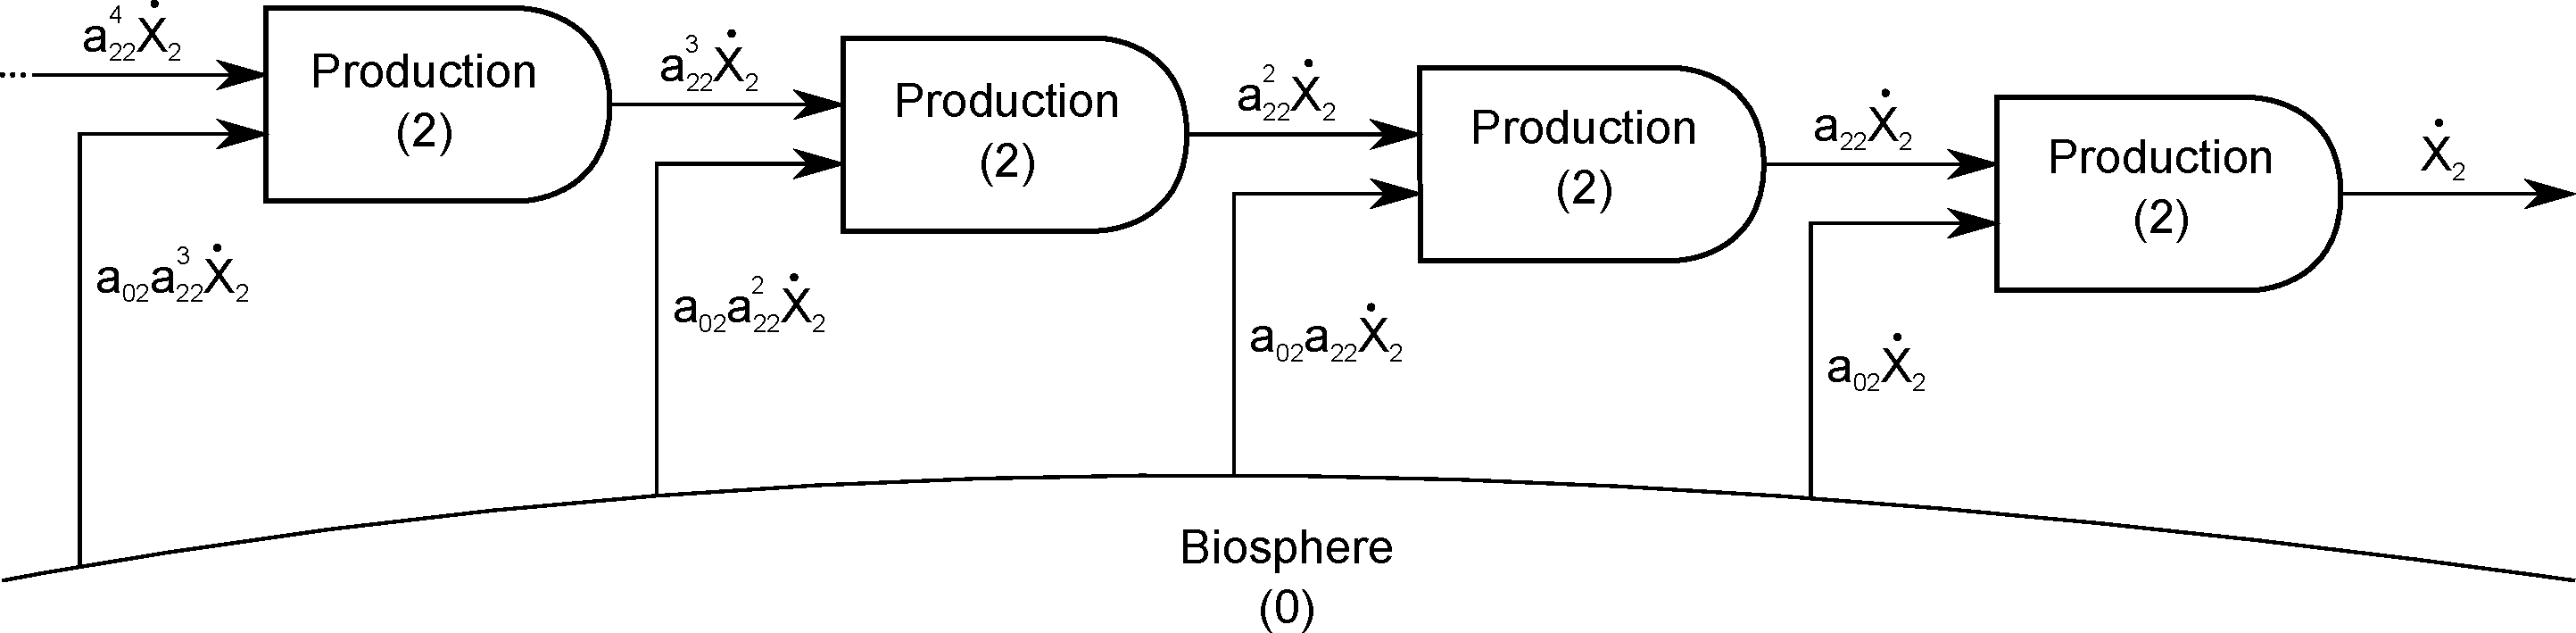
\includegraphics[width=1.0\linewidth]{Appendix_Infinite_Series/images/I-O_Process_Equivalence.pdf}
\caption{Process flows in a single-sector economy. ***** Mik: please update 
to include Biopshere (0), change ``Sector (2)'' to ``Production (1)'', 
and change all subscripts accordingly. ******}
\label{fig:single_sector_flows_3}
\end{figure}

The economy produces output at a rate of $\dot{X}_{1}$, 
but it requires energy from the biosphere 
($\dot{E}_{01} = a_{01}\dot{X}_{1}$) to do so. 
The economy also consumes a fraction 
of its own gross output 
($\dot{X}_{11} = a_{11}\dot{X}_{1}$). 
To produce $a_{11}\dot{X}_{1}$, 
the economy requires an additional $a_{01}a_{11}\dot{X}_{1}$ 
of energy from the biosphere. 
The sum of all direct energy ($\dot{E}$) required for the economy 
to produce at a rate of $\dot{X}_{1}$ is an infinite sum.

\begin{equation} \label{eq:E_dot_demand_SS}
	\dot{E}_{demand,tot} 
	= a_{01}\dot{X}_{1} 
	+ a_{01}a_{11}\dot{X}_{1} 
	+ a_{01}a_{11}^2\dot{X}_{1} 
	+ \ldots
\end{equation}

The energy intensity of the economy ($\varepsilon_{1}$) is 

\begin{equation} \label{eq:epsilon_process_SS_intermediate}
	\varepsilon_{1} 
	= \frac{\dot{E}_{demand,tot}}{\dot{X}_{1}} 
	= a_{01}(1 + a_{11} + a_{11}^2 + \ldots) 
	= a_{01}\sum_{n=0}^{\infty}a_{11}^{n}.
\end{equation}

Realizing that 
$\sum\limits_{n=0}^{\infty}a_{11}^{n} 
= \frac{1}{1-a_{11}}$ 
and 
$a_{01} 
= \frac{\dot{E}_{01}}{\dot{X}_{1}}$ 
(direct energy can be considered the output of the biosphere
in this situation) gives

\begin{equation} \label{eq:epsilon_process_SS}
	\varepsilon_{1} = {(1-a_{11})}^{-1} \dot{X}^{-1} \dot{E}_{01}.
\end{equation}

Neglecting 
accumulation of embodied energy in the economy
$\left( \frac{\mathrm{d}B_{1}}{\mathrm{d}t} = 0 \right)$
and depreciation $\left( \gamma_{1}B_{1} = 0 \right)$,
Equations~\ref{eq:eps3_ss_IO} and~\ref{eq:epsilon_process_SS} are identical, 
indicating that the I-O approach accounts 
for the infinite recursion of energy demand by the economy.
****** Fix this paragraph after editing Chapter 6. *****


\bibliographystyle{unsrt}
\bibliography{../../EROI_review_v2}


% Always give a unique label
% and use \ref{<label>} for cross-references
% and \cite{<label>} for bibliographic references
% use \sectionmark{}
% to alter or adjust the section heading in the running head
%% Instead of simply listing headings of different levels we recommend to let every heading be followed by at least a short passage of text. Furtheron please use the \LaTeX\ automatism for all your cross-references and citations.

%% Please note that the first line of text that follows a heading is not indented, whereas the first lines of all sequent paragraphs are.

%% Use the standard \verb|equation| environment to typeset your equations, e.g.
%
%% \begin{equation}
%% a \times b = c\;,
%% \end{equation}
%
%% however, for multiline equations we recommend to use the \verb|eqnarray|
%% environment\footnote{In physics texts please activate the class option \texttt{vecphys} to depict your vectors in \textbf{\itshape boldface-italic} type - as is customary for a wide range of physical jects.}.
%% \begin{eqnarray}
%% a \times b = c \nonumber\\
%% \vec{a} \cdot \vec{b}=\vec{c}
%% \label{eq:01}
%% \end{eqnarray}

%% \section{section Heading}
%% \label{sec:2}
%% Instead of simply listing headings of different levels we recommend to let every heading be followed by at least a short passage of text. Furtheron please use the \LaTeX\ automatism for all your cross-references\index{cross-references} and citations\index{citations} as has already been described in Sect.~\ref{sec:2}.

%% \begin{quotation}
%% Please do not use quotation marks when quoting texts! Simply use the \verb|quotation| environment -- it will automatically render Springer's preferred layout.
%% \end{quotation}


%% \section{section Heading}
%% Instead of simply listing headings of different levels we recommend to let every heading be followed by at least a short passage of text. Furtheron please use the \LaTeX\ automatism for all your cross-references and citations as has already been described in Sect.~\ref{sec:2}, see also Fig.~\ref{fig:1}\footnote{If you copy text passages, figures, or tables from other works, you must obtain \textit{permission} from the copyright holder (usually the original publisher). Please enclose the signed permission with the manucript. The sources\index{permission to print} must be acknowledged either in the captions, as footnotes or in a separate section of the book.}

%% Please note that the first line of text that follows a heading is not indented, whereas the first lines of all sequent paragraphs are.

% For figures use
%
%% \begin{figure}[b]
%% \sidecaption
% Use the relevant command for your figure-insertion program
% to insert the figure file.
% For example, with the option graphics use
%% \includegraphics[scale=.65]{figure}
%
% If not, use
%\picplace{5cm}{2cm} % Give the correct figure height and width in cm
%
%% \caption{If the width of the figure is less than 7.8 cm use the \texttt{sidecapion} command to flush the caption on the left side of the page. If the figure is positioned at the top of the page, align the sidecaption with the top of the figure -- to achieve this you simply need to use the optional argument \texttt{[t]} with the \texttt{sidecaption} command}
%% \label{fig:1}       % Give a unique label
%% \end{figure}


%% \paragraph{Paragraph Heading} %
%% Instead of simply listing headings of different levels we recommend to let every heading be followed by at least a short passage of text. Furtheron please use the \LaTeX\ automatism for all your cross-references and citations as has already been described in Sect.~\ref{sec:2}.

%% Please note that the first line of text that follows a heading is not indented, whereas the first lines of all sequent paragraphs are.

%% For typesetting numbered lists we recommend to use the \verb|enumerate| environment -- it will automatically render Springer's preferred layout.

%% \begin{enumerate}
%% \item{Livelihood and survival mobility are oftentimes coutcomes of uneven socioeconomic development.}
%% \begin{enumerate}
%% \item{Livelihood and survival mobility are oftentimes coutcomes of uneven socioeconomic development.}
%% \item{Livelihood and survival mobility are oftentimes coutcomes of uneven socioeconomic development.}
%% \end{enumerate}
%% \item{Livelihood and survival mobility are oftentimes coutcomes of uneven socioeconomic development.}
%% \end{enumerate}


%% \paragraph{paragraph Heading} In order to avoid simply listing headings of different levels we recommend to let every heading be followed by at least a short passage of text. Use the \LaTeX\ automatism for all your cross-references and citations as has already been described in Sect.~\ref{sec:2}, see also Fig.~\ref{fig:2}.

%% Please note that the first line of text that follows a heading is not indented, whereas the first lines of all sequent paragraphs are.

%% For unnumbered list we recommend to use the \verb|itemize| environment -- it will automatically render Springer's preferred layout.

%% \begin{itemize}
%% \item{Livelihood and survival mobility are oftentimes coutcomes of uneven socioeconomic development, cf. Table~\ref{tab:1}.}
%% \begin{itemize}
%% \item{Livelihood and survival mobility are oftentimes coutcomes of uneven socioeconomic development.}
%% \item{Livelihood and survival mobility are oftentimes coutcomes of uneven socioeconomic development.}
%% \end{itemize}
%% \item{Livelihood and survival mobility are oftentimes coutcomes of uneven socioeconomic development.}
%% \end{itemize}

%% \begin{figure}[t]
%% \sidecaption[t]
% Use the relevant command for your figure-insertion program
% to insert the figure file.
% For example, with the option graphics use
%% \includegraphics[scale=.65]{figure}
%
% If not, use
%\picplace{5cm}{2cm} % Give the correct figure height and width in cm
%
%% \caption{Please write your figure caption here}
%% \label{fig:2}       % Give a unique label
%% \end{figure}

%% \runinhead{Run-in Heading Boldface Version} Use the \LaTeX\ automatism for all your cross-references and citations as has already been described in Sect.~\ref{sec:2}.

%% \runinhead{Run-in Heading Italic Version} Use the \LaTeX\ automatism for all your cross-refer\-ences and citations as has already been described in Sect.~\ref{sec:2}\index{paragraph}.
% Use the \index{} command to code your index words
%
% For tables use
%
%% \begin{table}
%% \caption{Please write your table caption here}
%% \label{tab:1}       % Give a unique label
%
% For LaTeX tables use
%
%% \begin{tabular}{p{2cm}p{2.4cm}p{2cm}p{4.9cm}}
%% \hline\noalign{\smallskip}
%% Classes & class & Length & Action Mechanism  \\
%% \noalign{\smallskip}\svhline\noalign{\smallskip}
%% Translation & mRNA$^a$  & 22 (19--25) & Translation repression, mRNA cleavage\\
%% Translation & mRNA cleavage & 21 & mRNA cleavage\\
%% Translation & mRNA  & 21--22 & mRNA cleavage\\
%%Translation & mRNA  & 24--26 & Histone and DNA Modification\\
%%\noalign{\smallskip}\hline\noalign{\smallskip}
%%\end{tabular}
%%$^a$ Table foot note (with superscript)
%%\end{table}
%
%% \section{Section Heading}
%%\label{sec:3}
% Always give a unique label
% and use \ref{<label>} for cross-references
% and \cite{<label>} for bibliographic references
% use \sectionmark{}
% to alter or adjust the section heading in the running head
%% Instead of simply listing headings of different levels we recommend to let every heading be followed by at least a short passage of text. Furtheron please use the \LaTeX\ automatism for all your cross-references and citations as has already been described in Sect.~\ref{sec:2}.

%% Please note that the first line of text that follows a heading is not indented, whereas the first lines of all sequent paragraphs are.

%%If you want to list definitions or the like we recommend to use the Springer-enhanced \verb|description| environment -- it will automatically render Springer's preferred layout.

%%\begin{description}[Type 1]
%%\item[Type 1]{That addresses central themes pertainng to migration, health, and disease. In Sect.~\ref{sec:1}, Wilson discusses the role of human migration in infectious disease distributions and patterns.}
%%\item[Type 2]{That addresses central themes pertainng to migration, health, and disease. In Sect.~\ref{sec:2}, Wilson discusses the role of human migration in infectious disease distributions and patterns.}
%%\end{description}

%%\section{section Heading} %
%% In order to avoid simply listing headings of different levels we recommend to let every heading be followed by at least a short passage of text. Use the \LaTeX\ automatism for all your cross-references and citations citations as has already been described in Sect.~\ref{sec:2}.

%% Please note that the first line of text that follows a heading is not indented, whereas the first lines of all sequent paragraphs are.

%% \begin{svgraybox}
%% If you want to emphasize complete paragraphs of texts we recommend to use the newly defined Springer class option \verb|graybox| and the newly defined environment \verb|svgraybox|. This will produce a 15 percent screened box 'behind' your text.

%% If you want to emphasize complete paragraphs of texts we recommend to use the newly defined Springer class option and environment \verb|svgraybox|. This will produce a 15 percent screened box 'behind' your text.
%% \end{svgraybox}


%% \section{section Heading}
%%Instead of simply listing headings of different levels we recommend to let every heading be followed by at least a short passage of text. Furtheron please use the \LaTeX\ automatism for all your cross-references and citations as has already been described in Sect.~\ref{sec:2}.

%% Please note that the first line of text that follows a heading is not indented, whereas the first lines of all sequent paragraphs are.

%% \begin{theorem}
%% Theorem text goes here.
%% \end{theorem}
%
% or
%
%% \begin{definition}
%% Definition text goes here.
%% \end{definition}

%% \begin{proof}
%\smartqed
%% Proof text goes here.
%% \qed
%% \end{proof}

%%\paragraph{Paragraph Heading} %
%% Instead of simply listing headings of different levels we recommend to let every heading be followed by at least a short passage of text. Furtheron please use the \LaTeX\ automatism for all your cross-references and citations as has already been described in Sect.~\ref{sec:2}.

%% Note that the first line of text that follows a heading is not indented, whereas the first lines of all subsequent paragraphs are.
%
% For built-in environments use
%
%%\begin{theorem}
%%Theorem text goes here.
%%\end{theorem}
%
%%\begin{definition}
%%Definition text goes here.
%%\end{definition}
%
%%\begin{proof}
%%\smartqed
%% Proof text goes here.
%%\qed
%%\end{proof}
%
%% \begin{acknowledgement}
%% If you want to include acknowledgments of assistance and the like at the end of an individual chapter please use the \verb|acknowledgement| environment -- it will automatically render Springer's preferred layout.
%% \end{acknowledgement}
%
%% \section*{Appendix}
%% \addcontentsline{toc}{section}{Appendix}
%
%% When placed at the end of a chapter or contribution (as opposed to at the end of the book), the numbering of tables, figures, and equations in the appendix section continues on from that in the main text. Hence please \textit{do not} use the \verb|appendix| command when writing an appendix at the end of your chapter or contribution. If there is only one the appendix is designated ``Appendix'', or ``Appendix 1'', or ``Appendix 2'', etc. if there is more than one.

%% \begin{equation}
%% a \times b = c
%% \end{equation}
% Problems or Exercises should be sorted chapterwise
%% \section*{Problems}
%% \addcontentsline{toc}{section}{Problems}
%
% Use the following environment.
% Don't forget to label each problem;
% the label is needed for the solutions' environment
%% \begin{prob}
%% \label{prob1}
%% A given problem or Excercise is described here. The
%% problem is described here. The problem is described here.
%% \end{prob}

%% \begin{prob}
%% \label{prob2}
%% \textbf{Problem Heading}\\
%% (a) The first part of the problem is described here.\\
%% (b) The second part of the problem is described here.
%% \end{prob}




	%!TEX root = /Users/matt/Documents/GitRepositories/Dynamic-IO-Modeling/Manuscript/Book_take_2/Heun_Dale_Haney_A_dynamic_approach_to_input_output_modeling.tex
%%%%%%%%%%%%%%%%%%%%% appendix.tex %%%%%%%%%%%%%%%%%%%%%%%%%%%%%%%%%
%
% sample appendix
%
% Use this file as a template for your own input.
%
%%%%%%%%%%%%%%%%%%%%%%%% Springer-Verlag %%%%%%%%%%%%%%%%%%%%%%%%%%

\appendix
%\motto{All's well that ends well}
\chapter{Proof of Equation~\ref{eq:Xdifference1}}
\label{app:A} % Always give a unique label
% use \chaptermark{}
% to alter or adjust the chapter heading in the running head

%Use the template \emph{appendix.tex} together with the Springer document class SVMono (monograph-type books) or SVMult (edited books) to style appendix of your book in the Springer layout.

We begin with a restatement of Equation \ref{eq:Xdifference1}.

\begin{equation} \label{eq:Xdifference1Proof-1}
	\vec{X}_t^\mathrm{T} - \hat{\vec{X}} = \hat{\vec{X}}(\vec{A}^\mathrm{T} - \vec{I})
\end{equation}

\noindent We expand the matrices to obtain

\begin{equation} \label{eq:Xdifference1Proof-2}
\begin{bmatrix} 	\dot{X}_{33} & \dot{X}_{43}	\\
				\dot{X}_{34} & \dot{X}_{44}	\\
\end{bmatrix} \\
- \\
\begin{bmatrix} 	\dot{X}_{3} & 0	\\
				0 & \dot{X}_{4}	\\
\end{bmatrix} \\
= \\
\begin{bmatrix} 	\dot{X}_{3} & 0	\\
				0 & \dot{X}_{4}	\\
\end{bmatrix} \\
\begin{bmatrix} 	a_{33}-1 & a_{43}	\\
				a_{34} & a_{44}-1	\\
\end{bmatrix}.
\end{equation}

\noindent Multiplication of the matrices provides

\begin{equation} \label{eq:Xdifference1Proof-3}
\begin{bmatrix} 	\dot{X}_{33} - \dot{X}_3 & \dot{X}_{43}	\\
				\dot{X}_{34} & \dot{X}_{44} - \dot{X}_4	\\
\end{bmatrix} \\
= \\
\begin{bmatrix} 	\dot{X}_3 a_{33} - \dot{X}_3 & \dot{X}_3 a_{43}	\\
				\dot{X}_4 a_{34} & \dot{X}_4 a_{44} - \dot{X}_4	\\
\end{bmatrix}.
\end{equation}

\noindent Using $\dot{X}_j a_{ij} = \dot{X}_{ij}$ (see Equation \ref{eq:aij_def}) gives

\begin{equation} \label{eq:Xdifference1Proof-4}
\begin{bmatrix} 	\dot{X}_{33} - \dot{X}_3 & \dot{X}_{43}	\\
				\dot{X}_{34} & \dot{X}_{44} - \dot{X}_4	\\
\end{bmatrix} \\
= \\
\begin{bmatrix} 	\dot{X}_{33} - \dot{X}_3 & \dot{X}_{43}	\\
				\dot{X}_{34} & \dot{X}_{44} - \dot{X}_4	\\
\end{bmatrix}
\end{equation}

\noindent to complete the proof.



%\section{Section Heading}
%\label{sec:A1}
%% Always give a unique label
%% and use \ref{<label>} for cross-references
%% and \cite{<label>} for bibliographic references
%% use \sectionmark{}
%% to alter or adjust the section heading in the running head
%Instead of simply listing headings of different levels we recommend to let every heading be followed by at least a short passage of text. Furtheron please use the \LaTeX\ automatism for all your cross-references and citations.
%
%
%\subsection{Subsection Heading}
%\label{sec:A2}
%Instead of simply listing headings of different levels we recommend to let every heading be followed by at least a short passage of text. Furtheron please use the \LaTeX\ automatism for all your cross-references and citations as has already been described in Sect.~\ref{sec:A1}.
%
%For multiline equations we recommend to use the \verb|eqnarray| environment.
%\begin{eqnarray}
%\vec{a}\times\vec{b}=\vec{c} \nonumber\\
%\vec{a}\times\vec{b}=\vec{c}
%\label{eq:A01}
%\end{eqnarray}
%
%\subsubsection{Subsubsection Heading}
%Instead of simply listing headings of different levels we recommend to let every heading be followed by at least a short passage of text. Furtheron please use the \LaTeX\ automatism for all your cross-references and citations as has already been described in Sect.~\ref{sec:A2}.
%
%Please note that the first line of text that follows a heading is not indented, whereas the first lines of all subsequent paragraphs are.
%
%% For figures use
%%
%\begin{figure}[t]
%\sidecaption[t]
%%\centering
%% Use the relevant command for your figure-insertion program
%% to insert the figure file.
%% For example, with the option graphics use
%\includegraphics[scale=.65]{figure}
%%
%% If not, use
%%\picplace{5cm}{2cm} % Give the correct figure height and width in cm
%%
%\caption{Please write your figure caption here}
%\label{fig:A1}       % Give a unique label
%\end{figure}
%
%% For tables use
%%
%\begin{table}
%\caption{Please write your table caption here}
%\label{tab:A1}       % Give a unique label
%%
%% For LaTeX tables use
%%
%\begin{tabular}{p{2cm}p{2.4cm}p{2cm}p{4.9cm}}
%\hline\noalign{\smallskip}
%Classes & Subclass & Length & Action Mechanism  \\
%\noalign{\smallskip}\hline\noalign{\smallskip}
%Translation & mRNA$^a$  & 22 (19--25) & Translation repression, mRNA cleavage\\
%Translation & mRNA cleavage & 21 & mRNA cleavage\\
%Translation & mRNA  & 21--22 & mRNA cleavage\\
%Translation & mRNA  & 24--26 & Histone and DNA Modification\\
%\noalign{\smallskip}\hline\noalign{\smallskip}
%\end{tabular}
%$^a$ Table foot note (with superscript)
%\end{table}
%%


	%!TEX root = ../Heun_Dale_Haney_A_dynamic_approach_to_input_output_modeling.tex
%%%%%%%%%%%%%%%%%%%%% appendix.tex %%%%%%%%%%%%%%%%%%%%%%%%%%%%%%%%%
%
% sample appendix
%
% Use this file as a template for your own input.
%
%%%%%%%%%%%%%%%%%%%%%%%% Springer-Verlag %%%%%%%%%%%%%%%%%%%%%%%%%%

%\motto{All's well that ends well}
%%%%%%%%%%%%%%%%%%%%%%%%%%%%%%%%
%%%%%%%%%% Appendix A %%%%%%%%%%
%%%%%%%%%%%%%%%%%%%%%%%%%%%%%%%%
\chapter{Estimating the Input-Output matrix ($\vec{A}$)}
% Always give a unique label
\label{chap:Estimating_A} 
% use \chaptermark{} to alter or adjust the chapter heading in the running head
\chaptermark{Estimating $\vec{A}$}
%%%%%%%%%%%%%%%%%%%%%%%%%%%%%%%%
%%%%%%%%%%%%%%%%%%%%%%%%%%%%%%%%
%%%%%%%%%%%%%%%%%%%%%%%%%%%%%%%%

%Use the template \emph{appendix.tex} together with the Springer document class SVMono (monograph-type books) or SVMult (edited books) to style appendix of your book in the Springer layout.

Using Equation~\ref{eq:Xdifference1}, which is proved in Appendix~\ref{app:Proof}

\begin{equation}
	\vec{X}_{t}^\mathrm{T} 
	- \hat{\vec{X}} 
	= \hat{\vec{X}}(\vec{A}^\mathrm{T} - \vec{I});
	\tag{\ref{eq:Xdifference1}}
\end{equation}

\noindent{}we can derive an expression for estimating the Input-Output matrix ($\vec{A}$)
given sector outputs ($\hat{\vec{X}}$) and the transaction matrix ($\vec{X}_{t}$).
Premultiplying both sides of Equation~\ref{eq:Xdifference1} by $\hat{\vec{X}}^{-1}$ gives

\begin{equation} \label{eq:Xdifference1Proof-5}
	\hat{\vec{X}}^{-1}
	\left( 
		\vec{X}_{t}^\mathrm{T} 
		- \hat{\vec{X}} 
	\right)
	= \vec{A}^\mathrm{T} - \vec{I}
\end{equation}

\noindent{}Further rearranging gives

\begin{equation}\label{eq:Xdifference1Proof-6}
	\vec{A}^\mathrm{T} 
	= \hat{\vec{X}}^{-1}
	\left( 
		\vec{X}_{t}^\mathrm{T} 
		- \hat{\vec{X}} 
	\right)
	+ \vec{I},
\end{equation}

\begin{equation}\label{eq:Xdifference1Proof-7}
	\vec{A}^\mathrm{T} 
	= \hat{\vec{X}}^{-1} \vec{X}_{t}^\mathrm{T} 
	- \hat{\vec{X}}^{-1} \hat{\vec{X}}
	+ \vec{I},	
\end{equation}

\begin{equation}\label{eq:Xdifference1Proof-8}
	\vec{A}^\mathrm{T} 
	= \hat{\vec{X}}^{-1} \vec{X}_{t}^\mathrm{T} 
	- \vec{I}
	+ \vec{I},	
\end{equation}

\begin{equation}\label{eq:Xdifference1Proof-9}
	\vec{A}^\mathrm{T} 
	= \hat{\vec{X}}^{-1} 
	\vec{X}_{t}^\mathrm{T},
\end{equation}

\noindent{}and

\begin{equation}\label{eq:Xdifference1Proof-10}
	\vec{A} 
	= \vec{X}_{t}
	{\left( {\hat{\vec{X}}^{-1}} \right)}^\mathrm{T}.
\end{equation}

\noindent{}Both $\hat{\vec{X}}$ and $\hat{\vec{X}}^{-1}$
are diagonal matrices. Therefore, 
${\left( \hat{\vec{X}}^{-1} \right)}^{\mathrm{T}} = \hat{\vec{X}}^{-1}$, 
and Equation~\ref{eq:Xdifference1Proof-10} becomes

\begin{equation}\label{eq:Estimating_A_matrix} 
	\vec{A} 
	= \vec{X}_{t}
	\hat{\vec{X}}^{-1}.
\end{equation}

\noindent{}Expanding the matrices of Equation~\ref{eq:Estimating_A_matrix} gives

\begin{equation}
	\vec{A}
	=
	\begin{bmatrix}
		\dot{X}_{11} & \dot{X}_{12} & \cdots \\[0.65em]
		\dot{X}_{21} & \dot{X}_{22} & \cdots \\[0.35em]
		\vdots       & \vdots       & \ddots
	\end{bmatrix}
	\begin{bmatrix}
		\frac{1}{\dot{X}_{1}} & 0                     & \cdots \\[0.55em]
		0                     & \frac{1}{\dot{X}_{2}} & \cdots \\[0.25em]
		\vdots                & \vdots                & \ddots
	\end{bmatrix}
	=
	\begin{bmatrix}
		\frac{\dot{X}_{11}}{\dot{X}_{1}} & \frac{\dot{X}_{12}}{\dot{X}_{2}} & \cdots \\
		\frac{\dot{X}_{21}}{\dot{X}_{1}} & \frac{\dot{X}_{22}}{\dot{X}_{2}} & \cdots \\
		\vdots       & \vdots       & \ddots
	\end{bmatrix},
\end{equation}

\noindent{}as expected
given the definition of the Input-Output ratio ($a$) 
in Equation~\ref{eq:aij_def}:

\begin{equation}
	a_{ij} 
	\equiv \frac{\dot{X}_{ij}}{\dot{X}_{j}}.\tag{\ref{eq:aij_def}}
\end{equation}

Thus, Equation~\ref{eq:Estimating_A_matrix} provides a method 
of estimating the Input-Output matrix~($\vec{A}$) using
the transaction matrix~($\vec{X}_{t}$)
and sector outputs~($\hat{\vec{X}}$).



%\section{Section Heading}
%\label{sec:A1}
%% Always give a unique label
%% and use \ref{<label>} for cross-references
%% and \cite{<label>} for bibliographic references
%% use \sectionmark{}
%% to alter or adjust the section heading in the running head
%Instead of simply listing headings of different levels we recommend to let every heading be followed by at least a short passage of text. Furtheron please use the \LaTeX\ automatism for all your cross-references and citations.
%
%
%\subsection{Subsection Heading}
%\label{sec:A2}
%Instead of simply listing headings of different levels we recommend to let every heading be followed by at least a short passage of text. Furtheron please use the \LaTeX\ automatism for all your cross-references and citations as has already been described in Sect.~\ref{sec:A1}.
%
%For multiline equations we recommend to use the \verb|eqnarray| environment.
%\begin{eqnarray}
%\vec{a}\times\vec{b}=\vec{c} \nonumber\\
%\vec{a}\times\vec{b}=\vec{c}
%\label{eq:A01}
%\end{eqnarray}
%
%\subsubsection{Subsubsection Heading}
%Instead of simply listing headings of different levels we recommend to let every heading be followed by at least a short passage of text. Furtheron please use the \LaTeX\ automatism for all your cross-references and citations as has already been described in Sect.~\ref{sec:A2}.
%
%Please note that the first line of text that follows a heading is not indented, whereas the first lines of all subsequent paragraphs are.
%
%% For figures use
%%
%\begin{figure}[t]
%\sidecaption[t]
%%\centering
%% Use the relevant command for your figure-insertion program
%% to insert the figure file.
%% For example, with the option graphics use
%\includegraphics[scale=.65]{figure}
%%
%% If not, use
%%\picplace{5cm}{2cm} % Give the correct figure height and width in cm
%%
%\caption{Please write your figure caption here}
%\label{fig:A1}       % Give a unique label
%\end{figure}
%
%% For tables use
%%
%\begin{table}
%\caption{Please write your table caption here}
%\label{tab:A1}       % Give a unique label
%%
%% For LaTeX tables use
%%
%\begin{tabular}{p{2cm}p{2.4cm}p{2cm}p{4.9cm}}
%\hline\noalign{\smallskip}
%Classes & Subclass & Length & Action Mechanism  \\
%\noalign{\smallskip}\hline\noalign{\smallskip}
%Translation & mRNA$^a$  & 22 (19--25) & Translation repression, mRNA cleavage\\
%Translation & mRNA cleavage & 21 & mRNA cleavage\\
%Translation & mRNA  & 21--22 & mRNA cleavage\\
%Translation & mRNA  & 24--26 & Histone and DNA Modification\\
%\noalign{\smallskip}\hline\noalign{\smallskip}
%\end{tabular}
%$^a$ Table foot note (with superscript)
%\end{table}
%%


	%!TEX root = ../Heun_Dale_Haney_A_dynamic_approach_to_input_output_modeling.tex
%%%%%%%%%%%%%%%%%%%%% chapter.tex %%%%%%%%%%%%%%%%%%%%%%%%%%%%%%%%%
%
% sample chapter
%
% Use this file as a template for your own input.
%
%%%%%%%%%%%%%%%%%%%%%%%% Springer-Verlag %%%%%%%%%%%%%%%%%%%%%%%%%%
%\motto{Use the template \emph{chapter.tex} to style the various elements of your chapter content.}
\chapter{Column vs.\ row vectors in energy intensity equations}
% Always give a unique label
\label{chap:Casler} 
% use \chaptermark{} to alter or adjust the chapter heading in the running head
\chaptermark{Column and row vectors}


In this manuscript, we choose to define 
energy intensity ($\boldsymbol{\varepsilon}$) and 
energy input ($\vec{E}_{0}$~and~$\vec{T}_{1}$)
as a column vectors (see Equations~\ref{eq:eps_vec_def},~\ref{eq:E_vec_def}, 
and~\ref{eq:T_vec_def}, respectively),
because it natural to solve a system of equations
for a column vector rather than a row vector.
And, Equation~\ref{eq:C-Expanded_Matrix_Form} could not
be written as neatly if $\boldsymbol{\varepsilon}$ and $\vec{E}_{0}$
were row vectors.

In contrast, the EI-O literature (see, 
e.g.,~\cite{Casler1984}~and~\cite{Bullard:1978vd})
defines energy intensity and energy input
as row vectors. 
The row vs.\ column difference is manifest in the appearance 
of the energy intensity matrix equation.

To demonstrate that our column vector formulation is equivalent 
to the literature's row vector formulation,
this appendix derives a column vector version of the energy intensity equation
that is often found in the literature.
The point of comparison is Casler.\cite{Casler1984}
Casler's energy intensity (Equation 6)
was derived from row vectors as%
	\footnote{
	Equation~\ref{eq:Casler6-converted} is written according
	to the variable conventions in this manuscript.
	The literal Equation~6 in Casler~\cite{Casler1984} is
	$
	\varepsilon
	= E \hat{X}^{-1} {(I - A)}^{-1}.
	$
	}
%
\begin{equation} \label{eq:Casler6-converted}
	\boldsymbol{\varepsilon}
	= \vec{E} 
		\hat{\vec{X}}^{-1}
		{(\vec{I} - \vec{A})}^{-1}.
\end{equation}

We begin with Equations~3 and~4 from Casler~\cite{Casler1984},
converted to overdot notation for rates.
%
\begin{equation} \label{eq:Casler-3}
	\varepsilon_{1} \dot{X}_{11}
	+ \varepsilon_{2} \dot{X}_{21}
	= \varepsilon_{1} \dot{X}_{1}
\end{equation}
%
\begin{equation} \label{eq:Casler-4}
	\varepsilon_{1} \dot{X}_{12}
	+ \varepsilon_{2} \dot{X}_{22}
	+ \dot{E}_{02}
	= \varepsilon_{2} \dot{X}_{2}
\end{equation}
%
Adding an $\dot{E}_{01}$ term%
	\footnote{
	Note that 
	$\dot{E}_{01} = 0$ for Casler~\cite{Casler1984}, 
	so $\dot{E}_{01}$ can be included without changing Equation~\ref{eq:Casler-3}.
	} 
and utilizing matrix notation with column vectors 
(instead of row vectors) gives
%
\begin{equation} \label{eq:Casler34-matrix}
	\begin{bmatrix}
		\dot{X}_{11} & \dot{X}_{21} \\
		\dot{X}_{12} & \dot{X}_{22}
	\end{bmatrix}
	\begin{Bmatrix}
		\varepsilon_{1} \\
		\varepsilon_{2}
	\end{Bmatrix}
	+
	\begin{Bmatrix}
		\dot{E}_{01} \\
		\dot{E}_{02}
	\end{Bmatrix}
	=
	\begin{bmatrix}
		\dot{X}_{1} & 0 \\
		0           & \dot{X}_{2}
	\end{bmatrix}
	\begin{Bmatrix}
		\varepsilon_{1} \\
		\varepsilon_{2}
	\end{Bmatrix}.
\end{equation}
%
Substituting $\dot{X}_{ij} = a_{ij} \dot{X}_{j}$ (from 
Equation~\ref{eq:aij_def}) gives
%
\begin{equation} \label{eq:Casler34-matrix-with-a}
	\begin{bmatrix}
		a_{11} \dot{X}_{1} & a_{21} \dot{X}_{1} \\
		a_{12} \dot{X}_{2} & a_{22} \dot{X}_{2}
	\end{bmatrix}
	\begin{Bmatrix}
		\varepsilon_{1} \\
		\varepsilon_{2}
	\end{Bmatrix}
	+
	\begin{Bmatrix}
		\dot{E}_{01} \\
		\dot{E}_{02}
	\end{Bmatrix}
	=
	\begin{bmatrix}
		\dot{X}_{1} & 0 \\
		0           & \dot{X}_{2}
	\end{bmatrix}
	\begin{Bmatrix}
		\varepsilon_{1} \\
		\varepsilon_{2}
	\end{Bmatrix}.
\end{equation}
%
Expanding Equation~\ref{eq:Casler34-matrix-with-a} gives
%
\begin{equation} \label{eq:Casler34-matrix-expanded}
	\begin{bmatrix}
		\dot{X}_{1} & 0 \\
		0           & \dot{X}_{2}
	\end{bmatrix}
	\begin{bmatrix}
		a_{11} & a_{21} \\
		a_{12} & a_{22}
	\end{bmatrix}
	\begin{Bmatrix}
		\varepsilon_{1} \\
		\varepsilon_{2}
	\end{Bmatrix}
	+
	\begin{Bmatrix}
		\dot{E}_{01} \\
		\dot{E}_{02}
	\end{Bmatrix}
	=
	\begin{bmatrix}
		\dot{X}_{1} & 0 \\
		0           & \dot{X}_{2}
	\end{bmatrix}
	\begin{Bmatrix}
		\varepsilon_{1} \\
		\varepsilon_{2}
	\end{Bmatrix}.
\end{equation}
%
With the definitions of $\hat{\vec{X}}$,
$\vec{A}$, $\boldsymbol{\varepsilon}$, and $\vec{E}_{0}$
from Equations~\ref{eq:X_hat_matrix_def},
\ref{eq:A_matrix_def},~\ref{eq:E_vec_def}, 
and~\ref{eq:eps_vec_def}, respectively,
we can rewrite Equation~\ref{eq:Casler34-matrix-expanded} as
%
\begin{equation}
	\hat{\vec{X}} \vec{A}^{\mathrm{T}} \boldsymbol{\varepsilon}
	+ \vec{E}_{0}
	= \hat{\vec{X}} \boldsymbol{\varepsilon}.
\end{equation}
%
Solving for $\boldsymbol{\varepsilon}$ gives
%
\begin{equation} \label{eq:Casler6-column-vector}
	\boldsymbol{\varepsilon}
	= {(\vec{I} - \vec{A}^{\mathrm{T}})}^{-1} 
		\hat{\vec{X}}^{-1} 
		\vec{E}_{0}.
\end{equation}

The differences between Equations~\ref{eq:Casler6-converted}
and~\ref{eq:Casler6-column-vector} are due to the choice 
of row vectors (for Equation~\ref{eq:Casler6-converted})
or column vectors (for Equation~\ref{eq:Casler6-column-vector}) only.
Note that Equation~\ref{eq:Casler6-column-vector} is similar
to Equation~\ref{eq:epsilon_leontief_with_A}.
A detailed discussion of the differences 
between Equations~\ref{eq:Casler6-column-vector} and~\ref{eq:epsilon_leontief_with_A}
can be found in Section~\ref{sec:Implications_for_IO}.


\bibliographystyle{unsrt}
\bibliography{../Metabolic}


% Always give a unique label
% and use \ref{<label>} for cross-references
% and \cite{<label>} for bibliographic references
% use \sectionmark{}
% to alter or adjust the section heading in the running head
%% Instead of simply listing headings of different levels we recommend to let every heading be followed by at least a short passage of text. Furtheron please use the \LaTeX\ automatism for all your cross-references and citations.

%% Please note that the first line of text that follows a heading is not indented, whereas the first lines of all sequent paragraphs are.

%% Use the standard \verb|equation| environment to typeset your equations, e.g.
%
%% \begin{equation}
%% a \times b = c\;,
%% \end{equation}
%
%% however, for multiline equations we recommend to use the \verb|eqnarray|
%% environment\footnote{In physics texts please activate the class option \texttt{vecphys} to depict your vectors in \textbf{\itshape boldface-italic} type - as is customary for a wide range of physical jects.}.
%% \begin{eqnarray}
%% a \times b = c \nonumber\\
%% \vec{a} \cdot \vec{b}=\vec{c}
%% \label{eq:01}
%% \end{eqnarray}

%% \section{section Heading}
%% \label{sec:2}
%% Instead of simply listing headings of different levels we recommend to let every heading be followed by at least a short passage of text. Furtheron please use the \LaTeX\ automatism for all your cross-references\index{cross-references} and citations\index{citations} as has already been described in Sect.~\ref{sec:2}.

%% \begin{quotation}
%% Please do not use quotation marks when quoting texts! Simply use the \verb|quotation| environment -- it will automatically render Springer's preferred layout.
%% \end{quotation}


%% \section{section Heading}
%% Instead of simply listing headings of different levels we recommend to let every heading be followed by at least a short passage of text. Furtheron please use the \LaTeX\ automatism for all your cross-references and citations as has already been described in Sect.~\ref{sec:2}, see also Fig.~\ref{fig:1}\footnote{If you copy text passages, figures, or tables from other works, you must obtain \textit{permission} from the copyright holder (usually the original publisher). Please enclose the signed permission with the manucript. The sources\index{permission to print} must be acknowledged either in the captions, as footnotes or in a separate section of the book.}

%% Please note that the first line of text that follows a heading is not indented, whereas the first lines of all sequent paragraphs are.

% For figures use
%
%% \begin{figure}[b]
%% \sidecaption
% Use the relevant command for your figure-insertion program
% to insert the figure file.
% For example, with the option graphics use
%% \includegraphics[scale=.65]{figure}
%
% If not, use
%\picplace{5cm}{2cm} % Give the correct figure height and width in cm
%
%% \caption{If the width of the figure is less than 7.8 cm use the \texttt{sidecapion} command to flush the caption on the left side of the page. If the figure is positioned at the top of the page, align the sidecaption with the top of the figure -- to achieve this you simply need to use the optional argument \texttt{[t]} with the \texttt{sidecaption} command}
%% \label{fig:1}       % Give a unique label
%% \end{figure}


%% \paragraph{Paragraph Heading} %
%% Instead of simply listing headings of different levels we recommend to let every heading be followed by at least a short passage of text. Furtheron please use the \LaTeX\ automatism for all your cross-references and citations as has already been described in Sect.~\ref{sec:2}.

%% Please note that the first line of text that follows a heading is not indented, whereas the first lines of all sequent paragraphs are.

%% For typesetting numbered lists we recommend to use the \verb|enumerate| environment -- it will automatically render Springer's preferred layout.

%% \begin{enumerate}
%% \item{Livelihood and survival mobility are oftentimes coutcomes of uneven socioeconomic development.}
%% \begin{enumerate}
%% \item{Livelihood and survival mobility are oftentimes coutcomes of uneven socioeconomic development.}
%% \item{Livelihood and survival mobility are oftentimes coutcomes of uneven socioeconomic development.}
%% \end{enumerate}
%% \item{Livelihood and survival mobility are oftentimes coutcomes of uneven socioeconomic development.}
%% \end{enumerate}


%% \paragraph{paragraph Heading} In order to avoid simply listing headings of different levels we recommend to let every heading be followed by at least a short passage of text. Use the \LaTeX\ automatism for all your cross-references and citations as has already been described in Sect.~\ref{sec:2}, see also Fig.~\ref{fig:2}.

%% Please note that the first line of text that follows a heading is not indented, whereas the first lines of all sequent paragraphs are.

%% For unnumbered list we recommend to use the \verb|itemize| environment -- it will automatically render Springer's preferred layout.

%% \begin{itemize}
%% \item{Livelihood and survival mobility are oftentimes coutcomes of uneven socioeconomic development, cf. Table~\ref{tab:1}.}
%% \begin{itemize}
%% \item{Livelihood and survival mobility are oftentimes coutcomes of uneven socioeconomic development.}
%% \item{Livelihood and survival mobility are oftentimes coutcomes of uneven socioeconomic development.}
%% \end{itemize}
%% \item{Livelihood and survival mobility are oftentimes coutcomes of uneven socioeconomic development.}
%% \end{itemize}

%% \begin{figure}[t]
%% \sidecaption[t]
% Use the relevant command for your figure-insertion program
% to insert the figure file.
% For example, with the option graphics use
%% \includegraphics[scale=.65]{figure}
%
% If not, use
%\picplace{5cm}{2cm} % Give the correct figure height and width in cm
%
%% \caption{Please write your figure caption here}
%% \label{fig:2}       % Give a unique label
%% \end{figure}

%% \runinhead{Run-in Heading Boldface Version} Use the \LaTeX\ automatism for all your cross-references and citations as has already been described in Sect.~\ref{sec:2}.

%% \runinhead{Run-in Heading Italic Version} Use the \LaTeX\ automatism for all your cross-refer\-ences and citations as has already been described in Sect.~\ref{sec:2}\index{paragraph}.
% Use the \index{} command to code your index words
%
% For tables use
%
%% \begin{table}
%% \caption{Please write your table caption here}
%% \label{tab:1}       % Give a unique label
%
% For LaTeX tables use
%
%% \begin{tabular}{p{2cm}p{2.4cm}p{2cm}p{4.9cm}}
%% \hline\noalign{\smallskip}
%% Classes & class & Length & Action Mechanism  \\
%% \noalign{\smallskip}\svhline\noalign{\smallskip}
%% Translation & mRNA$^a$  & 22 (19--25) & Translation repression, mRNA cleavage\\
%% Translation & mRNA cleavage & 21 & mRNA cleavage\\
%% Translation & mRNA  & 21--22 & mRNA cleavage\\
%%Translation & mRNA  & 24--26 & Histone and DNA Modification\\
%%\noalign{\smallskip}\hline\noalign{\smallskip}
%%\end{tabular}
%%$^a$ Table foot note (with superscript)
%%\end{table}
%
%% \section{Section Heading}
%%\label{sec:3}
% Always give a unique label
% and use \ref{<label>} for cross-references
% and \cite{<label>} for bibliographic references
% use \sectionmark{}
% to alter or adjust the section heading in the running head
%% Instead of simply listing headings of different levels we recommend to let every heading be followed by at least a short passage of text. Furtheron please use the \LaTeX\ automatism for all your cross-references and citations as has already been described in Sect.~\ref{sec:2}.

%% Please note that the first line of text that follows a heading is not indented, whereas the first lines of all sequent paragraphs are.

%%If you want to list definitions or the like we recommend to use the Springer-enhanced \verb|description| environment -- it will automatically render Springer's preferred layout.

%%\begin{description}[Type 1]
%%\item[Type 1]{That addresses central themes pertainng to migration, health, and disease. In Sect.~\ref{sec:1}, Wilson discusses the role of human migration in infectious disease distributions and patterns.}
%%\item[Type 2]{That addresses central themes pertainng to migration, health, and disease. In Sect.~\ref{sec:2}, Wilson discusses the role of human migration in infectious disease distributions and patterns.}
%%\end{description}

%%\section{section Heading} %
%% In order to avoid simply listing headings of different levels we recommend to let every heading be followed by at least a short passage of text. Use the \LaTeX\ automatism for all your cross-references and citations citations as has already been described in Sect.~\ref{sec:2}.

%% Please note that the first line of text that follows a heading is not indented, whereas the first lines of all sequent paragraphs are.

%% \begin{svgraybox}
%% If you want to emphasize complete paragraphs of texts we recommend to use the newly defined Springer class option \verb|graybox| and the newly defined environment \verb|svgraybox|. This will produce a 15 percent screened box 'behind' your text.

%% If you want to emphasize complete paragraphs of texts we recommend to use the newly defined Springer class option and environment \verb|svgraybox|. This will produce a 15 percent screened box 'behind' your text.
%% \end{svgraybox}


%% \section{section Heading}
%%Instead of simply listing headings of different levels we recommend to let every heading be followed by at least a short passage of text. Furtheron please use the \LaTeX\ automatism for all your cross-references and citations as has already been described in Sect.~\ref{sec:2}.

%% Please note that the first line of text that follows a heading is not indented, whereas the first lines of all sequent paragraphs are.

%% \begin{theorem}
%% Theorem text goes here.
%% \end{theorem}
%
% or
%
%% \begin{definition}
%% Definition text goes here.
%% \end{definition}

%% \begin{proof}
%\smartqed
%% Proof text goes here.
%% \qed
%% \end{proof}

%%\paragraph{Paragraph Heading} %
%% Instead of simply listing headings of different levels we recommend to let every heading be followed by at least a short passage of text. Furtheron please use the \LaTeX\ automatism for all your cross-references and citations as has already been described in Sect.~\ref{sec:2}.

%% Note that the first line of text that follows a heading is not indented, whereas the first lines of all subsequent paragraphs are.
%
% For built-in environments use
%
%%\begin{theorem}
%%Theorem text goes here.
%%\end{theorem}
%
%%\begin{definition}
%%Definition text goes here.
%%\end{definition}
%
%%\begin{proof}
%%\smartqed
%% Proof text goes here.
%%\qed
%%\end{proof}
%
%% \begin{acknowledgement}
%% If you want to include acknowledgments of assistance and the like at the end of an individual chapter please use the \verb|acknowledgement| environment -- it will automatically render Springer's preferred layout.
%% \end{acknowledgement}
%
%% \section*{Appendix}
%% \addcontentsline{toc}{section}{Appendix}
%
%% When placed at the end of a chapter or contribution (as opposed to at the end of the book), the numbering of tables, figures, and equations in the appendix section continues on from that in the main text. Hence please \textit{do not} use the \verb|appendix| command when writing an appendix at the end of your chapter or contribution. If there is only one the appendix is designated ``Appendix'', or ``Appendix 1'', or ``Appendix 2'', etc. if there is more than one.

%% \begin{equation}
%% a \times b = c
%% \end{equation}
% Problems or Exercises should be sorted chapterwise
%% \section*{Problems}
%% \addcontentsline{toc}{section}{Problems}
%
% Use the following environment.
% Don't forget to label each problem;
% the label is needed for the solutions' environment
%% \begin{prob}
%% \label{prob1}
%% A given problem or Excercise is described here. The
%% problem is described here. The problem is described here.
%% \end{prob}

%% \begin{prob}
%% \label{prob2}
%% \textbf{Problem Heading}\\
%% (a) The first part of the problem is described here.\\
%% (b) The second part of the problem is described here.
%% \end{prob}




\end{appendices}

\backmatter%%%%%%%%%%%%%%%%%%%%%%%%%%%%%%%%%%%%%%%%%%%%%%%%%%%%%%%
%%!TEX root = ../Heun_Dale_Haney_A_dynamic_approach_to_input_output_modeling.tex

%%%%%%%%%%%%%%%%%%%%%%%%%%%%%%%%%%%%%%%%%%%%%%%%%%%%%%%%%%%%%%%%%%%
%%%%%%%%%%%%%%%%%%%%%%%%%%%%%%%%%%%%%%%%%%%%%%%%%%%%%%%%%%%%%%%%%%%
% This file contins information for the acronym section.
% Acronyms is built with the glossaries package.
%%%%%%%%%%%%%%%%%%%%%%%%%%%%%%%%%%%%%%%%%%%%%%%%%%%%%%%%%%%%%%%%%%%
%%%%%%%%%%%%%%%%%%%%%%%%%%%%%%%%%%%%%%%%%%%%%%%%%%%%%%%%%%%%%%%%%%%

% Define the glossary database for the nomenclature section
\newglossary{glossary}{gloin}{gloout}{Glossary}

% Define the style for the glossary
\newglossarystyle{glossarystyle}{
	\setglossarystyle{long}
}

%%%%%%%%%%%%%%%%%%%%%%%%%%%%%%%%%%%%%
% Provide Glossary entries.
%
% Fields of the glossary entries are:
%    key: the unnamed argument right after \newglossaryentry{_key_}{params}.
%         Convention: Let's adopt the convention that ALL keys are ALL lower-case 
%                     and prefixed by "glo:". This prevents conflicts with the Index.
%    name: how the symbol will appear in the Glossary
%    description: the description of the term to appear in the Glossary.
%    sort: how the entry will be sorted in the Index.
%         Convention: Always include a sort field.
%                     Use ALL lowercase letters in the sort field.
%    type: in this file, always "glossary".
%%%%%%%%%%%%%%%%%%%%%%%%%%%%%%%%%%%%%

\newglossaryentry{glo:bea}{name = BEA,
								description = Bureau of Economic Analysis{,}
												US Department of Commerce 
												(\url{http://www.bea.gov}),
								sort = bea,
								type = glossary, 
								}

\newglossaryentry{glo:dec}{name = DEC,
								description = Direct Energy Conversion,
								sort = dec,
								type = glossary, 
								}

\newglossaryentry{glo:gdp}{name = GDP,
								description = Gross Domenstic Product,
								sort = gdp,
								type = glossary, 
								}

\newglossaryentry{glo:eia}{name = EIA,
								description = Energy Information Administration,
								sort = eia,
								type = glossary, 
								}

\newglossaryentry{glo:ei-o}{name = EI-O,
								description = Energy Input-Output,
								sort = eio,
								type = glossary, 
								}

\newglossaryentry{glo:eiolca}{name = EIOLCA,
								description = Economic Input-Output Life Cycle Assessment
								(\url{http://www.eiolca.net}),
								sort = eiolca,
								type = glossary, 
								}

\newglossaryentry{glo:ew-mfa}{name = EW-MFA,
								description = Economy-Wide Materials Flow Accounts,
								sort = ewmfa,
								type = glossary, 
								}
								
\newglossaryentry{glo:ger}{name = GER,
								description = Gross Energy Ratio,
								sort = ger,
								type = glossary, 
								}
								
\newglossaryentry{glo:ghg}{name = GHG,
								description = Greenhouse Gas,
								sort = ghg,
								type = glossary, 
								}
								
\newglossaryentry{glo:ie}{name = IE,
								description = Industrial Ecology,
								sort = ie,
								type = glossary, 
								}

\newglossaryentry{glo:i-o}{name = I-O,
								description = Input-Output,
								sort = io,
								type = glossary, 
								}

\newglossaryentry{glo:klems}{name = KLEMS,
								description = Capital (K){,} Labor (L){,}
									Energy (E){,} Materials (M){,} and Services (S),
								sort = klems,
								type = glossary, 
								}

\newglossaryentry{glo:lca}{name = LCA,
								description = Life Cycle Assessment,
								sort = lca,
								type = glossary, 
								}

\newglossaryentry{glo:mfa}{name = MFA,
								description = Material Flow Analysis,
								sort = mfa,
								type = glossary, 
								}
								
\newglossaryentry{glo:naics}{name = NAICS,
								description = North American Industry Classification System,
								sort = naics,
								type = glossary, 
								}

\newglossaryentry{glo:nea}{name = NEA,
								description = Net Energy Analysis,
								sort = nea,
								type = glossary, 
								}
								
\newglossaryentry{glo:oica}{name = OICA,
								description = International Organization of 
												Motor Vehicle Manufacturers,
								sort = oica,
								type = glossary, 
								}
								
\newglossaryentry{glo:perks}{name = PERKS,
								description = Product{,} Energy{,} Resource{,} Capital~(K){,}
												and Short-lived material diagram,
								sort = perks,
								type = glossary, 
								}
								
\newglossaryentry{glo:un}{name = UN,
								description = United Nations,
								sort = un,
								type = glossary, 
								}
								
\newglossaryentry{glo:us}{name = US,
								description = United States,
								sort = us,
								type = glossary, 
								}								
%\include{solutions}

%!TEX root = ../Heun_Dale_Haney_A_dynamic_approach_to_input_output_modeling.tex

%%%%%%%%%%%%%%%%%%%%%%%%%%%%%%%%%%%%%%%%%%%%%%%%%%%%%%%%%%%%%%%%%%%
%%%%%%%%%%%%%%%%%%%%%%%%%%%%%%%%%%%%%%%%%%%%%%%%%%%%%%%%%%%%%%%%%%%
% This file contins information for the end-of-book bibliography.
%%%%%%%%%%%%%%%%%%%%%%%%%%%%%%%%%%%%%%%%%%%%%%%%%%%%%%%%%%%%%%%%%%%
%%%%%%%%%%%%%%%%%%%%%%%%%%%%%%%%%%%%%%%%%%%%%%%%%%%%%%%%%%%%%%%%%%%


% Tell bibTeX to not include "Chapter" at the start of the chapter
\renewcommand{\chaptername}{}

% Tell bibTeX to not include the chapter number (in this case "10")
% at the start of the chapter.
\renewcommand{\thechapter}{}

% Tell bibTeX to create a chapter called "Bibliography" 
% instead of a section called "References".
\renewcommand{\bibsection}{\chapter{Bibliography}}

% Tell bibTeX to eliminate the citation number in front of entries in the bibliography
\renewcommand{\bibnumfmt}[1]{}

\nocite{*} % Adds everything from the Metabolic.bib file to the bibliography

% Using the apalike style to get author last names first.
\bibliographystyle{apalike}
\bibliography{../Metabolic}


		


\glstoctrue{} % Includes these glossaries in the table of contents.
\printglossary[type=glossary, style=glossarystyle, nonumberlist=true]

% Add index entries
%!TEX root = ../Heun_Dale_Haney_A_dynamic_approach_to_input_output_modeling.tex

%%%%%%%%%%%%%%%%%%%%%%%%%%%%%%%%%%%%%%%%%%%%%%%%%%%%%%%%%%%%%%%%%%%
%%%%%%%%%%%%%%%%%%%%%%%%%%%%%%%%%%%%%%%%%%%%%%%%%%%%%%%%%%%%%%%%%%%
% This file contins information for the index.
% The Index is built with the glossaries package.
%%%%%%%%%%%%%%%%%%%%%%%%%%%%%%%%%%%%%%%%%%%%%%%%%%%%%%%%%%%%%%%%%%%
%%%%%%%%%%%%%%%%%%%%%%%%%%%%%%%%%%%%%%%%%%%%%%%%%%%%%%%%%%%%%%%%%%%

% Define the index database for the nomenclature section
\newglossary{index}{gidx}{gind}{Index}

% Define the two-column style for the index
\newglossarystyle{indexstyle}{
    \setglossarystyle{indexgroup}
    \renewcommand*{\glossarypreamble}{\begin{multicols}{2}} 
    \renewcommand*{\glossarypostamble}{\end{multicols}}
}
	
%%%%%%%%%%%%%%%%%%%%%%%%%%%%%%%%%%%%%
% Provide index entries.
%
% Index entries need to be defined in this file before they are used in the document.
%
% Fields of the index entries are:
%    key: the unnamed argument right after \newglossaryentry{_key_}{params}.
%         Convention: Let's adopt the convention that ALL keys are ALL lower-case.
%    type: which glossary will contain this term. For all entries in this index file, use "index"
%    name: how the entry will appear in the Index
%    text: how the entry will appear in the body of the book when referenced by \gls{key}
%    first: how the entry will appear the FIRST time it is used in the book
%    plural: how the entry will appear when referenced by \glspl{key}
%    firstplural: how the entry will appear the FIRST time when referenced by \glspl{key}
%    sort: how the entry will be sorted in the Index. If omitted, name is used.
%    description: set to {\nopostdesc}, because we want to suppress descriptions in the Index
%
% Index entries are used in the document as follows:
% 
%    These energy flows originate from the natural environment, 
%    recognition of which provoked researchers from fields of 
%    \gls{nea} to extend the traditional~(\gls{leontief}) 
%    \gls{i-o} framework to include important 
%    energy flows from the environment, 
%    developing an \gls{ei-o}
%    framework as depicted in Figure~\ref{fig:basic_unit}B.
%
%    At the beginning of each chapter, we may wish to say
%    \glsresetall[index] to show the "first" version of each entry again.
%%%%%%%%%%%%%%%%%%%%%%%%%%%%%%%%%%%%%

\newglossaryentry{bea}{type = index, 
						name = Bureau of Economic Analysis,
						text = BEA, 
						first = Bureau of Economic Analysis (BEA),
						description = {\nopostdesc}}

\newglossaryentry{ei-o}{type = index, 
						name = energy input-output,
						text = EI-O, 
						first = Energy Input-Output (EI-O),
						description = {\nopostdesc}}

\newglossaryentry{i-o}{type = index, 
						name = input-output,
						text = I-O, 
						first = Input-Output (I-O),
						description = {\nopostdesc}}

\newglossaryentry{leontief}{type = index, 
						name = Leontief, 
						text = Leontief,
						description = {\nopostdesc}}
						
\newglossaryentry{nea}{type = index, 
						name = net energy analysis, 
						text = net energy analysis,
						description = {\nopostdesc}}

% Add index cross-references
%!TEX root = ../Heun_Dale_Haney_A_dynamic_approach_to_input_output_modeling.tex

%%%%%%%%%%%%%%%%%%%%%%%%%%%%%%%%%%%%%%%%%%%%%%%%%%%
% This file contains several cross-reference 
% items for the index.
% The strategy here is to avoid the need
% for doing cross-references in the text.
%%%%%%%%%%%%%%%%%%%%%%%%%%%%%%%%%%%%%%%%%%%%%%%%%%%

\index{clockwork metaphor|see{metaphor!clockwork}}

\index{DEC method|see{direct energy conversion}}
\index{depreciation!capital|see{capital depreciation}}
\index{depreciation!financial|see{financial deprecition}}
\index{depreciation!embodied energy|see{embodied energy depreciation}}

\index{energy!biomass|see{biomass energy}}
\index{energy!chemical|see{chemical energy}}
\index{energy!direct|see{direct energy}}
\index{energy!embodied|see{embodied energy}}
\index{energy!gravitational|see{gravitational energy}}
\index{energy!hydro|see{hydro energy}}
\index{energy!kinetic|see{kinetic energy}}
\index{energy!nuclear|see{nuclear energy}}
\index{energy!ocean thermal|see{ocean themal energy}}
\index{energy!renewable|see{renewable energy}}
\index{energy!solar|see{solar energy}}
\index{energy!solar thermal|see{solar thermal energy}}
\index{energy!thermal|see{thermal energy}}
\index{energy!total|see{total energy}}
\index{EI-O|see{energy input-output}}
\index{EROI|see{energy return on investment}}

\index{irreversibility!thermodynamic|see{thermodynamic irreversibility}}

\index{matrix!input-output|see{input-output (I-O)!matrix}}
\index{matrix!transaction|see{transaction matrix}}
\index{machine metaphor|see{metaphor!machine}}
\index{metabolism metaphor|see{metaphor!metabolism}}

\index{NAICS|see{North American Industry Classification System (NAICS)}}
\index{NEA|see{net energy analysis (NEA)}}
\index{Organisation for Economic Co-operation and Development|see{OECD}}

\index{depreciation!physical|see{physical depreciation}}

\index{production function!LINEX|see{LINEX}}
\index{production function!Cobb-Douglas|see{Cobb-Douglas}}
\index{production function!CES|see{CES}}
\index{production function!constant elasticity of substitution|see{CES}}

\index{resources!natural|see{natural resources}}

\index{theory of value!energy|see{energy theory of value}}
\index{theory of value!implicit|see{implicit theory of value}}
\index{theory of value!subjective|see{subjective theory of value}}
\index{Thermodynamics!First Law of|see{First Law of Thermodynamics}}
\index{Thermodynamics!Second Law of|see{Second Law of Thermodynamics}}

\index{value!theory of|see{theory of value}}



% Add the index using the makeidx package.
\printindex{}

%%%%%%%%%%%%%%%%%%%%%%%%%%%%%%%%%%%%%%%%%%%%%%%%%%%%%%%%%%%%%%%%%%%%%%

\end{document}